%!TEX root = ./_preamble.tex

\maketitle
\clearpage

%!TEX root = ../_preamble.tex
\begin{acknowledgements}
\textit{Thank you to the many people who made this work possible.}

\textit{I would like to thank my parents for tolerating me for so many years, I've finally found a way to take all the angst and DMCA shutoffs and bricked computers and go pro.}

\textit{Thank you to my lab for supporting me through this project, my advisor Mike Wehr, Lucas Ott who keeps everything running, Nick Sattler, Sam Mehan, Molly Shallows, Alexa Wright, Tillie Morris, Rocky Penick, and Matt Nardoci. Thank you to my dissertation committee, Melissa Baese-Berk, Santiago Jaramillo, and Matt Smear for making sure I stay within the bounds of reason. I would be writing this having been summarily kicked out of academia without the help of Lori Olsen, who shielded and guided me through the viscera of the institution. She is a true testament to how science would simply grind to a halt without those who organize the work.}

\textit{My view on the world has been profoundly shaped by the Janet Smith House and all of the people that I have had the blessing of living with here. There is nothing that has given me hope for the future more than what I have learned in cooperation with you all.}

\textit{Thank you to the many people who were willing to talk with me at length, contributing their wisdom and perspective on the many fields that I would have otherwise stumbled through. In alphabetical order to avoid the appearance of hierarchy: Joon An, Andrey Andreev, Björn Brembs, Nire Bryce, Joel Chan, Kris Chauvin, Jeremy Delahanty, Avery Everhart, Dan Goodman, Olivia Guest, Eartha Mae Guthman, Leslie Harka, Gabriele Hayden, Ceci Herbert, Andrew Hoffman, Os Keyes, Irene Knapp, Mark Laubach \& Open Behavior Team, Christine Lemmer-Webber, Gonçalo Lopes, Mackenzie Mathis, Danny Mclanahan, James Meickle, the NWB \& DANDI teams, Phil Parker, Ralph Emilio Peterson, Tomasz Pluskiewicz, Chris Rodgers, Manuel Schottdorf, Arnold Schrijver, Sanjay Srivastava \& Metascience Class, Petar Todorov, Aad Versteden, Lauren E. Wool, and The Emerging ONICE team. If we talked and I have left you off this list, please let me know, as credit is at the heart of this work.}

\textit{Thank you to my dear Rumbly Tumbly Lawnmower for being the light of my life.}

\end{acknowledgements}

\tableofcontents

\hypertarget{introduction}{%
\chapter{Introduction}\label{introduction}}

\begin{leftbar}
If we can make something decentralised, out of control, and of great
simplicity, we must be prepared to be astonished at whatever might grow
out of that new medium.

\href{https://www.w3.org/1998/02/Potential.html}{Tim Berners-Lee (1998):
Realising the Full Potential of the Web}
\end{leftbar}

\begin{leftbar}
A good analogy for the development of the Internet is that of constantly
renewing the individual streets and buildings of a city, rather than
razing the city and rebuilding it. The architectural principles
therefore aim to provide a framework for creating cooperation and
standards, as a small ``spanning set'' of rules that generates a large,
varied and evolving space of technology.

\href{https://datatracker.ietf.org/doc/html/rfc1958}{RFC 1958:
Architectural Principles of the Internet}
\end{leftbar}

\begin{leftbar}
In building cyberinfrastructure, the key question is not whether a
problem is a ``social'' problem or a ``technical'' one. That is putting
it the wrong way around. The question is whether we choose, for any
given problem, a primarily social or a technical solution

\href{https://doi.org/10.1007/978-1-4020-9789-8_5}{Bowker, Baker,
Millerand, and Ribes (2010): Toward Information Infrastructure Studies}
\citep{bowkerInformationInfrastructureStudies2010} 
\end{leftbar}

\begin{leftbar}
Billionaires have squatted on the Magna Cum Lauded / {[}\ldots{]}
Methodically they plotted against those who fought it / {[}\ldots{]} /
Now the scientific process got hijacked for profits / It flows in the
direction that a silver spoon prodded / We'll get science for the people
when we run the economics.

The Coup (2012) \href{https://youtu.be/lW59xoilGnw}{The Gods of Science}
\end{leftbar}

\begin{center}\rule{0.5\linewidth}{0.5pt}\end{center}


Scientists work in isolation at every scale, reinventing the wheel in
parallel. Our knowledge dissemination systems are as nimble as static
PDFs\sidenote{Save some complicated
  half-in flirtation with social media.} served by an extractive
publishing turned surveillance industry we can't seem to quit.
Experimental instrumentation except for that at the polar extremes of
technological complexity or simplicity is designed and built custom,
locally, and on-demand\sidenote{In many disciplines,
  appropriate caveats below.}. Software for performing experiments is a
patchwork of libraries that satisfy some of the requirements of the
experiment, sewn together by some uncommented script written years ago
by a grad student who left the lab long-since. The technical knowledge
to build both instrumentation and software is fragmented and unavailable
as it sifts through the funnels of word-limited methods sections and
never-finished documentation. Our data is born into this world without
coherent form to speak of, indexable only by passively-encrypted notes
in a paper lab notebook, and analyzed once before being mothballed in
ignominy on some unlabeled external drive.

These problems are typically treated in isolation, but all are
symptomatic of a broader deficit in \textbf{digital infrastructure} for
science. Every routine need that requires heavy technical development,
an appeal to a hostile publishing system, or yet another platform
subscription is an indicator that infrastructural deficits \emph{define
the daily reality of science.} We \emph{should} be able to easily store,
share, and search for data; be able to organize and communicate with
each other; be able to write and review our work, but we are hemmed in
on all sides by looming tech profiteers and chasms of underdevelopment.

If the term infrastructure conjures images of highways and plumbing,
then surely digital infrastructure would be flattered at the
association. Roughly following Star and Ruhleder's (1996) dimensions
\citep{starStepsEcologyInfrastructure1996}, by analogy they
illustrate many of its promises and challenges: when designed to, it can
make practically impossible things trivial, allowing the development of
cities by catching water where it lives and snaking it through tubes and
tunnels sometimes directly into your kitchen. Its absence or failure is
visible and impactful, as in the case of power outages. There is no
guarantee that it ``optimally'' satisfies some set of needs for the
benefit of the greatest number of people, as in the case of the
commercial broadband duopolies. It exists not only as its technical
reality, but also as an embodied and shared set of social practices, and
so even when it does exist its form is not inevitable or final; as in
the case of bottled water producers competing with municipal tap water
on a behavioral basis despite being dramatically less efficient and more
costly. Finally it is not socially or ethically neutral, and the impact
of failure to build or maintain it is not equally shared, as in the
expression of institutional racism that was the Flint, Michigan water
crisis \citep{michicancivilrightscommissionFlintWaterCrisis2017}.

Infrastructural deficits are not our inevitable and eternal fate, but
the course of infrastructuring is far from certain. It is not the case
that ``scientific digital infrastructure'' will rise from the sea
monolithically as a natural result of more development time and funding,
but instead has many possible futures \citep{mirowskiFutureOpenScience2018}, each with their own advocates and
beneficiaries. Without concerted and strategic development based on a
shared and liberatory ethical framework, science will continue to follow
the same path as other domains of digital technology down the dark road
of platform capitalism. The prize of owning the infrastructure that the
practice of science is built on is too great, and it is not hard to
imagine tech behemoths buying out the emerging landscape of small
scientific-software-as-a-service startups and selling subscriptions to
Science Prime.

The possibility of future capture of nascent infrastructure is still too
naïve a framing: operating as obligate brokers of (usually surveillance)
data \citep{pooleySurveillancePublishing2021, zuboffBigOtherSurveillance2015, warkCapitalDeadThis2021}, prestige,
and computational resources naturally relies on \emph{displacing} the
possibility of alternative infrastructure. Our predicament is doubly
difficult: we both have digital infrastructural deficits, but are also
being actively \emph{deinfrastructured.} The harms of deinfrastructuring
are bidirectional, comprising both the missed opportunities from decades
of free knowledge exchange, and the impacts of the informational regime
that exists in its place. One can only imagine what the state of science
and medicine might be if NIH's 1999 push to displace for-profit
journals \citep{robertsBuildingGenBankPublished2001, varmusArtPoliticsScience2009, klingRealStakesVirtual2004, markovitzBiomedicineElectronicPublishing2000}  had succeeded and we
had more than 20 years of infrastructural development built atop a
fundamentally free system of scientific knowledge. Instead, our failure
to seize the digital infrastructure of science has led to a system where
what should be our shared intellectual heritage is yoked to the profit
engine of surveillance conglomerates (formerly known as publishers) \citep{pooleySurveillancePublishing2021, franceschi-bicchieraiAcademicJournalClaims2022}  that repackage it
along with a deluge of mined personal data in a circular economy of
control \citep{brembsAlgorithmicEmploymentDecisions2021, appleWatchOSDeliversNew2022, douressProfessionalMatchingService2007} 
that makes us directly complicit in the worst abuses of informational
capitalism \citep{biddleICESearchedLexisNexis2022, biddleLexisNexisProvideGiant2021, lamdanDefundPoliceDefund2020, lamdanLibrarianshipCrossroadsICE2019, westDataCapitalismRedefining2019}.

We need to move beyond conceptualizing the problems of scientific
infrastructure as being unique to science, a sighing hope for some
future that ``might be nice'' to have (built by an always-anonymous
``\emph{someone else}''), but one to be pursued gradually after staid
and cautious scholars are convinced no risk will come to our precious
systems of prestige and peer review. We need to start seeing ours as one
of many stories in the digital enclosure movement where adversarial
economic entities take ownership of basic digital infrastructure and
wipe out a domain of knowledge work, reducing it to a captive market and
content farm \citep{warkCapitalDeadThis2021, warkHackerManifesto2004}. We need to see taking control of our digital infrastructure as
\emph{essential} to the continued existence of science as we know it.

This paper is an argument that \textbf{decentralized} digital
infrastructure\sidenote{Recently the notion of decentralized digital
  infrastructure has been co-opted by a variety of swindlers and other
  motivated parties to refer to blockchain-based technologies like
  cryptocurrencies, decentralized autonomous organizations, and the
  like. This work will not discuss them, as their model of artificial scarcity is antithetical to its ethical premises, and they have not been
  demonstrated to do anything that peer-to-peer technology with
  adjoining social systems can't do --- except use a colossal quantity of
  fossil fuels and drain a lot of credulous people's bank accounts.} is
the best means of alleviating the harms of infrastructural deficits and
building a digital landscape that supports, rather than extracts from
science. I will draw from several disciplines and knowledge communities,
across and outside academia to articulate a vision of an infrastructure
in three parts: \textbf{shared data, shared tools, and shared
knowledge.} These domains reflect three of the dominant modes of digital
enclosure prerequisite for platform capture: \textbf{storage,
computation, and communication.} The systems we will describe are in
conversation with and a continuation of a long history of reimagining
the relationship between these domains for a healthier web (see eg. \citep{berners-leeSociallyAwareCloud2009, berners-leeWebServicesOverview2009}). We depart from it to describe
a system of fluid, peer-to-peer social affiliation and
\protect\hyperlink{folk-federation}{folksonomic} linked
data with lessons primarily from \protect\hyperlink{the-wiki-way}{early
wikis and Wikipedia}, the fissures of the
\protect\hyperlink{neatness-vs-scruffiness}{semantic web and linked
data} communities, the social structure of
\protect\hyperlink{archives-need-communities}{private bittorrent
trackers}, and the federation system of
\protect\hyperlink{forums--feeds}{ActivityPub and the Fediverse}.
Approaching this problem from science has its constraints --- like the
structuring need to rebuild systems of
\protect\hyperlink{credit-assignment}{credit assignment} --- as well as
the powerful opportunity of one of the last systems of labor largely not
driven by profit developing technology and seeding communities that
could begin to directly address the dire, societywide need for digital
freedom.

The problems we face are different than they were at the dawn of the
internet, but we can learn from its history: we shouldn't be waiting for
a new journal-like \textbf{platform,} software package, or subscription
to save us. We need to build \textbf{protocols} for communication,
interoperability, and self-governance (see, recently \citep{brembsReplacingAcademicJournals2021}).

I will start with a brief description of what I understand to be the
state of our digital infrastructure and the structural barriers and
incentives that constrain its development. I will then propose a set of
design principles for decentralized infrastructure and possible means of
implementing it informed by prior successes and failures at building
mass digital infrastructure. I will close with contrasting visions of
what science could be like depending on the course of our
infrastructuring, and my thoughts on how different actors in the
scientific system can contribute to and benefit from decentralization.

I insist that what I will describe is \emph{not utopian} but is
eminently practical --- the truly impractical choice is to do nothing
and continue to rest the practice of science on a pyramid scheme \citep{ponziSciencePyramidScheme2020}  of underpaid labor. With a bit
of development to integrate and improve the tools, \textbf{every class
of technology I propose here already exists and is widely used.} A
central principle of decentralized systems is embracing heterogeneity:
harnessing the power of the diverse ways we do science instead of
constraining them. Rather than a patronizing argument that everyone
needs to fundamentally alter the way they do science, the systems that I
describe are specifically designed to be easily incorporated into
existing practices and adapted to variable needs. In this way I argue
decentralized systems are \emph{more practical} than the dream that any
one system will be capable of expanding to the scale of all science ---
and as will hopefully become clear, inarguably \emph{more powerful} than
a disconnected sea of centralized platforms and services.

An easy and common misstep is to categorize this as solely a
\emph{technical} challenge. Instead the challenge of infrastructure is
also \emph{social} and \emph{cultural} --- it involves embedding any
technology in a set of social practices, a shared belief that such
technology should exist, that its form is not neutral, and a sense of
communal valuation and purpose that sustains it \citep{bietzSustainingDevelopmentCyberinfrastructure2012}.

The social and technical perspectives are both essential, but make some
conflicting demands on the construction of the piece: Infrastructuring
requires considering the interrelatedness and mutual reinforcement of
the problems to be addressed, rather than treating them as isolated
problems that can be addressed piecemeal with a new package or by
founding a new journal alternative. Such a broad scope trades off with a
detailed description of the relevant technology and systems, but a
myopic techno-zealotry that does not examine the social and ethical
nature of scientific practice risks reproducing or creating new sources
of harm. That, and techno-solutionism never \emph{works} anyway. As a
balance I will not be proposing a complete technical specification or
protocol, but describing the general form of the tools and some existing
examples that satisfy them; I will not attempt a full history or
treatment of the problem of infrastructuring, but provide enough to
motivate the form of the proposed implementations.

My understanding of this problem is, of course, uncorrectably structured
by my training largely centered in systems neuroscience and my position
as an early career researcher (ECR). While the core of my argument is
intended to be a sketch compatible with sciences and knowledge systems
generally, my examples will sample from, and my focus will skew to my
experience. In many cases, my use of ``science'' or ``scientist'' could
be ``neuroscience'' or ``neuroscientist,'' but I will mostly use the
former to avoid the constant context switches. This document is also an
experiment in public collaboration on a living scientific document: to
try and ease our way out of disciplinary tunnelvision, we invite
annotation and contribution with no lower bound --- if you'd like to add
or correct a sentence or two (or a page or ten), you're welcome as
coauthor. I ask the reader for a measure of patience for the many ways
this argument requires elaboration and modification for distant fields.

\hypertarget{the-state-of-things}{%
\chapter{The State of Things}\label{the-state-of-things}}

\hypertarget{the-costs-of-infrastructure-deficits}{%
\section{The Costs of Infrastructure
Deficits}\label{the-costs-of-infrastructure-deficits}}

A diagnosis of digital infrastructure deficits gives a common framework
to consider many technical and social harms in scientific work that are
typically treated separately, and allows us to problematize other
symptoms have become embedded as norms.

I will list some of the present costs to give a sense of the scale of
need, as well as scope for the problems we intend to address here. These
lists are grouped into rough and overlapping categories, but make no
pretense at completeness.

Impacts on the \textbf{daily experience} of researchers include:

\begin{itemize}

\item
  A prodigious duplication and dead-weight loss of labor as each lab,
  and sometimes each person within each lab, will reinvent basic code,
  tools, and practices from scratch. Literally it is the inefficiency of
  the
  \href{https://en.wikipedia.org/wiki/Deadweight_loss\#Harberger's_triangle}{Harberger's
  triangle} in the supply and demand system for scientific
  infrastructure caused by inadequate supply. Labs with enough resources
  are forced to pay from other parts of their grants to hire
  professional programmers and engineers to build the infrastructure for
  their lab\sidenote{(and usually their lab or institute only)}, but
  most just operate on a purely amateur basis. Many PhD students will
  spend the first several years of their degree re-solving
  already-solved problems, chasing the tails of the wrong half-readable
  engineering whitepapers, in their 6th year finally discovering the
  technique that they actually needed all along. That's not an
  educational or training model, it's the effect of displacing the
  undone labor of unbuilt infrastructure on vulnerable graduate workers
  almost always paid poverty wages.
\item
  At least the partial cause of the phenomenon where ``every scientist
  needs to be a programmer now'' as people who aren't particularly
  interested in being programmers --- which is \emph{fine} and
  \emph{normal} --- need to either suffer through code written by some
  other unlucky amateur or learn several additional disciplines in order
  to do the work of the one they chose.
\item
  A great deal of pain and alienation for early- career researchers not
  previously trained in programming before being thrown in the deep end.
  Learning data hygiene practices like backup, annotation, etc. ``the
  hard way'' through some catastrophic loss is accepted myth in much of
  science. At some scale all the very real and widespread pain, guilt,
  and shame felt by people who had little choice but to reinvent their
  own data management system must be recognized as an infrastructural,
  rather than a personal problem.
\item
  The high cost of ``openness'' and the dearth of mass-scale
  collaboration. It is still rare to publish full, raw data and analysis
  code, often because the labor of cleaning it is too great. We can't
  expect openness from everyone while it is still so \emph{hard.} The
  ``Open science'' movement, roughly construed, has reached a few hard
  limits from present infrastructure that have forced its energy to leak
  from the sides as bullying leaderboards or sets of symbols that are
  mere signifiers of cultural affiliation to openness. ``Openness'' is
  not a uniform or universal goal for all science, and even the framing
  of openness as inspection of results collected and analyzed in private
  isolation illustrates how infrastructural deficits bound our
  imagination. Our dreams can be bigger than being able to police each
  other's data, towards a more continuously collaborative process that
  renders the need for post-hoc openness irrelevant with mutually
  beneficial information sharing baked into every stage.
\end{itemize}

Impacts on the \textbf{system of scientific inquiry} include:

\begin{itemize}

\item
  A profoundly leaky knowledge acquisition system where entire PhDs
  worth of data can be lost and rendered useless when a student leaves a
  lab and no one remembers how to access the data or how it's formatted.
\item
  The inevitability of continual replication crises because it is often
  literally impossible to replicate an experiment that is done on a rig
  that was built one time, used entirely in-lab code, and was never
  documented
\item
  Reliance on communication platforms and knowledge systems that aren't
  designed to, and don't come close to satisfying the needs of
  scientific communication. In the absence of some generalized means of
  knowledge organization, scientists ask the void\sidenote{(Twitter)}
  for advice or guidance from anyone that algorithmically stumbles by.
  Often our best recourse is to make a Slack about it, which is
  incapable of producing a public, durable, and cumulative resource: and
  so the same questions will be asked again\ldots{} and again\ldots{}
\item
  A perhaps doomed intellectual endeavor as we attempt to understand the staggering
  complexity of the brain by peering at it through the camera obscura of
  just the most recent data you or your lab have collected rather than
  being able to index across the many measurements of the same
  phenomena. The unnecessary reduplication of experiments becomes not
  just a methodological limitation, but an ethical catastrophe as
  researchers have little choice but to abandon the elemental principle
  of sacrificing as few animals as possible.
\item
  A near-absence of semantic or topical organization of research that
  makes cumulative progress in science probabilistic at best, and subject
  to the malformed incentives of publication and prestige gathering at
  worst. Since engaging with prior literature is a matter of manually
  reconstructing a caricature of a field of work in every introduction,
  continuing lines of inquiry or responding to conflicting results is
  \emph{strictly optional.}
\item
  A hierarchy of prestige that devalues the labor of many groups of
  technicians, animal care workers, and so on. Authorship is the coin of
  the realm, but many workers that are fundamental to the operation of
  science only receive the credit of an acknowledgement. We need a
  system to value and assign credit for the immense amount of technical
  and practical knowledge and labor they contribute.
\end{itemize}

Impacts on the relationship between \textbf{science and society}:

\begin{itemize}

\item
  An insular system where the inaccessibility of all the ``contextual''
  knowledge \citep{woolKnowledgeNetworksHow2020, barleyBackroomsScienceWork1994}  that doesn't have a venue for
  sharing but is necessary to perform experiments, like ``how to build
  this apparatus,'' ``what kind of motor would work here,'' etc. is a
  force that favors established and well-funded labs who can rely on
  local knowledge and hiring engineers/etc. and excludes new,
  lesser-funded labs at non-ivy institutions. The concentration of
  technical knowledge magnifies the inequity of strongly skewed funding
  distributions such that the most well-funded labs can do a completely
  different kind of science than the rest of us, turning the
  positive-feedback loop of funding begetting funding ever faster.
\item
  An absconscion with the public resources we are privileged enough to
  receive, where rather than returning the fruits of the many technical
  challenges we are tasked with solving to the public in the form of
  data, tools, collected practical knowledge, etc. we largely return
  papers. Since those papers are often impenetrable outside of their
  discipline or paywalled outside of academia, we multiply the above
  impacts of labor duplication and knowledge inaccessibility by the
  scale of society.
\item
  The complicity of scientists in rendering our collective intellectual
  heritage nothing more than another regiment in the ever-advancing
  armies of
  \protect\hyperlink{platforms-industry-capture-and-the-profit-motive}{platform
  capitalism}. If our highest aspirations are to shunt all our
  experiments, data, and analysis tools onto Amazon Web Services, our
  failure of imagination will be responsible for yet another obligate
  funnel of wealth into the system of extractive platforms that dominate
  the flow of global information. For ourselves, we stand to have the
  practice of science filleted at the seams into a series of mutually
  incompatible subscription services. For society, we squander the
  chance for one of the very few domains of non-economic labor to build
  systems to recollectivize the basic infrastructure of the internet:
  rather than providing an alternative to the information overlords and
  their digital enclosure movement, we will be run right into their
  arms.
\end{itemize}

Considered separately, these are serious problems, but together they are
a damning indictment of our role as stewards of our corner of the human
knowledge project.

We arrive at this situation not because scientists are lazy and
incompetent, but because we are embedded in a system of mutually
reinforcing disincentives to cumulative infrastructure development. Our
incentive systems are, in turn, coproductive with a raft of economically
powerful entities that would really prefer owning it all themselves,
thanks. Put bluntly, ``we are dealing with a massively entrenched set of
institutions, built around the last information age and fighting for its
life'' \citep{bowkerInformationInfrastructureStudies2010} 

There is, of course, an enormous amount of work being done by
researchers and engineers on all of these problems, and a huge amount of
progress has been made on them. My intention is not to shame or devalue
anyone's work, but to try and describe a path towards integrating it and
making it mutually reinforcing.

Before proposing a potential solution to some of the above problems, it
is important to motivate why they haven't already been solved, or why
their solution is not necessarily imminent. To do that, we need a sense
of the social and technical challenges that structure the development of
our tools.

\hypertarget{misincentives-in-scientific-software}{%
\section{(Mis)incentives in Scientific
Software}\label{misincentives-in-scientific-software}}

The incentive systems in science are complex, subject to infinite
variation everywhere, so these are intended as general tendencies rather
than statements of irrevocable and uniform truth.

\hypertarget{incentivized-fragmentation}{%
\subsection{Incentivized
Fragmentation}\label{incentivized-fragmentation}}

Scientific software development favors the production of many isolated,
single-purpose software packages rather than cumulative work on shared
infrastructure. The primary means of evaluation for a scientist is
academic reputation, primarily operationalized by publications, but a
software project will yield a single paper (if any). Traditional
publications are static units of work that are ``finished'' and frozen
in time, but software is never finished: the thousands of commits needed
to maintain and extend the software are formally not a part of the
system of academic reputation.

Howison \& Herbsleb described this dynamic in the context of
BLAST\sidenote{``Basic Local Alignment Search Tool'' - a tool to compare
  genetic or protein sequences to find potential matches or analogues.}

\begin{leftbar}
In essence we found that BLAST innovations from those motivated to
improve BLAST by academic reputation are motivated to develop and to
reveal, but not to integrate their contributions. Either integration is
actively avoided to maintain a separate academic reputation or it is
highly conditioned on whether or not publications on which they are
authors will receive visibility and citation. \citep{howisonIncentivesIntegrationScientific2013} 
\end{leftbar}

For an example in Neuroscience, one can browse the papers that cite the
DeepLabCut paper \citep{mathisDeepLabCutMarkerlessPose2018}  to
find hundreds of downstream projects that make various extensions and
improvements that are not integrated into the main library. While the
alternative extreme of a single monolithic ur-library is also
undesirable, working in fragmented islands makes infrastructure a random
walk instead of a cumulative effort.

After publication, scientists have little incentive to \textbf{maintain}
software outside of the domains in which the primary contributors use
it, so outside of the most-used libraries most scientific software is
brittle and difficult to use \citep{carverSurveyStatePractice2022, mangulImprovingUsabilityArchival2019, kumarBioinformaticsSoftwareBiologists2007}.

Since the reputational value of a publication depends on its placement
within a journal and number of citations (among other metrics), citation
practices for scientific software are far from uniform and universal,
and relatively few ``prestige'' journals publish software papers at all,
the incentive to write scientific software in the first place is low
compared to its near-universal use \citep{howisonSoftwareScientificLiterature2016}.

\hypertarget{domain-specific-silos}{%
\subsection{Domain-Specific Silos}\label{domain-specific-silos}}

When funding exists for scientific infrastructure development, it
typically comes in the form of side effects from, or administrative
supplements to research grants. The NIH describes as much in their
Strategic Plan for Data Science \citep{NIHStrategicPlan2018} :

\begin{leftbar}
from 2007 to 2016, NIH ICs used dozens of different funding strategies
to support data resources, most of them linked to research-grant
mechanisms that prioritized innovation and hypothesis testing over user
service, utility, access, or efficiency. In addition, although the need
for open and efficient data sharing is clear, where to store and access
datasets generated by individual laboratories---and how to make them
compliant with FAIR principles---is not yet straightforward. Overall, it
is critical that the data-resource ecosystem become seamlessly
integrated such that different data types and information about
different organisms or diseases can be used easily together rather than
existing in separate data ``silos'' with only local utility.
\end{leftbar}

The National Library of Medicine within the NIH currently lists 122
separate databases in its
\href{https://eresources.nlm.nih.gov/nlm_eresources/}{search tool}, each
serving a specific type of data for a specific research community.
Though their current funding priorities signal a shift away from
domain-specific tools, the rest of the scientific software system
consists primarily of tools and data formats purpose-built for a
relatively circumscribed group of scientists. Every field has its own
challenges and needs for software tools, but there is little incentive
to build tools that serve as generalized frameworks to integrate them.

\hypertarget{the-long-now-of-immediacy-vs.-idealism}{%
\subsection{``The Long Now'' of Immediacy
vs.~Idealism}\label{the-long-now-of-immediacy-vs.-idealism}}

Digital infrastructure development takes place at multiple timescales
simultaneously --- from the momentary work of implementing it; through
longer timescales of planning, organization, and documenting; to the
imagined indefinite future of its use --- what Ribes and Finholt call
``The Long Now. \citep{ribesLongNowTechnology2009} ''
Infrastructural projects constitutively need to contend with the need
for immediately useful results vs.~general and robust systems; the need
to involve the effort of skilled workers vs.~the uncertainty of future
support; the balance between stability and mutability; and so on. The
tension between hacking something together vs.~building something
sustainable for future use is well-trod territory in the hot-glue and
exposed wiring of systems neuroscience rigs.

Deinfrastructuring divides the incentives and interests of junior and
senior researchers. ECRs might be interested in developing tools they'll
use throughout their careers, but given the pressure to establish their
reputation with publications rarely have the time to develop something
fully. The time pressure never ends, and established researchers also
need to push enough publications through the door to be able to secure
the next round of funding. The time preference of scientific software
development is thus very short: hack it together, get the paper out,
we'll fix it later.

The constant need to produce software that \emph{does something} in the
context of scientific programming which largely lacks the institutional
systems and expert mentorship needed for well-architected software means
that most programmers \emph{never} have a chance to learn best practices
commonly accepted in software engineering. As a consequence, a lot of
software tools are developed by near-amateurs with no formal software
training, contributing to their brittleness \citep{altschulAnatomySuccessfulComputational2013}.

The problem of time horizon in development is not purely a product of
inexperience, and a longer time horizon is not uniformly better. We can
look to the history of the semantic web, a project that was intended to
bridge human and computer-readable content on the web, for cautionary
tales. In the semantic web era, thousands of some of the most gifted
programmers and some of the original architects of the internet worked
with an eye to the indefinite future, but the raw idealism and neglect
of the pragmatic reality of the need for software to \emph{do something}
drove many to abandon the effort (bold is mine, italics in original):

\begin{leftbar}
\textbf{But there was no \emph{use} of it.} I wasn't using any of the
technologies for anything, except for things related to the technology
itself. The Semantic Web is utterly inbred in that respect. The problem
is in the model, that we create this metaformat, RDF, and \emph{then}
the use cases will come. But they haven't, and they won't. Even the
genealogy use case turned out to be based on a fallacy. The very few use
cases that there are, such as Dan Connolly's hAudio export process,
don't justify hundreds of eminent computer scientists cranking out
specification after specification and API after API.

When we discussed this on the Semantic Web Interest Group, the
conversation kept turning to how the formats could be fixed to make the
use cases that I outlined happen. ``Yeah, Sean's right, let's fix our
languages!'' But \textbf{it's not the languages which are broken,}
except in as much as they are entirely broken: because \textbf{it's the
\emph{mentality} of their design which is broken.} You can't, it has
turned out, make a metalanguage like RDF and then go looking for use
cases. We thought you could, but you can't. It's taken eight years to
realise. \citep{palmerDitchingSemanticWeb2008} 
\end{leftbar}

Developing digital infrastructure must be both bound to fulfilling
immediate, incremental needs as well as guided by a long-range vision.
The technical and social lessons run in parallel: We need software that
solves problems people actually have, but can flexibly support an
eventual form that allows new possibilities. We need a long-range vision
to know what kind of tools we should build and which we shouldn't, and
we need to keep it in a tight loop with the always-changing needs of the
people it supports.

In short, to develop digital infrastructure we need to be
\emph{strategic.} To be strategic we need a \emph{plan.} To have a plan
we need to value planning as \emph{work.} On the valuation of this kind
of work, Ribes and Finholt are instructive:

\begin{leftbar}
``On the one hand, I know we have to keep it all running, but on the
other, LTER is about long-term data archiving. If we want to do that, we
have to have the time to test and enact new approaches. But if we're
working on the to-do lists, we aren't working on the tomorrow-list''
(LTER workgroup discussion 10/05).

The tension described here involves not only time management, but also
the differing valuations placed on these kinds of work. The implicit
hierarchy places scientific research first, followed by deployment of
new analytic tools and resources, and trailed by maintenance work.
{[}\ldots{]} While in an ideal situation development could be tied to
everyday maintenance, in practice, maintenance work is often invisible
and undervalued. As Star notes, infrastructure becomes visible upon
breakdown, and only then is attention directed at its everyday workings
(1999). Scientists are said to be rewarded for producing new knowledge,
developers for successfully implementing a novel technology, but the
work of maintenance (while crucial) is often thankless, of low status,
and difficult to track. \emph{How can projects support the distribution
of work across research, development, and maintenance?} \citep{ribesLongNowTechnology2009} 
\end{leftbar}

\hypertarget{neatness-vs-scruffiness}{%
\subsection{``Neatness'' vs
``Scruffiness''}\label{neatness-vs-scruffiness}}

Closely related to the tension between ``Now'' and ``Later'' is the
tension between ``Neatness'' and ``Scruffiness.'' Lindsay Poirier traces
its reflection in the semantic web community as the way that differences
in ``thought styles'' result in different ``design logics'' \citep{poirierTurnScruffyEthnographic2017}. On the question of how to
develop technology for representing the ontology of the web -- the
system of terminology and structures with which everything should be
named -- there were (very roughly) two camps. The ``neats'' prioritized
consistency, predictability, uniformity, and coherence -- a logically
complete and formally valid System of Everything. The ``scruffies''
prioritized local systems of knowledge, expressivity, ``believing that
ontologies will evolve organically as everyday webmasters figure out
what schemas they need to describe and link their data. \citep{poirierTurnScruffyEthnographic2017} ''

This tension is as old as the internet, where amidst the
\href{https://en.wikipedia.org/wiki/Dot-com_bubble}{dot-com bubble} a
telecom spokesperson lamented that the internet wasn't controllable
enough to be profitable because ``it was devised by a bunch of hippie
anarchists.'' \citep{hiltzikTamingWildWild2001}  The hippie
anarchists probably agreed, famously rejecting ``kings, presidents and
voting'' in favor of ``rough consensus and running code'' during an
attempted ISO coup to replace TCP/IP with a
\href{https://www.iso.org/standard/35872.html}{proprietary protocol}.
Clearly, the difference in thought styles has an unsubtle relationship
with beliefs about who should be able to exercise power and what ends a
system should serve \citep{larsenPoliticalNatureTCP2012}.

\begin{figure}
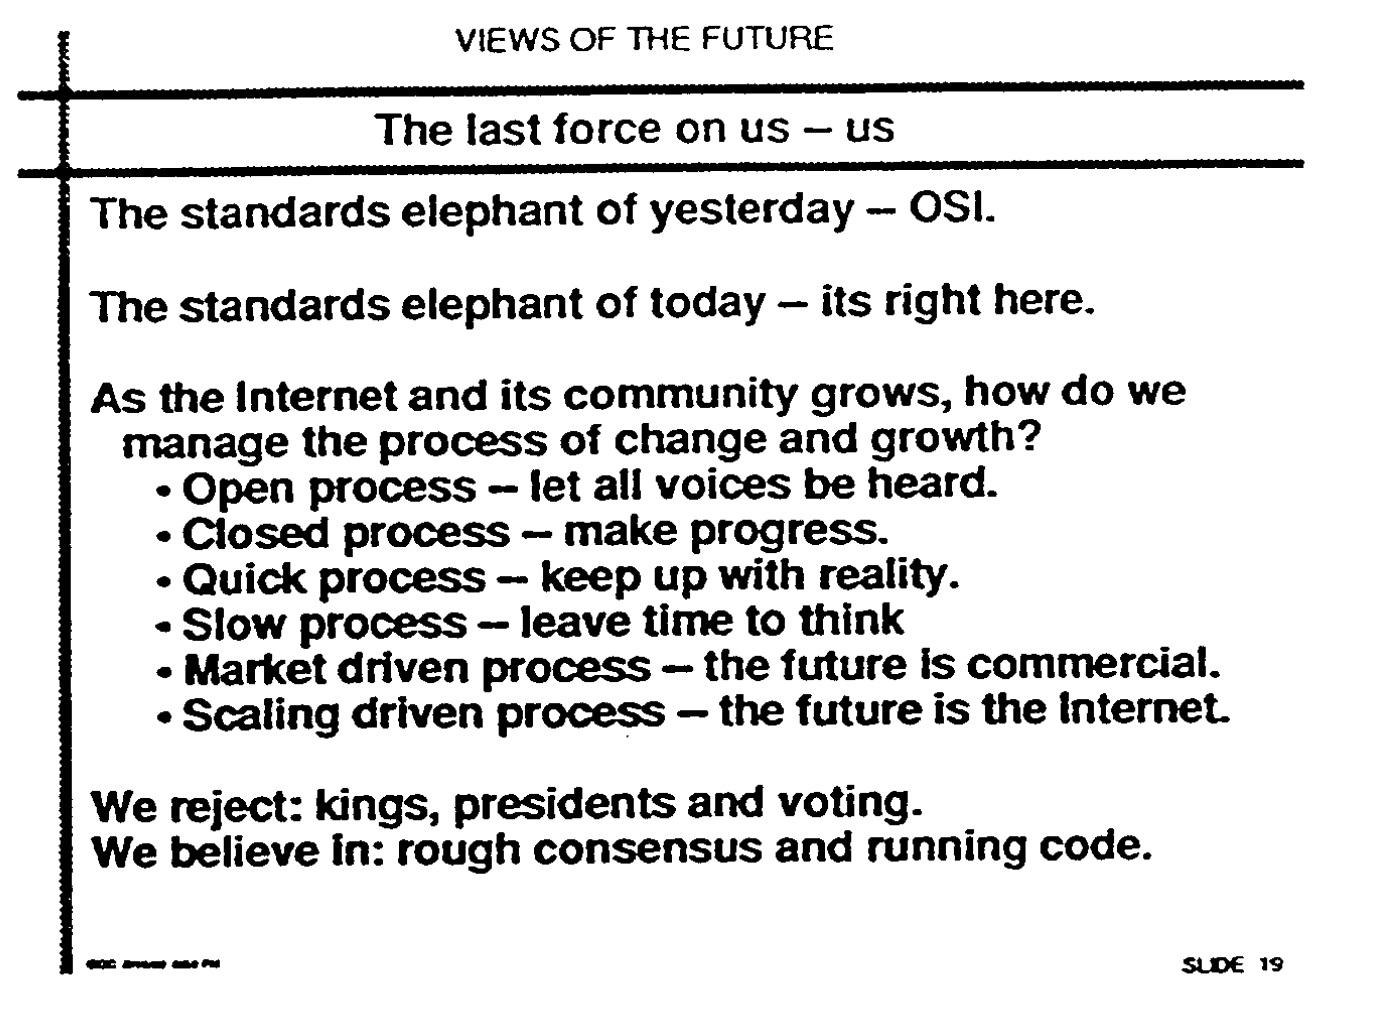
\includegraphics[width=\linewidth]{./images/clark-slide.png}
\label{fig:davidclark}
\caption{A
slide from David Clark's 1992 ``Views of the Future''\citep{clarkCloudyCrystalBall1992}  that contrasts differing visions for the
development process of the future of the internet. The struggle between
engineered order and wild untamedness is summarized forcefully as ``We
reject: kings, presidents and voting. We believe in: rough consensus and
running code''}
\end{figure}

Practically, the differences between these thought communities impact
the tools they build. Aaron Swartz put the approach of the ``neat''
semantic web architects the way he did:

\begin{leftbar}
Instead of the ``let's just build something that works'' attitude that
made the Web (and the Internet) such a roaring success, they brought the
formalizing mindset of mathematicians and the institutional structures
of academics and defense contractors. They formed committees to form
working groups to write drafts of ontologies that carefully listed (in
100-page Word documents) all possible things in the universe and the
various properties they could have, and they spent hours in Talmudic
debates over whether a washing machine was a kitchen appliance or a
household cleaning device.

With them has come academic research and government grants and corporate
R\&D and the whole apparatus of people and institutions that scream
``pipedream.'' And instead of spending time building things, they've
convinced people interested in these ideas that the first thing we need
to do is write standards. (To engineers, this is absurd from the
start---standards are things you write after you've got something
working, not before!) \citep{swartzAaronSwartzProgrammable2013} 
\end{leftbar}

The outcomes of this cultural rift are subtle, but the broad strokes are
clear: the ``scruffies'' largely diverged into the linked data
community, which has taken some of the core semantic web technology like
RDF, OWL, and the like, and developed a broad range of downstream
technologies that have found purchase across information sciences,
library sciences, and other applied domains\sidenote{This isn't a story
  of ``good people'' and ``bad people,'' as a lot of the linked data
  technology also serves as the backbone for abusive technology
  monopolies like google's acquisition of Freebase \citep{iainFreebaseDeadLong2019}  and the profusion of knowledge
  graph-based medical platforms.}. The linked data developers, starting
by acknowledging that no one system can possibly capture everything,
build tools that allow expression of local systems of meaning with the
expectation and affordances for linking data between these systems as an
ongoing social process.

The vision of a totalizing and logically consistent semantic web,
however, has largely faded into obscurity. One developer involved with
semantic web technologies (who requested not be named), captured the
present situation in their description of a still-active developer
mailing list:

\begin{leftbar}
I think that some people are completely detached from practical
applications of what they propose. {[}\ldots{]} I could not follow half
of the messages. these guys seem completely removed from our plane of
existence and I have no clue what they are trying to solve.
\end{leftbar}

This division in thought styles generalizes across domains of
infrastructure, though outside of the linked data and similar worlds the
dichotomy is more frequently between ``neatness'' and ``people doing
whatever'' -- with integration and interoperability becoming nearly
synonymous with standardization. Calls for standardization without
careful consideration and incorporation of existing practice have a
familiar cycle: devise a standard that will solve everything, implement
it, wonder why people aren't using it, funding and energy dissipates,
rinse, repeat\sidenote{There is, of course, an XKCD for that to which we
  make obligatory reference: \url{https://xkcd.com/927/}}. The
difficulty of scaling an exacting vision of how data should be
formatted, the tools researchers should use for their experiments, and
so on is that they require dramatic and sometimes total changes to the
way people do science. The alternative is not between standardization
and chaos, but a potential third way is designing infrastructures that
allow the diversity of approaches, tools, and techniques to be expressed
in a common framework or protocol along with the community
infrastructure to allow the continual negotiation of their relationship.

\hypertarget{taped-on-interfaces-open-loop-user-testing}{%
\subsection{Taped-on Interfaces: Open-Loop User
Testing}\label{taped-on-interfaces-open-loop-user-testing}}

The point of most active competition in many domains of commercial
software is the user interface and experience (UI/UX). To compete,
software companies will exhaustively user-test and refine them with
pixel precision to avoid any potential customer feeling even a
thimbleful of frustration. Scientific software development is largely
disconnected from usability testing, as what little support exists is
rarely tied to it. This, combined with the preponderance of
semi-amateurs and above incentives for developing new packages -- and
thus reduplicating the work of interface development -- make it perhaps
unsurprising that most scientific software is hard to use!

I intend the notion of ``interface'' in an expansive way: In addition to
a graphical user interface (GUI) or set of functions and calling
conventions exposed to the end-user, I am referring generally to all
points of contact with users, developers, and other software. Interfaces
are intrinsically social, and include the surrounding documentation and
experience of use --- part of using software is being able to figure out
how to use it! The favored design idiom of scientific software is the
black box: I implemented an algorithm of some kind, here are the two or
three functions needed to use it, but beneath the surface there be
dragons.

Ideally, software would be designed with developer interfaces and
documentation at multiple scales of complexity to enable clean
entrypoints for developers with differing levels of skill and investment
to contribute. When this kind of design and documentation is
underdeveloped, even widely used projects with excellent top-level
interfaces like \href{https://python-poetry.org/}{poetry} struggle to
respond to the pile of issues
\href{https://github.com/python-poetry/poetry/issues}{thousands deep} as
even users who have spent time reading the source have difficulty
understanding what exactly needs to be fixed and maintainers have to
spend their time triaging them and manually re-explaining the software
hundreds of times\sidenote{For one example of many, see
  \href{https://github.com/python-poetry/poetry/issues/3855}{Issue
  \#3855}, where several users try to make sense of the way poetry
  resolves packages from multiple sources --- a conversation that has
  been happening for more than a year at the time of writing across
  \href{https://github.com/python-poetry/poetry/discussions/4137\#discussioncomment-2320644}{multiple
  related issues}.}.

Additionally, it would include interfaces for use and integration with
other software --- or APIs. While the term ``API'' most commonly refers
to \href{https://en.wikipedia.org/wiki/Web_API}{web APIs}, the term
generally refers to the means by which other programs can interact with
a given program. All programs have some limit to their function, the
question is how other programs are expected to handle them. One
particularly successful approach to program interface design is the Unix
philosophy as articulated by Doug McIlroy and colleagues \citep{mcilroyUNIXTimeSharingSystem1978}  --- which was originally designed
to help build research software. Its first ``make each program do one
thing well'' and second ``expect the output of every program to become
the input to another, as yet unknown, program'' principles inspired a
set of simple tools that can be composed together for complex tasks.
When a program is monolithic and isn't designed to provide access to its
component parts, it becomes difficult to reuse in downstream projects,
potentially reskin with a more friendly user interface, and ultimately
more likely to be a dead-end in a system of shared infrastructure.

Without care given to any of these types of interfaces, the barrier to
use is likely to remain high, the community of co-developers is likely
to remain small, and the labor they expend is less likely to be useful
outside that single project. This, in turn, closes the loop with
incentives to develop new packages and makes another vicious cycle
reinforcing fragmentation\sidenote{Incentivized to develop new packages
  -\textgreater{} need to reinvent interfaces -\textgreater{} hard to
  develop and extend -\textgreater{} incentivized to develop new
  packages}.

\hypertarget{platforms-industry-capture-and-the-profit-motive}{%
\subsection{Platforms, Industry Capture, and the Profit
Motive}\label{platforms-industry-capture-and-the-profit-motive}}

Publicly funded science is an always-irresistable golden goose for
private industry. The fragmented interests of scientists and the
historically light touch of funding agencies on encroaching
privatization means that if some company manages to capture and
privatize a corner of scientific practice they are likely to keep it.
Industry capture has been thoroughly criticized in the context of the
journal system (eg. recently, \citep{brembsReplacingAcademicJournals2021}), and that criticism should
extend to the rest of our infrastructure as information companies seek
to build a for-profit platform system that spans the scientific workflow
(eg. \citep{ElsevierSevenBridges2017}). The mode of privatization
of scientific infrastructure follows the broader software market as a
proliferation of software as a service (SaaS), from startups to
international megacorporations, that rent access to some, typically
proprietary software without selling the software itself.

While in isolation SaaS can make individual components of the
infrastructural landscape easier to access --- and even free!!* --- the
business model is fundamentally incompatible with integrated and
accessible infrastructure. The SaaS model derives revenue from
subscription or use costs, often operating as ``freemium'' models that
make some subset of its services available for free. Even in freemium
models, though, the business model requires that some functionality of
the platform is enclosed and proprietary. To keep the particular domain
of enclosure viable as a profit stream, the proprietor needs to actively
defend against competitors as well as any technology that might fill the
need for the proprietary technology\sidenote{eg. see the complaint in
  State of Texas et al.~v. Google that alleges Google rigs ad markets
  designed to lessen its dominance and uses its control over Chrome and
  Android to create a single, always-on tracking ecosystem owned only by
  them \citep{ReGoogleDigital2021} } (See a more thorough
treatment of platform capitalism in science in \citep{mirowskiFutureOpenScience2018})

As isolated services, one can imagine the practice of science devolving
along a similar path as the increasingly-fragmented streaming video
market: to do my work I need to subscribe to a data storage service, a
cloud computing service, a platform to host my experiments, etc. For
larger software platforms, however, vertical integration of multiple
complementary services makes their impact on infrastructure more
insidious. Locking users into more and more services makes for more and
more revenue, which encourages platforms to be as mutually incompatible
as they can get away with \citep{macinnesCompatibilityStandardsMonopoly2005}. To encourage adoption,
platforms that can offer multiple services may offer one of the services
-- say, data storage -- for free, forcing the user to use the adjoining
services -- say, a cloud computing platform.

Since these platforms are often subsidiaries of information industry
monopolists, scientists become complicit in their often profoundly
unethical behavior of by funneling millions of dollars into them.
Longterm, unconditional funding of wildly profitable journals has
allowed conglomerates like Elsevier to become sprawling surveillance
companies \citep{RELXAnnualReport2020, pooleySurveillancePublishing2021}  that are sucking as much data up
as they can to market derivative products like algorithmic ranking of
scientific productivity \citep{brembsAlgorithmicEmploymentDecisions2021}  and making data sharing
agreements with ICE \citep{biddleLexisNexisProvideGiant2021}. Or
our reliance on AWS and the laundry list of human rights abuses by
Amazon \citep{CriticismAmazon2021}. In addition to lock-in,
dependence on a constellation of SaaS allows the opportunity for
platform-holders to take advantage of their limitations and \emph{sell
us additional services to make up for what the other ones purposely
lack} --- for example Elsevier has taken advantage of our dependence on
the journal system and its strategic disorganization to sell a tool for
summarizing trending research areas for tailoring maximally-fundable
grants \citep{elsevierTopicProminenceSciencea}.

Funding models and incentive structures in science are uniformly aligned
towards the platformatization of scientific infrastructure. Aside from
the corporate doublespeak ``technology transfer'' rhetoric that pervades
the neoliberal university, the relative absence of major funding
opportunities for scientific software developers competitive with the
profit potential from ``industry'' often leaves it as the only viable
career path. The preceding structural constraints on local
infrastructural development strongly incentivize labs and researchers to
rely on SaaS that provides a readymade solution to specific problems.
Distressingly, rather than supporting infrastructural development that
would avoid obligate payments to platform-holders, funding agencies seem
all too happy to lean into them (emphases mine):

\begin{leftbar}
NIH will \textbf{leverage what is available in the private sector,}
either through strategic partnerships or procurement, to create a
workable \textbf{Platform as a Service (PaaS)} environment. {[}\ldots{]}
NIH will partner with cloud-service providers for cloud storage,
computational, and related infrastructure services needed to facilitate
the deposit, storage, and access to large, high-value NIH datasets.
{[}\ldots{]}

NIH's cloud-marketplace initiative will be the first step in a phased
operational framework that \textbf{establishes a SaaS paradigm for NIH
and its stakeholders.} (-NIH Strategic Plan for Data Science, 2018 \citep{NIHStrategicPlan2018})
\end{leftbar}

The articulated plan being to pay platform holders to house data while
also paying for the labor to maintain those databases veers into parody,
haplessly building another triple-pay industry \citep{buranyiStaggeringlyProfitableBusiness2017}  into the economic system
of science --- one can hardly wait until they have the opportunity to
rent their own data back with a monthly subscription. This isn't a
metaphor: the STRIDES program, with the official subdomain
\href{https://web.archive.org/web/20210729131920/https://cloud.nih.gov/}{cloud.nih.gov},
has been authorized to pay \$85 million to cloud providers since 2018.
In exchange, NIH hasn't received any sort of new technology, but
\href{https://web.archive.org/web/20211006003547/https://cloud.nih.gov/enrollment/account-type/}{``extramural''}
scientists receive a maximum discount of 25\% on cloud storage and
``data egress'' fees as well as plenty of training on how to give
control of the scientific process to platform giants \citep{reillyNIHSTRIDESInitiative2021} \sidenote{Their success stories tell
  the story of platform non-integration where scientists have to
  handbuild new tools to manage their data across multiple cloud
  environments: ``We have been storing data in both cloud environments
  because we wanted the ecosystem we are creating to work on both
  clouds'' \citep{STRIDESInitiativeSuccess2020} }. Without
exaggeration, we are paying them to let us pay for something that makes
it so we need to pay them more later.

It is unclear to me whether this is the result of the cultural hegemony
of platform capitalism narrowing the space of imaginable
infrastructures, industry capture of the decision-making process, or
both, but the effect is the same in any case.

\hypertarget{protection-of-institutional-and-economic-power}{%
\subsection{Protection of Institutional and Economic
Power}\label{protection-of-institutional-and-economic-power}}

Aside from information industries, infrastructural deficits are
certainly not without beneficiaries within science --- those that have
already accrued power and status.

Structurally, the adoption of SaaS on a wide scale necessarily
sacrifices the goals of an integrated mass infrastructure as the
practice of research is carved into small, marketable chunks within
vertically integrated technology platforms. Worse, it stands to amplify,
rather than reduce, inequities in science, as the labs and institutes
that are able to afford the tolls between each of the weigh stations of
infrastructure are able to operate more efficiently --- one of many
positive feedback loops of inequity.

More generally, incentives across infrastructures are often misaligned
across strata of power and wealth. Those at the top of a power hierarchy
have every incentive to maintain the fragmentation that prevents people
from competing --- hopefully mostly unconsciously via uncritically
participating in the system rather than maliciously reinforcing it.

This poses an organizational problem: the kind of infrastructure that
unwinds platform ownership is not only unprofitable, it's
\textbf{anti-profitable} -- making it impossible to profit from its
domain of use. That makes it difficult to rally the kind of development
and \href{https://www.snsi.info/}{lobbying} resources that profitable
technology can, requiring organization based on ethical principles and a
commitment to sacrifice control in order to serve a practical need.

The problem is not insurmountable, and there are strategic advantages to
decentralized infrastructure and its development within science.
Centralized technologies and companies might have more concerted power,
but we have \emph{numbers} and can make tools that let us combine small
amounts of labor from many people. We often start (and end) our dreams
of infrastructure with the belief that they will necessarily cost a lot
of \emph{money,} but that's propaganda. Of course development isn't
\emph{free,} but the cost of decentralized technologies is far smaller
than the vast sums of money funneled into industry profits, labor hours
spent compensating for the designed inefficiencies of the platform
model, and the development of a fragmented tool ecosystem built around
them.

Science, as one of few domains of non-economic labor, has the
opportunity to be a seed for decentralized technologies that could
broadly improve not only the health of scientific practice, but the
broader information ecosystem. We can develop a plan and mobilize to
make use of our collective expertise to build tools that have no
business model and no means of development in commercial domains --- we
just need to realize what's at stake and agree that the health of
science is more important than the convenience of the cloud\sidenote{Though
  the system of engineered helpless that convinces us that we're
  incapable of managing our own web infrastructure is not actually as
  reliable and seamless as it claims, as the long history of dramatic
  outages at AWS can show us \citep{lawlerAmazonServerOutage2021, hutchinsonAmazonWebServices2012} } or which journal our papers go
into.

\hypertarget{the-ivies-institutes-and-the-rest-of-us}{%
\section{The Ivies, Institutes, and ``The Rest of
Us''}\label{the-ivies-institutes-and-the-rest-of-us}}

Given these constraints, who can build new digital infrastructure?
Constraints, motivations, and strategies all depend on the circumstance
of those doing the development. The undone work of infrastructure is
being nibbled at around the edges\sidenote{aka doing hard development
  work in sometimes adverse conditions.} by several different kinds of
organization already ranging in scale and structure. A short survey to
give us some notion of how we should seek to organize infrastructure
building:

\hypertarget{institutional-core-facilities}{%
\subsection{Institutional Core
Facilities}\label{institutional-core-facilities}}

Centralized ``core'' facilities are maybe the most typical form of
infrastructure development and resource sharing at the level of
departments and institutions. These facilities can range from minimal to
baroque extravagance depending on institutional resources and whatever
complex web of local history brought them about.

A
\href{https://reporter.nih.gov/project-details/9444124\#sub-Projects}{subproject}
within a
\href{https://projectreporter.nih.gov/project_info_details.cfm?aid=9444124}{PNI
Systems Core} grant echoes a lot of the thoughts here, particularly
regarding effort duplication\sidenote{Thanks a lot to the one-and-only brilliant Dr.~Eartha Mae Guthman for suggesting looking
  at the BRAIN initiative grants as a way of getting insight on core
  facilities.}:

\begin{leftbar}
Creating an Optical Instrumentation Core will address the problem that
much of the technical work required to innovate and maintain these
instruments has shifted to students and postdocs, because it has
exceeded the capacity of existing staff. This division of labor is a
problem for four reasons: (1) lab personnel often do not have sufficient
time or expertise to produce the best possible results, (2) the
diffusion of responsibility leads people to duplicate one another's
efforts, (3) researchers spend their time on technical work at the
expense of doing science, and (4) expertise can be lost as students and
postdocs move on. For all these reasons, we propose to standardize this
function across projects to improve quality control and efficiency.
Centralizing the design, construction, maintenance, and support of these
instruments will increase the efficiency and rigor of our microscopy
experiments, while freeing lab personnel to focus on designing
experiments and collecting data.
\end{leftbar}

While core facilities are an excellent way of expanding access, reducing
redundancy, and standardizing tools \emph{within} an institution, as
commonly structured they can displace work spent on efforts that would
be portable \emph{outside} of the institution. Elite institutions can
attract the researchers with the technical knowledge to develop the
instrumentation of the core and infrastructure for maintaining it, but
this development is only occasionally made usable by the broader public.
The Princeton data science core is an excellent example of a core
facility that does makes its software infrastructure development
\href{https://github.com/BrainCOGS}{public}\sidenote{Project Summary: Core 2, Data Science {[}\ldots{]} In addition, the
  Core will build a data science platform that stores behavior, neural
  activity, and neural connectivity in a relational database that is
  queried by the DataJoint language. {[}\ldots{]} This data-science
  platform will facilitate collaborative analysis of datasets by
  multiple researchers within the project, and make the analyses
  reproducible and extensible by other researchers. {[}\ldots{]}
  \href{https://projectreporter.nih.gov/project\_info\_description.cfm?aid=9444126\&icde=0}{NIH RePORTER}}, which they should be applauded for, but also
illustrative of the problems with a core-focused infrastructure project.
For an external user, the documentation and tutorials are incomplete --
it's not clear to me how one would set this up for my institute, lab, or
data, and there are several places of hard-coded Princeton-specific
values that I am unsure how exactly to adapt\sidenote{Though again, this
  project is exemplary, built by friends, and would be an excellent
  place to start extending towards global infrastructure.}. I would
consider this example a high-water mark, and the median openness of core
infrastructure falls far below it. I was unable to find an example of a
core facility that maintained publicly-accessible documentation on the
construction and operation of its experimental infrastructure or the
management of its facility.

This might be unsurprising given the economic structure of most core
facilities: an institution pays for a core to benefit the institution,
and downstream public benefits are a nice plus but not high up in the
list of concerns (if present at all). Core facilities are thus unlikely
to serve as the source of mass infrastructure, but they do serve as a
point of local coordination within institutions, and so given some
larger means of coordination may still be useful.

\hypertarget{centralized-institutes}{%
\subsection{Centralized Institutes}\label{centralized-institutes}}

Outside of universities, the Allen Brain Institute is perhaps the most
impactful reflection of centralization in neuroscience. The Allen
Institute has, in an impressively short period of time, created several
transformative tools and datasets, including its well-known atlases \citep{leinGenomewideAtlasGene2007}  and the first iteration of its
\href{http://observatory.brain-map.org/}{Observatory} project which
makes a massive, high-quality calcium imaging dataset of visual cortical
activity available for public use. They also develop and maintain
software tools like their
\href{https://allensdk.readthedocs.io/en/latest/}{SDK} and Brain
Modeling Toolkit \href{https://alleninstitute.github.io/bmtk/}{(BMTK)},
as well as a collection of
\href{https://portal.brain-map.org/explore/toolkit/hardware}{hardware
schematics} used in their experiments. The contribution of the Allen
Institute to basic neuroscientific infrastructure is so great that,
anecdotally, when talking about scientific infrastructure it's not
uncommon for me to hear something along the lines of ``I thought the
Allen was doing that.''

Though the Allen Institute is an excellent model for scale at the level
of a single organization, its centralized, hierarchical structure cannot
(and does not attempt to) serve as the backbone for all neuroscientific
infrastructure. Performing single (or a small number of, as in its
also-admirable
\href{https://alleninstitute.org/what-we-do/brain-science/news-press/articles/three-collaborative-studies-launch-openscope-shared-observatory-neuroscience}{OpenScope
Project}) carefully controlled experiments a huge number of times is an
important means of studying constrained problems, but is complementary
with the diversity of research questions, model organisms, and methods
present in the broader neuroscientific community.

Christof Koch, its director, describes the challenge of centrally
organizing a large number of researchers:

\begin{leftbar}
Our biggest institutional challenge is organizational: assembling,
managing, enabling and motivating large teams of diverse scientists,
engineers and technicians to operate in a highly synergistic manner in
pursuit of a few basic science goals \citep{grillnerWorldwideInitiativesAdvance2016} 

These challenges grow as the size of the team grows. Our anecdotal
evidence suggests that above a hundred members, group cohesion appears
to become weaker with the appearance of semi-autonomous cliques and
sub-groups. This may relate to the postulated limit on the number of
meaningful social interactions humans can sustain given the size of
their brain \citep{kochBigScienceTeam2016} 
\end{leftbar}

These institutes too are certainly helpful in building core technologies
for the field, but they aren't necessarily organized for developing
mass-scale infrastructure. They reflect the capabilities and needs of
the institute itself, which are likely to be radically different than a
small lab. They can build technologies on a background of expensive
cloud storage and computation and rely on a team of engineers to
implement and maintain them. So while the tools they make are certainly
\emph{useful} we shouldn't count on them to build the systems we need
for scientists at large.

\hypertarget{meso-scale-collaborations}{%
\subsection{Meso-scale collaborations}\label{meso-scale-collaborations}}

Given the diminishing returns to scale for centralized organizations,
many have called for smaller, ``meso-scale'' collaborations and
consortia that combine the efforts of multiple labs \citep{mainenBetterWayCrack2016}. The most successful consortium of this
kind has been the International Brain Laboratory \citep{abbottInternationalLaboratorySystems2017, woolKnowledgeNetworksHow2020}, a group of 22 labs spread across six countries. They have been
able to realize the promise of big team neuroscience, setting a new
standard for performing reproducible experiments across many labs \citep{laboratoryStandardizedReproducibleMeasurement2020}  and
developing data management infrastructure to match \citep{laboratoryDataArchitectureLargescale2020} \sidenote{Seriously, don't
  miss their extremely impressive
  \href{https://data.internationalbrainlab.org/}{data portal}.}. Their
project thus serves as the benchmark for large-scale collaboration and a
model from which all similar efforts should learn from.

Critical to the IBL's success was its adoption of a flat,
non-hierarchical organizational structure, as described by Lauren E.
Wool:

\begin{leftbar}
IBL's virtual environment has grown to accommodate a diversity of
scientific activity, and is supported by a flexible, `flattened'
hierarchy that emphasizes horizontal relationships over vertical
management. {[}\ldots{]} Small teams of IBL members collaborate on
projects in Working Groups (WGs), which are defined around particular
specializations and milestones and coordinated jointly by a chair and
associate chair (typically a PI and researcher, respectively). All WG
chairs sit on the Executive Board to propagate decisions across WGs,
facilitate operational and financial support, and prepare proposals for
voting by the General Assembly, which represents all PIs. \citep{woolKnowledgeNetworksHow2020} 
\end{leftbar}

They should also be credited with their adoption of a form of consensus
decision-making, \href{https://sociocracy.info}{sociocracy}, rather than
a majority-vote or top-down decisionmaking structure. Consensus
decision-making systems are derived from those developed by
\href{https://rhizomenetwork.wordpress.com/2011/06/18/a-brief-history-of-consenus-decision-making/}{Quakers
and some Native American nations}, and emphasize collective consent
rather than the will of the majority.

The infrastructure developed by the IBL is impressive, but its focus on
a single experiment makes it difficult to expand and translate to
widescale use. The hardware for the IBL experimental apparatus is
exceptionally well-documented, with a
\href{https://figshare.com/articles/preprint/A_standardized_and_reproducible_method_to_measure_decision-making_in_mice_Appendix_3_IBL_protocol_for_setting_up_the_behavioral_training_rig/11634732}{complete
and detailed build guide} and
\href{https://figshare.com/articles/online_resource/A_standardized_and_reproducible_method_to_measure_decision-making_in_mice_CAD_files_for_behavior_rig/11639973}{library
of CAD parts}, but the documentation is not modularized such that it
might facilitate use in other projects, remixed, or repurposed. The
\href{https://github.com/int-brain-lab/iblrig}{experimental software} is
similarly single-purpose, a chimeric combination of Bonsai \citep{lopesBonsaiEventbasedFramework2015}  and
\href{https://github.com/pybpod/pybpod}{PyBpod}
\href{https://github.com/int-brain-lab/iblrig/tree/master/tasks/_iblrig_tasks_ephysChoiceWorld}{scripts}.
It unfortunately
\href{https://iblrig.readthedocs.io/en/latest/index.html}{lacks} the
API-level documentation that would facilitate use and modification by
other developers, so it is unclear to me, for example, how I would use
the experimental apparatus in a different task with perhaps slightly
different hardware, or how I would then contribute that back to the
library. The experimental software, according to the
\href{https://figshare.com/articles/preprint/A_standardized_and_reproducible_method_to_measure_decision-making_in_mice_Appendix_3_IBL_protocol_for_setting_up_the_behavioral_training_rig/11634732}{PDF
documentation}, will also not work without a connection to an
\href{https://github.com/cortex-lab/alyx}{alyx} database. While alyx was
intended for use outside the IBL, it still has
\href{https://github.com/cortex-lab/alyx/blob/07f481f6bbde668b81ad2634f4c42df4d6a74e44/alyx/data/management/commands/files.py\#L188}{IBL-specific}
and
\href{https://github.com/cortex-lab/alyx/blob/07f481f6bbde668b81ad2634f4c42df4d6a74e44/alyx/data/fixtures/data.datasettype.json\#L29}{task-specific}
values in its source-code, and makes community development difficult
with a similar \href{https://alyx.readthedocs.io/en/latest/}{lack} of
API-level documentation and requirement that users edit the library
itself, rather than temporary user files, in order to use it outside the
IBL.

My intention is not to denigrate the excellent tools built by the IBL,
nor their inspiring realization of meso-scale collaboration, but to
illustrate a problem that I see as an extension of that discussed in the
context of core facilities --- designing infrastructure for one task, or
one group in particular makes it much less likely to be portable to
other tasks and groups. This argument is much more contingent on the
specific circumstances of the consortium than the prior arguments about
core facilities and institutes: when organized with mass-infrastructure
in mind, collaborations between semi-autonomous groups across
institutions could be a powerful mode of tool development.

It is also unclear how replicable these consortia are, and whether they
challenge, rather than reinforce technical inequity in science.
Participating in consortia systems like the IBL requires that labs have
additional funding for labor hours spent on work for the consortium, and
in the case of graduate students and postdocs, that time can conflict
with work on their degrees or personal research which are still far more
potent instruments of ``remaining employed in science'' than
collaboration. In the case that only the most well-funded labs and
institutions realize the benefits of big team science without explicit
consideration given to scientific equity, mesoscale collaborations could
have the unintended consequence of magnifying the skewed distribution of
access to technical expertise and instrumentation.

The central lesson of the IBL, in my opinion, is that governance
matters. Even if a consortium of labs were to form explicitly to build
mass-scale digital infrastructure, without a formal system to ensure
contributors felt heard and empowered to shape the project it would soon
become unfocused or unsustainable. Even if this system is not perfect,
with some labor still falling unequally on some researchers, it is a
promising model for future collaborative consortia.

\hypertarget{the-rest-of-us}{%
\subsection{The rest of us\ldots{}}\label{the-rest-of-us}}

Outside of ivies with rich core facilities, institutes like the Allen,
or nascent multi-lab consortia, the rest of us are largely on our own,
piecing together what we can from proprietary and open source
technology. The world of open source scientific software has plenty of
energy and lots of excellent work is always being done, though
constrained by the circumstances of its development described briefly
above. Anything else comes down to whatever we can afford with remaining
grant money, scrape together from local knowledge, methods sections,
begging, borrowing, and (hopefully not too much) stealing from
neighboring labs.

The state of broader scientific deinfrastructuring is perhaps to be
expected given our relationship to informational monopolies that in some
part depend on it, but unlike many other industries or professions there
is reason for hope in science. Science is packed with people with an
enormous diversity of skills, resources, and perspectives. Publicly
funded science is relatively unique as a labor system that does not
strictly depend on profit. There is widespread discontent with the
systems of scientific practice, and so the question becomes how we can
organize our skill, labor, and energy to rebuild the systems that
constrain us.

A third option from the standardization offered by centralization and
the blooming, buzzing, beautiful chaos of disconnected open-source
development is that of decentralized systems, and with them we might
build the means by which the ``rest of us'' can mutually benefit by
organizing our knowledge and labor.

We don't need to wait for permission from a memo from a funding body or
the founding of some new organization. We do have to recognize that
while we might have very different roles to play, we are all responsible
for the state of digital scientific infrastructure. We should take
courage and purpose in knowing that we are not alone, and that our
problems are just one reflection of the model of digital enclosure and
surveillance that defines the information economy. There is no need for
distance or animosity with the other modes of organization described
above, as if what we intend to build is truly useful to \emph{everyone}
except those that profit from its absence, then that certainly includes
them. Shunting the vision of a better future onto some as-yet formed
effort is precisely the trap we should avoid: our existing organizations
\emph{should} be a part of the work of rebuilding our infrastructure
precisely because we should be reconsidering the ways that \emph{we,
ourselves} work. Seeing a subscription to this platform monopolist's
cloud, or that knowledge baron's prestige hierarchy as not being a
value-neutral decision begs an alternative from people, labs, and
institutions alike. The diversity in what that means for different
groups is a \emph{strength,} not a weakness, but it does require some
shared vision and notion of how to get there. The rest of the paper is
an attempt to draft one.

\hypertarget{a-draft-of-decentralized-scientific-infrastructure}{%
\chapter{A Draft of Decentralized Scientific
Infrastructure}\label{a-draft-of-decentralized-scientific-infrastructure}}

What should we build?

The infrastructural systems I will describe here are similar to previous
notions of ``grass-roots'' science articulated within systems
neuroscience \citep{mainenBetterWayCrack2016}, ``small tech''
\citep{balkanSmallTechnologyFoundation}  or the anti software
software club's manifesto \citep{kaplanPartAntisoftwareAction2020}  in the web development world , and shares some of the motivations
of the \href{https://solidproject.org/}{Solid project} \citep{sambraSolidPlatformDecentralized2016}, but ultimately draws from a
set of ideas with broad and deep history in many domains of computing.
My intention is to provide a more prescriptive scaffolding for their
design and implementation as a way of painting a picture of what science
could be like. This sketch is not intended to be final, but a starting
point for further negotiation and refinement.

Throughout this section, when I am referring to any particular piece of
software I want to be clear that I don't intend to be dogmatically
advocating that software \emph{in particular}, but software \emph{like
it} that \emph{shares its qualities} --- no snake oil is sold in this
document. Similarly, when I describe limitations of existing tools,
without exception I am describing a tool or platform I love, have
learned from, and think is valuable --- learning from something can mean
drawing respectful contrast! Many of these technologies have long and
torrid social histories, and so when invoked as examples I don't
necessarily mean to import along with them all the unmentioned baggage
that might accompany them\sidenote{As one example, while I will write
  about \href{https://www.w3.org/DesignIssues/LinkedData.html}{linked
  data}, I don't necessarily mean it in precisely the original
  instantiation as an irrevocable URI/RDF/SPARQL-only web, but do draw
  on its triplet link structure.}.

\hypertarget{design-principles}{%
\section{Design Principles}\label{design-principles}}

I won't attempt to derive a definition of decentralized systems from
first principles here, but from the constraints described above, some
design principles that illustrate the idea emerge naturally. For the
sake of concreteness, in some of these I will draw from the
architectural principles of the internet protocols (specifically
TCP/IP): the most successful decentralized digital technology project to
date.

\hypertarget{protocols-not-platforms}{%
\subsection{Protocols, not Platforms}\label{protocols-not-platforms}}

Much of the basic technology of the internet was developed as protocols
that describe the basic attributes and operations of a process. A simple
and common example is email over SMTP (Simple Mail Transfer Protocol)
\citep{Rfc5321SimpleMail}. SMTP describes a series of steps that
email servers must follow to send a message: the sender initiates a
connection to the recipient server, the recipient server acknowledges
the connection, a few more handshake steps ensue to describe the senders
and receivers of the message, and then the data of the message is
transferred. Any software that implements the protocol can send emails
to and from any other. The protocol basis of email is the reason why it
is possible to send an email from a gmail account to a hotmail account
(or any other hacky homebrew SMTP client) despite being wholly different
pieces of software.

In contrast, \emph{platforms} provide some service with a specific body
of code usually without any pretense of generality. In contrast to email
over SMTP, we have grown accustomed to not being able to send a message
to someone using Telegram from WhatsApp, switching between multiple
mutually incompatible apps that serve nearly identical purposes.
Platforms, despite being \emph{theoretically} more limited than
associated protocols, are attractive for many reasons: they provide
funding and administrative agencies a single point of contracting and
liability, they typically provide a much more polished user interface,
and so on. These benefits are short-lived, however, as the inevitable
toll of lock-in and shadowy business models is realized.

By virtue of being intended for use by many independent organizations
rather than under the sole control of a platform-holder, protocols are a
complicated political effort that embed and facilitate systems of belief
and power (see re: TCP/IP \citep{larsenPoliticalNatureTCP2012},
ActivityPub \citep{lemmer-webberStandardsDivisionsCollaboration2018}). For example, in order to arrive at a version of TCP/IP that kept
the intermediate relays relatively simple at the expense of reliability,
the manufacturer of the ``smart'' relays had to be excluded from the
group. TCP/IP's success was not inevitable: it was one of several
protocols, becoming the default over proprietary competitors from
telecommunication and network hardware companies because of some
combination of timing, its relative absence of bureaucracy, and
institutional adoption (depending on who does the accounting)\citep{larsenPoliticalNatureTCP2012}.

Seemingly prosocial protocols can be used by industries to preempt an
alternative that would undermine their profit model --- a notable
example for academics being the DOI system, created in order for
publishers to preserve control over their intellectual property \citep{rosenblattDigitalObjectIdentifier1997}. The STM
association\sidenote[][-6cm]{The global trade association of publishers that
  serves as its lobbying and propaganda arm.} hastily\sidenote[][-5cm]{The
  description provided by the ``official'' CrossRef 10 year
  retrospective paints a picture of panicked executives making an
  announcement for something they didn't have a clear picture of yet,
  but it would be \emph{something} to compete with pubmed:

  ``We decided to issue an announcement of a broad STM reference linking
  initiative. It was, of course, a strategic move only, since we had
  neither plan nor prototype.

  A small group led by Arnoud de Kemp of Springer-Verlag met in an
  adjacent room immediately following the Board meeting to draft the
  announcement, which was distributed to all attendees of the STM annual
  meeting the following day and published in an STM membership
  publication.

  Campbell recalled running into Bolman and Swanson (neither of whom was
  then on the STM Board) in the hotel lobby immediately after the
  drafting of the announcement. Their astonishment at hearing what had
  just transpired was matched by Campbell's own on learning what they
  had been working on. {[}\ldots{]}

  Bolman and Swanson chose to seize the moment, and called an ad hoc
  meeting the following evening, Tuesday, October 12, to announce their
  venture and assemble a coalition of publishers to launch it.
  {[}\ldots{]}

  The potential benefit of the service that would become CrossRef was
  immediately apparent. Organizations such as AIP and IOP (Institute of
  Physics) had begun to link to each other's publications, and the
  impossibility of replicating such one-off arrangements across the
  industry was obvious. As Tim Ingoldsby later put it, ``All those
  linking agreements were going to kill us.'' \citep{crossrefFormationCrossRefShort2009}} threw its weight behind the DOI-X initiative at its 1999
meeting. The impending creation of PubMed Central by the National
Library of Medicine (and see then-NIH Director Harold Varmus' and others
self-described ``radical'' departure from publishers with what became
PLoS \citep{varmusArtPoliticsScience2009, robertsBuildingGenBankPublished2001}) posed an existential threat to
for-profit publishing. At the time there was no unified means of linking
to scholarly work\sidenote{It is hard to appreciate in retrospect how
  radical URLs/URIs were at the time --- it might seem trivial to us now
  to be able to arbitrarily link to different locations on the internet,
  but before the internet linking was a carefully controlled process
  within publishing, looking more like ISBN and ISSNs than hyperlinks.},
and bilateral publisher-publisher linking deals threatened the smooth
operation of business, so an NIH-owned platform might have made journals
might lose their status as the obligate dissemination platform.
According to Bob Campbell, STM chair at the time: ``our consensus was
that publishers should be the ones doing the linking.'' Unlike the
anarchic URI/URL, The DOI system requires a registrar (denoted by the
prefix before the slash, \texttt{doi:10.xxxx/yyyyy}) to create DOI names
\citep{isoISO2632420122012}. In the US, that means being an
institution with an approved
\href{https://www.crossref.org/services/content-registration/}{CrossRef
membership}, which
\href{https://www.crossref.org/membership/terms/}{requires} members not
to link to intellectual property infringing content, and to use DOIs as
their default reference links to other works. Effectively, though it is
an ``open\sidenote{Reading the standard costs 88 Swiss Francs.}''
standard, the DOI system ensures that publishers remain in control of
what counts as scholarly work \citep{crossrefFormationCrossRefShort2009}.

When approaching protocols, we should do so with humility and caution:
work in smaller teams with shared visions with the intention of rough
consensus around multiple instances of working code. We should refuse
participation by the wide range of industries and interest groups
circling each domain of infrastructure, their protocols and standards
are siren songs.

\hypertarget{integration-not-invention}{%
\subsection{Integration, not
Invention}\label{integration-not-invention}}

At the advent of the internet protocols, several different institutions
and universities had already developed existing network infrastructures,
and so the ``top level goal'' of IP was to ``develop an effective
technique for multiplex utilization of existing interconnected
networks,'' and ``come to grips with the problem of integrating a number
of separately administered entities into a common utility'' \citep{clarkDesignPhilosophyDARPA1988}. As a result, IP was developed as a
`common language' that could be implemented on any hardware, and upon
which other, more complex tools could be built. This is also a cultural
practice: when the system doesn't meet some need, one should try to
extend it rather than building a new, separate system --- and if a new
system is needed, it should be interoperable with those that exist.

This point is practical as well as tactical: to compete, an emerging
protocol should integrate or be capable of bridging with the
technologies that currently fill its role. A new database protocol
should be capable of reading and writing existing databases, a new
format should be able to ingest and export to existing formats, and so
on. The degree to which switching is seamless is the degree to which
people will be willing to switch.

This principle runs directly contrary to the current incentives for
novelty and fragmentation and the dominant economic model of software
platforms, which must be counterbalanced by design choices elsewhere.

\hypertarget{embrace-heterogeneity-be-uncoercive}{%
\subsection{Embrace Heterogeneity, Be
Uncoercive}\label{embrace-heterogeneity-be-uncoercive}}

In addition to integrating with existing systems, it must be
straightforward for unanticipated future development to be integrated to
accommodate unanticipated needs and practices. This idea is related to
``the test of independent invention'', summarized with the question ``if
someone else had already invented your system, would theirs work with
yours?'' \citep{berners-leePrinciplesDesign1998}. Rather than
attempting to \emph{a priori} divine a single perfect universal
protocol, we should design multiple with extensibility in mind (see this
discussion of the extensibility models of ActivityPub to XMPP \citep{schubertActivityPubFinalThoughts2019}  and Christopher Yoo's
description of the tradeoffs of the internet's layered protocols \citep{yooProtocolLayeringInternet2013}) to leave open the opportunity
for porting functionality between them.

This principle also has tactical elements. An uncoercive system allows
users to gradually adopt it rather than needing to adopt all of its
components in order for any one of them to be useful. We shouldn't rely
on potential users making dramatic changes to their existing practices.
For example, an experimental framework should not insist on a prescribed
set of supported hardware and rigid formulation for describing
experiments. Instead it should provide affordances that give a clear way
for users to extend the system to fit their needs \citep{carpenterRFC1958Architectural1996}.There always needs to be a
\emph{benefit} to adopting further components of the system to encourage
\emph{voluntary} adoption, but it should never be \emph{compulsory.} For
example, again from experimental frameworks, it should be possible to
use it to control experimental hardware without needing to use the rest
of the experimental design, data storage, and interface system. To some
degree this is accomplished with a modular system design where designers
are mindful of keeping the individual modules independently useful.

A noncoercive architecture also prioritizes the ease of leaving. Though
this is somewhat tautological to protocol-driven design, specific care
must be taken to enable export and migration to new systems.
Multiplicity of design and making leaving easy help ensure that early
missteps in development of the system are not fatal, preventing lock-in
to a component that becomes fixed and stagnant.

\hypertarget{empower-people-not-systems}{%
\subsection{Empower People, not
Systems}\label{empower-people-not-systems}}

Because IP was initially developed as a military technology by DARPA, a
primary design constraint was survivability in the face of failure. The
model adopted by internet architects was to move as much functionality
as possible from the network itself to the end-users of the network ---
rather than the network itself guaranteeing a packet is transmitted, the
sending computer will do so by requiring a response from the recipient
\citep{clarkDesignPhilosophyDARPA1988}.

For infrastructure, we should make tools that don't require a central
team of developers to maintain, a central server-farm to host data, or a
small group of people to govern. Whenever possible, data, software, and
hardware should be self-describing\sidenote{AKA you shouldn't need to
  resort to some external source to understand it. Data should come
  packaged with clear metadata, software should have its own docs, etc.},
so one needs minimal additional tools or resources to understand and use
it. It should never be the case that funding drying up for one node in
the system causes the entire system to fail.

Practically, this means that the tools of digital infrastructure should
be deployable by individual people and be capable of recapitulating the
function of the system without reference to any central authority.
Researchers need to be given control over the function of
infrastructure: from controlling sharing permissions for eg. clinically
sensitive data to assurance that their tools aren't spying on them.
Formats and standards must be negotiable by the users of a system rather
than regulated by a central governance body.

\hypertarget{infrastructure-is-social}{%
\subsection{Infrastructure is Social}\label{infrastructure-is-social}}

The alternative to centralized governing and development bodies is to
build the tools for community control over infrastructural components.
This is perhaps the largest missing piece in current scientific tooling.
On one side, decentralized governance is the means by which an
infrastructure can be maintained to serve the ever-evolving needs of its
users. On the other, a sense of community ownership is what drives
people to not only adopt but contribute to the development of an
infrastructure. In addition to being a source of all the warm fuzzies of
socially affiliative ``community-ness,'' any collaborative system needs
a way of ensuring that the practice of maintaining, building, and using
it is designed to \emph{visibly and tangibly benefit} those that do,
rather than be relegated to a cabal of invisible developers and
maintainers \citep{grudinGroupwareSocialDynamics1994, randallDistributedOntologyBuilding2011}.

Governance and communication tools also make it possible to realize the
infinite variation in application that infrastructures need while
keeping them coherent: tools must be built with means of bringing the
endless local conversations and modifications of use into a common space
where they can become a cumulative sense of shared memory.

I will return to this idea in
\protect\hyperlink{archives-need-communities}{Archives Need Communities}
in the context of social dynamics of private bittorrent trackers, as
well as propose a set of basic communication and governance tools in
\protect\hyperlink{rebuilding-scientific-communication}{Rebuilding
Scientific Communication}.

\hypertarget{usability-matters}{%
\subsection{Usability Matters}\label{usability-matters}}

It is not enough to build a technically correct technology and assume it
will be adopted or even useful, it must be developed embedded within
communities of practice and \emph{be useful for solving problems that
people actually have.} We should learn from the struggles of the
semantic web project. Rather than building a fully prescriptive and
complete system first and deploying it later, we should develop tools
whose usability is continuously improved \emph{en route} to a (flexible)
completed vision.

The adage from RFC 1958\sidenote{A ``request for comment'' from the
  Network Working Group of the Internet Engineering Task Force on the
  architecture of the internet. The IETF designs many of the protocols
  that serve as the backbone of the internet.} ``nothing gets
standardized until there are multiple instances of running code'' \citep{carpenterRFC1958Architectural1996}  captures the dual nature of
the constraint well. Workable standards don't emerge until they have
been extensively tested in the field, but development without an eye to
an eventual protocol won't make one.

We should read the
\href{https://en.wikipedia.org/wiki/Embrace,_extend,_and_extinguish}{gobbling
up} of open protocols into proprietary platforms that defined ``Web
2.0'' as instructive\sidenote{(in addition to a demonstration of the raw
  power of concentrated capital, of course)}\citep{markoffTomorrowWorldWide1996}. \emph{Why} did Slack outcompete
IRC?\sidenote{\href{https://en.wikipedia.org/wiki/Internet_Relay_Chat}{IRC},
  internet relay chat, was a messaging system that served many of the
  same functions as the group messaging program
  \href{https://slack.com/}{Slack} serves now. Also see its more active
  cousin \href{https://en.wikipedia.org/wiki/XMPP}{XMPP}} The answer is
relatively simple: it was relatively simple to use. Using a contemporary
example, to
\href{https://matrix-org.github.io/synapse/latest/setup/installation.html}{set
up a Synapse server} to communicate over
\href{https://matrix.org/docs/spec/}{Matrix} one has to wade through
dozens of shell commands, system-specific instructions, potential
conflicts between dependent packages, set up an SQL server\ldots{} and
that's just the backend, we don't even have a frontend client yet! In
contrast, to use Slack you download the app, give it your email, and
you're off and running.

The control exerted by centralized systems over their system design does
give certain structural advantages to their usability, and their
for-profit model gives certain advantages to their development process.
There is no reason, however, that decentralized systems \emph{must} be
intrinsically harder to use, we just need to focus on user experience to
a degree comparable to centralized platforms: if it takes a college
degree to turn the water on, that ain't infrastructure.

People are smart, they just get frustrated easily and have other things
to do on a deadline. We have to raise our standards of design such that
we don't expect users to have even a passing familiarity with
programming, attempting to build tools that are truly general use. We
can't just design a peer-to-peer system, we need to make the data
ingestion and annotation process automatic, effortless, and expressive.
We can't just build a system for credit assignment, it needs to happen
as an automatic byproduct of using the system. We can't just make tools
that \emph{work,} they need to \emph{feel good to use.}

Centralized systems also have intrinsic limitations that provide
openings for decentralized systems, like cost, incompatibility with
other systems, restrictions on independent extension, and opacity of
function. The potential for decentralized systems to capture the
independent development labor of all of its users, rather than just that
of a core development team, is one means of competition. If a system is
sufficiently easy to adopt, at least comparable to prior tooling, and
gives people a satisfying means of having their work accepted and
valued, the social and technical joy might be enough to outweigh the
inertia of change and the convenience of centralized systems.

With these principles in mind, and drawing from other knowledge
communities solving similar problems: internet infrastructure,
library/information science, peer-to-peer networks, and radical
organizing, I conceptualize a system of distributed infrastructure for
(neuro)science as three objectives:
\protect\hyperlink{shared-data}{\textbf{shared data}},
\protect\hyperlink{shared-tools}{\textbf{shared tools}}, and
\protect\hyperlink{shared-knowledge}{\textbf{shared knowledge}}.

\changelocaltocdepth{2}
\hypertarget{shared-data}{%
\section{Shared Data}\label{shared-data}}

\hypertarget{formats-as-onramps}{%
\subsection{Formats as Onramps}\label{formats-as-onramps}}

The shallowest onramp towards a generalized data infrastructure is to
make use of existing discipline-specific standardized data formats. As
will be discussed later, a truly universal pandisciplinary format is
impossible and undesirable, but to arrive at the alternative we should
first congeal the wild west of unstandardized data into a smaller number
of established formats.

Data formats consist of some combination of an abstract specification,
an implementation in a particular storage medium, and an API for
interacting with the format. I won't dwell on the particular qualities
that a particular format needs, assuming that most that would be adopted
would abide by FAIR principles.

There are a dizzying number of scientific data formats \citep{teamScientificDataFormats}, so a comprehensive treatment is
impractical here and I will use Neurodata Without Borders:N (NWB)\citep{rubelNWBAccessibleData2019a}  as an example. NWB is the de facto
standard for systems neuroscience, adopted by many institutes and labs,
though far from universally. NWB
\href{https://www.nwb.org/nwb-software/}{consists of} a
\href{https://schema-language.readthedocs.io/en/stable/}{specification
language}, a \href{https://nwb-schema.readthedocs.io/en/stable/}{schema
written in that language}, a
\href{https://nwb-storage.readthedocs.io/en/stable/}{storage
implementation in hdf5}, and an
\href{https://pynwb.readthedocs.io/en/stable/}{API for interacting with
the data}. They have done an admirable job of engaging with community
needs \citep{rubelNeurodataBordersEcosystem2021}  and making a
modular, extensible format ecosystem.

The major point of improvement for NWB, and I imagine many data
standards, is the ease of conversion and use. The conversion API
requires extensive programming, knowledge of the format, and navigation
of several separate tutorial documents. This means that individual labs,
if they are lucky enough to have some partially standardized format for
the lab, typically need to write (or hire someone to write) their
\href{https://github.com/catalystneuro/tank-lab-to-nwb}{own} software
\href{https://github.com/catalystneuro/mease-lab-to-nwb}{library} for
conversion.

Without being prescriptive about its form, substantial interface
development is needed to make mass conversion possible. It's usually
untrue that unstandardized data had \emph{no structure,} and researchers
are typically able to articulate it -- ``the filenames have the
collection date followed by the subject id,'' and so on. Lowering the
barriers to conversion mean designing tools that match the descriptive
style of folk formats, for example by prompting them to describe where
each of an available set of metadata fields are located in their data.
It is not an impossible goal to imagine a piece of software that can be
downloaded and with minimal recourse to reference documentation allow
someone to convert their lab's data within an afternoon.

NWB also has an extension interface, which allows, for example, data
from common hardware and software tools to be more easily described in
the format. These are registered in an
\href{https://nwb-extensions.github.io/}{extensions catalogue}, but at
the time of writing it is relatively sparse. The preponderance of
lab-specific conversion packages relative to extensions is indicative of
an interface and community tools problem: presumably many people are
facing similar conversion problems, but because there is not a place to
share these techniques in a human-readable way, the effort is duplicated
in dispersed codebases. We will return to some possible solutions for
knowledge preservation and format extension when we discuss tools for
\protect\hyperlink{shared-knowledge}{shared knowledge}.

For the sake of the rest of the argument, let us assume that some
relatively trivial conversion process exists to subdomain-specific data
formats and we reach some reasonable penetrance of standardization. The
interactions with the other pieces of infrastructure that may induce and
incentivize conversion will come later.

\hypertarget{peer-to-peer-as-a-backbone}{%
\subsection{Peer-to-peer as a
Backbone}\label{peer-to-peer-as-a-backbone}}

We should adopt a \emph{peer-to-peer} system for storing and sharing
scientific data. There are, of course
\href{https://www.dandiarchive.org/}{many}
\href{https://openneuro.org/}{existing}
\href{https://www.brainminds.riken.jp/}{databases}
\href{https://biccn.org/}{for} scientific data, ranging from
domain-general like \href{https://figshare.com/}{figshare} and
\href{https://zenodo.org/}{zenodo} to the most laser-focused
subdiscipline-specific. The notion of a database, like a data standard,
is not monolithic. As a simplification, they consist of at least the
hardware used for storage, the software implementation of read, write,
and query operations, a formatting schema, some API for interacting with
it, the rules and regulations that govern its use, and especially in
scientific databases some frontend for visual interaction. For now we
will focus on the storage software and read-write system, returning to
the format, regulations, and interface later.

Centralized servers\sidenote{This applies to centrally managed
  traditional servers as well as rented space on larger CDNs like AWS,
  but in the case of the CDN the constraint is from their pricing model.}
are fundamentally constrained by their storage capacity and bandwidth,
both of which cost money. In order to be free, database maintainers need
to constantly raise money from donations or grants in order to pay for
both. Funding can never be infinite, and so inevitably there must be
some limit on the amount of data that someone can upload and the speed
at which it can serve files\sidenote{As I am writing this, I am getting
  a (very unscientific sample of n=1) maximum speed of 5MB/s on the
  \href{https://osf.io}{Open Science Framework}}. Centralized servers
are also intrinsically out of the control of their users, requiring them
to abide whatever terms of use the server administrators set. Even if
the database is carefully backed up, it serves as a single point of
infrastructural failure, where if the project lapses then at worst data
will be irreversibly lost, and at best a lot of labor needs to be
expended to exfiltrate, reformat, and rehost the data. The same is true
of isolated, local, institutional-level servers and related database
platforms, with the additional problem of skewed funding allocations
making them unaffordable for many researchers.

Peer-to-peer (p2p) systems solve many of these problems, and I argue are
the only type of technology capable of making a database system that can
handle the scale of all scientific data. They are also not new for
science, used in projects like
\href{https://academictorrents.com/}{AcademicTorrents.com} \citep{cohenAcademicTorrentsCommunityMaintained2014, loAcademicTorrentsScalable2016}  or the now defunct BioTorrents \citep{langilleBioTorrentsFileSharing2010}. Whether we acknowledge it
or not, most scientific work is already available on p2p networks via
sci-hub and library genesis \citep{himmelsteinSciHubProvidesAccess2018, sci-hubTorrentHealthTracker2022, bookwarriorLibraryGenesisDecentralized2021}.

There is an enormous degree of variation between p2p systems\sidenote{Peer
  to peer systems are, maybe predictably, a whole academic
  subdiscipline. See \citep{shenHandbookPeertoPeerNetworking2010} 
  for reference.}, but they share a set of architectural advantages. The
essential quality of any p2p system is that rather than each participant
in a network interacting only with a single server that hosts all the
data, everyone hosts data and interacts directly with each other.

For the sake of concreteness, we can consider a (simplified) description
of Bittorrent \citep{cohenBitTorrentProtocolSpecification2017},
arguably the most successful p2p protocol. To share a collection of
files, a user creates a \texttt{.torrent} file with their Bittorrent
client which consists of a
\href{https://en.wikipedia.org/wiki/Cryptographic_hash_function}{cryptographic
hash}, or a string that is unique to the collection of files being
shared; and a list of ``trackers.'' A tracker, appropriately, keeps
track of the \texttt{.torrent} files that have been uploaded to it, and
connects users that have or want the content referred to by the
\texttt{.torrent} file. The uploader (or seeder) then leaves a
\href{https://en.wikipedia.org/wiki/Glossary_of_BitTorrent_terms\#Client}{torrent
client} open waiting for incoming connections. Someone who wants to
download the files (a leecher) will then open the \texttt{.torrent} file
in their client, which will then ask the tracker for the IP addresses of
the other peers who are seeding the file, directly connect to them, and
begin downloading. So far so similar to standard client-server systems,
but say another person wants to download the same files before the first
person has finished downloading it: rather than \emph{only} downloading
from the original seeder, the new leecher downloads from \emph{both} the
original seeder and the first leecher by requesting pieces of the file
from each until they have the whole thing. Leechers are incentivized to
share among each other to prevent the seeders from spending time
reuploading the pieces that they already have, and once they have
finished downloading they become seeders themselves.

From this very simple example, we can articulate a number of attractive
qualities of p2p systems:

\begin{itemize}

\item
  First, p2p systems are extremely \textbf{inexpensive to maintain}
  since they take advantage of the existing bandwidth and storage space
  of the computers in the swarm. Near the height of its popularity in
  2009, The Pirate Bay, a notorious bittorrent tracker \citep{vandersarPirateBayFive2011}, was estimated to cost \$3,000 per
  month to maintain while serving approximately 20 million peers \citep{roettgersPirateBayDistributing2009}. According to a database
  dump from 2013 \citep{PirateBayArchiveteam2020}, multiplying
  the size of each torrent by the number of seeders (ignoring any
  partial downloads from leechers), the approximate instantaneous amount
  of data stored by The Pirate Bay was \textasciitilde26 Petabytes. The
  comparison to centralized services is not straightforward, since it is
  hard to evaluate the distributed costs of additional storage media (as
  well as the costs avoided by being able to take advantage of existing
  storage infrastructure within labs and institutes), but for the sake
  of illustration: hosting 26PB would cost \$546,000/month with standard
  AWS S3 hosting
  (\href{https://aws.amazon.com/s3/pricing/?nc=sn\&loc=4}{\$0.021/GB/month}).
  On AWS, downloads cost extra
  (\href{https://aws.amazon.com/s3/pricing/?nc=sn\&loc=4}{\$0.05/GB}),
  so the much smaller
  \href{https://academictorrents.com}{academictorrents.com} which
  \href{https://github.com/academictorrents/academictorrents-docs/issues/31\#issuecomment-1155917166}{has
  served} nearly 18PB in 1.3m downloads since 2016 would have cost
  \$900,000 in bandwidth costs alone --- as opposed to the
  \href{https://github.com/academictorrents/academictorrents-docs/issues/31\#issuecomment-1152851111}{literally
  zero dollars} it costs to operate.
\item
  The \textbf{speed} of a bittorrent swarm \emph{increases,} rather than
  decreases, the more people are using it since it is capable of using
  all of the available bandwidth in the system.
\item
  The network is extremely \textbf{resilient} since the data is shared
  across many independent peers in the system. If our goal is to make a
  resilient and robust data architecture, we would benefit by paying
  attention to the tools used in the broader archival community,
  especially the archival communities that are frequent targets of
  governments and intellectual property holders \citep{spiesDataIntegrityLibrarians2017}. Despite more than 15 years of
  concerted effort by governments and intellectual property holders, The
  Pirate Bay is still alive and kicking\sidenote{knock on wood} \citep{kim15YearsPirate2019}. This is because even if the entire
  infrastructure of the tracker is destroyed, as it was in 2006, the
  files are distributed across all of its users, the actual database of
  \texttt{.torrent} metadata is quite small, and the tracker software is
  extraordinarily simple to rehost \citep{vandersarOpenBayNow2014}  -- The Pirate Bay was back online in 2 days. When another
  tracker, what.cd (which we will return to
  \protect\hyperlink{archives-need-communities}{soon}) was shut down, a
  series of successors popped up using the open source tools
  \href{https://github.com/WhatCD/Gazelle}{Gazelle} and
  \href{https://github.com/WhatCD/Ocelot}{Ocelot} that what.cd
  developers built. Within two weeks, one successor site had recovered
  and reindexed 200,000 of its torrents resubmitted by former users \citep{vandersarWhatCdDead2016}. Bittorrent is also used by archival
  groups with little funding like
  \href{https://wiki.archiveteam.org/index.php/Main_Page}{Archive Team},
  who struggled -- but eventually succeeded -- to disseminate their
  \href{https://wiki.archiveteam.org/index.php/GeoCities_Project}{geocities
  archive} over a single ``crappy cable modem'' \citep{scottGeocitiesTorrentUpdate2010}.
\item
  The network is extremely \textbf{scalable} since there is no cost to
  connecting new peers and the users of a system expand the storage
  capacity of the system depending on their needs. Rather than having
  one extremely fast data center, the model of p2p systems is to
  leverage many approachable peer/servers.
\end{itemize}

Peer-to-peer systems are not mutually exclusive with centralized
servers: servers are peers too, after all. A properly implemented p2p
system will always be \emph{at least} as fast and have \emph{at least}
as much storage as any alternative centralized server because peers can
use \emph{both} the bandwidth of the server \emph{and} that of any peers
that have the file. In the bittorrent ecosystem large-bandwidth/storage
peers are known as ``seedboxes''\citep{rossiPeekingBitTorrentSeedbox2014}  when they use the bittorrent
protocol, and ``web seeds''\citep{hoffmanHTTPBasedSeedingSpecification}  when they use a protocol built
on top of traditional HTTP. \href{https://archive.org}{Archive.org} has
been distributing all of its materials
\href{https://archive.org/details/bittorrent}{with bittorrent} by using
its servers as web seeds since 2012 and makes this point explicitly:
``BitTorrent is now the fastest way to download items from the Archive,
because the Bittorrent client downloads simultaneously from two
different Archive servers located in two different datacenters, and from
other Archive users who have downloaded these Torrents already.'' \citep{kahle000000Torrents2012} 

p2p systems complement centralized servers in a number of ways beyond
raw download speed, increasing the efficiency and performance of the
network as a whole. Spotify began as a joint client/server and p2p
system \citep{kreitzSpotifyLargeScale2010b}, where when a
listener presses play the central server provides the data until the p2p
system locates peers with a cached copy to download from. The central
server is able to respond quickly and reliably, and is the server of
last resort in the case of rare files that aren't being shared by anyone
else in the network. The p2p system alleviates pressure on the central
server, improving the performance of the network and reducing server
costs.

A peer to peer system is a particularly natural fit for many of the
common circumstances and practices in science, where centralized server
architectures seem (and prove) awkward and inefficient. Most labs,
institutes, or other organized bodies of science have some form of local
or institutional storage systems. In the most frequent cases of sharing
data within a lab or institute, sending it back and forth to some
nationally-centralized server is like walking across the lab by going
the long way around the Earth. That's the method invoked by a Dropbox or
AWS link, which keeps a time-tested p2p system relevant: walking a flash
drive across the lab. The system makes less sense when several people in
the same place need to access the same data at the same time, as is
frequently the case with multi-lab collaborations, or scientific
conferences and workshops. Instead of needing to wait on the 300kb/s
conference wifi bandwidth as it's cheese-gratered across every machine,
we instead could directly beam it between all computers in range
simultaneously, full blast through the decrepit network switch that
won't have seen that much excitement in years.

If we take the suggestion of Andrey Andreev et al.~and invest in server
clusters within institutes \citep{andreevBiologistsNeedModern2021, charlesCommunityDrivenBigOpen2020}, their impact could be multiplied
manyfold by fluidly combining them in a p2p swarm. While the NIH might
be shy to start up another server farm for all scientific data and
prefer to contract with AWS, the rest of us don't have to be. Nervous
university administrators concerned about bandwidth costs should also
favor p2p systems: instead of needing to serve entire datasets to each
person who wants them, the load can be spread out across many institutes
naturally based on the use of the file, and sharing the dataset
internally would cost nothing at all.

So far I have relied on the Extraordinarily Simplified
Bittorrent\sidenote{™️} depiction of a peer to peer system, but there
are many improvements and variants that can address different needs for
scientific data infrastructure.

One obvious need that bittorrent can't currently support is version
control\sidenote{Though the Bittorrent V2 protocol specification \citep{cohenBEP52BitTorrent2017}  adopts a Merkle tree data structure
  which could theoretically support versioned torrents, v2 torrents are
  still not widely supported.}, but more recent p2p systems do.
\href{https://ipfs.io/}{IPFS} functions like ``a single BitTorrent
swarm, exchanging objects within one Git repository.'' \citep{benetIPFSContentAddressed2014} \sidenote{Git, briefly, is a version
  control system that keeps a history of changes of files (blobs) as a
  Merkle DAG: files can be updated, and different versions can be
  branched and reconciled.} Dat \citep{ogdenDatDistributedDataset2017}, specifically designed for data synchronization and versioning,
handles versioning and more. A full description of IPFS is out of scope,
and it has plenty of problems \citep{patsakisHydrasIPFSDecentralised2019}, but for now it suffices to say
p2p systems can handle version control.

Bittorrent swarms are vulnerable to data loss if all the peers seeding a
file disconnect (though the tail is longer than typically assumed, see
\citep{zhangUnravelingBitTorrentEcosystem2011}), but this too can
be addressed with updated p2p system design. A first-order solution to
this problem is a variant of IPFS' notion of `pinning.' Since backup to
lab-level or institutional servers is already commonplace, one peer
could be able to `pin' another and automatically download all the data
that they share. This concept could scale to institutes and national
infrastructure as scientists can request the datasets they'd like to be
saved permanently be pinned.

Another could be something akin to Freenet \citep{clarkeFreenetDistributedAnonymous2001}. Peers could allocate a
certain amount of their unused storage space to be used to automatically
download, cache, and rehost shards of other datasets. Distributing
chunks and encrypting them at rest so the rehoster can't inspect their
contents would make it possible to maintain privacy and network
availability for sensitive data (see, for example,
\href{https://inqlab.net/projects/eris/}{ERIS}). IPFS has an analogous
concept -- BitSwap -- that is makes it into a barter system. Peers who
seek to download will have to `earn' it by finding some chunk of data
that the other peers want, download, and share them, though it seems
like an empirical question whether or not a barter system works or is
necessary.

\href{https://solidproject.org/}{Solid} is a project that almost exactly
meets all these needs \citep{capadisliSolidProtocol2020, sambraSolidPlatformDecentralized2016, SolidP2PFoundation}. Solid
allows people to share data in
\href{https://solidproject.org/about}{Pods}, which let them control
access and distribution across storage system with a unified identity
system. It is implementation-agnostic, and so can support any
peer-to-peer storage and transfer system that complies with its
\href{https://solidproject.org/TR/protocol}{protocol specification}.

There are a number of additional requirements for a peer to peer
scientific data infrastructure, but even these seemingly very technical
problems of versioning and distributed storage show the clear need to
consider the structure of the surrounding social system. What control do
we give to researchers over the version history of their data? Should
people that aren't the originating researcher be able to issue new
versions? What structure of distributed/centralized storage works? How
should we incentivize sharing of excess storage and resources?

Even before considering additional social systems, a p2p structure in
itself implies a different relationship to infrastructure. Scientists
always unavoidably make their data available to at least one person:
themselves; on at least one computer: theirs, and that computer is
usually connected to the internet. With a p2p system that integrates
metadata from domain-specific data formats, that's it, that's all, the
data is already hosted by merely existing. Dust your palms off: open
data achieved. A peer-to-peer backbone for scientific infrastructure
realizes the unnecessarily radical notion that our infrastructure can be
integrated into our daily practices, rather than existing exogenously as
something ``out there.'' It helps us internalize the slyly subversive
notion that \emph{we can build it ourselves} instead of renting
something out of our control from someone else.

Scientists don't need to reinvent the notion of distributed, community
curated data archives from scratch. In addition to scholarly work on the
social systems of digital infrastructure, we can learn from communities
of practice, and there has been no more important and impactful
decentralized archival project than internet piracy.

\hypertarget{archives-need-communities}{%
\subsection{Archives Need Communities}\label{archives-need-communities}}

Why do hundreds of thousands of people, completely anonymously, with
zero compensation, spend their time to do something that is as legally
risky as curating pirated cultural archives?

Scholarly work, particularly from Economics, tends to focus on
understanding piracy in order to prevent it \citep{basamanowiczReleaseGroupsDigital2011, hindujaDeindividuationInternetSoftware2008}, taking the moral good
of intellectual property markets as an \emph{a priori} imperative and
investigating why people behave \emph{badly} and ``rend {[}the{]} moral
fabric associated with the respect of intellectual property.'' \citep{hindujaDeindividuationInternetSoftware2008}. If we put the legality
of piracy aside, we may find a wealth of wisdom and insight to draw from
for building scientific infrastructure.

The world of digital piracy is massive, from entirely disorganized
efforts of individual people on public sites to extraordinarily
organized release groups \citep{basamanowiczReleaseGroupsDigital2011}, and so a full consideration is out of scope (see \citep{eveWarezInfrastructureAesthetics2021}), but many of the important
lessons are taught by the structure of bittorrent trackers.

An underappreciated element of the BitTorrent protocol is the effect of
the separation between the data transfer protocol and the ``discovery''
part of the system --- or ``overlay'' --- on the community structure of
torrent trackers (for a more complete picture of the ecosystem, see \citep{zhangUnravelingBitTorrentEcosystem2011}). Many peer to peer
networks like \href{https://en.wikipedia.org/wiki/Kazaa}{KaZaA} or the
\href{https://en.wikipedia.org/wiki/Gnutella}{gnutella}-based
\href{https://en.wikipedia.org/wiki/LimeWire}{Limewire} had searching
for files integrated into the transfer interface. The need for torrent
trackers to share .torrent files spawned a massive community of private
torrent trackers that for decades have been iterating on cultures of
archival, experimenting with different community structures and
incentives that encourage people to share and annotate some of the
world's largest, most organized libraries.

One of these private trackers was the site of one of the largest
informational tragedies of the past decade: what.cd\sidenote{for a
  detailed description of the site and community, see Ian Dunham's
  dissertation \citep{dunhamWhatCDLegacy2018} }, which I will use
as an example to describe some of these community systems.

What.cd was a bittorrent tracker that was arguably the largest
collection of music that has ever existed. At the time of its
destruction in 2016, it was host to just over one million unique
releases, and approximately 3.5 million torrents\sidenote{Though spotify
  now boasts its library having 50 million tracks, back of the envelope
  calculations relating number of releases to number of tracks are
  fraught, given the long tail of track numbers on albums like classical
  music anthologies with several hundred tracks on a single ``release.''}
\citep{dunhamWhatCDLegacy2018}. Every torrent was organized in a
meticulous system of metadata communally curated by its roughly 200,000
global users. The collection was built by people who cared deeply about
music, rather than commercial collections provided by record labels
notorious for ceasing distribution of recordings that are not
commercially viable --- or just losing them in a fire \citep{rosenDayMusicBurned2019}. Users would spend large amounts of money
to find and digitize extremely rare recordings, many of which were
unavailable anywhere else and are now unavailable anywhere, period. One
former user describes one example:

\begin{leftbar}
``I did sound design for a show about Ceaușescu's Romania, and was able
to pull together all of this 70s dissident prog-rock and stuff that has
never been released on CD, let alone outside of Romania'' \citep{sonnadEulogyWhatCd2016} 
\end{leftbar}

\begin{figure*}
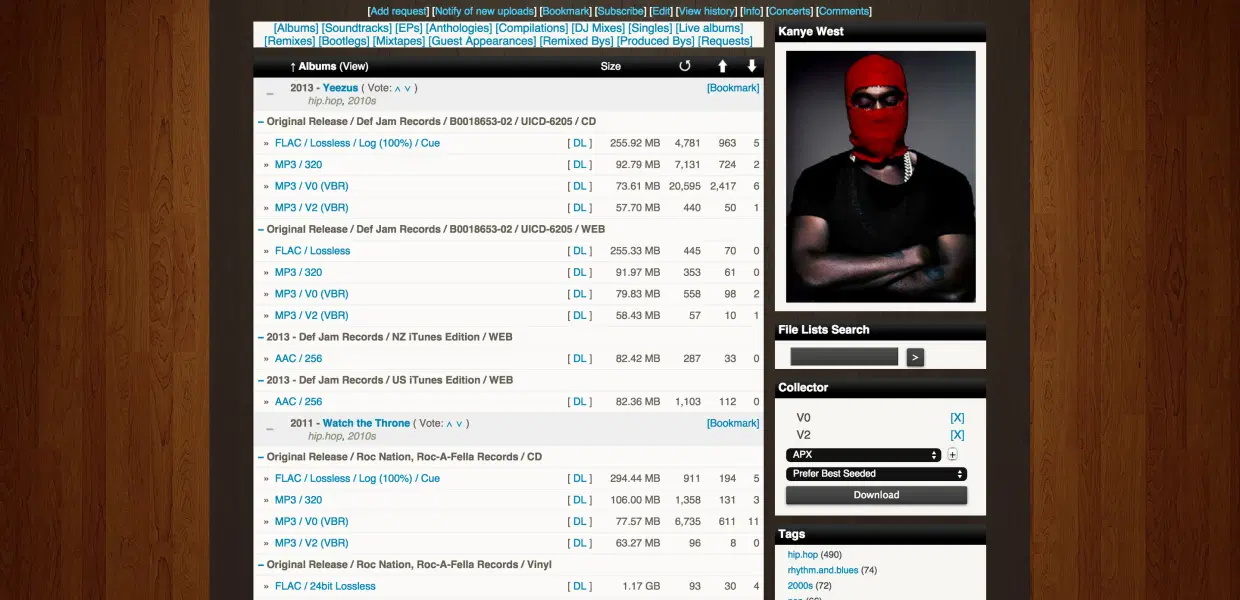
\includegraphics[width=\linewidth]{./images/kanye-what.png}
\label{fig:whatcd} 
\caption{The
what.cd artist page for Kanye West (taken from
\href{https://qz.com/840661/what-cd-is-gone-a-eulogy-for-the-greatest-music-collection-in-the-world/}{here}
in the style of pirates, without permission). For the album ``Yeezus,''
there are ten torrents, grouped by each time the album was released on
CD and Web, and in multiple different qualities and formats (.flac,
.mp3). Along the top is a list of the macro-level groups, where what is
in view is the ``albums'' section, there are also sections for bootleg
recordings, remixes, live albums, etc.}
\end{figure*}

What.cd was a ``private'' bittorrent tracker, where unlike public
trackers that anyone can access, membership was strictly limited to
those who were personally invited or to those who passed an interview
(for more on public and private trackers, see \citep{meulpolderPublicPrivateBitTorrent}). Invites were extremely rare,
and the interview process was demanding to the point where
\href{https://opentrackers.org/whatinterviewprep.com/index.html}{extensive
guides} were written to prepare for them.

The what.cd incentive system was based on a required ratio of data
uploaded vs.~data downloaded \citep{jiaHowSurviveThrive2013}.
Peer to peer systems need to overcome a free-rider problem where users
might download a torrent (``leeching'') and turn their computer off,
rather than leaving their connection open to share it to others (or,
``seeding''). In order to download additional music, then, one would
have to upload more. Since downloading is highly restricted, and
everyone is trying to upload as much as they can, torrents had a large
number of ``seeders,'' and even rare recordings would be sustained for
years, a pattern common to private trackers \citep{liuUnderstandingImprovingRatio2010}.

The high seeder/leecher ratio made it so it was extremely difficult to
acquire upload credit, so users were additionally incentivized to find
and upload new recordings to the system. What.cd implemented a
``bounty'' system, where users with a large amount of excess upload
credit would be able to offer some of it to whoever was able to upload
the album they wanted. To ``prime the pump'' and keep the economy
moving, highlight artists in an album of the week, or direct users to
preserve rare recordings, moderators would also use a ``freeleech''
system, where users would be able to download a specified set of
torrents without it counting against their download quantity \citep{kashEconomicsBitTorrentCommunities2012, chenImprovingSustainabilityPrivate2011a}.

The other half of what.cd was the more explicitly social elements: its
forums, comment sections, and moderation systems. The forum was home to
roiling debates that lasted years about the structure of some tagging
schema, whether one genre was just another with a different name, and so
on. The structure of the community was an object of constant, public
negotiation, and over time the metadata system evolved to be able to
support a library of the entirety of human musical culture\sidenote{Though
  music metadata might seem like a trivial problem (just look at the
  fields in an MP3 header), the number of edge cases are profound. How
  would you categorize an early Madlib cassette mixtape remastered and
  uploaded to his website where he is mumbling to himself while
  recording some live show performed by multiple artists, but on the
  b-side is one of his Beat Konducta collections that mix together
  studio recordings from a collection of other artists? Who is the
  artist? How would you even identify the unnamed artists in the live
  show? Is that a compilation or a bootleg? Is it a cassette rip, a
  remaster, or a web release?}. To support the good operation of the
site, the forums were also home to a huge amount of technical knowledge,
like guides on how to make a perfect copy of a CD or how to detect a
fake upload, that eased new users into being able to use and contribute
to the system.

A critical problem in maintaining coherent databases is correcting
metadata errors and departures from schemas. Finding errors was
rewarded. Users were able to discuss and ask questions of the uploader
in a comment section below each upload, which would allow ``polite''
resolution of low-level errors like typos. More serious problems could
be reported to the moderation team, which caused the upload to be
visibly marked as under review, and the report could then be discussed
either in the comment sections or the forum. The system wasn't perfect:
being an anonymous, gray-area community, there was of course plenty of
power to be abused. Rather than being a messy hodgepodge of fake,
low-quality uploads, though, what.cd was always teetering just shy of
perfection.

These structural considerations do not capture the most elusive but
indisputably important feature of what.cd's community infrastructure:
\emph{the sense of community}. The What.cd forums were the center of
many user's relationships to music. Threads about all the finest scales
of music nichery could last for years: it was a rare place people who
probably cared a little bit too much about music could talk to people
with the same condition. What made it more satisfying than other music
forums was that no matter what music you were talking about, everyone
else in the conversation would always have access to it if they wanted
to hear it. Beyond any structural incentives, people spent so much time
building and maintaining what.cd because it became a source of community
and a sink of personal investment.

Structural norms supported by social systems converge as a sort of
\emph{reputational} incentive. Uploading a new album to fill a bounty
both makes the network more functional and complete, but also
\emph{people respect you for it} because it's prominently displayed on
your profile as well as in the bounty charts and that \emph{feels good}.
Becoming known on the forums for answering questions, writing guides, or
even just having a good taste in music \emph{feels good} and also
contributes to the overall health of the system. Though there are plenty
of databases, and even plenty of different communication venues for
scientists, there aren't any databases (to my knowledge) with integrated
community systems.

The tracker overlay model mirrors and extends some of the
recommendations made by Benedikt Fecher and colleagues in their work on
the reputational economy surrounding data sharing \citep{fecherReputationEconomyHow2017}. They give three policy
recommendations: Increasing reputational benefits, reducing transaction
costs, and ``increasing market transparency by making open access to
research data more visible to members of the research community.'' One
way to accomplish implement them is to embed a data sharing system
within a social system that is designed to reward communitarian
behavior.

Many features of what.cd's structure are undesirable for scientific
infrastructure, but they demonstrate that a robust archive is not only a
matter of building a database with some frontend, but also building a
community \citep{brossCommunityCollaborationContribution2013}. Of
course, we need to be careful with building the structural incentives
for a data sharing system: the very last thing we want is another
\href{https://etiennelebel.com/cs/t-leaderboard/t-leaderboard.html}{coercive
leaderboard} that turns what should be a collaborative effort punitive.
In contrast to what.cd, for infrastructure we want extremely low
barriers to entry, and be agnostic to resources --- researchers with
access to huge server farms should not be unduly favored. We should
think carefully about using downloading as the ``cost,'' because
downloading and analyzing huge amounts of data can be \emph{good} and
exactly what we \emph{want} in some circumstances, but a threat to
privacy and data governance in others.

This model has its own problems, including the lack of interoperability
between different trackers, the need to recreate a new set of accounts
and database for each new tracker, among others. It's also been tried
before: sharing data in specific formats (as our running example,
Neurodata Without Borders) on indexing systems like bittorrent trackers
amounts to something like BioTorrents \citep{langilleBioTorrentsFileSharing2010}  or
\href{https://academictorrents.com/}{AcademicTorrents} \citep{cohenAcademicTorrentsCommunityMaintained2014}. Even with our
extensions of version control and some model of automatic mirroring of
data across the network, we still have some work to do. To address these
and several other remaining needs for scientific data infrastructure, we
can take inspiration from \emph{federated systems.}

\hypertarget{linked-data-or-surveillance-capitalism}{%
\subsection{Linked Data or Surveillance
Capitalism?}\label{linked-data-or-surveillance-capitalism}}

\begin{leftbar}
Having become a dense and consistent historical reality, language forms
the locus of tradition, of the unspoken habits of thought, of what lies
hidden in a people's mind; it accumulates an ineluctable memory which
does not even know itself as memory. Expressing their thoughts in words
of which they are not the masters, enclosing them in verbal forms whose
historical dimensions they are unaware of, men believe that their speech
is their servant and do not realize that they are submitting themselves
to its demands.

Michel Foucault --- \emph{The Order of Things} \citep{foucaultOrderThings2001} 
\end{leftbar}

There is no shortage of databases for scientific data, but their
traditional structure chokes on the complexity of representing
multi-domain data. Typical relational databases require some formal
schema to structure the data they contain, which have varying
reflections in the APIs used to access them and interfaces built atop
them. This broadly polarizes database design into domain-specific and
domain-general\sidenote{To continue the analogy to bittorrent trackers,
  an example domain-specific vs.~domain-general dichotomy might be
  What.cd (with its specific formatting and aggregation tools for
  representing artists, albums, collections, genres, and so on)
  vs.~ThePirateBay (with its general categories of content and otherwise
  search-based aggregation interface)}. This design pattern results in a
fragmented landscape of databases with limited interoperability. How
shall we link the databases? In this section we'll consider the Icarian
promise of creating the great unified database of everything as a way of
motivating an alternative that blends \emph{linked data} \citep{berners-leeLinkedData2006}  with \emph{federated systems} against our
peer to peer backbone in the next section.

Domain-specific databases require data to be in one or a few specific
formats, and usually provide richer tools for manipulating and querying
by metadata, visualization, summarization, aggregation that are
purpose-built for that type of data. For example, NIH's
\href{https://www.ncbi.nlm.nih.gov/gene/12550}{Gene} tool has several
visualization tools and cross-referencing tools for finding expression
pathways, genetic interactions, and related sequences (Figure xx). This
pattern of database design is reflected at several different scales,
through institutional databases and tools like the Allen
\href{https://connectivity.brain-map.org/}{brain atlases} or
\href{http://observatory.brain-map.org/visualcoding/}{observatory}, to
lab- and project-specific dashboards. This type of database is natural,
expressive, and powerful --- for the researchers they are designed for.
While some of these databases allow open data submission, they often
require explicit moderation and approval to maintain the guaranteed
consistency of the database, which can hamper mass use.

\begin{figure*}
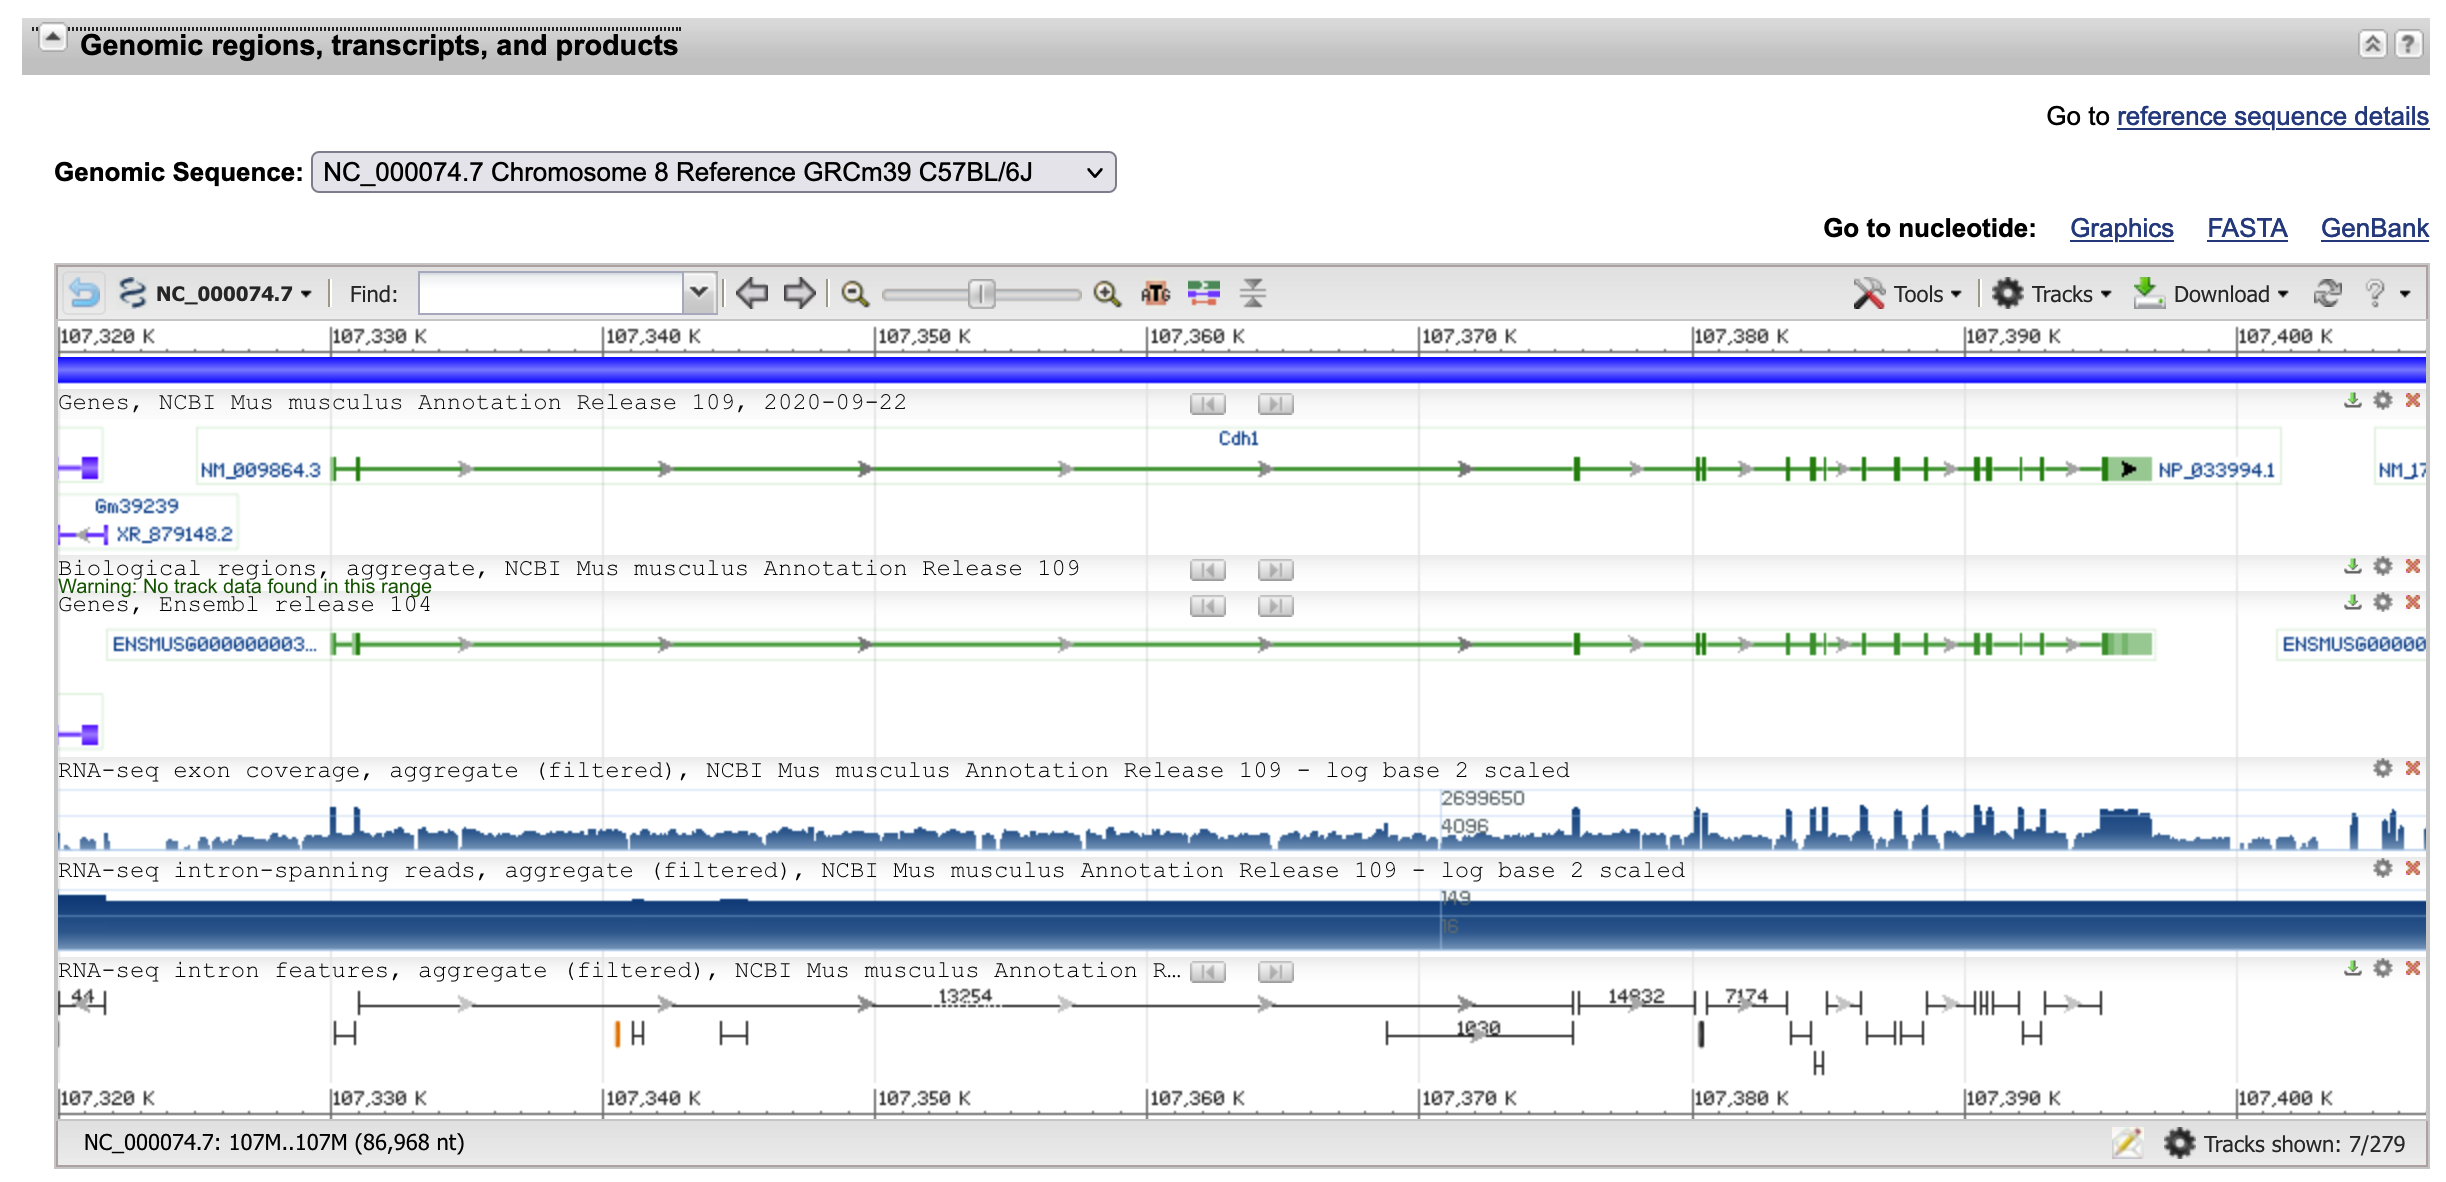
\includegraphics[width=\linewidth]{./images/nih_gene_cdh1.png}
\label{fig:genetool}
\caption{NIH's Gene tool includes many specific tools for visualizing,
cross-referencing, and aggregating genetic data. Shown is the ``genomic
regions, transcripts, and product'' plot for Mouse Cdh1, which gives
useful, common summary descriptions of the gene, but is not useful for,
say, visualizing reading proficiency data from educational research.}
\end{figure*}

General-purpose databases like \href{https://figshare.com/}{figshare}
and \href{https://zenodo.org/}{zenodo}\sidenote{No shade to Figshare,
  which, among others, paved the way for open data and are a massively
  useful thing to have in society.} are useful for the mass aggregation
of data, typically allowing uploads from most people with minimal
barriers. Their general function limits the metadata, visualization, and
other tools that are offered by domain-specific databases, however, and
are essentially public, versioned, folders with a DOI. Most have fields
for authorship, research groups, related publications, and a
single-dimension keyword or tags system, and so don't programmatically
reflect the metadata present in a given dataset.

The dichotomy of fragmented, subdomain-specific databases and
general-purpose databases makes combining information from across even
extremely similar subdisciplines combinatorically complex and laborious.
In the absence of a formal interoperability and indexing protocol
between databases, even \emph{finding} the correct subdomain-specific
database often comes down to pure luck. It also puts researchers who
want to be good data stewards in a difficult position: they can hunt
down the appropriate subdomain specific database and risk general
obscurity; use a domain-general database and make their work more
difficult for themselves and their peers to use; or spend all the time
it takes to upload to multiple databases with potentially conflicting
demands on format.

What can be done? There are a few naïve answers from standardizing
different parts of the process: If we had a universal data format, then
interoperability becomes trivial. Conversely, we could make a single
ur-database that supports all possible formats and tools.

The notion of a universal database system almost immediately runs
aground on the reality that organizing knowledge is intrinsically
political. Every subdiscipline has conflicting \emph{representational}
needs, will develop different local terminology, allocate differing
granularity and develop different groupings and hierarchies for the same
phenomena. At their mildest, differences in representational systems can
be incompatible, but at their worst they can reflect and reinforce
prejudices and become the site of expression for intellectual and social
power struggles \citep{joLessonsArchivesStrategies2020, selbstFairnessAbstractionSociotechnical2019, gebruDatasheetsDatasets2021, bowkerSortingThingsOut1999}. Every subdiscipline has conflicting
\emph{practical} needs, with infinite variation in privacy demands,
different priorities between storage space, bandwidth, and computational
power, and so on. In all cases the boundaries of our myopia are
impossible to gauge: we might think we have arrived at a suitable schema
for biology, chemistry, and physics\ldots{} but what about the
historians?

Matthew J Bietz and Charlotte P Lee articulate this tension in their
ethnography of metagenomics databases:

\begin{leftbar}
``Participants describe the individual sequence database systems as if
they were shadows, poor representations of a widely-agreed-upon ideal.
We find, however, that by looking across the landscape of databases, a
different picture emerges. Instead, \textbf{each decision about the
implementation of a particular database system plants a stake for a
community boundary. The databases are not so much imperfect copies of an
ideal as they are arguments about what the ideal Database should be.}
{[}\ldots{]}

In the end, however, \textbf{the system was so tailored to a specific
set of research questions that the collection of data, the set of tools,
and even the social organization of the project had to be significantly
changed.} New analysis tools were developed and old tools were
discarded. Not only was the database ported to a different technology,
the data itself was significantly restructured to fit the new tools and
approaches. While the database development projects had begun by working
together, in the end they were unable to collaborate. \textbf{The system
that was supposed to tie these groups together could not be shielded
from the controversies that formed the boundaries between the
communities of practice.}'' \citep{bietzCollaborationMetagenomicsSequence2009} 
\end{leftbar}

The pursuit of unified representation is an intimate part of the history
of linked data, which relies on ``ontologies'' or controlled
vocabularies that describe a set of objects (or classes) and the
properties they can have. For example,
\href{https://schema.org}{schema.org} maintains a widely used set of
hierarchical vocabularies to describe the fundamental things that exist
in the world, in particular the unfamiliar world in which a
\href{https://schema.org/Person}{Person} has a
\href{https://schema.org/gender}{gender} and
\href{https://schema.org/netWorth}{net worth} but lacks a race \citep{poirierTurnScruffyEthnographic2017}. At one extreme in the world of
ontology builders, the ideological nature of demarcating what is allowed
to exist is as clear as a klaxon (emphasis in original):

\begin{leftbar}
An exception is the Open Biomedical Ontologies (OBO) Foundry initiative,
which accepts under its label only those ontologies that adhere to the
principles of ontological realism. {[}\ldots{]} Ontologies, from this
perspective, are representational artifacts, comprising a taxonomy as
their central backbone, whose representational units are intended to
designate \emph{universals} (such as \emph{human being} and
\emph{patient role}) or \emph{classes defined in terms of universals}
(such as \emph{patient,} a class encompassing \emph{human beings} in
which there inheres a \emph{patient role}) and certain relations between
them. {[}\ldots{]}

BFO is a realist ontology {[}15,16{]}. This means, most importantly,
that representations faithful to BFO can acknowledge only those entities
which exist in (for example, biological) reality; thus they must reject
all those types of putative negative entities - lacks, absences,
non-existents, possibilia, and the like \citep{ceustersFoundationsRealistOntology2010} 
\end{leftbar}

In practice, because of the difficulty of changing the representation
and encompassing database systems on a dime, using these ontologies to
link disparate datasets tends to follow the pattern of metadata
\emph{overlays} where the structure of individual databases are mapped
onto one ``unifying'' ontology to allow for aggregation and translation.
This approach appears gentler than standardization at the level of
individual databases, but has the same problems kicked up one level of
abstraction.

To concretize the problems with a globally unified database or metadata
overlay, the remainder of this section will trace the compromises and
outcomes of the The NIH's ``Biomedical Data Translator'' project\sidenote[][-3.25cm]{A conversation with someone close to the project just before the initial publication of this piece made clear several changes that need to be made to this section, but prevailing circumstances in academic publishing hastened its release before I could make them. I intend this section as good-faith criticism of a lot of hard work by researchers who I assume are working with the best intentions, and invite comment and clarification from anyone working within the Translator project for revisions in a future version.}. The
Translator project was initially described in the 2016 Strategic Plan
for Data Science as a means of translating between biomedical data
formats:

\begin{leftbar}
Through its Biomedical Data Translator program, the National Center for
Advancing Translational Sciences (NCATS) is supporting research to
develop ways to connect conventionally separated data types to one
another to make them more useful for researchers and the public. \citep{NIHStrategicPlan2018} 
\end{leftbar}

The original
\href{https://web.archive.org/web/20210709100523/https://ncats.nih.gov/news/releases/2016/feasibility-assessment-translator}{funding
statement from 2016} is similarly humble, and press releases
\href{https://web.archive.org/web/20210709171335/https://ncats.nih.gov/pubs/features/translator}{through
2017} also speak mostly in terms of querying the data -- though some
ambition begins to creep in. By 2019, the vision for the project had
veered sharply away from anything a basic researcher might recognize as
a means of translating between data types. In their piece ``Toward a
Universal Biomedical Translator,'' then in a feasibility assessment
phase, the members of the Translator Consortium assert that universal
translation between biomedical data is impossible \citep{consortiumUniversalBiomedicalData2019}. The
impossibility they saw was not that of conflicting political demands on
the structure of organization (as per \citep{bowkerSortingThingsOut1999}), but of the sheer numeracy of the data
and vocabularies needed to describe them. The risk posed by a lack of a
universal ``language'' was not being able to index all possible data,
rather than inaccuracy or inequity.

Undaunted by their stated belief in the impossibility of a
universalizing ontology, the Consortium created one in their
\href{https://biolink.github.io/biolink-model/docs/}{biolink} model \citep{bruskiewichBiolinkBiolinkmodel2021, unniBiolinkModelUniversal2022}. Biolink consists of a hierarchy of basic classes: eg. a
\href{https://biolink.github.io/biolink-model/docs/BiologicalEntity.html}{BiologicalEntity}
like a
\href{https://biolink.github.io/biolink-model/docs/Gene.html}{Gene}, or
a
\href{https://biolink.github.io/biolink-model/docs/ChemicalEntity.html}{ChemicalEntity}
like a
\href{https://biolink.github.io/biolink-model/docs/Drug.html}{Drug}.
Classes can then linked by any number of properties, or ``Slots,'' like
a therapeutic procedure that
\href{https://biolink.github.io/biolink-model/docs/treats.html}{treats}
a disease.

The translator does not attempt to respond to the needs of researchers
or labs who might want to link their raw data splayed out across flash
drives and file structures whose chaos borders on whimsy. Instead, the
Translator operates at the level of ``knowledge,'' or ``generally
accepted, universal assertions derived from the accumulation of
information'' \citep{fechoProgressUniversalBiomedical2022}.
Rather than translating \emph{between data types}, the meaning of
``translation'' shifted to meaning \emph{``translating data into
knowledge''} \citep{consortiumUniversalBiomedicalData2019}.

To feed the Translator, Biolink sits ``on top of'' a
\href{http://www.smart-api.info/registry}{collection of database APIs}
that serve structured biomedical data, each called a ``knowledge
source.'' Individual APIs
\href{https://github.com/NCATSTranslator/ReasonerAPI}{declare} that they
are able to provide data for a particular set of classes or slots, like
\href{http://www.smart-api.info/ui/adf20dd6ff23dfe18e8e012bde686e31}{drugs
that affect genetic expression}, and are then made browsable from the
\href{http://www.smart-api.info/portal/translator/metakg}{SmartAPI
Knowledge Graph}. Queries to individual APIs do not return ``raw'' data,
but return assertions of fact in the parlance of the Biolink model: this
procedure treats that disease, etc.

Because individual researchers do not typically represent their data in
the form of factual assertions, knowledge sources are constrained to
``highly curated biomedical databases'' or other aggregated systems. The
NIH RePORTER tool
\href{https://reporter.nih.gov/search/DShVUhB_ZUq0X5UWFjy5WQ/projects?shared=true}{gives
an overview} of the way these knowledge sources are prepared when none
already exist for a given Biolink class or predicate: automated
\href{https://reporter.nih.gov/project-details/10548337}{text mining}
tools and a series of
\href{https://reporter.nih.gov/project-details/10056962}{domain-specific
data provider} projects, rather than via tools provided to researchers.

The collection of knowledge sources, linked to nodes and edges in the
Biolink model, are designed to be queried as a graph. To answer a query
like ``what drug treats this disease?'' the translator considers the
graph of entities linked to the disease: what symptoms does the disease
have? what genes are linked to those symptoms? which drugs act on those
genes? and so on \citep{renaissancecomputinginstituterenciBiomedicalDataTranslator2022}. The
form of the Translator as a graph-based question answering machine
bounds its application as a platform for researchers to guide their
research and clinicians to guide their care \citep{hailuNIHfundedProjectAims2019}, rather than a tool for linking data.

One primary example currently featured by NCATS is using the translator
to propose novel treatments for drug-induced liver injury (DILI) \citep{renaissancecomputinginstituterenciUseCasesShow2022}  detailed in
a 2021 conference paper \citep{goelExplanationContainerCaseBased2021}. To find a candidate drug, the researchers manually conducted three
API queries: first they searched for phenotypes associated with DILI and
selected ``one of them''\sidenote{Using the only API listed with a
  ``related to'' link between disease and phenotypic feature,
  \href{https://smart-api.info/ui/1d288b3a3caf75d541ffaae3aab386c8}{SEMMEDDB},
  I was unable to find ``Red blood cell count'' with DILI (C0860207) as
  either the
  \href{https://biothings.ncats.io/semmeddb/query?q=subject.umls\%3AC0860207\&facet_size=10\&fetch_all=true\&_sorted=true\&format=json}{subject}
  or
  \href{https://biothings.ncats.io/semmeddb/query?q=object.umls\%3AC0860207\&facet_size=10\&fetch_all=true\&_sorted=true\&format=json}{object},
  and it is unclear why one would prefer that to any number of other
  phenotypes like ``Fever'' or the ominous symptom named ``Symptoms''
  (C1457887).} --- ``red blood cell count''. Then they queried for genes
associated with red blood cell count to find telomerase reverse
transcriptase (TERT), and then finally for drugs that affect TERT to
find Zidovudine. The directionality of each of these relationships, high
vs.~low, increases vs.~decreases, is unclear in each case. A more recent
report on the Translator repeated this pattern of manual querying,
arriving at a handful of different genes and drugs \citep{fechoProgressUniversalBiomedical2022}.

While the current examples are highly manual, providing an array of
results for each query along with links to associated papers on pubmed,
some algorithmic system for ranking results is necessary to make use of
the information in the extended knowledge graph. Rather than just the
first-order connections, it should be possible to make use of second,
third, and n-th order connections to weight potential results.
Algorithmic medical recommendation systems have been thoroughly
problematized elsewhere (eg. \citep{groteEthicsAlgorithmicDecisionmaking2020, obermeyerDissectingRacialBias2019, panchArtificialIntelligenceAlgorithmic2019, panchInconvenientTruthAI2019}). The primary ranking algorithm is developed by a defense
contractor (CoVar) who has\sidenote{seemingly unironically} named it
ROBOKOP \citep{mortonROBOKOPAbstractionLayer2019} \sidenote{which
  seems totally fine and normal.}. Though ROBOKOP functions with a
simple weighted graph metric based on citations and abstract text, the
ranking system is intended to be extended with machine learning tools
\citep{mortonROBOKOPAbstractionLayer2019}  that can be trained
based on the way the provided answers are used \citep{consortiumUniversalBiomedicalData2019}. Algorithmic recommendation
platforms are in a regulatory gray area \citep{ordishAlgorithmsMedicalDevices2019, el-sayedMedicalAlgorithmsNeed2021}, but would arguably need to have interpretable results with clear
provenance to pass scrutiny. The DILI example uses a language model
which explained the recommendation of Zidovudine with all the clarity of
``one of `DOWNREGULATOR,' `INHIBITOR,' `INDIRECT DOWNREGULATOR'.''

The arrival at a biomedical question answering platform built atop an
algorithmic ranking system for a knowledge graph that queries 200+
aggregated data sources has several qualities that should give us pause.

First, as with any machine-learning based system, the algorithm can only reflect the implicit structure of its creation, including the beliefs and values of its architects \citep{ birhaneValuesEncodedMachine2022, birhaneAlgorithmicInjusticeRelational2021}, its training data and accompanying bias \citep{birhaneMultimodalDatasetsMisogyny2021}, and so on. The ``mass
of data'' approach ML tools lend themselves to, in this case, querying
hundreds of independently operated databases, makes dissecting the
provenance of every entry from every data provider effectively
impossible. For example, one of the providers,
\href{https://mydisease.info}{mydisease.info} was more than happy to
respond to a query for the outmoded definition of ``transsexualism'' as
a disease \citep{ramTransphobiaEncodedExamination2021}  along with
a list of genes and variants that supposedly ``cause'' it -
\href{http://mydisease.info/v1/query?q=\%22DOID\%3A10919\%22}{see for
yourself}. At the time of the search, tracing the source of that entry
first led to the disease ontology
\href{https://web.archive.org/web/20211007053446/https://www.ebi.ac.uk/ols/ontologies/doid/terms?iri=http\%3A\%2F\%2Fpurl.obolibrary.org\%2Fobo\%2FDOID_1234}{DOID:1234}
which traced back into an entry in a graph aggregator
\href{http://www.ontobee.org/ontology/DOID?iri=http://purl.obolibrary.org/obo/DOID_1234}{Ontobee}
(\href{https://web.archive.org/web/20210923110103/http://www.ontobee.org/ontology/DOID?iri=http://purl.obolibrary.org/obo/DOID_1234}{Archive
Link}), which in turn listed this
\href{https://github.com/jannahastings/mental-functioning-ontology}{github
repository} \textbf{maintained by a single person} as its
source\sidenote{I submitted a
  \href{https://github.com/jannahastings/mental-functioning-ontology/pull/8}{pull
  request} to remove it, but it has not been merged more than 8 months
  later. A teardrop in the ocean.}. This is, presumably, the fragility
and inconsistency in input data that the machine learning layer is
intended to putty over.

If the graph encodes being transgender as a disease, it is not
farfetched to imagine the ranking system attempting to ``cure'' it. In a
seemingly prerelease version of the translator's query engine, ARAX, it
does just that: in
\href{https://arax.rtx.ai/?r=e891e6e6-44fd-4684-9d36-f94e3e81b554}{a
query for entities with a \texttt{biolink:treats} link to gender
dysphoria}\sidenote{To its credit, ARAX does transform the request for
  \texttt{DOID:10919} to \texttt{MONDO:0001153} - gender dysphoria.}, it
ranks the standard therapeutics \citep{deutschOverviewFeminizingHormone2016, deutschOverviewMasculinizingHormone2016}  Testosterone and Estradiol
6th and 10th of 11, respectively --- behind a recommendation for Lithium
(4th) and Pimozide (5th) due to an automated text scrape of
\href{https://pubmed.ncbi.nlm.nih.gov/2114800/}{two} conversion therapy
\href{https://pubmed.ncbi.nlm.nih.gov/8839957/}{papers}. \sidenote{as well
  as a recommendation for ``date allergenic extract'' from a
  misinterpretation of ``to date'' in the abstract of
  \href{https://pubmed.ncbi.nlm.nih.gov/24330520/}{a paper} that reads
  ``Cross-sex hormonal treatment (CHT) used for gender dysphoria (GD)
  could by itself affect well-being without the use of genital surgery;
  however, \textbf{to date,} there is a paucity of studies investigating
  the effects of CHT alone''}. Queries to ARAX for
treatments for \href{https://arax.ncats.io/?r=52703}{gender identity
disorder} helpfully yielded ``zinc'' and ``water,'' offering a paper
from the translator group that describes automated drug recommendation
as the only provenance \citep{womackLeveragingDistributedBiomedical2019}. A query for treatments
for \texttt{DOID:1233}
``\href{https://arax.rtx.ai/?r=81249a42-b300-4dcf-94c9-7a9fe2f78237}{transvestism}''
was predictably troubling.

Even if the curators do their best to prevent harmful queries and block
searches for ``cures'' to being trans, the graph-based nature of the
system means that any given entry will have unpredictable consequences
on recommendations made from the surrounding network of objects like
genes, treatment history, and so on. If the operation of the ranking
algorithm is uninterpretable, as most are, or the algorithm it itself
proprietary, harmful input data could have long-range influence on both
the practice of medicine as well as the course of basic research
\emph{without anyone being able to tell.} The Consortium also describes
a system whereby the algorithm is continuously updated based on usage of
results in research or clinical practice \citep{consortiumUniversalBiomedicalData2019}, which stands to magnify the
problem of algorithmic bias by uncritically treating harmful treatment
and research practices as training data.

The approach creates a fundamental tradeoff between algorithmic
interpretability and the system being useful at all. The paper cited in
the 2021 DILI example as evidence that the system gives plausible
results is for a specific subclass of liver injuries caused by
anti-tuberculosis drugs \citep{udomsinprasertLeukocyteTelomereLength2020}, highlighting the danger
of automated recommendations from noisy data, but also calling into
question what novel contribution the Translator made if telomeres were
already implicated in DILI. The 2022 report gives examples where the
results were already expected by the researchers, or provided a series
of papers that seems difficult to imagine being much more informative
than a PubMed search. If the algorithmic recommendations are unexpected
--- ie. the system provides novel information --- the process of
confirming them appears to be near-identical to the usual process of
reading abstracts and hopping citation trees.

Perhaps most worrisome is the eventual fate of the project in the hands
of the broader ecosystem of orbiting information conglomerates.
Centralized infrastructure projects can be an opportunity for for-profit
companies to ``dance until the music stops'' and then scoop up any
remaining technology when the funding dries up (so far roughly
\href{https://reporter.nih.gov/search/kDJ97zGUFEaIBIltUmyd_Q/projects?sort_field=FiscalYear\&sort_order=desc}{\$81.6
million} since 2016 for the Translator \citep{RePORTRePORTERBiomedical2021}, and
\href{https://reporter.nih.gov/search/H4LxgMGK9kGw6SeWCom85Q/projects?shared=true}{\$84.7
million} for the discontinued NIH Data Commons pilot which morphed into
the STRIDES program). I have little doubt that the scientists and
engineers working on the Translator are doing so with the best of
intentions --- the real question is what happens to it after it's
finished.

Knowledge graphs in particular are promising targets for platform
holders. Perhaps the most well known example is Google's 2010
acquisition of Freebase (via Metaweb) \citep{subramanianGoogleBuysFreebase2010}, a graph of structured data with
a wealth of properties for common people, places and things. Google
incorporated it into their Knowledge Graph \citep{IntroducingKnowledgeGraph2012}  to populate its factboxes and make
its search results more semantically aware in its Hummingbird upgrade in
2013, the largest overhaul of its search engine since 2001 \citep{sullivanFAQAllNew2013}, cementing its dominance as a search engine.
The connection between swallowing up knowledge organization systems into
search engines is not incidental, but reflective of the broader pattern
of enclosing basic digital infrastructure behind opaque platforms.
Searching has a different set of cognitive expectations than browsing a
database: we expect search results to be ``best effort,'' not
necessarily complete or accurate, where when browsing a database it's
relatively clear when information is missing or inaccurate. For products
packaged up into search platforms by for-profit companies, \emph{it
doesn't have to actually work} as long as it seems like it does.

The platformatization of the knowledge graph, along with carefully
worded terms of service, is a clean means by which ``good enough''
results could be jackknifed into an expanded system of biomedical
surveillance. Since the algorithm needs continual training, the
translator has every incentive to suck up as much personal data as it
can\sidenote{A 2020 presentation in one of the Translator's
  \href{https://github.com/NCATSTranslator/Translator-All}{github
  repositories} describes methods for mining individual clinical data
  \citep{translatorconsortiumClinicalDataServices2020} }.
For-profit platform providers as a rule depend on developing elaborate
personal profiles for targeted advertising algorithmically inferred from
available data\sidenote{A patent from Google is telling about how they
  view privacy concerns: whatever we can't get explicitly, we'll infer
  to sell better ads! \\ "One possible method to improve ad
  targeting is for ad targeting systems to obtain and use user profiles.
  For example, user profiles may be determined using information
  voluntarily given by users (e.g., when they subscribe to a service).
  This user attribute information may then be matched against advertiser
  specified attributes of the ad (e.g., targeting criteria).
  Unfortunately, user profile information is not always available since
  many Websites (e.g., search engines) do not require subscription or
  user registration. Moreover, even when available, the user profile may
  be incomplete (e.g., because the information given at the time of
  subscription may be limited to what is needed for the service and
  hence not comprehensive, because of privacy considerations, etc.).
  Furthermore, advertisers may need to manually define user profile
  targeting information. In addition, even if user profile information
  is available, advertisers may not be able to use this information to
  target ads effectively." \citep{bharatGeneratingUserInformation2005} }, that naturally includes diagnosed or inferred disease --- a
practice they explicitly describe in the patents for the targeting
technology \citep{bharatGeneratingUserInformation2005}, have gone
to court to defend \citep{SmithFacebookInc2018, krashinskyGoogleBrokeCanada2014}, and formed secretive joint
projects with healthcare systems to pursue \citep{bourreauGoogleFitbitWill2020}.

So while an algorithmic recommendation tool may have limited use for the
basic researchers it was originally intended for, it is likely to be
extremely useful for the booming business of ``personalized medicine.\sidenote{The researchers in the Translator project are clear that they do not intend it as a tool for personalized medicine, but again we are describing unintended downstream consequences by different actors than the creators.}''
Linking biomedical and patient data in a single platform is a natural
route towards a multisided market where records management apps are sold
to patients, treatment recommendation systems are sold to clinicians,
research tools and advertising opportunities are sold to pharmaceutical
companies, risk metrics are sold to insurance companies, and so on.

Multiple information conglomerates are poised to capitalize on the
translator project. Amazon already has a broad home surveillance
portfolio \citep{bridgesAmazonRingLargest2021}, and has been
aggressively expanding into health technology \citep{AWSAnnouncesAWS2021}  and even literally providing
\href{https://amazon.care/}{health care} \citep{lermanAmazonBuiltIts2021}, which could be particularly dangerous
with the uploading of all scientific and medical data onto AWS with
entirely unenforceable promises of data privacy through NIH's STRIDES
program \citep{quinnYouCanTrust2021}.

RELX, parent of Elsevier, is as always the terrifying elephant in the
room. In addition to distribution rights for a large proportion of
scientific knowledge and a collection of research databases, it also
sells a clinical reference platform in ClinicalKey, point of service
products for planning patient care with ClinicalPath, medical education
tools, and pharmaceutical advertisements designed to look like
scientific papers \citep{elsevier360AdvertisingSolutions}, among
others \citep{relx2021AnnualReport2021}. It also is explicitly
expanding into ``clinical decision support applications'' \citep{relx2021AnnualReport2021}  and recently embedded its medication
management product into Apple's watchOS 9 \citep{appleWatchOSDeliversNew2022}. Subsidiaries in RELX's ``Risk'' market
segment sell risk profiles to insurance companies based on what they
claim to be highly comprehensive profiles of harvested personal data.
The Translator infrastructure is a perfect keystone to unify these
products: after the NIH fronts the money to develop it and lends the
credibility of basic research, RELX can cheaply expand its surveillance
apparatus to enhanced medical risk profiles to insurers, priority
placement in candidate drug rankings to pharmaceutical companies, and
augment its ranking systems for funders and employers to include some
proprietary metric of ``promisingness'' to encourage researchers to
follow its research recommendations. This isn't speculative --- it can
just strap whatever clinical data Translator gains access to into its
\href{https://www.elsevier.com/solutions/biology-knowledge-graph}{existing
biomedical knowledge graph}.

Even assuming the Translator works perfectly and has zero unanticipated
consequences, the development strategy still reflects the inequities
that pervade science rather than challenge them. Biopharmaceutical
research, followed by broader biomedical research, being immediately and
extremely profitable, attracts an enormous quantity of resources and
develops state of the art infrastructure, while no similar
infrastructure is built for the rest of science, academia, and society.

The eventual form of the Translator follows from a series of decisions
centered around the intended universality of the system. From the
\href{https://web.archive.org/web/20210709100523/https://ncats.nih.gov/news/releases/2016/feasibility-assessment-translator}{funding
statement} in 2016, the system was conceptualized as an ``informatics
platform'' intended to ``bring together all biomedical and health data
types.'' The surrounding background of cloud-based database storage
imagined by the Strategic Plan for Data Science immediately constrained
the design to consist of APIs that served small quantities of aggregated
data, rather than potentially large quantities of raw data. Together
with a platform, rather than tool-based approach, a system that allowed
individual researchers to link and make sense of the subtlety of own
their data was precluded from the start.

From these constraints, the form of the BioLink model comes into focus:
high-level classes and logical relationships between them as asserted by
a large number of separate knowledge sources. Since the data from each
of these sources is heterogeneous, relatively uncurated, and potentially
numerous for any given graph-based query, the need for a machine
learning layer to make sense of it follows. The conceptualization of
BioLink as a universal ontology seems to follow the lineage of the
``neat'' thought style \citep{poirierTurnScruffyEthnographic2017} 
that emphasizes ``deductive inference through logical rules'' \citep{unniBiolinkModelUniversal2022}  or otherwise computing derived
information from the structure of the knowledge graph rather than
browsing the graph itself. Together, these constraints and design logics
bring us to the form of the Translator as a graph-based query engine.

The Translator Consortium justifiably takes pride in its social
organizing systems \citep{consortiumBiomedicalDataTranslator2019} 
--- coordinating 200 researchers and engineers from dozens of
institutions is no small feat. This system of social organization seems
to have lent itself towards developing the individual components with an
eye for them to be understood by the rest of the \emph{consortium}
rather than with the intention of inviting collaboration from the
broader research community\sidenote{The descriptions of difficulty in
  interfacing the components of the project internally are littered
  throughout their public-facing documents: eg. ``A lot of the work has
  been about defining standards, so that the components that each of the
  15 teams are building can talk to each other'' \citep{renaissancecomputinginstituterenciBiomedicalDataTranslator2022},
  ``In part due to the speed with which the program has progressed, team
  members also have found it challenging to coordinate milestones and
  deliverables across teams and align the goals of the Translator
  program with the goals of their own nonTranslator research projects.''
  \citep{consortiumBiomedicalDataTranslator2019}. These problems
  are, of course, completely reasonable. My comment here merely suggests
  that solving these problems, particularly on the self-described tight
  timeline of the Translator's development, may have edged out concerns
  for engagemenent with the broader research community.}. The very
notion of a platform indicates that it is something that \emph{they
build} and \emph{we use}: There is no explicit means for proposing
changes to the BioLink model, to pick and choose how answers are ranked
or queries are performed, etc. This is broadly true of platform-based
scientific tools, especially databases, and contributes to how they
\emph{feel}: they feel disconnected with our work, don't necessarily
help us do it more easily or more effectively, and contributing to them
is a burdensome act of charity (if it is possible at all).

Given the real need for \emph{some} means of combining heterogeneous
data from disparate sources, what could have been done differently?

Problematizing the need for a system intended to link \emph{all} or even
\emph{most} biomedical data in a single mutually coherent system opens
the possibility for a very different data linking infrastructure.
Perhaps paradoxically, any universal, logically complete schema intended
to support algorithmic inference projects a relatively circumscribed
group of people for whom it would be useful: nearly all of the publicly
described use-cases are oriented around finding new drugs or targets to
treat disease, presumably in part because that's what preoccupies the
ontology. Rather than a set of generalizable \emph{tools} for linking
data, the need for universality strongly constrains the form of data
that can be represented by the system, and its platform structure
constrains its uses to only those imagined by the platform designers.
Every infrastructural model is an act of balancing constraints, and
prioritizing ``all data'' seems to imply ``for some people.'' Who is
supposed to be able to upload data? change the ontology? inspect the
machine learning model? Who is in charge of what? Who is a
knowledge-graph query engine useful for?

Another conceptualization might be building systems for \emph{all
people} that can \emph{embed with existing practices} and \emph{help
them do their work} which typically involves accessing \emph{some data.}
We can imagine a system designed to integrate data with schemas written
in the \emph{vernacular} of communities of knowledge work. Rather than
the dichotomy of one singular database vs.~many fragmented and
incompatible databases, we can imagine a \emph{pluralistic} system
capable of supporting multiple overlapping and potentially conflicting
representations, governable and malleable in local communities of
practice. Taking seriously the notion of ``translation,'' we could stand
to learn from linguistics and translation studies: rather than
attempting to project the dialects of each subdiscipline into some
``true'' meta-framework (a decidedly colonial project \citep{shammaTranslationColonialism2018}), we could resist the urge for
homogenization and preserve the multiplicity of representation,
embracing the imperfection of mappings between heterogeneous
representational systems at multiple scales without resigning ourselves
to completely isolated incompatibility.

Maybe we don't \emph{want} a universal system that presents itself with
the authority of truth to be mined and spun off into derivative
platforms by information conglomerates. We might abandon the
techno-utopianism of a globally consistent schema that supports
arbitrary logical inference by acknowledging that those inferences would
always be colored by the decisions embedded in the structure of the
system, unknowable beneath the shrouding weights of its ranking model.

Instead can we imagine a properly \emph{human} data infrastructure? One
that preserves the seams and imperfections in our representational
systems, that is designed to represent precisely the contingency of
representation itself? (eg. see \citep{birhaneImpossibilityAutomatingAmbiguity2021, fletcher-watsonDiversityComputing2018}). We might start with the propositional nature of
links and mappings between formats --- that rather than a divine
received truth, the relationships between things are contextual and
created. We could find grounding in \emph{use,} that the schemas and
mappings between them should arise from the need to link representations
within the context of some problem, rather than to resolve their
difference.

Picking up the thread of our peer to peer data sharing backbone, we
might start to imagine the boistrous multiplicity of an infrastructure
based around communication and expression, rather than platformatized
perfection.

\hypertarget{folk-federation}{%
\subsection{Folk Federation}\label{folk-federation}}

\begin{leftbar}
Human language thrives when using the same term to mean somewhat
different things, but automation does not. \emph{Tim Berners-Lee (1999)
The Semantic Web} \citep{berners-leeSemanticWeb2001} 
\end{leftbar}

\begin{leftbar}
Wittgenstein's contribution to communism was his robust proof of the
proposition that there is no private language, but in our time,
privatized languages are everywhere. And not just languages: Images,
codes, algorithms, even genes can become private property, and in turn
private property shapes what we imagine the limits and possibilities of
this information to be. \emph{McKenzie Wark (2021) Capital Is Dead: Is
This Something Worse?} \citep{warkCapitalDeadThis2021} 
\end{leftbar}

To structure our p2p data sharing system, we should use \emph{Linked
Data.} Linked data is at once exceptionally simple and deceptively
complex, a set of technologies and social histories. In this section we
will introduce the notion of linked data, extend it for a p2p context,
and then add a twist from \emph{federated systems.}\sidenote{There is a
  lot of subtlety to the terminology surrounding ``federated'' and the
  typology of distributed systems generally, I am using it in the
  federated messaging sense of forming groups of people, rather than the
  strict term ``federated databases'' which do imply a standardized
  schema across a federation. The conception of distributed, autonomous
  databases described by the DataLad team \citep{hankeDefenseDecentralizedResearch2021}  is a bit closer to my
  meaning. In the ActivityPub world, federations refer to a single
  homeserver under which many people can sign up. We mean something
  similar but distinct: people that have autonomous ``homeservers'' in a
  peer to peer system, typically multiple identities for a single person
  rather than many people on a single server, that can combine into
  federations with particular governance structures and technological
  systems attached.} Our goal will be to articulate the foundation for a
``protocol of protocols,'' a set of minimal operations by which
individual people can create, extend, borrow, and collectively build a
space of linked folk schemas and ontologies, or \emph{folksonomies.}

When last we left it, we had developed the notion of a p2p system to the
point where we had big torrentlike piles of files with a few additional
features like versioning and sharded storage. We need to add an
additional layer of \emph{metadata} that exposes information about the
contents of each of these file piles. But what is that metadata
\emph{made of?}

The core format of linked data is the Resource Document Format (RDF)
\citep{klyneRDFConceptsAbstract2014}  and its related syntaxes
like Turtle \citep{beckettRDFTurtle2014}. Typical hyperlinks are
\emph{duplet} links --- linking from the source to the target. The links
of linked data are instead \textbf{triplet} links that consist of a
\textbf{subject}, a \textbf{predicate} that \emph{describes} the link,
and an \textbf{object} that is linked to. Subjects and objects
(generally, nodes) have particular types like a number, or a date, or
something more elaborate like an
\href{https://schema.org/Airline}{Airline} or
\href{https://schema.org/Movie}{Movie} that have particular sets of
predicates or properties: eg. a \texttt{Movie} has a \texttt{director}
property which links to a \texttt{Person}. A \texttt{Person} has an
\texttt{address} which links to a \texttt{PostalAddress}, and so on.
Types and properties are themselves defined in \textbf{vocabularies}
(or, seemingly interchangeably \citep{w3cOntologiesW3C},
ontologies and schemas) by a special subset of RDF schema modeling
classes and properties \citep{brickleyRDFSchema2014}. Linked data
thus consists of semantically annotated \textbf{graphs} of linked
nodes\sidenote{Or, precisely, a ``directed labeled graph'' (DLG).}.

Linked data representations are very general and encompass many others
like relational \citep{berners-leeRelationalDatabasesSemantic2009}  and object-oriented models, but have a few properties that might be
less familiar. The first is that triplet links have the status of an
utterance or a proposition: much like typical duplet hyperlinks, anyone
can make whatever links they want to a particular object to say what
they'd like about it. As opposed to object-oriented models where a class
is defined beforehand and its attributes or data are stored ``within''
the object, RDF schemas are composed of links just like any other, and
the link, object, and predicate can all be stored in separate places by
different people \citep{berners-leeWhatSemanticWeb1998}. For
example:

\begin{leftbar}
One person may define a \texttt{vehicle} as having a
\texttt{number\ of\ wheels} and a \texttt{weight} and a \texttt{length},
but not foresee a \texttt{color}. This will not stop another person
making the assertion that a given car is red, using the color vocabulary
from elsewhere. \citep{berners-leeWhatSemanticWeb1998} 
\end{leftbar}

Linked data has an ambivalent history of thought regarding the location
and distribution of ontology building. Its initial formulation came
fresh from the recent incendiary success of the internet, where without
any system of organization ``people were frightened of getting lost in
it. You could follow links forever.'' \citep{berners-leeWhatSemanticWeb1998}  Linked data was conceptualized to be
explicitly without authoritative ontologies, but intended to evolve like
language with local cultures of meaning meshing and separating at
multiple scales \citep{berners-leeSemanticWeb2001}. Perhaps one
of the pieces that went missing when moving between writing about the
semantic web and its realization in standards and protocols is that this
language-like conception of links requires \textbf{quartet,} rather than
triplet links: \textbf{author}, subject, object, predicate. The author
is encoded implicitly in the source of the vocabulary: ``Users are given
{[}\ldots{]} a single URI {[}\ldots{]} for each persona they want to
have,'' \citep{berners-leeSociallyAwareCloud2009}  so
theoretically ontologies have the status of ``schema.org says this.''
Without a first-class notion of author in the links themselves there is
little means of ``forking'' a vocabulary, or having multiple versions of
a term with the same name but different authors.

The dream of mass automaticity, however, with computational ``agents''
capable of seamlessly crawling consistent graphs of linked data to
extract surplus meaning necessarily requires that the meaning of terms
does not ``mutate'' between different uses. For many early linked data
architects the resolution was more automation, to use additional
semantic structure about the equivalence between different ontologies as
a means of estimating how trustworthy a particular result was. This
tension is sewn into one of its most well known ontologies, the Simple
Knowledge Organization System (skos) \citep{brickleySKOSCoreGuide2005}, which is intended to represent relationships between terms and
vocabularies \citep{milesQuickGuidePublishing2005}.

The fluidity of the original vision for linked data never emerged,
however, and is remembered instead as being monstrously overcomplicated
\citep{palmerDitchingSemanticWeb2008, librariaStoningGoliath2022}.
While HTML, CSS, and Javascript developed a rich ecosystem of
abstractions that let people create websites without directly writing
HTML, the same never materialized for RDF. While linked data entities
are intended to be designated by the very general notion of a URI, in
practice URIs are near-synonymous with URLs, and maintaining a set of
URLs is hard. The initial vision for URI/URL-based linked data identifiers seems to have been, in part, based on a miscalculation of the centralizing effect of the DNS system, which makes them expensive and rarer than they need to be for each person to have their own\sidenote{Tim Berners-Lee, in his 1999 "Weaving the Web," was already describing how the centralization of the DNS system compromised some of his loftier ambitions for the web: "It is essential that domain names be primarily owned by the people as a whole, and that they be governed in a fair and reasonable way by the people, for the people." and "[DNS Centralization] also shows how a technical decision to make a single point of reliance can be exploited politically for power and commercially for profit, breaking the technology's independence from these things, and weakening the Web as a universal space." \citep{berners-leeWeavingWebOriginal1999} The Solid project instead uses OpenID for identification, rather than, eg. a FOAF record located at a URL.}. In the absence of interfaces for manipulating linked data
and the pain of hosting them, the dream of a distributed negotiation
over language-like ontologies was largely confined to information
scientists and what became corporate knowledge graphs. For those
war-weary RDF vets, I will again clarify that we are describing the
desirable \emph{qualities} of RDF while trying to learn from its
failures.

In our revival of this dream we are describing a system where
heterogeneous data is indicated by its metadata, rather than
representing all data in a uniform format --- similarly to the mixture
of RDF and non-RDF data in the linked data platform standard \citep{speicherLinkedDataPlatform2015}. We want to handle a broad span of
heterogeneity: data with different naming schemes, binary
representations, sizes, nested structures, and so on. The first task is
to describe some means of accessing this heterogeneous data in a
reasonably standard way despite these differences.

While that may seem a tall order, researchers already do it, it's just
mostly done manually whenever we want to use anyone else's data. One way
of characterizing the task at hand is systematizing the idiosyncratic
paths by which a researcher might dump out a .csv file from a sql
database to load into MATLAB to save in the .mat format with the rest of
their data. To do that we can draw from a parallel body of thought on
\emph{federated databases.}

Like our p2p system, federated systems consist of \emph{distributed},
\emph{heterogeneous}, and \emph{autonomous} agents that implement some
minimal agreed-upon standards for mutual communication and
(co-)operation. Federated databases were proposed in the early 1980's
\citep{heimbignerFederatedArchitectureInformation1985}  and have
been developed and refined in the decades since as an alternative to
either centralization or non-integration \citep{litwinInteroperabilityMultipleAutonomous1990, kashyapSemanticSchematicSimilarities1996, hullManagingSemanticHeterogeneity1997}. Their application to the
dispersion of scientific data in local filesystems is not new \citep{busseFederatedInformationSystems1999, djokic-petrovicPIBASFedSPARQLWebbased2017, hasnainBioFedFederatedQuery2017}, but their implementation is more
challenging than imposing order with a centralized database or punting
the question into the unknowable maw of machine learning.

Amit Sheth and James Larson, in their reference description of federated
database systems, describe \textbf{design autonomy} as one critical
dimension that characterizes them:

\begin{leftbar}
Design autonomy refers to the ability of a component DBS to choose its
own design with respect to any matter, including

\begin{itemize}
\item
  \begin{enumerate}
  \def\labelenumi{(\alph{enumi})}
  
  \item
    The \textbf{data} being managed (i.e., the Universe of Discourse),
  \end{enumerate}
\item
  \begin{enumerate}
  \def\labelenumi{(\alph{enumi})}
  \setcounter{enumi}{1}
  
  \item
    The \textbf{representation} (data model, query language) and the
    \textbf{naming} of the data elements,
  \end{enumerate}
\item
  \begin{enumerate}
  \def\labelenumi{(\alph{enumi})}
  \setcounter{enumi}{2}
  
  \item
    The conceptualization or \textbf{semantic interpretation} of the
    data (which greatly contributes to the problem of semantic
    heterogeneity),
  \end{enumerate}
\item
  \begin{enumerate}
  \def\labelenumi{(\alph{enumi})}
  \setcounter{enumi}{3}
  
  \item
    \textbf{Constraints} (e.g., semantic integrity constraints and the
    serializability criteria) used to manage the data,
  \end{enumerate}
\item
  \begin{enumerate}
  \def\labelenumi{(\alph{enumi})}
  \setcounter{enumi}{4}
  
  \item
    The \textbf{functionality} of the system (i.e., the operations
    supported by system),
  \end{enumerate}
\item
  \begin{enumerate}
  \def\labelenumi{(\alph{enumi})}
  \setcounter{enumi}{5}
  
  \item
    The \textbf{association and sharing with other systems}, and
  \end{enumerate}
\item
  \begin{enumerate}
  \def\labelenumi{(\alph{enumi})}
  \setcounter{enumi}{6}
  
  \item
    The \textbf{implementation} (e.g., record and file structures,
    concurrency control algorithms).
  \end{enumerate}
\end{itemize}
\end{leftbar}

Susanne Busse and colleagues add an additional dimension of
\textbf{evolvability,} or the ability of a particular system to adapt to
inevitable changing uses and requirements \citep{busseFederatedInformationSystems1999}.

In order to support such radical autonomy and evolvability, federated
systems need some means of translating queries and representations
between heterogeneous components. The typical conceptualization of
federated databases have five layers that implement different parts of
this reconciliation process \citep{shethFederatedDatabaseSystems1990} :

\begin{itemize}

\item
  A \textbf{local schema} is the representation of the data on local
  servers, including the means by which they are implemented in binary
  on the disk
\item
  A \textbf{component schema} serves to translate the local schema to a
  format that is compatible with the larger, federated schema
\item
  An \textbf{export schema} defines permissions, and what parts of the
  local database are made available to the federation of other servers
\item
  The \textbf{federated schema} is the collection of export schemas,
  allowing a query to be broken apart and addressed to different export
  schemas. There can be multiple federated schemas to accomodate
  different combinations of export schemas.
\item
  An \textbf{external schema} can further be used to make the federated
  schema better available to external users, but in this case since
  there is no notion of ``external'' it is less relevant.
\end{itemize}

This conceptualization provides a good starting framework and isolation
of the different components of a database system, but a peer-to-peer
database system has different constraints and opportunities \citep{bonifatiDistributedDatabasesPeertopeer2008}. In the strictest,
``tightly coupled'' federated systems, all heterogeneity in individual
components has to be mapped to a single, unified federation-level
schema. Loose federations don't assume a unified schema, but settle for
a uniform query language, and allow multiple translations and views on
data to coexist. A p2p system naturally lends itself to a looser
federation, and also gives us some additional opportunities to give
peers agency over schemas while also preserving some coherence across
the system. I will likely make some database engineers cringe, but the
emphasis for us will be more on building a system to support distributed
social control over the database, rather than guaranteeing consistency
and transparency between the different components.

Let us take the notion of a loosely coupled systems to its extreme, and
invert the meaning of federation as it is used in other systems like
ActivityPub: rather than a server-first federation, where peers create
accounts on servers that define their operation and the other servers
they federate with, ours will be peer-first federation. In this system,
individual peers will maintain their own vocabularies and be able to
make them available to other peers. Peers can directly connect to one
another, but can also federate into groups, which can federate into
groups of groups, and so on. A peer will implement the local, component,
and export schema with a client that handles requests for vocabularies
and and datasets according to their scheme of permissions. Translation
from a metadata-based query to a particular binary representation of a
file, whether it be in a relational database, binary, file, or
otherwise, will also be supported by vocabularies that indicate the
necessary code.

Clearly, we need some form of \emph{identity} in the system so that a
peer can have their links unambiguously identified and discovered. This
is a challenging problem that we leave open here, but strategies ranging
from URI-based resolution like \texttt{username@domain.com}, to
locally-held cryptographic key based identity, to decentralized systems
like the w3c's Decentralized Identifiers \citep{spornyDecentralizedIdentifiersDIDs2021}  would suffice. For the sake
of example, let's make identity simple and flat, denoted in pseudocode
as \texttt{@username}. Someone would then be able to use their
\texttt{@name}space as a root, under which they could refer to their
data, schemas, and so on, which will be denoted \texttt{@name:subobject}
(see this notion of personal namespaces for knowledge organization
discussed in early wiki culture here \citep{MeatballWikiPersonalCategories}). Let us also assume that there is
no categorical difference between \texttt{@usernames} used by individual
researchers, institutions, consortia, etc. --- everyone is on the same
level.

To illustrate the system by example, we pick up where we left off
earlier with a peer who has their data in some discipline-specific
format, which let us assume for the sake of concreteness has a
representation as an \href{https://www.w3.org/OWL/}{OWL} schema.

That schema could be ``owned'' by the \texttt{@username} corresponding
to the standard-writing group --- eg \texttt{@nwb} for neurodata without
borders. In all the following examples, we will use a
\href{https://www.w3.org/TR/turtle/}{turtle-ish} syntax that is
\emph{purposely pseudocode} with the intention of demonstrating general
qualities without being concerned with syntactic correctness or
indicating one syntax in particular. Our dataset might look like this:

\begin{Shaded}
\begin{Highlighting}[]
\NormalTok{@base @jonny}

\NormalTok{\textless{}\#my{-}data\textgreater{}}
\NormalTok{  a @nwb:NWBFile}
\NormalTok{  @nwb:general:experimenter @jonny}
\NormalTok{  @nwb:ElectricalSeries}
\NormalTok{    .electrodes [1, 2, 3]}
\NormalTok{    .rate 30000}
\NormalTok{    .data [...]}
\end{Highlighting}
\end{Shaded}

Unpacking the pseudocode, this indicates:

\begin{itemize}

\item
  We declare a \texttt{@base} context underneath my identity,
  \texttt{@jonny},
\item
  Underneath the base, individual objects are declared with their name
  like \texttt{\textless{}\#object-name\textgreater{}}, a shorthand for
  \texttt{\textless{}@base:object-name\textgreater{}}. In this case I
  have made a dataset identified as \texttt{@jonny:my-data}.
\item
  I have identified the type of this object with the \texttt{a} token,
  in this case a \texttt{@nwb:NWBFile}
\item
  Subsequent lines indicate particular properties of the indicated type
  and their value, specifically I have indicated that the
  \texttt{@nwb:general:experimenter} is me, \texttt{@jonny}, and that
  the dataset also contains a \texttt{@nwb:ElectricalSeries}. While my
  identity object might have additional links like an
  \texttt{@ORCID:ID}, we can assume some basic inference that resolves
  my identity to a string as specified in the NWB specification, or else
  specify it explicitly as \texttt{@jonny:name}
\item
  Additional subproperties are assigned with a leading \texttt{.}, so
  \texttt{.electrodes} would resolve to
  \texttt{@nwb:ElectricalSeries:electrodes}.
\end{itemize}

How would my client know how to read and write the data to my disk so i
can use and share it? In a system with heterogeneous data types and
database implementations, we need some means of specifying different
programs to use to read and write, different APIs, etc. This too can be
part of the format specification. Suppose the HDF5 group (or anyone,
really!) has a namespace \texttt{@hdf} that defines the properties of an
\texttt{@hdf:HDF5} file, basic operations like \texttt{Read},
\texttt{Write}, or \texttt{Select}. NWB could specify that in their
definition of \texttt{@nwb:NWBFile}:

\begin{Shaded}
\begin{Highlighting}[]
\NormalTok{\textless{}@nwb:NWBFile\textgreater{}}
\NormalTok{  a @hdf:HDF5}
\NormalTok{    .isVersion "x.y.z"}
\NormalTok{    .hasDependency "libhdf5"=="x.y.z"}
\NormalTok{  usesContainer @nwb:NWBContainer}
\end{Highlighting}
\end{Shaded}

So when I receive a request for the raw data of my electrical series, my
client knows to use the particular methods from the HDF5 object type to
index the data contained within the file.

I have some custom field for my data, though, which I extend the format
specification to represent. Say I have invented some new kind of
solar-powered electrophysiological device --- the SolarPhys2000 --- and
want to annotate its specs alongside my data.

\begin{Shaded}
\begin{Highlighting}[]
\NormalTok{\textless{}\#SolarEphys\textgreater{}}
\NormalTok{  extends @nwb:NWBContainer}
    
\NormalTok{  UsedWith @jonny:hw:SolarPhys2000}

\NormalTok{  ManufactureDate}
\NormalTok{    a @schema:Date}

\NormalTok{  InputWattageSeries}
\NormalTok{    extends @nwb:ElectricalSeries}

\NormalTok{    sunIntensity}
\NormalTok{      a @nwb:TimeSeries}
\end{Highlighting}
\end{Shaded}

Here I create a new extension \texttt{@jonny:SolarEphys} that
\texttt{extends} the \texttt{@nwb:NWBContainer} schema. We use
\texttt{extends} rather than \texttt{a} because we are adding something
new to the \emph{description} of the container rather than \emph{making}
a container to store data. I declare that this container is
\texttt{UsedWith} our SolarPhys2000 which we have defined elsewhere in
our \texttt{hw} namespace using some hardware ontology. I then add two
new fields, \texttt{ManufactureDate} and \texttt{InputWattageSeries},
declaring types from, for example
\href{https://schema.org/Date}{\texttt{@schema:Date}} and \texttt{@nwb}.

The abstraction around the file implementation makes it easier for
others to consume my data, but it also makes it easier for \emph{me} to
use and contribute to the system. Making an extension to the schema
wasn't some act of charity, it was the most direct way for me to use the
tool to do what I wanted. Win-win: I get to use my fancy new instrument
and store its data by extending some existing format standard. We are
able to make my work part of a cumulative schema building effort by
\emph{aligning the modalities of use and contribution.}

For the moment our universe is limited only to other researchers using
NWB. Conveniently, the folks at NWB have set up a federating group so
that everyone who uses it can share their format extensions. In the same
way that we can use schemas to refer to code as with our HDF5 files, we
can use it to indicate the behavior of clients and federations. Say we
want to make a federating peer that automatically \texttt{Accept}s
request to \texttt{Join} and indexes any schema that inherits from their
base \texttt{@nwb:NWBContainer}. Let's say \texttt{@fed} defines some
basic properties of our federating system --- it constitutes our
federating ``protocol'' --- and loosely use some terms from the
\href{https://www.w3.org/ns/activitystreams\#class-definitions}{ActivityStreams}
vocabulary as \texttt{@as}

\begin{Shaded}
\begin{Highlighting}[]
\NormalTok{\textless{}@nwbFederation\textgreater{}}
\NormalTok{  a @fed:Federation}
\NormalTok{  onReceive}
\NormalTok{    @as:Join @as:Accept}
\NormalTok{  allowSchema}
\NormalTok{    extensionOf @nwb:NWBContainer}
\end{Highlighting}
\end{Shaded}

Now anyone that is a part of the \texttt{@nwbFederation} would be able
to see the schemas we have submitted, sort of like a beefed up,
semantically-aware version of the existing
\href{https://nwb-extensions.github.io/}{neurodata extensions catalog}.
In this system, many overlapping schemas could exist simultaneously
under different namespaces, but wouldn't become a hopeless clutter
because similar schemas could be compared and reconciled based on their
semantic properties.

Now that I've got my schema extension written and submitted to the
federation, time to submit my data! Since it's a p2p system, I don't
need to manually upload it, but I do want to control who gets it. By
default, I have all my NWB datasets set to be available to the
\texttt{@nwbFederation} , and I list all my metadata on, say the Society
for Neuroscience's \texttt{@sfnFederation}.

\begin{Shaded}
\begin{Highlighting}[]
\NormalTok{\textless{}\#globalPermissions\textgreater{}}
\NormalTok{  a @fed:Permissions}
\NormalTok{  permissionsFor @jonny}

\NormalTok{  federatedWith }
\NormalTok{    name @nwbFederation}
\NormalTok{    @fed:shareData }
\NormalTok{      is @nwb:NWBFile}

\NormalTok{  federatedWith}
\NormalTok{    name @sfnFederation}
\NormalTok{    @fed:shareMetadata}
\end{Highlighting}
\end{Shaded}

Let's say this dataset in particular is a bit sensitive --- say we apply
a set of permission controls to be compliant with \texttt{@hhs.HIPAA}
--- but we do want to make use of some public server space run by our
Institution, so we let it serve an encrypted copy that those I've shared
it with can decrypt.

\begin{Shaded}
\begin{Highlighting}[]
\NormalTok{\textless{}\#datasetPermissions\textgreater{}}
\NormalTok{  a @fed:Permissions}
\NormalTok{  permissionsFor @jonny:my{-}data}

\NormalTok{  accessRuleset @hhs:HIPAA}
\NormalTok{    .authorizedRecipient \textless{}\#hash{-}of{-}patient{-}ids\textgreater{}}
  
\NormalTok{  federatedWith}
\NormalTok{    name @institutionalCloud}
\NormalTok{    @fed:shareEncrypted}
\end{Highlighting}
\end{Shaded}

Now I want to make use of some of my colleagues data. Say I am doing an
experiment with a transgenic dragonfly and collaborating with a chemist
down the hall. This transgene, known colloquially in our discipline as
\texttt{@neuro:superstar6} (which the chemists call
\texttt{@chem:SUPER6}) fluoresces when the dragonfly is feeling bashful,
and we have plenty of photometry data stored as
\texttt{@nwb:Fluorescence} objects. We think that its fluorescence is
caused by the temperature-dependent conformational change from blushing.
They've gathered NMR and Emission spectroscopy data in their
chemistry-specific format, say \texttt{@acs:NMR} and
\texttt{@acs:Spectroscopy}.

We get tired of having our data separated and needing to maintain a
bunch of pesky scripts and folders, so we decide to make a bridge
between our datasets. We need to indicate that our different names for
the gene are actually the same thing and relate the spectroscopy data.

Let's make the link explicit, say we use an already-existing vocabulary
like the ``simple knowledge organization system'' for describing logical
relationships between concepts:
\href{https://www.w3.org/2009/08/skos-reference/skos.html}{\texttt{@skos}}?

\begin{Shaded}
\begin{Highlighting}[]
\NormalTok{\textless{}\#links:super6\textgreater{}}
\NormalTok{  @neuro:superstar6}
\NormalTok{    @skos:exactMatch @chem:SUPER6}
\end{Highlighting}
\end{Shaded}

Our \texttt{@nwb:Fluorescence} data has the emission wavelength in its
\texttt{@nwb:Fluorescence:excitation\_lambda} property\sidenote{not
  really where it would be in the standard, but again, for the sake of
  example\ldots{}}, which is the value of their
\texttt{@acs:Spectroscopy} data at a particular value of its
\texttt{wavelength}. Unfortunately, \texttt{wavelength} isn't metadata
for our friend, but does exist as a column in the
\texttt{@acs:Spectroscopy:readings} table, so where we typically have a
singular value they have a set of measurements. Since the same
information has a structurally different meaning across disciplines, we
dont expect there to be an automated 1:1 mapping between them, but
presumably their data format also specifies some means of reading the
data akin to the HDF5 methods indicated by our NWB data format so we can
add an additional translation later like \texttt{@math:mean} and pick it
up in our analysis tools.

\begin{Shaded}
\begin{Highlighting}[]
\NormalTok{\textless{}\#links:lambda\textgreater{}}
\NormalTok{  @acs:Spectroscopy:readings:wavelength}
\NormalTok{    @skos:narrowMatch @nwb:Fluorescence:excitation\_lambda}
\NormalTok{      @skos:note}
\NormalTok{        "Multiple spectrographic readings are}
\NormalTok{        aggregated to a single excitation lambda"}
\NormalTok{      @translate:aggregate @math:mean}
\end{Highlighting}
\end{Shaded}

This makes it much easier for us to index our data against each other
and solves a few real practical problems we were facing in our
collaboration. We don't need to do as much cleaning when it's time to
publish the data since it can be released as a single linked entity.

Though this example is relatively abstract (which metadata from
spectroscopy readings would need to match which in a fluorescence series
to compare wavelengths to lambda?), it serves as an example in its own
right of the quasi-inversion of reasoning that we can make use of in our
particular version of linked data with code. We refer to the general
notion of taking a \texttt{@math:mean}, but don't specify a particular
implementation of it. Other package maintainers could indicate that
their function implements it, so we could be prompted to choose one when
resolving the link. Alternatively, if we specified our aggregation used
\texttt{@numpy:mean}, we could trace it backwards to find which general
operation it implements and choose a different one. Since the objects of
any triplet link have their own type, we can use the \emph{context} of
the link to infer how to use it.

Rinse and repeat our sharing and federating process from our previous
schema extension, add a little bit of extra federation with the
\texttt{@acs} namespace, and in the normal course of our doing our
research we've contributed to the graph structure linking two common
data formats. Our link is one of many, and is a proposition that other
researchers can evaluate in the context of our project rather than as an
authoritative reference link. We might not have followed the exact
rules, but we have also changed the nature of rules --- rather than
logical coherence guaranteed \emph{a priori} by adherence to a
specification language, much like language the only rules that matter
are those of \emph{use.} We may have only made a few links rather than a
single authoratative mapping, but if someone is interested in compiling
one down the line they'll start off a hell of a lot further than if we
hadn't contributed it! Rather than this format translation happening
ad-hoc across a thousand lab-specific analysis libraries, we have
created a space of \emph{discourse} where our translation can be
contextually compared to others and negotiated by the many people
concerned, rather than handed down by a standards body.

Queries across what amounts to the federated schema, in the federated
database parlance, are by design less seamless than they would be with
centrally governed schema --- which is a feature, not a bug. While this
example deals with relatively dry fluorescence and spectrographic data,
if this system were to expand to clinical, cultural, and personal data,
the surveillance economy that emerged subsequent to they heydey of the
semantic web has made it abundantly clear that \emph{we don't
necessarily want} arbitrary actors to be able to index across all
available data. It is much more valuable to have low-barrier, vernacular
expression usable by collections of subdisciplines and communities of
people than a set of high-barrier, fixed, logically correct schemas.
Researchers and people alike typically are only concerned with using the
information within or a few hops outside of their local systems of
meaning, so who is a totalizing database of everything \emph{for?} This
framing of linked data, by rejecting the goal of global inference
altogether, could be considered beyond even Lindsay Poirier's conception
of ``scruffiness'' to something we might properly call \emph{vulgar
linked data.}

The act of translation is always an act of creation, and by centering
the multiplicity of links between extensible schemas we center the
dialogic reality of that creation: \emph{who says} those things are
equivalent? Since the act of using translating links between schemas
itself creates links --- ie. I link to
\texttt{@\textless{}user\textgreater{}}'s link to link my dataset and
another --- we are both able to assess the status of consensus around
which links are used, as well as bring a currently invisible form of
knowledge work into a system of credit. As we will develop in the
following two sections, this multiplicity also naturally lends itself to
a fluid space of tools that implement translations and analyses, as well
as a means of discussing and contextualizing the results.

We have been intentionally vague about the technical implementation
here, but there are many possible strategies and technologies for each
of the components.

For making our peers and the links within their namespace discoverable
we could use a distributed hash table, or
\href{https://en.wikipedia.org/wiki/Distributed_hash_table}{\textbf{DHT}},
like bittorrent, which distributes references to information across a
network of peers (eg. \citep{pirroDHTbasedSemanticOverlay2012}).
We could use a strategy like the
\href{https://matrix.org/}{\textbf{Matrix} messaging protocol}, where
peers could federate with ``relay'' servers. Each server is responsible
for keeping a synchronized copy of the messages sent on the servers and
rooms it's federated with, and each server is capable of continuing
communication if any of the others failed. We could use
\href{https://www.w3.org/TR/2018/REC-activitypub-20180123/}{\textbf{ActivityPub}
(AP)} \citep{Webber:18:A}, a publisher-subscriber model where
users affiliated with a server post messages to their `outbox' and are
sent to listening servers (or made available to HTTP GET requests). AP
uses \href{https://json-ld.org/}{JSON-LD} \citep{spornyJSONLDJSONbasedSerialization2020}, so is already capable of
representing linked data, and the related ActivityStreams vocabulary
\citep{snellActivityStreams2017}  also has plenty of relevant
\href{https://www.w3.org/TR/activitystreams-vocabulary/\#activity-types}{action
types} for
\href{https://www.w3.org/TR/activitystreams-vocabulary/\#dfn-create}{creating},
\href{https://www.w3.org/TR/activitystreams-vocabulary/\#dfn-question}{discussing},
and
\href{https://www.w3.org/TR/activitystreams-vocabulary/\#dfn-tentativeaccept}{negotiating}
over links (also see
\href{https://github.com/openEngiadina/cpub}{cpub}). We could use a
strategy like IPFS where peers will voluntarily rehost each other's data
in order to gain trust with one another. To preserve interoperability
with existing systems, we will want to make links referenceable from a
URI (as IPFS does) as well as be able to resolve multiple protocols, but
beyond that the space of possible technologies is broad.

Indexing and querying metadata across federated peers could make use of
the \href{https://www.w3.org/TR/sparql11-federated-query/}{SPARQL} query
language \citep{SPARQLFederatedQuery2013}  as has been proposed
for biology many times before \citep{simaEnablingSemanticQueries2019, djokic-petrovicPIBASFedSPARQLWebbased2017, hasnainBioFedFederatedQuery2017}. The distinction between metadata
and data is largely practical --- a query shouldn't require transferring
and translating terabytes of data --- so we will need some means of
resolving references to data from metadata as per the linked data
platform specification \citep{speicherLinkedDataPlatform2015}. A
mutable/changeable/human-readable name and metadata system that points
to a system of unique
\href{https://en.wikipedia.org/wiki/Content-addressable_storage}{content
addressed} identifiers has been one need that has hobbled IPFS, and is
the direction pointed to by DataLad\sidenote{\href{https://www.datalad.org/}{DataLad}
  \citep{halchenkoDataLadDistributedSystem2021, hankeDefenseDecentralizedResearch2021}  and its application in
  Neuroscience as \href{https://dandiarchive.org}{DANDI} are two
  projects that are \emph{very close} to what I have been describing
  here --- developing a p2p backend for datalad might even be a
  promising development path towards it.} \citep{hankeDefenseDecentralizedResearch2021}. A
\href{https://mastodon.social/@humanetech/107155144840782386}{parallel}
\href{https://web.archive.org/web/20211024082055/https://socialhub.activitypub.rocks/t/which-links-between-activitypub-and-solid-project/529}{set}
of
\href{https://web.archive.org/web/20211024080845/https://socialhub.activitypub.rocks/t/how-solid-and-activitypub-complement-each-other-best/727}{conversations}
has been
\href{https://web.archive.org/web/20211024081238/https://forum.solidproject.org/t/discussion-solid-vs-activitypub/2685}{happening}
in the broader linked data community with regard to using ActivityPub as
a way to index data on Solid.

The design of federations of peers is intended to resolve several of the
problems of prior p2p protocols. Rather than a separate swarm for every
dataset per bittorrent, or a single global swarm per IPFS, this system
would be composed of peers that can voluntarily associate and share
metadata structure at multiple scales. Bittorrent requires trackers to
aggregate and structure metadata, but they become single points of
failure and often function as means of gatekeeping by the beloved petty
tyrants who host them. IPFS has turned to
\href{https://filecoin.io/}{filecoin} to incentivize donating storage
space among quasi-anonymous peers, a common design pattern among the
radical zero-trust design of many cryptocurrencies and
cryptocurrency-like systems.

Voluntary federations are instead explicitly social systems that can
describe and organize their own needs: peers in a federation can
organize tracker or serverlike re-hosting of their data for performance,
discoverability, guaranteed longevity. A federation can institute a
cooperative storage model akin to private bittorrent trackers that
requires a certain amount of rehosted data per data shared. A small
handful of researchers can form a small federation to share data while
collaborating on a project in the same way that a massive international
consortioum could. Without enumerating their many forms, federations can
be a way to realize the evolvable community structure needed for
sustained archives. As may become clearer as we discuss systems for
communication, in the context of science they might be a way of
reconceptualizing scientific societies as something that supports the
practice of science beyond their current role as ostensibly nonprofit
journal publishers and event hosts.

So far we have described a system for sharing data with a p2p system
integrated with linked data. We have given a few brief examples of how
linked data can be used for standardized and vernacular metadata,
integrating with heterogeneous local storage systems, and to perform
actions like creating and joining federations of peers. As described,
though, the system would still be decidedly unapproachable for most
scientists and doesn't offer the kind of strong incentives that would
create a broad base of use. We clearly need one or several
\emph{interfaces} to make the creation and use metadata easy. We will
return to those in \protect\hyperlink{shared-knowledge}{Shared
Knowledge} and also describe a set of communication and governance
systems sorely needed in science. To get there, we will first turn to a
means of integrating our shared data system with analytical and
experimental tools to make each combinatorically more useful than if
considered alone.

\hypertarget{shared-tools}{%
\section{Shared Tools}\label{shared-tools}}

Straddling our system for sharing data are the tools to gather and
analyze it --- combining tools to address the general need for
\emph{storage} with \emph{computational resources.} Considering them
together presents us with new opportunities only possible with
cross-domain interoperability. In particular, we can ask how a more
broadly integrated system makes each of the isolated components more
powerful, enables a kind of deep provenance from experiment to results,
and further builds us towards reimagine the form of the community and
communication tools for science. Where the previous section focused on
integrating linked metadata with data, here our focus is how to make
linked data \emph{do things} by integrating it with code.

This section will be relatively short compared to
\protect\hyperlink{shared-data}{shared data}. We have already
introduced, motivated, and exemplified many of the design practices of
the broader infrastructural system. There is much less to argue against
or ``undo'' in the spaces of analytical and experimental tools because
so much more work has been done, and so much more power has been accrued
in the domain of data systems. Distributed computing does have a dense
history, with huge numbers of people working on the problem, but its
dominant form is much closer to the system articulated below than
centralized servers are to federated semantic p2p systems. I also have
written extensively about
\protect\hyperlink{experimental-frameworks}{experimental frameworks}
before \citep{saundersAutopilotAutomatingBehavioral2019}, and
develop \href{https://docs.auto-pi-lot.com/en/latest/}{one of them} so I
will be brief at risk of repeating myself or appearing self-serving.

Integrated scientific workflows have been written about many times
before, typically in the context of the ``open science'' movement. One
of the founders of the Center for Open Science, Jeffrey Spies, described
a similar ethic of toolbuilding as I have in a 2017 presentation:

\begin{leftbar}
Open Workflow: 1. Meet users where they are 2. Respect current
incentives 3. Respect current workflow

\begin{itemize}

\item
  We could\ldots{} demonstrate that it makes research more efficient, of
  higher quality, and more accessible.
\item
  Better, we could\ldots{} demonstrate that researchers will get
  published more often.
\item
  Even better, we could\ldots{} make it easy.
\item
  Best, we could\ldots{} make it automatic \citep{spiesWorkflowCentricApproachIncreasing2017} 
\end{itemize}
\end{leftbar}

Similar to the impossibility of a single unified data format, it is
unlikely that we will develop one tool to rule them all. We will take
the same tactic of thinking about \emph{frameworks} to integrate tools
and make them easier to build, rather than building any tool in
particular.

\hypertarget{analytical-frameworks}{%
\subsection{Analytical Frameworks}\label{analytical-frameworks}}

The first natural companion of shared data infrastructure is a shared
analytical framework. A major driver for the need for everyone to write
their own analysis code largely from scratch is that it needs to account
for the idiosyncratic structure of everyone's data. Most scientists are
(blessedly) not trained programmers, so code for loading and loading
data is often intertwined with the code used to analyze and plot it. As
a result it is often difficult to repurpose code for other contexts, so
the same analysis function is rewritten in each lab's local analysis
repository. Since sharing raw data and code is still a (difficult)
novelty, on a broad scale this makes results in scientific literature as
reliable as we imagine all the private or semi-private analysis code to
be.

Analytical tools (anecdotally) make up the bulk of open source
scientific software, and range from foundational and general-purpose
tools like numpy \citep{harrisArrayProgrammingNumPy2020}  and
scipy \citep{virtanenSciPyFundamentalAlgorithms2020}, through
tools that implement a class of analysis like DeepLabCut \citep{mathisDeepLabCutMarkerlessPose2018}  and scikit-learn \citep{pedregosaScikitlearnMachineLearning2011}, to tools for a specific
technique like MoSeq \citep{wiltschkoRevealingStructurePharmacobehavioral2020}  and DeepSqueak
\citep{coffeyDeepSqueakDeepLearningbased2019}. The pattern of
their use is then to build them into a custom analysis system that can
then in turn range in sophistication from a handful of
flash-drive-versioned scripts to automated pipelines.

Having tools like these of course puts researchers miles ahead of where
they would be without them, and the developers of the mentioned tools
have put in a tremendous amount of work to build sensible interfaces and
make them easier to use. No matter how much good work might be done,
inevitable differences between APIs is a relatively sizable technical
challenge for researchers --- a problem compounded by the incentives for
fragmentation described previously. For toolbuilders, many parts of any
given tool from architecture to interface have to be redesigned each
time with varying degrees of success. For science at large, with few
exceptions of well-annotated and packaged code, most results are only
replicable with great effort.

Discontinuity between the behavior and interface of different pieces of
software is, of course, the overwhelming norm. Negotiating boundaries
between (and even within) software and information structures is an
elemental part of computing. The only time it becomes a conceivable
problem to ``solve'' interoperability is when the problem domain
coalesces to the point where it is possible to articulate its abstract
structure as a protocol, and the incentives are great enough to adopt
it. That's what we're trying to do here.

It's unlikely that we will solve the problem of data analysis being
complicated, time consuming, and error prone by teaching every scientist
to be a good programmer, but we can build experimental frameworks that
make analysis tools easier to build and use.

Specifically, a shared analytical framework should be

\begin{itemize}

\item
  \textbf{Modular} - Rather than implementing an entire analysis
  pipeline as a monolith, the system should be broken into minimal,
  composable modules. The threshold of what constitutes ``minimal'' is
  of course to some degree a matter of taste, but the framework doesn't
  need to make normative decisions like that. The system should support
  modularity by providing a clear set of hooks that tools can provide:
  eg. a clear place for a given tool to accept some input, parameters,
  and so on. Since data analysis can often be broken up into a series of
  relatively independent stages, a straightforward (and common) system
  for modularity is to build hooks to make a directed acyclic graph
  (DAG) of data transformation operations. This structure naturally
  lends itself to many common problems: caching intermediate results,
  splitting and joining multiple inputs and outputs, distributing
  computation over many machines, among others. Modularity is also
  needed within the different parts of the system itself -- eg. running
  an analysis chain shouldn't require a GUI, but one should be
  available, etc.
\item
  \textbf{Pluggable} - The framework needs to provide a clear way of
  incorporating external analysis packages, handling their dependencies,
  and exposing their parameters to the user. Development should ideally
  not be limited to a single body of code with a single mode of
  governance, but should instead be relatively conservative about
  requirements for integrating code, and liberal with the types of
  functionality that can be modified with a plugin. Supporting plugins
  means supporting people developing tools for the framework, so it
  needs to make some part of the toolbuilding process easier or
  otherwise empower them relative to an independent package. This
  includes building a visible and expressive system for submitting and
  indexing plugins so they can be discovered and credit can be given to
  the developers. Reciprocal to supporting plugins is being
  interoperable with existing and future systems, which the reader may
  have assumed was a given by now.
\item
  \textbf{Deployable} - For wide use, the framework needs to be easy to
  install and deploy locally and on computing clusters. A primary
  obstacle is dependency management, or making sure that the computer
  has everything needed to run the program. Some care needs to be taken
  here, as there are multiple emphases in deployability that can be in
  conflict. Deployable for who? A system that can be relatively
  challenging to use for routine exploratory data analysis but can
  distribute analysis across 10,000 GPUs has a very circumscribed set of
  people it is useful for. This is a matter of balancing design
  constraints, but we should prioritize broad access, minimal
  assumptions of technological access, and ease of use over being able
  to perform the most computationally demanding analyses possible when
  in conflict. Containerization is a common, and the most likely
  strategy here, but the interface to containers may need a lot of care
  to make accessible compared to opening a fresh .py file.
\item
  \textbf{Reproducible} - The framework should separate the
  \emph{parameterization} of a pipeline, the specific options set by the
  user, and its \emph{implementation}, the code that constitutes it. The
  parameterization of a pipeline or analysis DAG should be portable such
  that it, for example, can be published in the supplementary materials
  of a paper and reproduced exactly by anyone using the system. The
  isolation of parameters from implementation is complementary to the
  separation of metadata from data and if implemented with semantic
  triplets would facilitate a continuous interface from our data to
  analysis system. This will be explored further below and in
  \protect\hyperlink{shared-knowledge}{shared knowledge}
\end{itemize}

Thankfully a number of existing projects that are very similar to this
description are actively being built. One example is
\href{https://datajoint.io/}{DataJoint} \citep{yatsenkoDataJointSimplerRelational2018}, which recently expanded its
facility for modularity with its recent
\href{https://github.com/datajoint/datajoint-elements}{Elements} project
\citep{yatsenkoDataJointElementsData2021}. Datajoint is a system
for creating analysis pipelines built from a graph of processing stages
(among
\href{https://docs.datajoint.org/python/v0.13/intro/01-Data-Pipelines.html\#what-is-datajoint}{other
features}). It is designed around a refinement on traditional relational
data models, which is reflected throughout the system as most operations
being expressed in its particular schema, data manipulation, and query
languages. This is useful for operations that are expressed in the
system, but makes it harder to integrate external tools with their
dependencies ---
\href{https://github.com/datajoint/element-array-ephys/blob/1fdbcf12d1a518e686b6b79e9fbe77b736cb606a/Background.md}{at
the moment} it appears that spike sorting (with
\href{https://github.com/MouseLand/Kilosort}{Kilosort} \citep{pachitariuKilosortRealtimeSpikesorting2016}) has to happen outside
of the extracellular electrophysiology elements pipeline.

Kilosort is an excellent and incredibly useful tool, but its idiomatic
architecture designed for standalone use is illustrative of the
challenge of making a general-purpose analytic framework that can
integrate a broad array of existing tools. It is built in MATLAB, which
requires a paid license, making arbitrary deployment difficult, and
MATLAB's flat path system requires careful and usual manual
orchestration of potentially conflicting names in different packages.
Its parameterization and use are combined in a
``\href{https://github.com/MouseLand/Kilosort/blob/db3a3353d9a374ea2f71674bbe443be21986c82c/main_kilosort3.m}{main}''
script in the repository root that creates a MATLAB struct and runs a
series of functions --- requiring some means for a wrapping framework to
translate between input parameters and the representation expected by
the tool. Its preprocessing script combines
\href{https://github.com/MouseLand/Kilosort/blob/a1fccd9abf13ce5dc3340fae8050f9b1d0f8ab7a/preProcess/datashift.m\#L74-L77}{I/O},
preprocessing, and
\href{https://github.com/MouseLand/Kilosort/blob/a1fccd9abf13ce5dc3340fae8050f9b1d0f8ab7a/preProcess/datashift.m\#L57-L68}{plotting},
and requires data to be
\href{https://github.com/MouseLand/Kilosort/blob/a1fccd9abf13ce5dc3340fae8050f9b1d0f8ab7a/preProcess/preprocessDataSub.m\#L82-L84}{loaded
from disk} rather than passed as arguments to preserve memory --- making
chaining in a pipeline difficult.

This is not a criticism of Datajoint or Kilosort, which were both
designed for different uses and with different philosophies (that are of
course, also valid). I mean this as a brief illustration of the design
challenges and tradeoffs of these systems.

We can start getting a better picture for the way a decentralized
analysis framework might work by considering the separation between the
metadata and code modules, hinting at a protocol as in the federated
systems sketch above. In the time since the heydey of the semantic web
there has been a revolution in containerization and dependency
management that makes it possible to imagine extending the notion of
linked data to being able to not only indicate binary data but also
\emph{executable code.} Software dependencies form a graph structure,
with one top level package specifying a version range from a 1st-order
dependent, which in turn has its own set of 2nd-order packages and
versions, and so on. Most contemporary dependency managers (like
Python's \href{https://python-poetry.org/}{poetry}, Javascript's
\href{https://yarnpkg.com/}{yarn}, Rust's
\href{https://doc.rust-lang.org/cargo/}{cargo}, Ruby's
\href{https://bundler.io/}{Bundler}, etc.) compute an explicit
dependency graph from each package's version ranges to create a
`lockfile' containing the exact versions of each package, and usually
the repositories where they're located and the content hashes to verify
them. More general purpose package managers like
\href{https://spack.readthedocs.io/en/latest/}{spack} \citep{gamblinSpackPackageManager2015}, or \href{https://nixos.org/}{nix}
\citep{dolstraNixSafePolicyFree2004}  can also specify
system-level software outside of an individual programming language, and
containerization tools like \href{https://www.docker.com/}{docker} can
create environments that include entire operating systems.

Since we're considering modular analysis elements, each module would
need some elemental properties like the parameters that define it, its
inputs, outputs, as well as some additional metadata about its
implementation (eg. this one takes \emph{numpy arrays} and this one
takes \emph{matlab structs}). The precise implementation of a modular
protocol also depends on the graph structure of the analysis pipelining
system. We invoked DAGs before, but analysis graph structure of course
has its own body of researchers refining them into eg.
\href{https://en.wikipedia.org/wiki/Petri_net}{Petri nets} which are
graphs whose nodes necessarily alternate between ``places'' (eg.
intermediate data) and ``transitions'' (eg. an analysis operation), and
their related workflow markup languages (eg.
\href{https://openwdl.org/}{WDL} or \citep{vanderaalstYAWLAnotherWorkflow2005}). In that scheme, a framework
could provide tools for converting data between types, caching
intermediate data, etc. between analysis steps, as an example of how
different graph structures might influence its implementation.

The graph structure of our linked data system could flexibly extend to
be continuous with these dependency pipeline graphs. With some means for
a client to resolve the dependencies of a given analysis node, it would
be possible to reconstruct the environment needed to run it. By example,
how might a system like this work?

Say we use \texttt{@analysis} as the namespace for our specifying each
analysis node's properties, and someone has provided bindings to objects
in \texttt{numpy} (we'll give an example of how these bindings might
work below, but for now assume they work analogously to the module
structure of numpy, ie. \texttt{@numpy:ndarray\ ==\ numpy.ndarray}). We
can assume they are provided by the package maintainers, but that's not
necessary: this is my node and it takes what I want it to!

In pseudocode, I could define some analysis node for, say, converting an
RGB image to grayscale under my namespace as \texttt{@jonny:bin-spikes}
like this:

\begin{Shaded}
\begin{Highlighting}[]
\NormalTok{\textless{}\#bin{-}spikes\textgreater{}}
\NormalTok{  a @analysis:node}
\NormalTok{    Version "\textgreater{}=1.0.0"}

\NormalTok{  hasDescription}
\NormalTok{    "Convert an RGB Image to a grayscale image"}

\NormalTok{  inputType}
\NormalTok{    @numpy:ndarray}
\NormalTok{      \# ... some spec of shape, dtype ...}

\NormalTok{  outputType}
\NormalTok{    @numpy:ndarray}
\NormalTok{      \# ... some spec of shape, dtype ...}

\NormalTok{  params}
\NormalTok{    bin\_width int}
\NormalTok{      default 10}
\end{Highlighting}
\end{Shaded}

I have abbreviated the specification of shape and datatype to not
overcomplicate the pseudocode example, but say we successfully specify a
3 dimensional (width x height x channels) array with 3 channels as
input, and a a 2 dimensional (width x height) array as output. An
optional \texttt{bin\_width} parameter with default ``10'' can also be
provided.

The code doesn't run on nothing! We need to specify our node's
dependencies. Say in this case we need to specify an operating system
image \texttt{ubuntu}, a version of \texttt{python}, a system-level
package \texttt{opencv}, and a few python packages on \texttt{pip}. We
are pinning specific versions with \href{https://semver.org/}{semantic
versioning}, but the syntax isn't terribly important. Then we just need
to specify where the code for the node itself comes from:

\begin{Shaded}
\begin{Highlighting}[]
\NormalTok{  dependsOn}
\NormalTok{    @ubuntu:"\^{}20.*":x64}
\NormalTok{    @python:"3.8"}
\NormalTok{    @apt:opencv:"\^{}4.*.*"}
\NormalTok{    @pip:opencv{-}python:"\^{}4.*.*"}
\NormalTok{      .extraSource "https://pywheels.org/"}
\NormalTok{    @pip:numpy:"\^{}14.*.*"}

\NormalTok{  providedBy}
\NormalTok{    @git:repository }
\NormalTok{      .url "https://mygitserver.com/binspikes/fast{-}binspikes.git"}
\NormalTok{      .hash "fj9wbkl"}
\NormalTok{    @python:class "/main{-}module/binspikes.py:Bin\_Spikes"}
\NormalTok{      method "run"}
\end{Highlighting}
\end{Shaded}

Here we can see the practical advantage of the ``inverted'' link-based
system rather than an object-oriented-like approach. \texttt{@ubuntu}
refers to a specific software image that would have a specific
\texttt{providedBy} value, but both \texttt{@apt} and \texttt{@pip} can
have different repositories that they pull packages from, and for a
given version and repository there will be multiple possible software
binaries for different CPU architectures, python versions, etc. Rather
than needing to specify a generalized specification format, each of
these different types of links could specify their own means of
resolving dependencies: a \texttt{@pip} dependency requires some
\texttt{@python} version to be specified. Both require some operating
system and architecture. If we hadn't provided the \texttt{.extraSource}
of pywheels (for ARM architectures), someone who had defined some link
between a given architecture and \texttt{@pip} could be proposed as a
way of finding the package.

Our \texttt{@analysis.node} protocol gives us several slots to connect
different tools together, each in turn presumably provides some minimal
functionality expected by that slot: eg. \texttt{inputType} can expect
\texttt{@numpy:ndarray} to specify its own dependencies, the programming
language it is written in, shape, data type, and so on. Coercing data
between chained nodes then becomes a matter of mapping between the
\texttt{@numpy} and, say a \texttt{@nwb} namespace of another format. In
the same way that there can be multiple, potentially overlapping between
data schemas, it would then be possible for people to implement mappings
between intermediate data formats as-needed. This gives us an
opportunity to build pipelines that use tools from multiple languages, a
problem typically solved by manually saving, loading, and cleaning
intermediate data.

This node also becomes available to extend, say someone wanted to add an
additional input format to my node:

\begin{Shaded}
\begin{Highlighting}[]
\NormalTok{\textless{}@friend\#bin{-}spikes\textgreater{}}
\NormalTok{  extends @jonny:bin{-}spikes}

\NormalTok{  inputType}
\NormalTok{    @pandas:DataFrame}

\NormalTok{  providedBy}
\NormalTok{    ...}
\end{Highlighting}
\end{Shaded}

They don't have to interact with my potentially messy codebase at all,
but it is automatically linked to my work so I am credited. One could
imagine a particular analysis framework implementation that would then
search through extensions of a particular node for a version that
supports the input/output combinations appropriate for their analysis
pipeline, so the work is cumulative. This functions as a dramatic
decrease in the size of a unit of work that can be shared.

This also gives us healthy abstraction over implementation. Since the
functionality is provided by different, mutable namespaces, we're not
locked into any particular piece of software --- even our
\texttt{@analysis} namespace that gives the \texttt{inputType} etc.
slots could be forked. We could implement the dependency resolution
system as, eg. a docker container, but it also could be just a check on
the local environment if someone is just looking to run a small analysis
on their laptop with those packages already installed.

The relative complexity required to define an analysis node, as well as
the multiple instances of automatically computed metadata like
dependency graphs hints that we should be thinking about tools that
avoid needing to write it manually. We could use an
\texttt{Example\_Framework} that provides a set of classes and methods
to implement the different parts of the node (a la
\href{https://luigi.readthedocs.io/en/stable/tasks.html}{luigi}). Our
\texttt{Bin} class inherits from \texttt{Node}, and we implement the
logic of the function by overriding its \texttt{run} method and specify
an \texttt{output} file to store intermediate data (if requested by the
pipeline) with an \texttt{output} method. Our class is within a typical
python package that specifies its dependencies, which the framework can
detect. We also specify a \texttt{bin\_width} as a \texttt{Param}eter
for our node, as an example of how a lightweight protocol could be
bidirectionally specified as an
\protect\hyperlink{shared-knowledge}{interface} to the linked data
format: we could receive a parameterization from our pseudocode metadata
specification, or we could write a framework with a
\texttt{Bin.export\_schema()} that constructs the pseudocode metadata
specification from code.

\begin{Shaded}
\begin{Highlighting}[]
\ImportTok{from}\NormalTok{ Example\_Framework }\ImportTok{import}\NormalTok{ Node, Param, Target}

\KeywordTok{class}\NormalTok{ Bin(Node):}
\NormalTok{  bin\_width }\OperatorTok{=}\NormalTok{ Param(dtype}\OperatorTok{=}\BuiltInTok{int}\NormalTok{, default}\OperatorTok{=}\DecValTok{10}\NormalTok{)}

  \KeywordTok{def}\NormalTok{ output(}\VariableTok{self}\NormalTok{) }\OperatorTok{{-}\textgreater{}}\NormalTok{ Target:}
    \ControlFlowTok{return}\NormalTok{ Target(}\StringTok{\textquotesingle{}temporary\_data.pck\textquotesingle{}}\NormalTok{)}

  \KeywordTok{def}\NormalTok{ run(}\VariableTok{self}\NormalTok{, }\BuiltInTok{input}\NormalTok{:}\StringTok{\textquotesingle{}numpy.ndarray\textquotesingle{}}\NormalTok{) }\OperatorTok{{-}\textgreater{}} \StringTok{\textquotesingle{}numpy.ndarray\textquotesingle{}}\NormalTok{:}
    \CommentTok{\# do some stuff}
    \ControlFlowTok{return}\NormalTok{ output}
\end{Highlighting}
\end{Shaded}

Now that we have a handful of processing nodes, we could then describe
some \texttt{@workflow}, taking some \texttt{@nwb:NWBFile} as input, as
inferred by the \texttt{inputType} of the \texttt{bin-spikes} node, and
then returning some output as a \texttt{:my-analysis:processed} child
beneath the input. We'll only make a linear pipeline with two stages,
but there's no reason more complex branching and merging couldn't be
described as well.

\begin{Shaded}
\begin{Highlighting}[]
\NormalTok{\textless{}\#my{-}analysis\textgreater{}}
\NormalTok{  a @analysis:workflow}

\NormalTok{  inputType }
\NormalTok{    @jonny:bin{-}spikes:inputType}

\NormalTok{  outputName}
\NormalTok{    input:my{-}analysis:processed}

\NormalTok{  step Step1 @jonny:bin{-}spikes}
\NormalTok{  step Step2 @someone{-}else:another{-}step}
\NormalTok{    input Step1:output}
\end{Highlighting}
\end{Shaded}

Since the parameters are linked from the analysis nodes, we can specify
them here (or in the workflow). Assuming literally zero abstraction and
using the tried-and-true ``hardcoded dataset list'' pattern, something
like:

\protect\hypertarget{myproject-analysis}{}{}

\begin{Shaded}
\begin{Highlighting}[]
\NormalTok{\textless{}\#my{-}project\textgreater{}}
\NormalTok{  a @analysis:project}

\NormalTok{  hasDescription}
\NormalTok{    "I gathered some data, and it is great!"}

\NormalTok{  researchTopic}
\NormalTok{    @neuro:systems:auditory:speech{-}processing}
\NormalTok{    @linguistics:phonetics:perception:auditory{-}only}

\NormalTok{  inPaper}
\NormalTok{    @doi:10.1121:1.5091776 }

\NormalTok{  workflow Analysis1 @jonny:my{-}analysis}
\NormalTok{    globalParams}
\NormalTok{      .Step1:params:bin\_width 10}

\NormalTok{    datasets}
\NormalTok{      @jonny.mydata1:v0.1.0:raw}
\NormalTok{      @jonny.mydata2:\^{}0.2.*:raw}
\NormalTok{      @jonny.mydata3:\textgreater{}=0.1.1:raw}
\end{Highlighting}
\end{Shaded}

And there we are! The missing parameters like \texttt{outputName} from
our workflow can be filled in from the defaults. Our project is an
abstract representation of the analysis to be performed and where its
output will be found - in this case as \texttt{:processed} beneath each
dataset link. From this very general pseudocode example it's possible to
imagine executing the code locally or on some remote server, pulling the
data from our p2p client, installing the environment, and duplicating
the resulting data to the clients configured to mirror our namespace.
This system would work similar to the combination of configuration and
lockfiles from package managers: we would give some abstract
specification for a project's analysis, but then running it would create
a new set of links with the exact dependency graph, links to
intermediate products, and so on. We get some inkling of where we're
going later by also being able to specify the paper this data is
associated with, as well as some broad categories of research topics so
that our data as well as the results of the analysis can be found.

From here we could imagine how existing tools might be integrated
without needing to be dramatically rewritten. In addition to wrapping
their parameters, functions, and classes with the above \texttt{Node}
class, we could imagine our analysis linking framework providing some
function to let us indicate code within a package and prompt us for any
missing pieces like dependency specification from, for example, old
style python packages that don't require it. For packages that don't
have an explicit declarative parameterization, but rely on
programmatically created configuration files, we could imagine a tool
ingestion function being able to extract default fields and then refer
to them with a \texttt{fromConfig\ @yaml} link. A single tool need not
be confined to a single analysis node: for example a tool that requires
some kind of user interaction could specify that with an
\texttt{@analysis:interactive} node type that feeds its output into a
subsequent analysis node. There are infinitely more variations to be
accounted for --- but adapting to them is the task of an extensible
linking system.

As soon as we extend our relatively static protocol to the realm of
arbitrary code we immediately face the question of security. Executing
arbitrary code from many sources is inherently dangerous and worthy of
careful thought, but any integrative framework becomes a common point
where security practices could be designed into the system as opposed to
the \emph{relative absence of security practices of any kind} in most
usages of scientific software. There is no reason to believe that this
system is intrinsically more dangerous than running uninspected packages
from PyPI, which, for example, have been known to
\href{https://blog.sonatype.com/python-packages-upload-your-aws-keys-env-vars-secrets-to-web}{steal
AWS keys and environment variables} \citep{sharmaPythonPackagesUpload2022} \sidenote{They took advantage of being able to run arbitrary code in legacy \texttt{setup.py} scripts to run a separate shell command, an illustration of the urgency with which we need to deprecate that horrible system.}. Having analysis code and its
dependency graph specified publicly presents opportunities for being
able to check for identified vulnerabilities at the time of execution
--- a role currently filled by platform tools like GitHub's
\href{https://github.com/dependabot}{dependabot} or npm's
\href{https://docs.npmjs.com/auditing-package-dependencies-for-security-vulnerabilities}{audit}.
Running code by default in containers or virtual environments could be a
way towards making code secure by default.

So that's useful, but comparable to some existing pipelining
technologies. The important part is in the way this hypothetical
analysis framework and markup interact with our data system --- it's
worth unpacking a few points of interaction.

A dataset linked to an analysis pipeline and result effectively
constitutes a ``unit of analysis.'' If I make my data publicly
available, I would be able to see all the results and pipelines that
have been linked to it. Within a single pipeline, comparing the results
across a grid of possible parameterizations gives us a ``multiverse
analysis \citep{steegenIncreasingTransparencyMultiverse2016} ''
for estimating the effects of each parameterization for free.
Conversely, ``rules of thumb'' for parameter selection can be replaced
by an evaluation of parameters and results across prior applications of
the pipeline. Since some parameters like model weights in neural
networks are not trivial to reproduce, and their use is linked to the
metadata of the dataset they are applied to, all analyses contribute to
a collection of models like the
\href{http://www.mackenziemathislab.org/dlc-modelzoo}{DeepLabCut model
zoo} decreasing the need for fine tuning on individual datasets and
facilitating metalearning across datasets.

Across multiple pipelines, a dataset need no longer be dead on
publication, but can instead its meaning and interpretation can
continuously evolve along with the state of our tools and statistical
practices. Since pipelines themselves are subject to the same kind of
metadata descriptions as datasets are, it becomes to find multiple
analysis nodes that implement the same operation, or to find multiple
pipelines that perform similar operations despite using different sets
of nodes. Families of pipelines that are applied to semantically related
datasets would then become the substrate for a field's state of the art,
currently buried within disorganized private code repositories and
barely-descriptive methods sections. Instead of a 1:1 relationship where
one dataset is interpreted once, we could have a many-to-many
relationship where a cumulative body of data is subject to an evolving
negotiation of interpretation over time --- ostensibly how science is
\emph{``supposed to''} work.

This system also allows the work of scientific software developers to be
credited according to use, instead of according to the incredibly leaky
process of individual authors remembering to search for all the
citations for all the packages they may have used in their analysis.
Properly crediting the work of software developers is important not only
for equity, but also for the reliability of scientific results as a
whole. A common admonishment in cryptography is to ``never roll your own
crypto,'' but that's how most homebrew analysis code works, and the
broader state of open source scientific code is not much better without
incentives for maintenance. Bugs in analysis code that produce
inaccurate results are inevitable and rampant \citep{millerScientistNightmareSoftware2006, soergelRampantSoftwareErrors2015, eklundClusterFailureWhy2016a, bhandarineupaneCharacterizationLeptazolinesPolar2019}, but
impossible to diagnose when every paper writes its own pipeline. A
common analysis framework would be a single point of inspection for bugs
and means of providing credit to people who fix them. When a bug is
found, rather than irreparably damaging collective confidence in a
field, it would then be trivial to re-run all the analyses that were
impacted and evaluate how their results were changed.

Finally, much like how we are building towards the social systems to
support federations for sharing data, integrating analysis pipelines
into a distributed network of servers is a means of realizing a
generalized \href{https://foldingathome.org/}{Folding@Home}-style
distributed computing grid \citep{larsonFoldingHomeGenome2009, bebergFoldingHomeLessons2009}. Existing projects like F@H and the
Pacific Research Platform \citep{smarrPacificResearchPlatform2018a}  show the promise of these distributed computing systems for solving
previously-intractable problems, but they require large amounts of
coordination and are typically centrally administered towards a small
number of specific projects with specific programming requirements. With
some additional community systems for governance, resource management,
and access, they become tantalizingly in-reach from the system we are
describing here. We will return to that possibility after discussing
experimental tools.

\hypertarget{experimental-frameworks}{%
\subsection{Experimental Frameworks}\label{experimental-frameworks}}

Across from the tools to analyze data are those to collect it, and tools
to integrate the diversity of experimental practice are a different
challenge altogether: \emph{everyone needs completely different things!}
Imagine the different stages of research as a cone of complexity: at the
apex we can imagine the relatively few statistical outcomes from a
family of tests and models. For every test statistic we can imagine a
thousand analysis scripts, for every analysis script we might expect a
thousand data formats, and so the complexity of the thousand
experimental tools used to collect each type of data feels \ldots{}
different.

Beyond a narrow focus of the software for performing experiments itself,
the surrounding contextual knowledge work largely lacks a means of
communication and organization. Methods sections have been increasingly
marginalized, abbreviated, pushed to the end, and relegated to the
supplement. The large body of work that is not immediately germane to
experimental results, like animal care, engineering instruments, lab
management, etc. have effectively no formal means of communication ---
and so little formal means of credit assignment.

Extending our ecosystem to include experimental tools has a few
immediate benefits: bridging the gap between collection and sharing of
data would resolve the need for format conversion as a prerequisite for
inclusion in the linked system, allowing the expression of data to be a
fluid part of the experiment itself. It would also serve as a means of
building a body of cumulative contextual knowledge in a creditable
system.

I have previously written about the design of a generalizable,
distributed experimental framework \citep{saundersAutopilotAutomatingBehavioral2019}, so to avoid repeating
myself, and since many of the ideas from the section on analysis tools
apply here as well, I will be relatively brief.

We don't have the luxury of a natural formalism like a DAG to structure
our experimental tools. Some design constraints on experimental
frameworks might help explain why:

\begin{itemize}

\item
  They need to support a wide variety of instrumentation, from
  \textbf{off-the-shelf parts,} to \textbf{proprietary instruments} as
  are common in eg. microscopy, to \textbf{custom, idiosyncratic
  designs} that might make up the existing infrastructure in a lab.
  Writing and testing embedded code that controls external hardware is a
  wholly different kind of difficulty than writing analysis tools.
\item
  To be supportive, rather than constraining, they need to be able to
  \textbf{flexibly perform many kinds of experiments} in a way that is
  \textbf{familiar to patterns of existing practice.} That effectively
  means being able to coordinate heterogeneous instruments in some
  ``task'' with a flexible syntax.
\item
  They need to be \textbf{inexpensive to implement,} in terms of both
  money and labor, so it can't require buying a whole new set of
  hardware or dramatically restructuring existing research practices.
\item
  They need to be \textbf{accessible and extensible,} with many
  different points of control with different expectations of expertise
  and commitment to the framework. It needs to be useful for someone who
  doesn't want to learn it to its depths, but also have a comprehensible
  codebase at multiple scales so that reasearchers can \textbf{easily
  extend} it when needed.
\item
  They need to be designed to support \textbf{reproducibility and
  provenance,} which is a significant challenge given the heterogeneity
  inherent in the system. On one hand, being able to produce \emph{data
  that is clean at the time of acquisition} simplifies automated
  provenance, but enabling experimental replication requires multiple
  layers of abstraction to keep the idiosyncracies of an experiment
  separable from its implementation: it shouldn't require building
  \emph{exactly} the same apparatus with \emph{exactly} the same parts
  connected in \emph{exactly} the same way to replicate an experiment.
\item
  Ideally, they need to support \textbf{cumulative labor and knowledge
  organization,} so an additional concern with designing abstractions
  between system components is allowing work to be made portable and
  combinable with others. The barriers to contribution should be
  extremely minimal, not requiring someone to be a professional
  programmer to make a pull request to a central library, and
  contributions should come in many modes --- code is not the only form
  of knowing and it's far from the only thing needed to perform an
  experiment.
\end{itemize}

Here, as in the domains of data and analysis, the temptation to
universalize is strong, and the parts of the problem that are emphasized
influence the tools that are produced. A common design tactic for
experimental tools is to design them as state machines, a system of
states and transitions not unlike the analysis DAGs above. One such
nascent project is
\href{https://archive.org/details/beadl-xml-documentation-v-0.1/mode/2up}{BEADL}
\citep{wulfBEADLXMLDocumentation2020}  from a Neurodata Without
Borders
\href{https://archive.org/details/nwb-behavioral-task-wg}{working
group}. BEADL is an XML-based markup for standardizing a behavioral task
as an abstraction of finite state machines called
\href{https://statecharts.github.io/}{statecharts}. Experiments are
fully abstract from their hardware implementation, and can be formally
validated in simulations. The working group also describes creating a
standardized ontology and metadata schema for declaring all the many
variable parameters for experiments, like reward sizes, stimuli, and
responses \citep{nwbbehavioraltaskwgNWBBehavioralTask2020}. This
group, largely composed of members from the Neurodata Without Borders
team, understandably emphasize systematic description and uniform
metadata as a primary design principle.

Personally, I \emph{like} statecharts. The problem is that it's not
necessarily natural to express things as statecharts as you would want
to, or in the way that your existing, long-developed local experimental
code does. There are only a few syntactical features needed to
understand the following statechart: blocks are states, they can be
inside each other. Arrows move between blocks depending on some
condition. Entering and exiting blocks can make things happen. Short
little arrows from filled spots are where you start in a block, and when
you get to the end of the chart you go back to the first one. See the
following example of a statechart for controlling a light, described in
the \href{https://statecharts.dev/on-off-statechart.html}{introductory
documentation} and summarized in the figure caption:

\begin{figure}
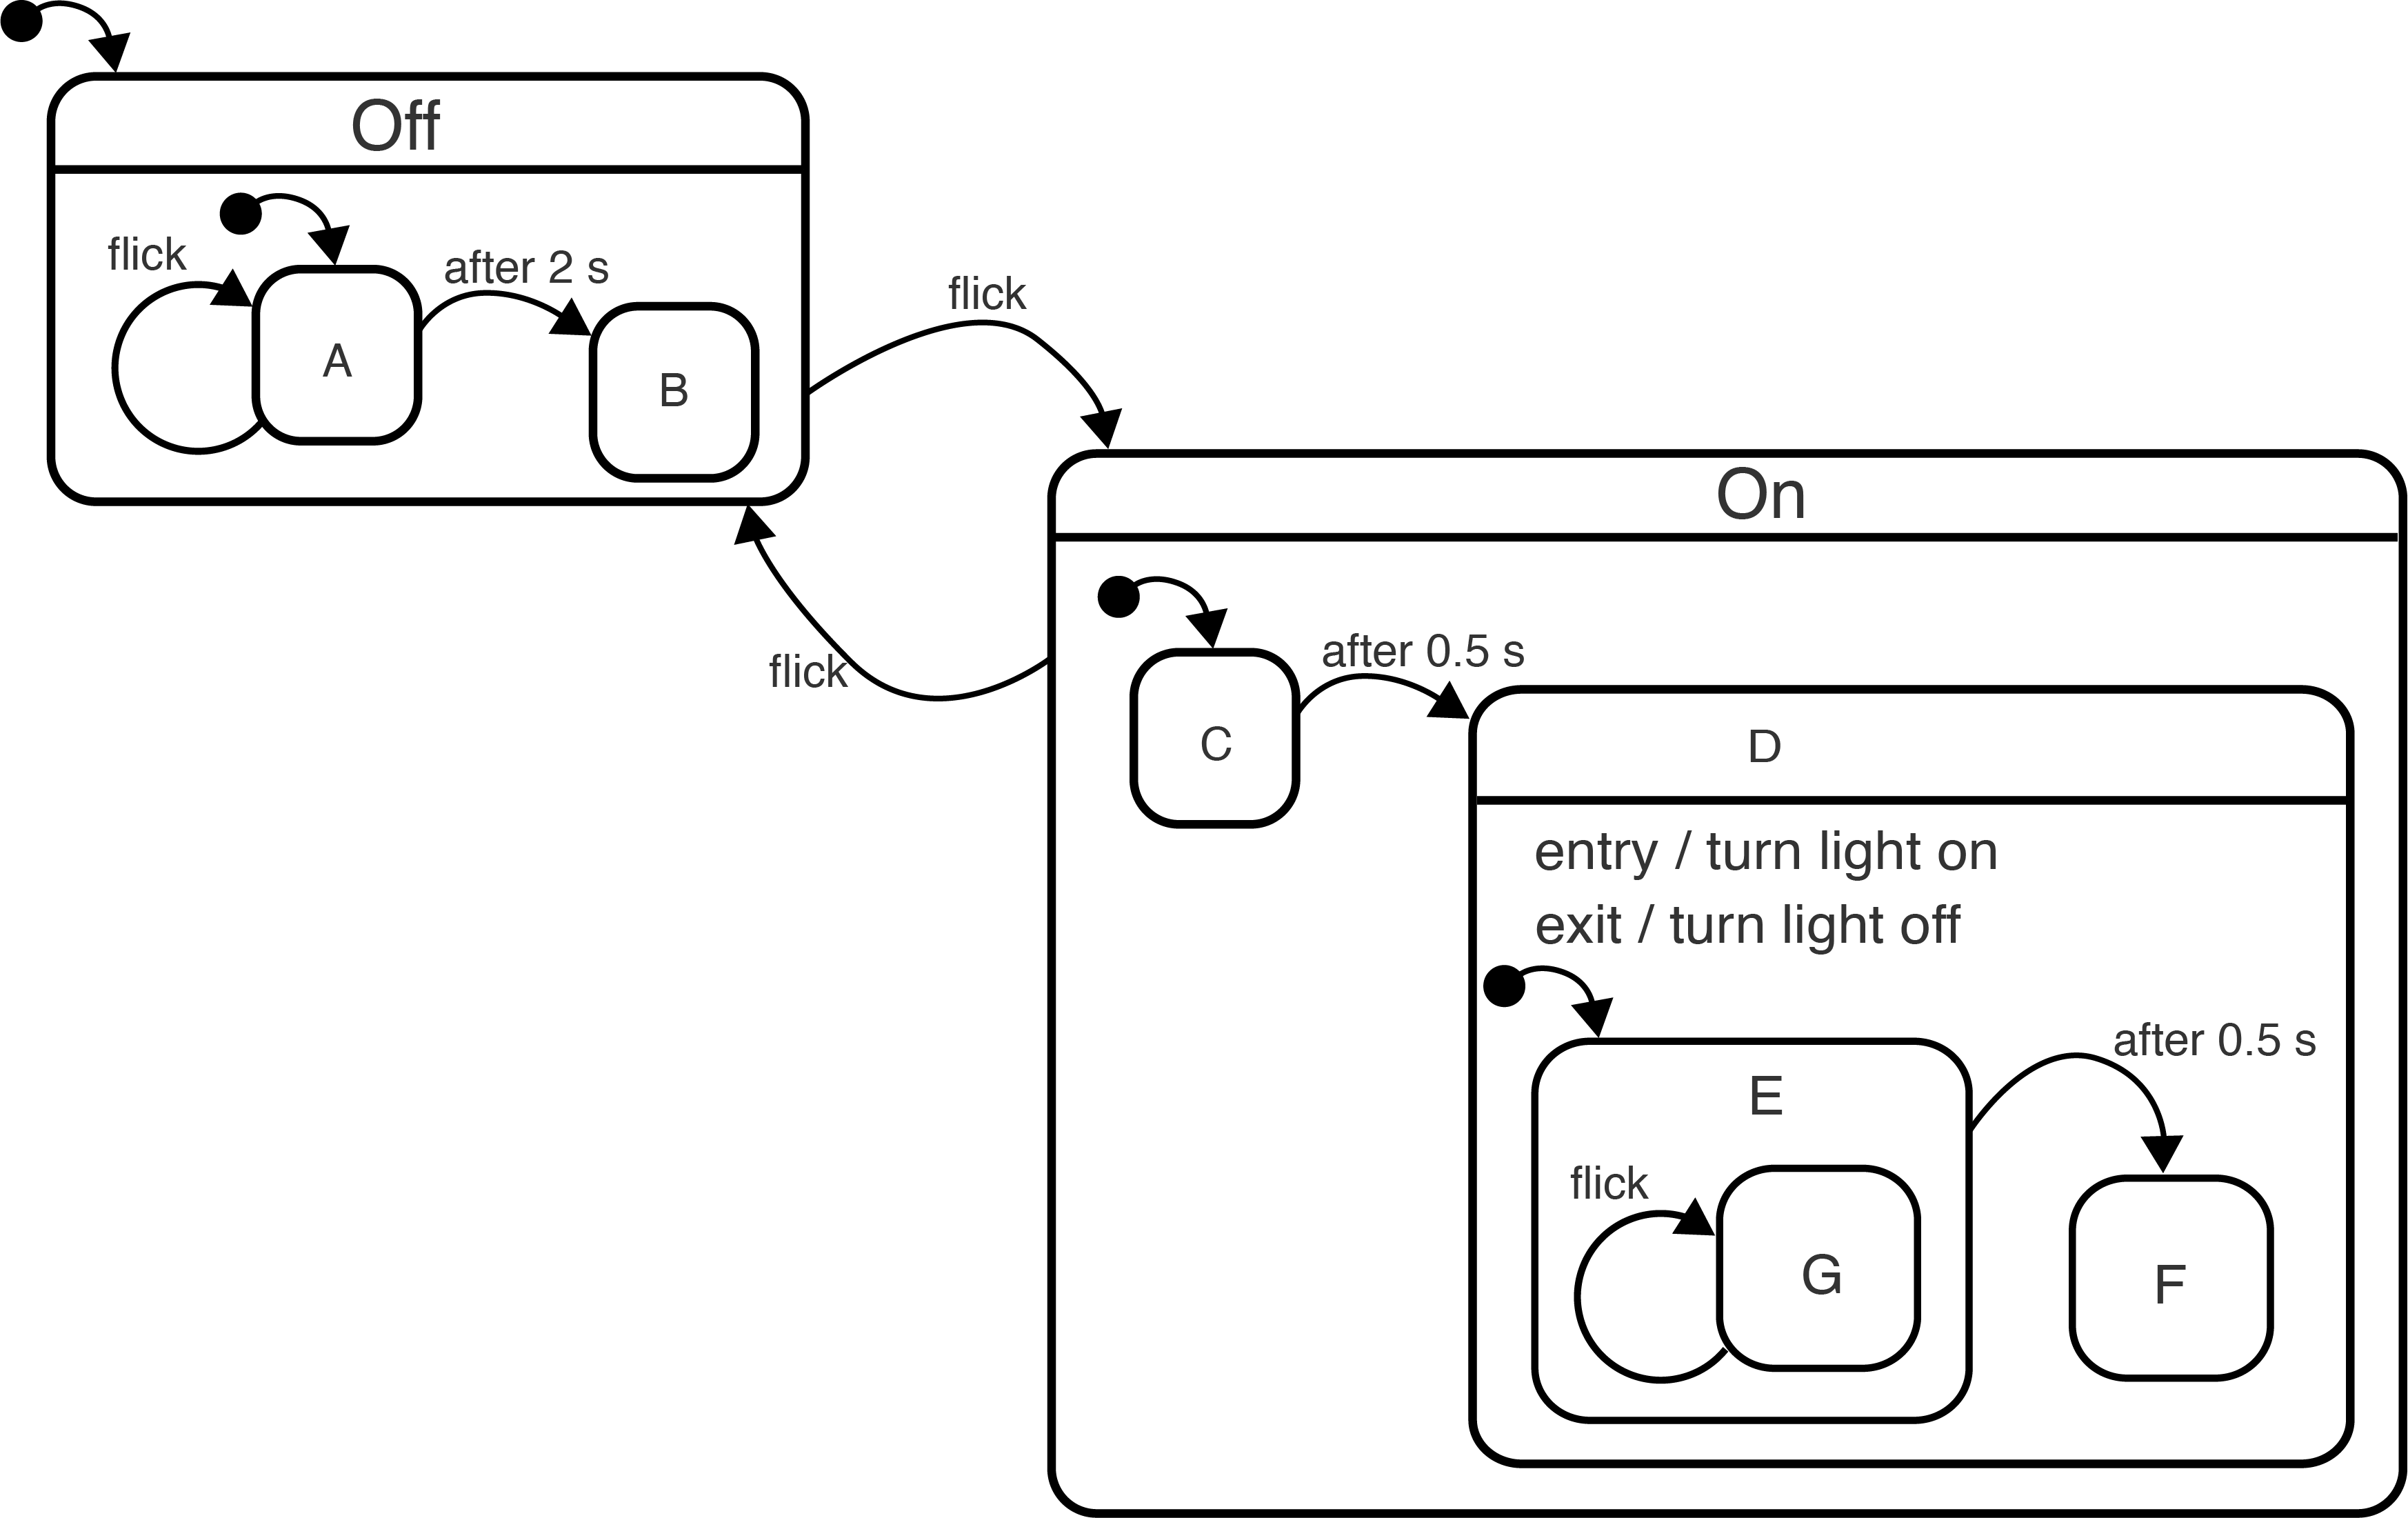
\includegraphics[width=\linewidth]{./images/on-off-delayed-exit-1.png}
\label{fig:statechart}
\caption{``When you flick a lightswitch, wait 0.5 seconds before turning
the light on, then once it's on wait 0.5 seconds before being able to
turn it back off again. When you flick it off, wait 2 seconds before you
can turn it on again.}
\end{figure}

They have an extensive set of documents that defend the consistency and
readability of statecharts on their
\href{https://statecharts.dev/}{homepage}, and my point here is not to
disagree with them. My point is instead that tools that aspire to the
status of generalized infrastructure can't ask people to dramatically
change the way they think about and do science. There are many possible
realizations of any given experiment, and each is more or less natural
to every person.

The problem here is really one of emphasis, BEADL seeks to solve
problems with inconsistencies in terminology by standardizing them, and
in order to do that seeks to standardize the syntax for specifying
experiments.

This means of standardization has many attractive qualities and is being
led by very capable researchers, but I think the project is illustrative
of how the differing structures of problems constrain the possible space
of tooling. Analysis tasks are often asynchronous, where the precise
timing of each node's completion is less important than the path
dependencies between different nodes. Analysis tasks often have a
clearly defined set of start, end, and intermediate cache points, rather
than branching or cyclical decision paths that change over multiple
timescales. Statecharts are a hierarchical abstraction of finite state
machines, the primary advantage of which is that they are better able to
incorporate continuous and history-dependent behavior, which cause state
explosion in traditional finite-state machines.

The difficulty of a controlled ontology for experimental frameworks is
perhaps better illustrated by considering a full experiment. In
Autopilot, a full experiment can be parameterized by the \texttt{.json}
files that define the task itself and the system-specific configuration
of the hardware. An
\href{https://gist.github.com/sneakers-the-rat/eebe675326a157df49f66f62c4e33a6e}{example
task} from our lab consists of 7 behavioral shaping stages of increasing
difficulty that introduce the animal to different features of a fairly
typical auditory categorization task. Each stage includes the parameters
for at most 12 different stimuli per stage, probabilities for presenting
lasers, bias correction, reinforcement, criteria for advancing to the
next stage, etc. So just for one relatively straightforward experiment,
in one lab, in one subdiscipline, there are \textbf{268 parameters} --
excluding all the default parameters encoded in the software.

How might we approach this problem differently, to accommodate diversity
of thought styles and to be complementary to our data and analysis
systems? The primary things we need from our experimental frameworks are
a) to be able to link a particular realization of an experiment with the
metadata that describes it, and b) to be able to produce similarly
metadata-rich data. Rather than linked data indicating code as in our
analysis frameworks, we might invert our strategy and think about code
that draws from linked data.

As an example, \href{https://docs.auto-pi-lot.com}{Autopilot} \citep{saundersAutopilotAutomatingBehavioral2019}  approaches the problem by
avoiding standardizing \emph{experiments} themselves, instead providing
smaller building blocks of experimental tools like hardware drivers,
data transformations, etc. and emphasizing understanding their use in
\emph{context.} This approach sacrifices some of the qualities of a
standardized system like being a logically complete or guaranteeing a
standardized vocabulary in order to better support integrating with
existing work patterns and making work cumulative. Because we can't
possibly predict the needs and limitations of a totalizing system, we
split the problem along a different set of concerns, those of the
elements of experimental practice, and give facility for describing how
they are used together.

For concrete example, we might imagine the lightswitch in an
autopilot-like framework like this:

\begin{Shaded}
\begin{Highlighting}[]
\ImportTok{from}\NormalTok{ autopilot.hardware.gpio }\ImportTok{import}\NormalTok{ Digital\_Out}
\ImportTok{from}\NormalTok{ time }\ImportTok{import}\NormalTok{ sleep}
\ImportTok{from}\NormalTok{ threading }\ImportTok{import}\NormalTok{ Lock}

\KeywordTok{class}\NormalTok{ Lightswitch(Digital\_Out):}
  \KeywordTok{def} \FunctionTok{\_\_init\_\_}\NormalTok{(}\VariableTok{self}\NormalTok{,}
\NormalTok{    off\_debounce: }\BuiltInTok{float} \OperatorTok{=} \DecValTok{2}\NormalTok{,}
\NormalTok{    on\_delay:     }\BuiltInTok{float} \OperatorTok{=} \FloatTok{0.5}\NormalTok{,}
\NormalTok{    on\_debounce:  }\BuiltInTok{float} \OperatorTok{=} \FloatTok{0.5}\NormalTok{):}
    \CommentTok{"""}
\CommentTok{    Args:}
\CommentTok{      off\_debounce (float): }
\CommentTok{        Time (s) before light can be turned back on}
\CommentTok{      on\_delay (float): }
\CommentTok{        Time (s) before light is turned on}
\CommentTok{      on\_debounce (float): }
\CommentTok{        Time (s) after turning on that light can\textquotesingle{}t be turned off}
\CommentTok{    """}
    \VariableTok{self}\NormalTok{.off\_debounce }\OperatorTok{=}\NormalTok{ off\_debounce}
    \VariableTok{self}\NormalTok{.on\_delay     }\OperatorTok{=}\NormalTok{ on\_delay}
    \VariableTok{self}\NormalTok{.on\_debounce  }\OperatorTok{=}\NormalTok{ on\_debounce}

    \VariableTok{self}\NormalTok{.on }\OperatorTok{=} \VariableTok{False}
    \VariableTok{self}\NormalTok{.lock }\OperatorTok{=}\NormalTok{ Lock()}

  \KeywordTok{def}\NormalTok{ switch(}\VariableTok{self}\NormalTok{):}
    \CommentTok{\# use a lock to make sure if}
    \CommentTok{\# called while waiting, we ignore it}
    \ControlFlowTok{if} \KeywordTok{not} \VariableTok{self}\NormalTok{.lock.acquire():}
      \ControlFlowTok{return}

    \CommentTok{\# if already on, switch off}
    \ControlFlowTok{if} \VariableTok{self}\NormalTok{.on: }
      \VariableTok{self}\NormalTok{.on }\OperatorTok{=} \VariableTok{False}
\NormalTok{      sleep(}\VariableTok{self}\NormalTok{.off\_debounce)}

    \CommentTok{\# otherwise switch on}
    \ControlFlowTok{else}\NormalTok{: }
\NormalTok{      sleep(}\VariableTok{self}\NormalTok{.on\_delay)}
      \VariableTok{self}\NormalTok{.on }\OperatorTok{=} \VariableTok{True}
\NormalTok{      sleep(}\VariableTok{self}\NormalTok{.on\_debounce)}

    \VariableTok{self}\NormalTok{.lock.release()}
\end{Highlighting}
\end{Shaded}

The class \texttt{Lightswitch} inherits from the \texttt{Digital\_Out}
class, which in turn inherits from \texttt{GPIO} and eventually
\texttt{Hardware}. This hierarchy of inheritance carries with it a
progressive refinement of meaning about what this class does. The terms
\texttt{off\_debounce}, \texttt{on\_delay}, and \texttt{on\_debounce}
are certainly not part of a controlled ontology, but the context of
their use bounds their meaning. Rather than being bound by, for example,
the abstract \texttt{Latency} term from
\href{https://scicrunch.org/scicrunch/interlex/view/ilx_0106040\#annotations}{interlex},
we have defined terms that we need to make a hardware object do what we
need it to. These terms don't have too much meaning on their own ---
there isn't even much in this class to uniquely identify it as a
``lightswitch'' beyond its name, it is just a timed digital output. What
makes them meaningful is how they are used.

The way Autopilot handles various parameters are part of set of layers
of abstraction that separate idiosyncratic logic from the generic form
of a particular \texttt{Task} or \texttt{Hardware} class. The general
structure of a two-alternative forced choice task is shared across a
number of experiments, but they may have different stimuli, different
hardware, and so on. Autopilot \texttt{Task}s use abstract references to
classes of hardware components that are required to run them, but
separates their implementation as a system-specific configuration so
that it's not necessary to have \emph{exactly the same} components
plugged into \emph{exactly the same} GPIO pins, etc. Task parameters
like stimuli, reward timings, etc. are similarly split into a separate
task parameterization that both allow \texttt{Task}s to be generic and
make provenance and experimental history easier to track. \texttt{Task}
classes can be subclasses to add or modify logic while being able to
reuse much of the structure and maintain the link between the root task
and its derivatives --- for example
\href{https://github.com/auto-pi-lot/autopilot-plugin-wehrlab/blob/9cfffcf5fe1886d25658d4f1f0c0ffe41c18e2cc/gap/nafc_gap.py\#L13-L49}{one
task we use} that starts a continuous background sound but otherwise is
the same as the root \texttt{Nafc} class. The result of these points of
abstraction is to allow exact experimental replication on inexactly
replicated experimental apparatuses.

This separation of the different components of an experiment is a
balance between reusable code and clear metadata: we might allow freedom
of terminology for each individual class, but by designing the system to
encourage reuse of flexible classes we reduce the number of times unique
terms need to be redefined. For example, we can imagine a trivial use of
our lightswitch inside a task measuring an experimental subject's
estimation of time intervals: we toggle the switch once some analog
sensor reaches a certain threshold, and then the subject tries to press
a button at the same time as the light turns on after a fixed delay.
While this is very similar to how Autopilot currently works, note that
we are using pseudocode to indicate how it might extend the system we're
describing.

\begin{Shaded}
\begin{Highlighting}[]
\ImportTok{from}\NormalTok{ autopilot }\ImportTok{import}\NormalTok{ Task}
\ImportTok{from}\NormalTok{ autopilot.data.modeling }\ImportTok{import}\NormalTok{ Field}
\ImportTok{from}\NormalTok{ datetime }\ImportTok{import}\NormalTok{ datetime, timedelta}

\KeywordTok{class}\NormalTok{ Controlled\_Switch(Task):}
  \CommentTok{"""}
\CommentTok{  A [[Discipline::Psychophysics]] experiment }
\CommentTok{  to measure [[Research Topic::Interval Estimation]].}
\CommentTok{  """}

  \KeywordTok{class}\NormalTok{ Params(Task.Param\_Spec):}
\NormalTok{    on\_delay: }\StringTok{\textquotesingle{}@si:seconds\textquotesingle{}} \OperatorTok{=}\NormalTok{ Field(}
\NormalTok{        description}\OperatorTok{=}\StringTok{"Delay (s) before turning light on"}\NormalTok{,}
\NormalTok{        parameterizes}\OperatorTok{=}\StringTok{"@jonny:hardware:Lightswitch"}\NormalTok{)}
\NormalTok{    threshold: }\BuiltInTok{float} \OperatorTok{=}\NormalTok{ Field(}
\NormalTok{        description}\OperatorTok{=}\StringTok{"Flick switch above this value"}\NormalTok{,}
\NormalTok{        is\_a}\OperatorTok{=}\StringTok{"@interlex:Threshold"}\NormalTok{)}

  \KeywordTok{class}\NormalTok{ TrialData(Task.TrialData\_Spec):}
\NormalTok{    switch\_time: datetime }\OperatorTok{=}\NormalTok{ Field(}
\NormalTok{        description}\OperatorTok{=}\StringTok{"Time the switch was flicked"}\NormalTok{)}
\NormalTok{    target\_time: datetime }\OperatorTok{=}\NormalTok{ Field(}
\NormalTok{        description}\OperatorTok{=}\StringTok{"Time the subject should respond"}\NormalTok{)}
\NormalTok{    response\_time: datetime }\OperatorTok{=}\NormalTok{ Field(}
\NormalTok{        description}\OperatorTok{=}\StringTok{"Time the subject did respond"}\NormalTok{)}
\NormalTok{    error: timedelta }\OperatorTok{=}\NormalTok{ Field(}
\NormalTok{        description}\OperatorTok{=}\StringTok{"Difference between target and response"}\NormalTok{,}
\NormalTok{        is\_a}\OperatorTok{=}\StringTok{"@psychophys:ReactionTime"}\NormalTok{)}


\NormalTok{  HARDWARE }\OperatorTok{=}\NormalTok{ \{}
    \StringTok{\textquotesingle{}sensor\textquotesingle{}}\NormalTok{: }\StringTok{\textquotesingle{}Analog\_In\textquotesingle{}}\NormalTok{,}
    \StringTok{\textquotesingle{}button\textquotesingle{}}\NormalTok{: }\StringTok{\textquotesingle{}Digital\_In\textquotesingle{}}\NormalTok{,}
    \StringTok{\textquotesingle{}lightswitch\textquotesingle{}}\NormalTok{: }\StringTok{\textquotesingle{}@jonny:hardware:Lightswitch\textquotesingle{}}
\NormalTok{  \}}

  \KeywordTok{def} \FunctionTok{\_\_init\_\_}\NormalTok{(}\VariableTok{self}\NormalTok{, }
\NormalTok{      on\_delay:}\BuiltInTok{float}\NormalTok{, }
\NormalTok{      threshold:}\BuiltInTok{float}\NormalTok{):}
    \VariableTok{self}\NormalTok{.on\_delay }\OperatorTok{=}\NormalTok{ on\_delay}
    \VariableTok{self}\NormalTok{.threshold }\OperatorTok{=}\NormalTok{ threshold}

    \BuiltInTok{super}\NormalTok{(Controlled\_Switch, }\VariableTok{self}\NormalTok{).}\FunctionTok{\_\_init\_\_}\NormalTok{()}
    \VariableTok{self}\NormalTok{.poll()}

  \KeywordTok{def}\NormalTok{ poll(}\VariableTok{self}\NormalTok{):}
    \ControlFlowTok{while} \VariableTok{self}\NormalTok{.running:}
      \ControlFlowTok{if} \VariableTok{self}\NormalTok{.hardware[}\StringTok{\textquotesingle{}sensor\textquotesingle{}}\NormalTok{].value }\OperatorTok{\textgreater{}} \VariableTok{self}\NormalTok{.threshold:}
        \VariableTok{self}\NormalTok{.hardware[}\StringTok{\textquotesingle{}lightswitch\textquotesingle{}}\NormalTok{].switch()}
\NormalTok{        switch\_time }\OperatorTok{=}\NormalTok{ datetime.now()}
\NormalTok{        target\_time }\OperatorTok{=}\NormalTok{ switch\_time }\OperatorTok{+} \VariableTok{self}\NormalTok{.on\_delay}

        \CommentTok{\# Wait for the subject to press the button}
\NormalTok{        response\_time }\OperatorTok{=} \VariableTok{self}\NormalTok{.hardware[}\StringTok{\textquotesingle{}button\textquotesingle{}}\NormalTok{].wait()}

        \CommentTok{\# Send the data for storage}
        \VariableTok{self}\NormalTok{.node.send(key}\OperatorTok{=}\StringTok{"DATA"}\NormalTok{, value}\OperatorTok{=}\NormalTok{\{}
            \StringTok{\textquotesingle{}switch\_time\textquotesingle{}}\NormalTok{: switch\_time,}
            \StringTok{\textquotesingle{}target\_time\textquotesingle{}}\NormalTok{: target\_time,}
            \StringTok{\textquotesingle{}response\_time\textquotesingle{}}\NormalTok{: response\_time,}
            \StringTok{\textquotesingle{}error\textquotesingle{}}\NormalTok{: target\_time }\OperatorTok{{-}}\NormalTok{ response\_time}
\NormalTok{          \})}
\end{Highlighting}
\end{Shaded}

In this example, we first define a data model (see section 3.2 - Data in
\citep{saundersAUTOPILOTAutomatingExperiments2022}) for the Tasks
\texttt{Params}, the data that the task produces as \texttt{TrialData},
and the \texttt{HARDWARE} that the task uses. Our \texttt{Params} each
have a \href{https://peps.python.org/pep-0483/}{type hint} indicating
what type of data they are, as well as a \texttt{Field} that gives
further detail about them. Specifically, we have exposed the
Lightswitch's \texttt{on\_delay} parameter, indicated that it will be in
seconds by referring to some namespace that defines SI units
\texttt{@si} and that it parameterizes the lightswitch object that we
defined above. The \texttt{TrialData} is similarly annotated, and by
default Autopilot will use this specification to create an hdf5 table to
store the values. The \texttt{HARDWARE} dictionary makes abstract
references the hardware objects that will be made available in the task,
each of which would have its configuration --- which GPIO pin they are
plugged into, the polarity of the signal, etc. --- using some local
system configuration. Finally, the single \texttt{poll()} method
continuously compares the value of the sensor to the threshold, switches
the lightswitch when the threshold is crossed, records the time the
button was pressed, and sends it for storage with its network node.

As before, we are using our experimental framework as an interface to
our linked data system. Currently, Autopilot uses a
\href{https://www.semantic-mediawiki.org/wiki/Semantic_MediaWiki}{semantic
wiki} to organize technical knowledge and to share
\href{https://docs.auto-pi-lot.com/en/latest/guide/plugins.html}{plugins}
- \url{https://wiki.auto-pi-lot.com}. In this case, I would write my
task and hardware classes inside a git repository and then add them to
Autopilot's
\href{https://wiki.auto-pi-lot.com/index.php/Autopilot_Plugins}{plugin
registry}, which uses a
\href{https://wiki.auto-pi-lot.com/index.php/Form:Autopilot_Plugin}{form}
to fill in semantic properties and allows further annotation in free
text and semantic markup.

We could instead imagine being able to document the task in its
\href{https://peps.python.org/pep-0257/}{docstring}, including
describing the relevant subdiscipline, research topic, and any other
relevant metadata. Rather than manually entering it in the wiki, then,
we might export the triplet annotations directly from the class and make
them available from my \texttt{@jonny} namespace and mirroring that to
the wiki. Since the plugin specifies its dependencies using standard
Python tools, it would then be possible for other researchers to use its
task and hardware objects by referring to them as above.

In our pseudocode, the (abbreviated) exported metadata for this task
might look like this:

\begin{Shaded}
\begin{Highlighting}[]
\NormalTok{\textless{}\#tasks:Controlled\_Switch\textgreater{}}
\NormalTok{  a @autopilot:Task}

\NormalTok{  hasDescription}
\NormalTok{    "A Psychophysics experiment }
\NormalTok{    to measure Interval Estimation."}

\NormalTok{  Discipline "Psychophysics"}
\NormalTok{  Research\_Topic "Interval Estimation"}

\NormalTok{  Params}
\NormalTok{    on\_delay @si:seconds}
\NormalTok{      hasDescription "..."}
\NormalTok{      parameterizes @jonny:hardware:Lightswitch}
\NormalTok{    ...}

\NormalTok{  TrialData}
\NormalTok{    switch\_time @python:datetime}
\NormalTok{    ...}

\NormalTok{  usesHardware}
\NormalTok{    @autopilot:hardware:Analog\_In}
\NormalTok{      hasID "sensor"}
\NormalTok{    @autopilot:hardware:Digital\_In}
\NormalTok{      hasID "button"}
\NormalTok{    @jonny:hardware:Lightswitch}
\NormalTok{      hasID "lightswitch"}
\end{Highlighting}
\end{Shaded}

and we might combine it with metadata that describes our particular use
of it like this, where we combine that task with a series of other
\texttt{level}s that shape the behavior, make it more challenging, or
measure something else entirely:

\protect\hypertarget{myproject-experiment}{}{}

\begin{Shaded}
\begin{Highlighting}[]
\NormalTok{\textless{}\#projects:my{-}project\textgreater{}}
\NormalTok{  a @autopilot:protocol}
\NormalTok{  experimenter @jonny}
\NormalTok{  ...}

\NormalTok{  level @jonny:tasks:Controlled\_Switch}
\NormalTok{    on\_delay 2}
\NormalTok{    threshold 0.5}
\NormalTok{    graduation @autopilot:graduation:ntrials}
\NormalTok{      n\_trials 200}

\NormalTok{  level @jonny:tasks:Another\_Task}
\NormalTok{    ...}

\NormalTok{  hardwareConfig}
\NormalTok{    button @autopilot:hardware:Digital\_In}
\NormalTok{      gpioPin 17}
\NormalTok{      polarity 1}
\NormalTok{    sensor @autopilot:hardware:Analog\_In}
\NormalTok{      usesPart @apwiki:parts:\textless{}Part\_Number\textgreater{}}
\NormalTok{      ...}
\end{Highlighting}
\end{Shaded}

On the other side, our output data can be automatically exported to
NWB\sidenote{Recall that we're using NWB for the sake of concreteness,
  but this argument applies to any standardized data format.}. Our
experimental framework knows that data contained within a
\texttt{TrialData} model is a \texttt{@nwb:behavior:BehavioralEvents}
object, and can combine it with the metadata in our task docstring and
system configuration. If we needed more specific data export - say we
wanted to record the timeseries of the analog sensor - we could use the
same \texttt{is\_a} parameter to declare it as a
\texttt{@nwb:TimeSeries} and create an extension to store the metadata
about the sensor alongside it\sidenote{Though this is a description of
  something we could build towards, v0.5.0 (at the time of writing
  released as alpha) of Autopilot has a
  \href{https://docs.auto-pi-lot.com/en/latest/changelog/v0.5.0.html}{data
  modeling} framework that should make this possible in future versions.}.

So while our code is mildly annotated and uses a mixture of standard and
nonstandard terminology, we make use of the structure of the
experimental framework to generate rich provenance to understand our
data and task in context. It's worth pausing to consider what this means
for our infrastructural system as a whole

To start, we have a means of integrating our task with the knowledge
that precedes it in the hardware and system configuration that runs it.
In addition to documenting plugins, among others, the Autopilot wiki
also has schema for
\href{https://wiki.auto-pi-lot.com/index.php/Autopilot_Behavior_Box}{custom
built} and
\href{https://wiki.auto-pi-lot.com/index.php/Parts}{off-the-shelf}
hardware like
\href{https://wiki.auto-pi-lot.com/index.php/TT_Electronics_OPB901L55}{sensors}
and \href{https://wiki.auto-pi-lot.com/index.php/HiFiBerry_Amp2}{sound
cards}. These correspond to local hardware configuration entries that
link them to the hardware classes required to use them\sidenote{Not yet,
  but this is planned development for future versions.}. That link can
be used bidirectionally: metadata about the hardware used to perform an
experiment can be used in the experiment and be included with the
produced data data, but the data from experiments can also be used to
document the hardware. That means that usage data like calibrations and
part longevity can be automatically collected and contributed to the
wiki and then used to automatically configure hardware in future uses.
This makes using the experimental framework more powerful, but also
makes building a communal library of technical knowledge a normal part
of doing experiments. Though the wiki is a transitional medium towards
what we will discuss in the next section, since contributions are
tracked and versioned that allows a currently undervalued class of
knowledge work to be creditable.

This gives us a different model of designing and engineering experiments
than we typically follow. Rather than designing most of it from scratch
or decoding cryptic methods sections, researchers could start with a
question and basic class of experiment, browse through various
implementations based on different sets of tools, see which hardware
they and analogous experiments use, which is then linked to the code
needed to run it. From some basic information researchers would then be
most of the way to performing an experiment: clone the task, download
the necessary system configuration information to set up the hardware,
make incremental modifications to make the experiment match what they
had designed, all the while contributing and being credited for their
work.

Much of this is possible because of the way that Autopilot isolates
different components of an experiment: hardware is defined separately
from tasks, both are separate from their local configuration. In
addition to thinking about how to design tools for our infrastructural
system, we can also think of the way it might augment existing tools.
Another widely used and extremely capable tool, Bonsai \citep{lopesBonsaiEventbasedFramework2015a, lopesNewOpenSourceTools2021}, is
based on XML documents that
\href{https://github.com/bonsai-rx/bonsai-examples/blob/cbc2c1decc11e1dc1df920421ef88a16fd2e184c/RoiTrigger/RoiTrigger.bonsai}{combine
the pattern of nodes} that constitute an experiment with specific
parameters like a
\href{https://github.com/bonsai-rx/bonsai-examples/blob/cbc2c1decc11e1dc1df920421ef88a16fd2e184c/RoiTrigger/RoiTrigger.bonsai\#L76-L85}{crop
bounding box}. That makes sharing and reusing tasks difficult without
exactly matching the original hardware configuration, but we could use
our metadata system to \emph{generate} code for Bonsai in addition to
consuming data from it. Given some schematic pattern of nodes that
describes the operation of the experiment, we could combine that with
the same notion of separable parameterization and hardware
configurations as we might use in Autopilot to generate the XML for a
bonsai workflow. As with analytical tools, our infrastructural system
could be used to make a wide array of experimental tools interoperable
with an evolving set of vernacular metadata schema.

Together, our data, experimental, and analytical infrastructures would
dramatically reshape what is possible in science. What we've described
is a complete provenance chain that can be traced from analyzed results
back through to the code and hardware used to perform the experiment.
Trivially, this makes the elusive workflow where experimental data is
automatically scooped up and analyzed as soon as it is collected that is
typically a hard-won engineering battle within a single lab the normal
mode of using the system. Developing tools that give researchers control
over the mode of exported data renders the act of cleaning data
effectively obsolete. The role of our experimental tool is to be able to
make use of collected technical knowledge, but also to lower the
barriers to using the rest of the system by integrating it with normal
experimental practice.

The effects on collaboration and metascience are deeper though. Most
scientific communication describes collecting and analyzing a single
dataset. Making sense of many experiments is only possible qualitatively
as a review or quantitatively as meta-analysis. Even if we have a means
of linking many datasets and analysis pipelines as in the previous
section, the subtle details in how a particular experiment is performed
matter: things as small as milliseconds of variation in valve timings
through larger differences in training sequences or task design
powerfully influence the collected data. This makes comparing data from
even very similar experiments --- to say nothing of a class of results
from a range of different experiments --- a noisy and labor-intensive
statistical process, to the degree that it's possible at all. This
system extends the horizon of meta-analysis to the experiment itself and
turns experimental heterogeneity into a strength rather than a weakness.
Is some result a byproduct of some unreported parameter in the
experimental code? Is a result only visible when comparing across these
different conditions? Individual experiments only allow a relatively
limited set of interpretations and inferences to be drawn, but being
able to look across the variation in experimental design would allow
phenomena to be described in the full richness supported by available
observations.

This would also effectively dissolve the ``file drawer problem.'' \citep{sterlingPublicationDecisionsTheir1959, francoPublicationBiasSocial2014}  Though malice is not uncommon in
science, I think it's reasonably fair to assume that most researchers do
not withhold data given a null result in order to ``lie'' about an
effect, but because there is no reward for a potentially laborious
cleaning and publication process. Collecting data that is clean and
semantically annotated at the time of acquisition resolves the problem.
Even without the analysis or paper, being able to index across
experiments of a particular kind would make it possible to have a much
fairer look at a landscape distorded by the publication process and
prevent us from repeating the same experiments because no one has
bothered to publish the null. This would also open new avenues for
collaboration as we will explore in the next section.

To review:

We have described a system of three component modalities: \textbf{data,
analytical tools, and experimental tools} connected by a \textbf{linked
data} layer. We started by describing the need for a
\textbf{peer-to-peer} data system that makes use of \textbf{data
standards} as an onramp to linked metadata. To interact with the system,
we described an identity-based linked data system that lets individual
people declare linked data resources and properties that link to
\textbf{content addressed} resources in the p2p system, as well as
\textbf{federate} into multiple larger organizations. We described the
requirements for \textbf{DAG-based analytical frameworks} that allow
people to declare individual nodes for a processing chain linked to
code, combine them into workflows, and apply them to data. Finally, we
described a design strategy for \textbf{component-based experimental
frameworks} that lets people specify experimental metadata, tools, and
output data.

This system as described is a two-layer system, with a few different
domains linked by a flexible metadata linking layer. The metadata system
as described is not merely \emph{inert} metadata, but metadata linked to
code that can \emph{do something} --- eg. specify access permissions,
translate between data formats, execute analysis workflows, parameterize
experiments, etc. Put another way, we have been attempting to describe a
system that \emph{embeds the act of sharing and curation in the practice
of science.} Rather than a thankless post-hoc process, the system
attempts to provide a means for aligning the daily work of scientists so
that it can be cumulative and collaborative. To do this, we have tried
to avoid rigid specifications of system structure, and instead described
a system that allows researchers to pluralistically define the structure
themselves.

\hypertarget{shared-knowledge}{%
\section{Shared Knowledge}\label{shared-knowledge}}

\begin{leftbar}
The Web is more a social creation than a technical one. I designed it for a social effect --- to help people work together --- and not as a technical toy. [...] We clump into families, associations, and companies. We develop trust across the miles and distrust around the corner. What we believe, endorse, agree with, and depend on is representable and, increasingly, represented on the Web. We all have to ensure that the society we build with the Web is of the sort we intend.

Tim Berners-Lee (1999) \textit{Weaving the Web} \citep{berners-leeWeavingWebOriginal1999}
\end{leftbar}

The remaining set of problems implied by the infrastructural system
sketched so far are the \emph{communication} and \emph{organization}
systems that make up the interfaces to maintain and use it. We can
finally return to some of the breadcrumbs laid before: the need for
negotiating over distributed and conflicting data schema, for
incentivizing and organizing collective labor, and for communicating
information within and without academia.

The communication systems that are needed double as \emph{knowledge
organization} systems. Knowledge organization has the rosy hue of
something that might be uncontroversial and apolitical --- surely
everyone involved in scientific communication wants knowledge to be
organized, right? The reality of scientific practice might give a hint
at our naïveté. Despite being, in some sense, itself an effort to
organize knowledge, \emph{scientific results effectively have no system
of explicit organization.} There is no means of, say, ``finding all the
papers about a research question.''\sidenote{Also see Eve Marder's
  recent short and characteristically refreshing piece which in part
  discusses the problem of keeping up with scientific literature the
  context of maintaining the joy of discovery \citep{marderMaintainingJoyDiscovery2022}.} The problem is so fundamental
it seems natural: the usual methods of using search engines, asking
around on Twitter, and chasing citation trees are flex tape slapped over
the central absence of a system for formally relating our work as a
shared body of knowledge.

Information capitalism, in its terrifying splendor, here too pits
private profit against public good. Analogously to the necessary
functional limitations of SaaS platforms, artificially limiting
knowledge organization opens space for new products and profit
opportunities. In their 2020 shareholder report, RELX, the parent of
Elsevier, lists increasing the number of journals and papers as a
primary means of increasing revenue \citep{RELXAnnualReport2020}.
This represents a shift in their business model from subscriptions to
deals like open access, which according to RELX CEO Erik Nils Engström
``is where revenue is priced per article on a more explicit basis'' \citep{relx2020ResultsPresentation2021}.

In the next breath, they describe how ``in databases \& tools and
electronic reference, representing over a third of divisional\sidenote{RELX
  is a huge information conglomerate, and scientific publication is just
  one division.} revenue, we continued to drive good growth through
content development and enhanced machine learning {[}ML{]} and natural
language processing {[}NLP{]} based functionality.''

What ML and NLP systems are they referring to? The 2019 report is a bit
more revealing (emphases mine):

\begin{leftbar}
Elsevier looks to enhance quality by building on its premium brands and
\textbf{grow article volume} through \textbf{new journal launches,} the
expansion of open access journals and growth from emerging markets; and
add value to core platforms by implementing capabilities such as
\textbf{advanced recommendations on ScienceDirect and social
collaboration through reference manager and collaboration tool
Mendeley.}

\textbf{In every market, Elsevier is applying advanced ML and NLP
techniques} to help researchers, engineers and clinicians perform their
work better. For example, in research, ScienceDirect Topics, a free
layer of content that enhances the user experience, uses \textbf{ML and
NLP techniques to classify scientific content and organise it
thematically,} enabling users to get faster access to relevant results
and related scientific topics. The feature, launched in 2017, is proving
popular, generating 15\% of monthly unique visitors to ScienceDirect via
a topic page. \textbf{Elsevier also applies advanced ML techniques that
detect trending topics per domain,} helping researchers make more
informed decisions about their research. \textbf{Coupled with the
automated profiling and extraction of funding body information from
scientific articles,} this process supports the whole researcher
journey; from planning, to execution and funding. \citep{RELXAnnualReport2019} 
\end{leftbar}

Reading between the lines, it's clear that the difficulty of finding
research is a feature, not a bug of their system. Their explicit
business model is to increase the number of publications and sell
organization back to us with recommendation services. The recommendation
system might be free\sidenote{``free''}, but the business is to maintain
the self-reinforcing system of prestige where researchers compete for
placement in highly visible journals to stand out among a wash of
papers, in the process reifying the mythology \citep{brembsPrestigiousScienceJournals2018}  of the ``great journals.''
With semantic structure to locate papers, it becomes much more difficult
to sell high citation count as a product --- people can find what they
need, rather than needing to pay attention to a few high-profile
journals. Without it, which papers might a paper discovery system
created by a publisher recommend? The transition from a strictly
journal-based discovery system to a machine learning powered search and
feed model mirrors the strategic displacement of explicit organization
by search in the rest of the digital economy, and presents similar
opportunities for profit. Every algorithmically curated feed is an
opportunity to sell ad placement\sidenote{a strategy that the
  reprehensible digital marketing disciplines call ``native
  advertising'' \citep{dekeyzerProcessingNativeAdvertising2021, koutsopoulosNativeAdvertisementSelection2016} } --- which they
proudly describe as looking very similar to their research content \citep{springernatureBrandedContent, elsevier360AdvertisingSolutions}.

The extended universe of profitmaking from knowledge disorganization
gets more sinister: Elsevier sells multiple products to recommend
`trending' research areas likely to win grants, rank scientists, etc.,
algorithmically filling a need created by knowledge disorganization. The
branding varies by audience, but the products are the same. For
pharmaceutical companies
\href{https://www.elsevier.com/solutions/professional-services/drug-design-optimization\#opportunity}{``scientific
opportunity analysis''} promises custom reports that answer questions
like ``Which targets are currently being studied?'' ``Which experts are
not collaborating with a competitor?'' and ``How much funding is
dedicated to a particular area of research, and how much progress has
been made?'' \citep{elsevierDrugDesignOptimization}. For
academics,
\href{https://www.elsevier.com/solutions/scival/features/topic-prominence-in-science\#how}{``Topic
Prominence in Science''} offers university administrators tools to
``enrich strategic research planning with portfolio overviews of their
own and peer institutions.'' Researchers get tools to ``identify experts
and potential cross-sector collaborators in specific Topics to
strengthen their project teams and funding bids and identify Topics
which are likely to be well funded.'' \citep{elsevierTopicProminenceScienceb}  This reflects RELX's transition
``from electronic reference, information reference tools, databases to
{[}\ldots{]} analytics and decision tools.'' \citep{relx2020ResultsPresentation2021}  Publishing is old news, the real money is
in tools for extending control through the rest of the process of
research.

These tools are, of course, designed for a race to the bottom --- if my
colleague is getting an algorithmic leg up, how can I afford not to?
Naturally only those labs that \emph{can} afford them and the costs of
rapidly pivoting research topics will benefit from them, making yet
another mechanism that reentrenches scientific inequity for profit.
Knowledge disorganization, coupled with a little surveillance capitalism
that monitors the activity of colleagues and rivals \citep{brembsReplacingAcademicJournals2021, hansonUserTrackingAcademic2019},
has given publishers powerful control over the course of science, and
they are more than happy to ride algorithmically amplified scientific
hype cycles in fragmented research bubbles all the way to the bank.

One more turn of the screw: the ability of the (former) publishers to
effectively invent the metrics that operationalize ``prestige'' in the
absence of knowledge organization systems gives them broad leverage with
governments and funding agencies. In an environment of continuously
dwindling budgets and legislative scrutiny, seemingly mutually
beneficial platform contracts offer the sort of glossy comfort that only
predictive analytics can. In 2020 the National Research Foundation of
Korea (NRF) and Elsevier published a joint report that used a
measurement derived from citation counts - ``Field-weighted citation
impact'', or FWCI - to argue for the underrated research prestige of
South Korea \citep{researchfoundationofkoreaSouthKoreaTechnological2020}. While I don't
dispute the value of South Korea's research program, the apparent
bargain that was struck is chilling. South Korea gets a very fancy
report arguing that more scientists in other countries should work with
theirs, and Elsevier gets to cement itself into the basic operation of
science. Elsevier controls the journals that can guarantee high citation
counts \emph{and} the metrics built on top of them. The Brain Korea
program Phase II report \sidenote{the result of another corporate
  collaboration with the Rand corporation.} \citep{seongBrainKorea212008}, issued just before the 2009 formation of the
NRF argued that rankings and funding should be dependent on citation
counts. The NRF now relies on SciVal and their FWCI measurement as a
primary means of ranking researchers and determining funding, built into
the Brain Korea 21 funding system \citep{elsevierCaseStudyNational2019, elsevierkoreaSciValHwalyongeulWihan2021}. Without exaggeration, scientific disorganization and reliance on
citation counts allowed Elsevier to buy control over the course of
research in South Korea.

The consequences for science are hard to overstate. In addition to
literature search being an unnecessarily huge sink of time and labor,
science operates as a wash of tail-chasing results that only rarely seem
to cumulatively build on one another. The need to constantly reinforce
the norm that purposeful failure to cite prior work is research
misconduct is itself a symptom of how engaging with a larger body of
work is both extremely labor intensive and \emph{strictly optional} in
the communication regime of journal publication. The combination of more
publications translating into more profit and the strategic
disorganization of science contributes to conditions for scientific
fraud. An entirely fraudulent paper can be undetectable even by domain
experts. Since papers can effectively be islands --- given legitimacy by
placement in a journal strongly incentivized to accept all comers ---
and there is no good means of evaluating them in context with their
immediate semantic neighbors, investigating fraud is extremely time
consuming and almost entirely without reward. And since traditional peer
review happens once, rather than as a continual public process, the only
recourse outside of posting on PubPeer is to wait on journal editorial
boards to self-police by reviewing each individual complaint. Forensic
peer-reviewers have been ringing the alarm bell, saying that there is
``no net'' to bad research \citep{heathersRealScandalIvermectin2021}, and brave and highly-skilled investigators like
\href{https://scienceintegritydigest.com/}{Elisabeth Bik} have found
thousands of papers with evidence of purposeful manipulation \citep{shenMeetThisSuperspotter2020, bikPrevalenceInappropriateImage2016}.
The economic structure of for-profit journals pits their profit model
against their function as providing a venue for peer review --- the one
function most scientists are still sympathetic to. Trust in science is
critical for addressing our most dire problems from global pandemics to
climate change \citep{westMisinformationScience2021}, but
attitudes towards scientists are lukewarm at best \citep{kennedyAmericansTrustScientists2022}. Even when it isn't fake news,
why would anyone trust us when it's \emph{effectively impossible} to
find or assess the quality of scientific information? \citep{krauseTrustFallacyScientists2021}  Not even scientists can: despite
the profusion of papers, by some measures progress in science has slowed
to a crawl \citep{chuSlowedCanonicalProgress2021}.

While Chu and Evans \citep{chuSlowedCanonicalProgress2021} 
correctly diagnose \emph{symptoms} of knowledge disorganization like the
need to ``resort to heuristics to make continued sense of the field''
and reliance on canonical papers, by treating the journal model as a
natural phenomenon and citation as the only means of ordering research,
they misattribute root \emph{causes.} The problem is not people
publishing \emph{too many papers,} or a \emph{breakdown of traditional
publication hierarchies,} but the \emph{staggering profitability of
knowledge disorganization.} Knowledge disorganization is precisely the
precondition of information-as-capital and the outcome of its
concentration by our century's robber barons (see \citep{ellenwoodInformationHasValue2020}). Their prescription for ``a
clearer hierarchy of journals'' misses the role of organizing scientific
work in journals ranked by prestige, rather than by the content of the
work, as a potentially major driver of extremely skewed citation
distributions. It also misses the publisher's stated goals of
\emph{publishing more papers} within an ecosystem of algorithmic
recommendations, and there is nothing recommendation algorithms love
recommending more than things that are already popular. Without
diagnosing knowledge disorganization as a core part of the business
model of scientific publishers, we can be led to prescriptions that
would make the problem worse.

It's hard to imagine an alternative to journals that doesn't look like,
well, journals. While a full treatment of the journal system is outside
the scope of this paper, the system we describe here renders them
\emph{effectively irrelevant} by making papers as we know them
\emph{unnecessary.} Rather than facing the massive collective action
problem of asking everyone to change their publication practices on a
dime, by reconsidering the way we organize the surrounding
infrastructure of science we can flank journals and replace them ``from
below'' with something qualitatively more useful.

Beyond journals, the other technologies of communication that have been
adopted out of need, though not necessarily design, serve as
\href{https://en.wikipedia.org/wiki/Desire_path}{desire paths} that
trace other needs for scientific communication. As a rough sample:
Researchers often prepare their manuscripts using platforms like Google
Drive, indicating a need for collaborative tools in preparation of an
idea. When working in teams, we often use tools like Slack to plan our
work. Scientific conferences reflect the need for federated
communication within subdisciplines, and we have adopted Twitter as a de
facto platform for socializing and sharing our work to a broader
audience. We use a handful of blogs and other sites like
\href{https://edspace.american.edu/openbehavior/}{OpenBehavior} \citep{whiteFutureOpenOpenSource2019},
\href{https://open-neuroscience.com/}{Open Neuroscience}, and many
others to index technical knowledge and tools. Last but not finally, we
use sites like \href{https://pubpeer.com}{PubPeer} and ResearchGate for
comment and criticism.

These technologies point to a few overlapping and not altogether binary
axes of communication systems.

\begin{itemize}

\item
  \textbf{Durable vs Ephemeral} - journals seek to represent information
  as permanent, archival-grade material, but scientific communication
  also necessarily exists as contextual, temporally specific snapshots.
\item
  \textbf{Structured vs Chronological} - scientific communication both
  needs to present itself as a structured basis of information with
  formal semantic linking, but also needs the chronological structure
  that ties ideas to their context. This axis is a gradient from
  formally structured references, through intermediate systems like
  forums with hierarchical topic structure that embeds a feed, to the
  purely chronological feed-based social media systems.
\item
  \textbf{Messaging vs Publishing} - Communication can be
  person-to-person, person-to-group with defined senders and recipients,
  or person-to-all statement to an undefined public. This ranges from
  private DMs through domain-specific tool indexes like OpenBehavior
  through the uniform indexing of Wikipedia.
\item
  \textbf{Public vs.~Private} - Who gets to read, who gets to
  contribute? Communication can be composed of entirely private notes to
  self, through communication in a lab, collaboration group, discipline,
  and landing in the entirely public realm of global communication.
\item
  \textbf{Formal vs.~Informal} - Journal articles and encyclopedia-bound
  writing that conforms to a particular modality of expression vs.~a
  vernacular style intended to communicate with people outside the
  jargon culture.
\item
  \textbf{Push vs.~Pull} - Do you go to get information from a reference
  location, or does information come to you as an alert or message? Or,
  generally, where is the information ``located,'' is an annotation
  pushed and overlaid on a document, or stored elsewhere requiring the
  audience to explicitly pull it?
\end{itemize}

``Peer reviewed vs.~unrefereed'' is purposely excluded as an axis of
communication tools, as the ability to review and annotate multiple
versions of a document --- subject to the context of the medium ---
should be a basic part of any communication system. Fear over losing the
at once immutable but also paradoxically fragile ecosystem of
journal-led peer review is one of the first strawmen that stops
consideration of radically reorganizing scientific
communication\sidenote{For a recent example, see the responses to Dan
  Goodman's argument why he has stopped doing pre-publication peer
  review altogether \citep{goodmanCurrentSystemJournals2022, goodmanEndingSupportLegacy2022 } }. The belief that peer review as
we know it is an intrinsic part of science is ahistorical (eg. \citep{baldwinScientificAutonomyPublic2018}), and the belief that
journal-led peer review is somehow a unique venue for evaluating
scientific work ignores the immense quantity of criticism and discussion
that happens in almost every communicative context, scientific and
otherwise. The notion that the body of scientific knowledge is best
curated by passing each paper through a gauntlet of three anonymous
reviewers, after which it becomes Fact is ridiculous on its face.
Focusing on preserving peer review is a red herring that unnecessarily
constrains the possible forms of scientific communication. Instead we
will try and sketch systems that address the needs for communication and
knowledge organization left unmet precisely because of the primacy of
peer reviewed journal publications.

Clearly a variety of different types of communication tools are needed,
but there is no reason that each of them should be isolated and
inoperable with the others. We have already seen several of the ideas
that help bring an alternative into focus. Piracy communities
demonstrate ways to build social systems that can sustain distributed
infrastructure. Federated and protocol-based systems show us that we
don't need to choose between a single monolithic system or many
disconnected ones, but can have a heterogeneous space of tools linked by
a basic protocol. The semantic web gives us the unfilled promise of
triplet links as a very general means of structuring data and building
interfaces for disparate systems. We can bridge these lessons with some
from wiki culture to get a more practical sense of distributed
governance and organization. Together with our sketches of data,
analytical, and experimental tools we can start imagining a system for
coordinating them --- as well as displacing some of the more intractable
systems that misstructure the practice of science.

\hypertarget{the-wiki-way}{%
\subsection{The Wiki Way}\label{the-wiki-way}}

\begin{leftbar}
If we take radical collaboration as our core, then it becomes clear that
extending Wikipedia's success doesn't simply mean installing more copies
of wiki software for different tasks. It means figuring out the key
principles that make radical collaboration work. What kinds of projects
is it good for? How do you get them started? How do you keep them
growing? What rules do you put in place? What software do you use? \citep{swartzMakingMoreWikipedias2006} 
\end{leftbar}

\begin{leftbar}
So that's it --- insecure but reliable, indiscriminate and subtle, user
hostile yet easy to use, slow but up to date, and full of difficult,
nit-picking people who exhibit a remarkable community camaraderie.
Confused? Any other online community would count each of these
``negatives'' as a terrible flaw, and the contradictions as impossible
to reconcile. Perhaps wiki works because the other online communities
don't. \citep{leufWikiWayQuick2001a}  and in
\href{http://wiki.c2.com/?WhyWikiWorks}{WhyWikiWorks}\end{leftbar} \sidenote[][-3.2cm]{Interestingly, this quote is almost, but not exactly the same as that on \href{http://wiki.c2.com/?WhyWikiWorks}{Ward's wiki}: "So that's it - insecure, indiscriminate, user-hostile, slow, full of difficult, nit-picking people, and frivolous. Any other online community would count each of these strengths as a terrible flaw. Perhaps wiki works because the other online communities do not." I can't tell if Ward Cunningham wrote the original entry in the wiki, but in any case seems to have found a bit of optimism in the book.}


Aside from maybe the internet itself, there is no larger public digital
knowledge organization effort than Wikipedia. While there are many
lessons to be learned from Wikipedia itself, it emerged from a prior
base of thought and experimentation in radically permissive,
self-structuring read/write --- sometimes called ``peer production''
\citep{hillWikipediaEndOpen2019}  --- communities. Wikis are now
quasi-ubiquitous\sidenote{though their corporate manifestations would
  probably be unrecognizable to the project early wiki users imagined.},
perhaps largely thanks to Wikipedia, but its specific history and intent
to be an \emph{encyclopedia} entwines it with a very particular
technological and social system that obscures some of the broader dreams
of early wikis.

Aaron Swartz recounts a quote from Jimmy Wales, co-founder of Wikipedia:

\begin{leftbar}
``I'm not a wiki person who happened to go into encyclopedias,'' Wales
told the crowd at Oxford. ``I'm an encyclopedia person who happened to
use a wiki.'' \citep{swartzWhoWritesWikipedia2006} 
\end{leftbar}

And further describes how this origin and mission differentiates it from
other internet communities:

\begin{leftbar}
But Wikipedia isn't even a typical community. Usually Internet
communities are groups of people who come together to discuss something,
like cryptography or the writing of a technical specification. Perhaps
they meet in an IRC channel, a web forum, a newsgroup, or on a mailing
list, but the focus is always something ``out there'', something outside
the discussion itself.

But \textbf{with Wikipedia, the goal is building Wikipedia.} It's not a
community set up to make some other thing, it's a community set up to
make itself. And since Wikipedia was one of the first sites to do it, we
know hardly anything about building communities like that. \citep{swartzMakingMoreWikipedias2006} 
\end{leftbar}

We know a lot more now than in 2006, of course, but Wikipedia still has
outsized structuring influence on our beliefs about what Wikis can be.
Wikipedia has since spawned a
\href{https://meta.wikimedia.org/wiki/Complete_list_of_Wikimedia_projects}{large
number} of technologies and projects like
\href{https://meta.wikimedia.org/wiki/Wikidata}{Wikidata} and
\href{https://commons.wikimedia.org/wiki/Main_Page}{Wikimedia Commons},
each with their own long and occasionally torrid histories. I won't
dwell on the obvious and massive feat of collective organization that the
greater Wikipedia project represents --- we should build on and
interoperate with its projects and respect the amount of work the
foundation and its editors have put in to preserve free access to
information, but learning from its imperfections is more useful to us
here, especially for things that aren't encyclopedias. The dream of a
centralized, but mass-edited ``encyclopedia of everything'' seems to be
waning, and its slow retreat from wild openness has run parallel to a
long decline in contributors \citep{hillWikipediaEndOpen2019, halfakerRiseDeclineOpen2013}. Throughout that time, there has been a
separate (and largely skeptical) set of wiki communities holding court
on what a radically open web can be like, inventing their worlds in real
time. These communities have histories that are continuous with one
another, and in their mutual reaction and inspiration sometimes teach
similar lessons from across the divides of their very different
structure.

The first wiki was launched in 1995\sidenote{it's complicated:
  \href{http://wiki.c2.com/?WardsWikiTenthAnniversary}{WardsWikiTenthAnniversary}}
(\href{http://wiki.c2.com/}{it's still up}) and came to be known as
Ward's wiki after its author
\href{http://wiki.c2.com/?WardCunningham}{WardCunningham}. Technically,
it was extremely simple: a handful of
\href{http://wiki.c2.com/?TextFormattingRules}{TextFormattingRules} and
use of \href{http://wiki.c2.com/?WikiCase}{WikiCase} where if you
\href{http://wiki.c2.com/?JoinCapitalizedWords}{JoinCapitalizedWords}
you create a link to a (potentially new)
\href{http://wiki.c2.com/?WikiPage}{WikiPage} --- and the ability for
anyone to edit any page. These very simple
\href{http://wiki.c2.com/?WikiDesignPrinciples}{WikiDesignPrinciples}
led to a sprawling and continuous conversation that spanned more than a
\href{http://wiki.c2.com/?WardsWikiTenthAnniversary}{decade} and
thousands\sidenote{\href{http://c2.com/wiki/history/}{23,244} unique
  page names according to the edit history, but the edit history was
  also purposely pruned from time to time.} of pages that, because of
the nature of the medium, is left fully preserved in amber. Those
conversations are a history of thought on what makes wiki communities
work (eg. \href{http://wiki.c2.com/?WhyWikiWorks}{WhyWikiWorks},
\href{http://wiki.c2.com/?WhyWikiWorksNot}{WhyWikiWorksNot}), and what
is needed to sustain them.

One tension that emerged early without satisfying resolution is the
balance between
``\href{http://wiki.c2.com/?DocumentMode}{DocumentMode}'' writing that
serves as linearly-readable reference material, similar to that of
Wikipedia, and ``\href{http://wiki.c2.com/?ThreadMode}{ThreadMode}''
writing that is a nonlinear representation of a conversation. Order vs
spontaneity is a fundamental challenge of inventing culture in
plaintext. The purpose of using a wiki as opposed to other technologies
that existed at the time like bulletin boards, newsgroups, IRC, etc. was
that it provided a means of fluid structure\sidenote{Giving a means of
  organizing the writing of the Portland Pattern Repository was the
  reason for creating Ward's Wiki in the first place.}. The parallel
need to communicate and attribute work made it a seeming inevitability
that even if you went out of your way to restructure a lot of writing
into a sensible DocumentMode page, someone would soon after create a new
horizontal divider and start a fresh ThreadMode section.

Ward Cunningham and other more organizationally-oriented contributors
opposed ThreadMode (eg.
\href{http://wiki.c2.com/?ThreadModeConsideredHarmful}{ThreadModeConsideredHarmful},
\href{http://wiki.c2.com/?InFavorOfDissertation}{InFavorOfDissertation})
for a number of reasons, largely due to the
\href{http://wiki.c2.com/?ThreadMess}{ThreadMess} and
\href{http://wiki.c2.com/?WikiChaos}{WikiChaos} it had the potential of
creating.

\begin{leftbar}
I occasionally suggest how this site should be used. My
\href{http://wiki.c2.com/?GoodStyle}{GoodStyle} suggestions have been
here since the beginning and are linked from the edit page should anyone
forget. I have done my best to discourage dialog
\href{http://wiki.c2.com/?InFavorOfDissertation}{InFavorOfDissertation}
which offers a better fit to this medium. I've been overruled. I will
continue to make small edits to pages for the sake of brevity. --
\href{http://wiki.c2.com/?WardCunningham}{WardCunningham} \citep{C2wikiWikiHistory} 
\end{leftbar}

Most pages are thus a combination of both, usually with some
DocumentMode text at the top with ThreadMode conversations interspersed
throughout without necessarily having any clean delineation between the
two. Far from just being raw disorder, this mixed mode of writing gave
it a peculiar character of being \emph{both} a folk reference for a
library of concepts \emph{as well as} a history of discussion that made
the contingency of that reference material plain. Beka Valentine put it
well:

\begin{leftbar}
c2wiki is an exercise in dialogical methods. of laying bare the fact
that knowledge and ideas are not some truth delivered from On High, but
rather a social process, a conversation, a dialectic, between various
views and interests \citep{valentineC2wikiExerciseDialogical2021} 
\end{leftbar}

This tension and its surrounding discussions point to the need for
multiple representations of a single idea: that both the social and
reference representations of a concept are valuable, but aren't
necessarily best served by being represented in the same place. There
was relatively common understanding that the intended order of things
was to have many ThreadMode conversations that would gradually be
converted to DocumentMode in a process of
\href{http://wiki.c2.com/?BrainStormFirstCleanLater}{BrainStormFirstCleanLater}.
Many \href{http://wiki.c2.com/?ConvertThreadModeToDocumentMode}{proposed
solutions} orbit around making parallel pages with similar names (like
\textless pagename\textgreater Discussion) to clean up a document while
preserving the threads (though there were plenty of interesting
alternatives, eg.
\href{http://wiki.c2.com/?DialecticMode}{DialecticMode})\sidenote{Contemporary
  wikis have continued this conversation, see
  \href{https://communitywiki.org/wiki/DocumentsVsMessages}{DocumentsVsMessages}
  on communitywiki.org}.

Wikipedia, in its attendant
\href{http://wiki.c2.com/?WikiEngines}{WikiEngine}
\href{https://meta.wikimedia.org/wiki/MediaWiki}{MediaWiki}, cut the
Gordian Knot by splitting each page into a separate \emph{Article} and
\emph{Talk} pages, with the talk page in its own \textbf{Namespace} --
eg. \href{https://en.wikipedia.org/wiki/Gordian_Knot}{Gordian\_Knot} vs
\href{https://en.wikipedia.org/wiki/Talk:Gordian_Knot}{Talk:Gordian\_Knot}.
Talk pages resemble a lot of the energy of early wikis: disorganized,
sometimes silly, sometimes angry, and usually charmingly pedantic.
Namespaces extend the traditional ``everything is a page'' notion
encoded in the WikiCase link system by giving different pages different
roles. In addition to having parallel conversations on articles and talk
pages, it is possible to have template pages that can be included on
wiki pages with
\texttt{\{\{double\ curly\ bracket\}\}}
syntax -- eg.
\href{https://en.wikipedia.org/wiki/Template:Citation_needed}{Template:Citation\_Needed}
renders
\texttt{\{\{Citation\ needed\}\}} as
{[}citation needed{]}. Talk pages have their own \textbf{functional
differentiation,} with features for threading and annotating discussions
that aren't present on the main article pages (see
\href{https://en.wikipedia.org/wiki/Wikipedia:Flow}{Wikipedia:Flow} \citep{WikipediaFlow2021}). Generalized beyond the context of wikis,
functional differentiation of a single item into its multiple
representations is relatively common in computing: eg. this document
exists as a
\href{https://github.com/sneakers-the-rat/infrastructure}{git
repository}, the
\protect\hypertarget{gobackhere}{}{\href{https://jon-e.net/infrastructure/goback.html}{rendered
page}}, a
\href{https://jon-e.net/infrastructure/tex/decentralized_infrastructure_render.pdf}{pdf},
hypothes.is annotations, etc.

The complete segregation of discussion to Talk pages is driven by
Wikipedia's exclusivity as an encyclopedia, with reminders that it is
the
``\href{https://en.wikipedia.org/wiki/Wikipedia:Don't_lose_the_thread\#Move_to_the_article_talk_page}{sole
purpose}'' peppered throughout the rules and guidelines. The presence of
messy subjective discussions would of course be discordant with the very
austere and ``neutral'' articles of an encyclopedia. There are no
visible indications that the talk pages even exist in the main text, and
so even deeply controversial topics have no references to the
conversations in talk pages that contextualize them --- despite this
being a requested feature by both administrators and editors \citep{schneiderUnderstandingImprovingWikipedia2011}.

Talk pages serve as one of the primary points of coordination and
conflict resolution on Wikipedia, and also provide a low-barrier
entrypoint for questions posed to a space they perceive to be ``an
approachable community of experts'' \citep{viegasTalkYouType2007}.
The separation of Talk pages and the
\href{https://en.wikipedia.org/wiki/Wikipedia:Talk_page_guidelines}{labyrinthine
rules} governing their use function to obscure the dialogical and
collective production of knowledge at the heart of wikis and Wikipedia.
The body of thought that structures Wikipedia, most of which is in its
\href{https://en.wikipedia.org/wiki/Wikipedia:Community_portal}{Wikipedia:*}
namespace, is immense and extremely valuable, but is largely hidden
except from those who care to look for it. Since Wikipedia is ``always
already there'' often without trace of its massively collective nature,
relatively few people ever contribute to it. Reciprocally, since
acknowledging personal contribution is or point of view is
\href{https://en.wikipedia.org/wiki/Wikipedia:No_original_research}{explicitly}
against some of its
\href{https://en.wikipedia.org/wiki/Wikipedia:Neutral_point_of_view}{core}
policies and
\href{https://en.wikipedia.org/wiki/Wikipedia:Avoid_thread_mode}{traditions},
there is little public credit outside the Wikipedia community itself for
the labor of maintaining it.

The forking of Wards Wikis into the first
\href{http://wiki.c2.com/?SisterSites}{SisterSites} teaches a parallel
strain of lessons. Ward's Wiki started as a means of organizing
knowledge for the Portland Pattern Repository\sidenote{The initial
  motivations are actually stunningly close to the kinds of
  communication and knowledge organization problems we are still solving
  today (even in this piece) \\ "Cunningham had developed a
  database to collect the contributions of the listserv members. He had
  noticed that the content of the listserv tended to get buried, and
  therefore the most recent post might be under-informed about posts
  which came before it. The way around this problem was to collect ideas
  in a database, and then edit those ideas rather than begin anew with
  each listserv posting. Cunningham's post states that ``The plan is to
  have interested parties write web pages about the People, Projects and
  Patterns that have changed the way they program. Short stories that
  hint at patterns are welcome too.'' As to the rhetorical expectations,
  Cunningham added ``The writing style is casual, like email or netnews,
  but doesn't have to be so repetitive since the things being discussed
  don't disappear. Think of it as a moderated list where anyone can be
  moderator and everything is archived. It's not quite a chat, still,
  conversation is possible." - \citep{cummingsWhatWasWikiWhy2009} }, a programming community (referred to as
\href{http://wiki.c2.com/?DesignPatterns}{DesignPatterns} below), and in
1998 they were overwhelmed with proponents of
\href{http://wiki.c2.com/?ExtremeProgramming}{ExtremeProgramming} (or
XP), which caused the first fissure in the wiki:

\begin{quote}
XP advocates seemed to be talking about XP at every possible opportunity
and seemingly on every page with content the least bit related to
software development. This annoyed a number people who were here to
discuss patterns, leading to the tag
\href{http://wiki.c2.com/?XpFreeZone}{XpFreeZone}, as a request not to
talk about ExtremeProgramming on that page.

It was difficult to pick out the
\href{http://wiki.c2.com/?DesignPatterns}{DesignPatterns} discussion on
\href{http://wiki.c2.com/?RecentChanges}{RecentChanges}\sidenote{Recent
  Changes was the dominant, if not controversial means of keeping track
  with recent wiki traffic, see
  \href{http://wiki.c2.com/?RecentChangesJunkie}{RecentChangesJunkie}},
because most of the activity was related to ExtremeProgramming.
Eventually, most of the
\href{http://wiki.c2.com/?DesignPatterns}{DesignPatterns} people left,
to discuss patterns in a ``quieter'' environment, and people started
referring to this site as
\href{http://wiki.c2.com/?WardsWiki}{WardsWiki} instead of the
\href{http://wiki.c2.com/?PortlandPatternRepository}{PortlandPatternRepository}
\citep{C2wikiWikiHistory} 
\end{quote}

One of the first and most influential Sister Sites was
\href{http://meatballwiki.org/}{Meatball Wiki}, described on Wards Wiki:

\begin{leftbar}
SunirShah founded MeatballWiki to absorb and enlarge the discussion of
what wiki and wiki like sites might be. That discussion still simmers
here. But here it can take on a negative tone sounding more like
complaining. On meatball, under Sunir's careful leadership, the ideas,
wild or not, stay amazingly upbeat. -
\href{http://wiki.c2.com/?SisterSites}{SisterSites}
\end{leftbar}

MeatballWiki became the spiritual successor to Ward's Wiki, which at
that point had its own momentum of culture less interested in being the
repository of wiki thought\sidenote{There seems to have been an
  overriding belief that theoretical ideas about wikis and wiki culture
  belong on Meatball Wiki, from
  \href{http://wiki.c2.com/?WikiWikiWebFaq}{WikiWikiWebFaq}:
  \textgreater{} Q: Do two separate wikis ever merge together to create
  one new wiki? Has this happened before? Keep in mind that I don't just
  mean two different pages within a wiki. (And for that matter, where is
  an appropriate page where I can post questions about the history of
  all wikis, not just this one?) \textgreater{} \textgreater{} A1: I
  don't know of any such wiki merge, nor of any discussion of the
  history of all wikis. Such a discussion should probably reside (if
  created) on MeatballWiki.}. Meatball has its own prolific history of
thought, including reflections on its very existence as a SisterSite.
These were a series of discussions that melded thoughts from open source
computing with social systems; in part:
\href{http://meatballwiki.org/wiki/RightToFork}{RightToFork},
\href{http://meatballwiki.org/wiki/RightToLeave}{RightToLeave},
\href{http://meatballwiki.org/wiki/EnlargeSpace}{EnlargeSpace}, and
\href{http://meatballwiki.org/wiki/TransClusion}{TransClusion}.

What can be done when the internal divisions in a wiki community and the
weight of its history make healthy contribution impossible? The simplest
is to exercise the
\href{http://meatballwiki.org/wiki/RightToLeave}{RightToLeave}, as it is
almost always possible to just stop being part of a digital community.
This approach is clearly the most destructive, as it involves abandoning
the emotional bonds of a community, prior work (see the
\href{http://wiki.c2.com/?WikiMindWipe}{WikiMindWipe} where a user left
and took all their contributions with them), and doesn't necessarily
provide an alternative that alleviates the cause of the tension. The
next idea is to \emph{fork} the community, where its body --- in the
case of wikis the pages and history --- can be duplicated so that it can
proceed along two parallel tracks. Exercising the right to fork is,
according to Meatball, ``people exercising their RightToLeave whilst
maintaining their emotional stake'' \citep{MeatballWikiRightToLeave}.

The discussion around the Right to Fork on Meatball is far from
uniformly positive, and is certainly colored by the strong presence of
its
\href{http://meatballwiki.org/wiki/BenevolentDictator}{BenevolentDictator}
Sunir Shah who viewed it as a last resort after all attempts at
\href{http://meatballwiki.org/wiki/ConflictResolution}{ConflictResolution}
have failed. They point to the potentially damaging effects of a fork,
like bitterness, disputes over content ownership (see
\href{http://meatballwiki.org/wiki/MeatballIsNotFree}{MeatballIsNotFree}),
and potentially an avoidance of conflict resolution that is a normal and
healthy part of any community. Others place it more in the realm of a
radical \emph{political} action rather than a strictly social action.
Writing about the fork of OpenOffice to LibreOffice, Terry Hancock
writes:

\begin{leftbar}
{[}In{]} proprietary software {[}a{]} political executive decision can
kill a project, regardless of developer or user interest. But with free
software, the power lies with the people who make it and use it, and the
freedom to fork is the guarantee of that power. {[}\ldots{]} The freedom
to fork a free software project is {[}a{]} ``tool of revolution''
intended to safeguard the real freedoms in free software. \citep{hancockOpenOfficeOrgDead2010} 
\end{leftbar}

Forking digital communities can be much less acrimonious than
physically-based communities because of the ability to
\href{http://meatballwiki.org/wiki/EnlargeSpace}{EnlargeSpace} given by
the medium:

\begin{leftbar}
In order to preserve
\href{http://meatballwiki.org/wiki/GlobalResource}{GlobalResources},
create more public space. This reduces limited resource tension. Unlike
the \href{http://meatballwiki.org/wiki/RealWorld}{RealWorld}, land is
cheap online. In effect, this nullifies the
\href{http://meatballwiki.org/wiki/GlobalResource}{TragedyOfTheCommons}
by removing the resource pressure that created the ``tragedy'' in the
first place. \textbf{You can't overgraze the infinity.} - \citep{MeatballWikiEnlargeSpace} 
\end{leftbar}

Enlarging space has the natural potential to make the broader social
scene bewildering with a geyser of pages and communities, but can be
made less damaging by having mechanisms to link histories, trace their
divergence, and potentially resolve a fork as is common in open source
software development. Forking is then a natural process of community
regeneration, allowing people to regroup to make healthier spaces when
needed, where the fork is itself part of the history of the community
rather than an unfathomable rift.

Forking communities is not the same as forking community resources:
``you can't fork a community {[}\ldots{]} what you can do is fork the
content and to \emph{split} the community'' \citep{MeatballWikiForkingOfOnlineCommunitiesa}. As described so far, a
fork divides people into unreconciled and separate communities. In some
cases this makes forking difficult, in others it makes it impossible:
the prime example, again, is Wikipedia. It is simply too large and too
culturally dominant to fork. Even though it is
\href{https://en.wikipedia.org/wiki/Wikipedia:FAQ/Forking\#Am_I_allowed_to_fork_Wikipedia?}{technically
possible} to fork Wikipedia, if you succeeded, then what? Who would come
with you to build it, and who would that be useful for? This is partly a
product of its totalizing effort to be an encyclopedia of everything
(what good would \emph{another} encyclopedia of everything be?) but also
the weight of history: you won't get enough long-encultured Wikipedians
to join you, and you probably won't be able to recruit a new generation
of them on your own.

The last major effort to fork Wikipedia was in 2002 with an effort led
by Edgar Enyedy to move the Spanish Wikipedia to The Enciclopedia Libre
Universal en Español \citep{tkaczSpanishForkWikipedia2011, tkaczWikipediaPoliticsOpenness2014}. Though it was brief and
unsuccessful, Enyedy claims that because Jimmy Wales was worried about
other non-English communities following their lead, he and the other
admins capitulated to the demands for no advertising and a transfer to a
.org domain, among others\sidenote{Jimmy Wales, naturally, disputes this
  characterization of events.}. Even a politically symbolic fork is
dependent on the perceived threat to the original project, and that
window seems to have been closed after 2002.

The cultural tensions and difficulties that lead other wikis and
projects to fork have taken their toll on the editorship and culture of
Wikipedia. The community is drawn into
\href{https://meta.wikimedia.org/wiki/Conflicting_Wikipedia_philosophies}{dozens}
of conflicting philosophical camps: the
\href{https://meta.wikimedia.org/wiki/Special:MyLanguage/Deletionism}{Deletionists}\sidenote{Also
  see
  \href{https://meta.wikimedia.org/wiki/Association_of_Wikipedians_Who_Dislike_Making_Broad_Judgments_About_the_Worthiness_of_a_General_Category_of_Article,_and_Who_Are_in_Favor_of_the_Deletion_of_Some_Particularly_Bad_Articles,_but_That_Doesn\%27t_Mean_They_Are_Deletionists}{Association
  of Wikipedians Who Dislike Making Broad Judgments About the Worthiness
  of a General Category of Article, and Who Are in Favor of the Deletion
  of Some Particularly Bad Articles, but That Doesn't Mean They Are
  Deletionists}} vs.~the
\href{https://meta.wikimedia.org/wiki/Special:MyLanguage/Inclusionism}{Inclusionists},
\href{https://meta.wikimedia.org/wiki/Eventualism}{Eventualists}
vs.~\href{https://meta.wikimedia.org/wiki/Immediatism}{Immediatists},
\href{https://meta.wikimedia.org/wiki/Special:MyLanguage/Mergism}{Mergists}
vs.~\href{https://meta.wikimedia.org/wiki/Special:MyLanguage/Separatism}{Separatists},
and yes even a stub page for
\href{https://meta.wikimedia.org/wiki/Wikisecessionism}{Wikisecessionism}.
Editorship has steadily declined from a peak in 2007. Its relatively
invisible community systems make it mostly a matter of chance or
ideology that new contributors are attracted in the first place. In its
calcification of norms, largely to protect against legitimate challenges
to the integrity of the encyclopedia, any newcomers that do find their
way into editing now have little chance to catch a foothold in the
culture before they are frustrated by (sometimes algorithmic) rejection
\citep{hillWikipediaEndOpen2019, halfakerRiseDeclineOpen2013}.

Arguably all internet communities have some kind of
\href{http://meatballwiki.org/wiki/WikiLifeCycle}{life cycle}, so the
question becomes how to design systems that support healthy forking
without replicating the current situation of fragmentation. Wikis,
including \href{http://www.meatballwiki.org/wiki/TransClusion}{Meatball}
and
\href{https://www.mediawiki.org/wiki/Extension:Interwiki}{MediaWiki}, as
well as other projects like
\href{https://en.wikipedia.org/wiki/Project_Xanadu}{Xanadu} often turn
to \textbf{transclusion} --- or being able to reference and include the
content of one wiki (or wiki page) in another. Rather than copying and
pasting, the remote content is kept updated with any changes made to it.

Transclusion naturally brings with it a set of additional challenges:
Who can transclude my work? Whose work can I transclude? Can my edits be
propagated back to their work? What can be transcluded, at what level of
granularity, and how? While before we had characterized splitting
communities as an intrinsic part of a fork, that need not be the case in
a system built for transclusion. Instead relationships post-fork are
then made an \emph{explicit social process} within the system, where
even if a community wants to work as separate subgroups, it is possible
for them to arrive at some agreement over what they want to share and
what they want to keep separate. This kind of decentralized work system
resembles radical organizing tactics like affinity groups where many
autonomous groups fluidly work together or separately on an array of
shared projects without aspiring to create ``one big movement'' \citep{kleinWereDCSeattle2001}. Murray Bookchin describes:

\begin{leftbar}
The groups proliferate on a molecular level and they have their own
``Brownian movement.'' Whether they link together or separate is
determined by living situations, not by bureaucratic fiat from a distant
center. {[}\ldots{]}

{[}N{]}othing prevents affinity groups from working together closely on
any scale required by a living situation. They can easily federate by
means of local, regional or national assemblies to formulate common
policies and they can create temporary action committees (like those of
the French students and workers in 1968) to coordinate specific tasks.
{[}\ldots{]} As a result of their autonomy and localism, the groups can
retain a sensitive appreciation of new possibilities. Intensely
experimental and variegated in lifestyles, they act as a stimulus on
each other as well as on the popular movement. \citep{bookchinNoteAffinityGroups1969} 
\end{leftbar}

To cherrypick a few lessons from more than 25 years of thought from tens
of thousands of people: The differing models of document vs.~thread
modes and separate article vs.~talk pages show us that using
\textbf{namespaces} is an effective way to bridge multimodal expression
on the same topic across
\href{https://communitywiki.org/wiki/TimeInWikis}{perceived timescales}
or other conflicting communicative needs. This is especially true when
the namespaces have \textbf{functional differentiation}\sidenote{Tim
  Berners-Lee described this notion of functional differentiation in a
  much more general way in describing the nature of the URI:
  \textgreater{} The technology should define mechanisms wherever
  possible without defining policy. \textgreater{} \textgreater{}
  because we recognize here that many properties of URIs are social
  rather than technical in origin. \textgreater{} \textgreater{}
  Therefore, you will find pointers in hypertext which point to
  documents which never change but you will also find pointers to
  documents which change with time. You will find pointers to documents
  which are available in more than one format. You will find pointers to
  documents which look different depending on who is asking for them.
  There are ways to describe in a machine or human readable way exactly
  what sort of repeatability you would expect from a URI, but the
  architecture of the Web is that that is for something for the owner of
  the URI to determine. \url{https://www.w3.org/DesignIssues/Axioms.html}}
like the tools for threading conversations on Wikipedia Talk pages and
the parsing and code generation tools of Templates. These namespaces
need to be \textbf{visibly crosslinked} both to preserve the social
character of knowledge work, but also to provide a means of credit
assignment and tool development between namespaces. Any communication
system needs to be designed to \textbf{prioritize ease of leaving} and
\textbf{ease of forking} such that a person can take their work and
represent it on some new system or start a new group to encourage
experimentation in governance models and technologies. One way of
accomplishing these goals might be to build a system around
\textbf{social transclusion} such that work across many systems and
domains can be linked into a larger body of work without needing to
create a system that becomes too large to fork. The need for
communication across namespaces and systems, coupled with transclusion
further implies the need for \textbf{bidirectional transclusion} so that
in addition to being able to transclude something in a document, there
is visible representation on the original work being transcluded (eg.
commented on, used in an analysis, etc.) by allowed peers and
federations.

These lessons, coupled with those from private bittorrent trackers,
linked data communities, and the p2p federated system we have sketched
so far give us some guidelines and motivating examples to build a varied
space of communication tools to communicate our work, govern the system,
and grow a shared, cumulative body of knowledge.

\changelocaltocdepth{3}
\hypertarget{rebuilding-scientific-communication}{%
\subsection{Rebuilding Scientific
Communication}\label{rebuilding-scientific-communication}}

It's time to start thinking about interfaces. We have sketched our
system in turtle-like pseudocode, but directly interacting with our
linking syntax would be labor intensive and technically challenging.
Instead we can start thinking about tools for interacting with it in an
abstract way. Beneath every good interface we're familiar with, a data
model lies in wait. A .docx file is just a zipped archive full of xml,
so a blank word document that contains the single word ``melon'' is
actually represented (after some preamble) like:

\begin{Shaded}
\begin{Highlighting}[]
\NormalTok{\textless{}}\KeywordTok{w:body}\NormalTok{\textgreater{}}
\NormalTok{  \textless{}}\KeywordTok{w:p} 
\OtherTok{    w14:paraId=}\StringTok{"0667868A"} 
\OtherTok{    w14:textId=}\StringTok{"50600F77"} 
\OtherTok{    w:rsidR=}\StringTok{"002B7ADC"} 
\OtherTok{    w:rsidRDefault=}\StringTok{"00A776E4"}\NormalTok{\textgreater{}}
\NormalTok{    \textless{}}\KeywordTok{w:r}\NormalTok{\textgreater{}}
\NormalTok{        \textless{}}\KeywordTok{w:t}\NormalTok{\textgreater{}melon\textless{}/}\KeywordTok{w:t}\NormalTok{\textgreater{}}
\NormalTok{    \textless{}/}\KeywordTok{w:r}\NormalTok{\textgreater{}}
\NormalTok{  \textless{}/}\KeywordTok{w:p}\NormalTok{\textgreater{}  }
\NormalTok{\textless{}/}\KeywordTok{w:body}\NormalTok{\textgreater{}}
\end{Highlighting}
\end{Shaded}

Same thing with jupyter notebooks, where a block of code:

\begin{Shaded}
\begin{Highlighting}[]
\OperatorTok{\textgreater{}\textgreater{}\textgreater{}}\NormalTok{ rating }\OperatorTok{=} \DecValTok{100}
\OperatorTok{\textgreater{}\textgreater{}\textgreater{}} \BuiltInTok{print}\NormalTok{(}\SpecialStringTok{f\textquotesingle{}I rate this dream }\SpecialCharTok{\{}\NormalTok{rating}\SpecialCharTok{\}}\SpecialStringTok{\textquotesingle{}}\NormalTok{)}
\CommentTok{\textquotesingle{}I rate this dream 100\textquotesingle{}}
\end{Highlighting}
\end{Shaded}

is represented as JSON (simplified for brevity):

\begin{Shaded}
\begin{Highlighting}[]
\FunctionTok{\{}
  \DataTypeTok{"cell\_type"}\FunctionTok{:} \StringTok{"code"}\FunctionTok{,}
  \DataTypeTok{"id"}\FunctionTok{:} \StringTok{"thousand{-}vermont"}\FunctionTok{,}
  \DataTypeTok{"outputs"}\FunctionTok{:} \OtherTok{[}\FunctionTok{\{}
    \DataTypeTok{"name"}\FunctionTok{:} \StringTok{"stdout"}\FunctionTok{,}
    \DataTypeTok{"output\_type"}\FunctionTok{:} \StringTok{"stream"}\FunctionTok{,}
    \DataTypeTok{"text"}\FunctionTok{:} \OtherTok{[}
      \StringTok{"I rate this dream 100}\CharTok{\textbackslash{}n}\StringTok{"}
    \OtherTok{]}
  \FunctionTok{\}}\OtherTok{]}\FunctionTok{,}
  \DataTypeTok{"source"}\FunctionTok{:} \OtherTok{[}
    \StringTok{"rating = 100}\CharTok{\textbackslash{}n}\StringTok{"}\OtherTok{,}
    \StringTok{"print(f\textquotesingle{}I rate this dream \{rating\}\textquotesingle{})"}
  \OtherTok{]}
\FunctionTok{\}}
\end{Highlighting}
\end{Shaded}

So we are already used to working with interfaces to data models, we
just need to think about what kind of interfaces we need for a
scientific communication system.

Let's pick up where we left off with our linked data and tools. Recall
that we had a \texttt{project} named \texttt{\#my-project} that linked
an \protect\hyperlink{myproject-experiment}{experiment}, a few datasets
that it produced, and an \protect\hyperlink{myproject-analysis}{analysis
pipeline} that we ran on it. We \emph{could} just ship the raw numbers
from the analysis, wash our hands of it, and walk straight into the
ocean without looking back, but usually scientists like to take a few
additional steps to visualize the data and write about what it means.

To explore the communicative tools that might be useful, we can start by
considering traditional documents, and attempt to generalize them by
separating their form as ``units'' or ``cells'' of information with
accompanying metadata from their representation in interfaces for
interacting and communicating about them.

\hypertarget{documents-notebooks}{%
\subsubsection{Documents \& Notebooks}\label{documents-notebooks}}

Say we have reached the stage where we are writing a brief summary of
our experiment and analysis, but not yet at the stage of writing a
``formal'' scientific paper. We might do so in a notebook-like \citep{kluyverJupyterNotebooksPublishing2016}  environment with different
kinds of ``cells,'' specifically cells that execute \emph{code} and
cells that render \emph{markdown.} We want to plot some of the results
of our analysis, so to do that we might load the data and use
\href{https://matplotlib.org/}{matplotlib} \citep{hunterMatplotlib2DGraphics2007}  to make our point (Fig. \ref{fig:smilenotebook})

\begin{figure}[h]
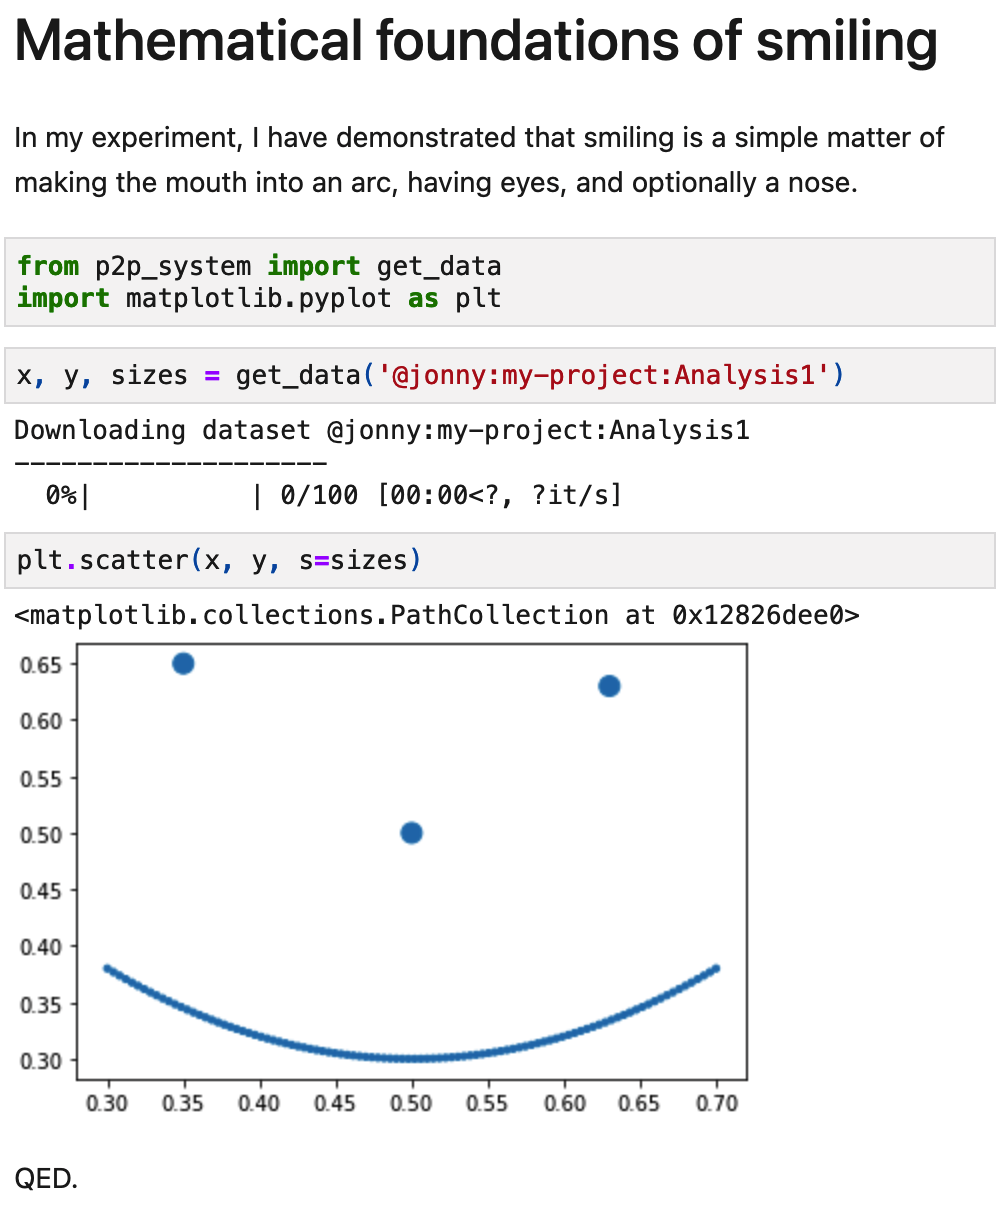
\includegraphics[width=\linewidth]{./images/smile.png}
\label{fig:smilenotebook}
\caption{An example notebook where we use some data loading framework that embeds the linked dataset in the loading cell's metadata field and then plot it!}
\end{figure}

\clearpage

Our notebook file would then include an array of JSON objects that
describe the contents of its cells. For example, our data loading cell
would look something like this:

\begin{Shaded}
\begin{Highlighting}[]
\FunctionTok{\{}
   \DataTypeTok{"cell\_type"}\FunctionTok{:} \StringTok{"code"}\FunctionTok{,}
   \DataTypeTok{"execution\_count"}\FunctionTok{:} \DecValTok{2}\FunctionTok{,}
   \DataTypeTok{"id"}\FunctionTok{:} \StringTok{"rapid{-}information"}\FunctionTok{,}
   \DataTypeTok{"metadata"}\FunctionTok{:} \FunctionTok{\{}
    \DataTypeTok{"scrolled"}\FunctionTok{:} \KeywordTok{true}
   \FunctionTok{\},}
   \DataTypeTok{"outputs"}\FunctionTok{:} \OtherTok{[}
    \StringTok{"..."}
   \OtherTok{]}\FunctionTok{,}
   \DataTypeTok{"source"}\FunctionTok{:} \OtherTok{[}
    \StringTok{"x, y, sizes = get\_data(\textquotesingle{}@jonny:my{-}project:Analysis1\textquotesingle{})"}
   \OtherTok{]}
\FunctionTok{\}}
\end{Highlighting}
\end{Shaded}

The \texttt{"outputs"} description has been abbreviated above, but it
describes to the jupyter notebook server
\href{https://ipywidgets.readthedocs.io/en/latest/examples/Widget\%20Low\%20Level.html}{how
to display it}. Regular text piped through
\href{https://en.wikipedia.org/wiki/Standard_streams}{stdout} is
represented like this:

\begin{Shaded}
\begin{Highlighting}[]
\FunctionTok{\{}
  \DataTypeTok{"name"}\FunctionTok{:} \StringTok{"stdout"}\FunctionTok{,}
  \DataTypeTok{"output\_type"}\FunctionTok{:} \StringTok{"stream"}\FunctionTok{,}
  \DataTypeTok{"text"}\FunctionTok{:} \OtherTok{[}
    \StringTok{"Downloading dataset @jonny:my{-}dataset}\CharTok{\textbackslash{}n}\StringTok{"}\OtherTok{,}
    \StringTok{"{-}{-}{-}{-}{-}{-}{-}{-}{-}{-}{-}{-}{-}{-}{-}{-}{-}{-}{-}{-}}\CharTok{\textbackslash{}n}\StringTok{"}
  \OtherTok{]}
\FunctionTok{\}}
\end{Highlighting}
\end{Shaded}

And multiple output types can be combined in a single cell, for example
a widget like our loading progress bar is described like this:

\begin{Shaded}
\begin{Highlighting}[]
\FunctionTok{\{}
  \DataTypeTok{"data"}\FunctionTok{:} \FunctionTok{\{}
    \DataTypeTok{"application/vnd.jupyter.widget{-}view+json"}\FunctionTok{:} \FunctionTok{\{}
      \DataTypeTok{"model\_id"}\FunctionTok{:} \StringTok{"5799ac2959084a4596ffbad3f9940f48"}\FunctionTok{,}
      \DataTypeTok{"version\_major"}\FunctionTok{:} \DecValTok{2}\FunctionTok{,}
      \DataTypeTok{"version\_minor"}\FunctionTok{:} \DecValTok{0}
    \FunctionTok{\},}
    \DataTypeTok{"text/plain"}\FunctionTok{:} \OtherTok{[}
      \StringTok{"  0\%|          | 0/100 [00:00\textless{}?, ?it/s]"}
    \OtherTok{]}
    \FunctionTok{\},}
    \DataTypeTok{"metadata"}\FunctionTok{:} \FunctionTok{\{\},}
  \DataTypeTok{"output\_type"}\FunctionTok{:} \StringTok{"display\_data"}
\FunctionTok{\}}
\end{Highlighting}
\end{Shaded}

where the \texttt{model\_id}, \texttt{version\_major}, and
\texttt{version\_minor} describe which rendering code to use for the
cell, similarly to the ``metadata that indicates code'' that we
discussed in \protect\hyperlink{analytical-frameworks}{analytical
frameworks}.

Notice that there is already a metadata field! In order to link our
notebook to our analysis --- and thus to our extended graph of data,
experiment, etc. --- we could do it
\href{https://jupyterbook.org/en/stable/content/metadata.html}{manually},
but since we're thinking about interfaces we can also imagine that our
\texttt{p2p\_framework} is capable of filling it in for us. We don't
need to invent a new metadata protocol for JSON,
\href{https://json-ld.org/}{JSON-LD} is already quite similar to the
syntax we've been using already. For simplicity, say we use a
\texttt{@comms} ontology to denote various features of our communication
system. Our data loading function might then populate a field in our
cell like this:

\begin{Shaded}
\begin{Highlighting}[]
\ErrorTok{"metadata":} \FunctionTok{\{}
  \DataTypeTok{"scrolled"}\FunctionTok{:} \KeywordTok{true}\FunctionTok{,}
  \DataTypeTok{"@comms:usesData"}\FunctionTok{:} \StringTok{"@jonny:my{-}project:Analysis1"}
\FunctionTok{\}}
\end{Highlighting}
\end{Shaded}

Other frameworks might make their own metadata annotations, like an
indication that we're plotting some feature of the data, or performing
some statistical analysis on the data. These annotations might be
responsive to the parameterization of the function call or its results,
but if we emphasize a design process that makes interfaces at multiple
levels we could also imagine using something like iPython
``\href{https://ipython.readthedocs.io/en/stable/interactive/magics.html}{magic
commands}'' to declare metadata for our cell. For example, each cell is
automatically assigned a random combination of words as an ID, but if we
wanted to be able to specifically refer to a cell we could give it an
explicit one:

\begin{verbatim}
%%meta @comms:cellID smilePlot
plt.scatter(x, y, s=sizes)
\end{verbatim}

We're familiar with two types of cells, code and markdown, but we can
extend our thinking to arbitrary cell types. What is a cell? A cell has
a a) \textbf{type} that indicates its capabilities and representation,
b) \textbf{metadata} that describes it, we can also generalize that to
include \emph{arguments} that parameterize it, and c) the content, or
information contained by the cell. The jupyter
\href{https://jupyterlab.readthedocs.io/en/stable/api/classes/cells.cellmodel-1.html}{document
model} more or less reflects this already, but in its base model only
has
\href{https://jupyterlab.readthedocs.io/en/stable/api/classes/cells.codecellmodel-1.html}{code},
\href{https://jupyterlab.readthedocs.io/en/stable/api/classes/cells.markdowncellmodel.html}{markdown},
and
\href{https://jupyterlab.readthedocs.io/en/stable/api/classes/cells.rawcellmodel.html}{raw}
cell types, and the metadata field is unstructured. Its extension system
allows for additional cell types as well as restructuring the program
more generally, but since we're focused on self-contained documents
we'll limit our discussion to additional cell types.

From this it's relatively trivial to imagine additional cell types that
serve common needs in academic writing: a citation cell type\sidenote{The
  original Jupyter Notebook paper describes the need for this near the
  end \citep{kluyverJupyterNotebooksPublishing2016}.} that takes
a \href{http://www.bibtex.org/Format/}{BibTeX} object (or its fields) as
arguments and then preserves the full metadata as well as renders it in
a chosen style. A figure cell type that takes an image or plot and a
caption. A contributor cell type that takes an author's name,
affiliation, ORCID, email, and so on. Currently jupyter extensions use
the NPM registry, but we could imagine being able to use other people's
cell types directly by referring to them like
\texttt{@jonny:celltypes:citation}.

Notebooks have multiple levels of metadata, so we can also specify
document-level metadata that describe the type of our document (like a
\href{https://schema.org/ScholarlyArticle}{\texttt{@schema:ScholarlyArticle}}),
its
\href{https://schema.org/creativeWorkStatus}{\texttt{creativeWorkStatus}}
as a \texttt{Draft}, our authorship information, permissions, and
whatever else we'd like. But what is a document? In the case of our
jupyter notebook, it's a series of cell descriptions in a JSON array.
Trivially, a document is a cell that contains other cells. What about in
the other direction? The contents of our cells are \emph{also} a
cell-like system. The very notion of a programming language is a means
of mapping structured syntax to machine instructions, and to do that
code (in some languages) is interpreted or compiled by parsing it into
an \href{https://en.wikipedia.org/wiki/Abstract_syntax_tree}{abstract
syntax tree} that relates data and its structuring metadata. Markdown
can also be thought of as a series of subcells, where using a
\texttt{\#\ header} indicates how the text is to be represented as
compared to \texttt{*italic*} text or
\texttt{{[}links{]}(https://link.com)}. The use of a programming
language or markup syntax is represented by the \texttt{cell\_type}
field, which the notebook server knows to translate \texttt{"code"} to
mean Python and \texttt{"markdown"} to mean its particular flavor of
markdown (of which there are
\href{https://www.iana.org/assignments/markdown-variants/markdown-variants.xhtml}{several}).

This points towards a model of \textbf{recursive} cells that can contain
other cells. An editor could, for example, draw from templating engines
like \href{https://shopify.github.io/liquid/}{liquid}, where an abstract
representation of the content of a cell could include a
\texttt{\{\{\ content\ \}\}} marker that indicates that additional cells
can be included inside of it. Recursive models, coupled with structuring
metadata that indicates the relationship between a parent and child cell
could then be used to model compound concepts. Another simple example
using citation might be to have a cell with one child cell containing a
reference to another work that ours
\href{https://sparontologies.github.io/cito/current/cito.html\#d4e449}{\texttt{@cito:disagrees\_with}}
\citep{peroniFaBiOCiTOOntologies2012}, and another child cell
that in turn contains some writing in markdown and a plot. Recursive
cells also naturally lend themselves to \textbf{transclusion} by making
each of the individual subcomponents of a document referenceable with
full granularity. We will expand on both compound concepts and
transclusion in a moment in talking about the extension of our cellular
system to \protect\hyperlink{trackers-clients--wikis}{wikis}.

Before we go beyond a document system that would be unrecognizable to
most scientists, and thus yet another nice pipedream, it's important to
pause on the continuity with existing document systems. Microsoft Word,
or Word-like WYSIWYG editors like
\href{https://www.libreoffice.org/}{LibreOffice} or Google docs are the
dominant mode of preparing academic documents. Word-like editors are
\emph{already} create recursive cell-like documents, though their
interface obscures them. They support semantic markup like heading
styles (though their use compared to manual formatting is far from
universal \citep{sorgaardUseParagraphStyles1996}), and every
paragraph can be considered a cell, with the default paragraph styling
as its metadata and additional styled elements like bolded words as
sub-cells. It should then be possible to import existing word documents
into a cellular document system. Care should also be taken to smooth the
cognitive transition from word-like editors: Jupyter currently treats
cells as being strictly separate, and new cells need to be created
manually. Instead it should be possible for cells to ``recede into the
background'' and be created with common gestures like a double return to
make a new paragraph. The ``insert'' menu used to create things like
tables or images is already a familiar tool in word-like editors, so the
notion of adding elaborated types like citations shouldn't be that big
of a lift.

The other major document preparation tool modalities are markup syntaxes
and their associated builders like LaTeX. Though TeX-like tools have an
exceedingly opinionated and obscure design history \citep{knuthTeXbook1986}, they have three major affordances: 1)
document-level structure provided by document classes, packages, and the
options they provide, 2) environments that enclose some section of text
between \texttt{\textbackslash{}begin\{\}} and
\texttt{\textbackslash{}end\{\}} and provide some specific functionality
or formatting like
\href{https://www.overleaf.com/learn/latex/Lists}{lists}, and 3)
commands that accept arguments and modify some smaller unit of text like
creating a link with
\texttt{\textbackslash{}href\{https://url.com\}\{link\ text\}}. Each of
these maps onto a cellular document system, with document-level metadata
or the templates commonly used to render markdown, and cells that take
arguments to approximate environments and commands. Markdown extensions
like \href{https://myst-parser.readthedocs.io/en/latest/}{MyST} \citep{dupreAdvertisingNewInfrastructures2022}  make this translation
even more straightforward with direct analogies to LaTeX commands and
environments and their ``role'' and ``directive'' counterparts in
\href{https://www.sphinx-doc.org/en/master/usage/restructuredtext/basics.html}{reStructuredText}.
Since the goal should be a 1:1 relationship between source code and
visual editor, the difference between representing a cell visually
versus in markup should be left as a matter of author preference.

Bidirectional translation from a WYSIWYG editor to its markup is not a
trivial task --- the mediawiki team started writing theirs in
\href{https://www.mediawiki.org/wiki/VisualEditor}{2011} and rolled it
out as a default feature in
\href{https://en.wikipedia.org/wiki/MediaWiki_version_history}{2020}
\citep{forresterInventingWeGo2012}. It's a careful balance
between ease of use, power of syntax, and accomodation of historical
usage patterns. Markdown is on one extreme of ease with only a handful
of markup elements to learn, but has a relatively steep learning curve
to do anything more complex. On the other end is the wonderful
\href{https://dokie.li/}{dokieli} \citep{capadisliDecentralisedAuthoringAnnotations2017}  (and see Sarven's
\href{https://csarven.ca/linked-research-decentralised-web}{masterpiece}
\citep{capadisliLinkedResearchDecentralised2019}, spiritual
cousin to this document), which does essentially everything that we want
our linked documents to do, but requires authors to write their
documents in HTML and manually manage the semantic markup. Extending
Notebooks to use recursive cells with reusable types sacrifices some of
the ability to directly edit the source of a document as a potential way
to balance familiarity and expressiveness.

Notebooks, with some architectural and interfaces then become a
straightforward way of breaking up the scientific paper as a singular
unit of knowldge work when embedded in a linked data system. Their use
in scholarly publishing has been proposed many times before, but our
linking system lets us resolve some of the largest outstanding
limitations \citep{chattopadhyayWhatWrongComputational2020} :
dependency management \citep{ruleTenSimpleRules2019}, archiving
\citep{woffordJupyterNotebooksDiscovery2020}, and discovery,
among others. The same gradient of access control rules we discussed in
controlling access to sensitive data would support a process of gradual
publication of smaller units of work, from a private demo in our lab
meeting to a public part of scientific discourse.

What happens when we invite other people to respond?

\hypertarget{forums-feeds}{%
\subsubsection{Forums \& Feeds}\label{forums-feeds}}

What if we think of our documents as ``threads'' and their cells as
``posts?'' What makes a cellular document a document is some (relatively
arbitrary) notion of a `root' cell that contains the others --- ie. for
notebooks a JSON array of cells. That could be trivially reformulated as
cells with metadata indicating that they are
\href{https://schema.org/isPartOf}{\texttt{PartOf}} a document, each
indicating their \href{https://schema.org/position}{\texttt{position}}
or linked to the cells they are before and after. If we also allow cells
to be
\href{https://www.w3.org/TR/activitystreams-vocabulary/\#dfn-inreplyto}{\texttt{inReplyTo}}
each other, we have the basis of a threaded communication system
continuous with documents. Where cells in a linear document have at most
one preceding and succeeding cell, multiple replies allow a tree
structure that maps onto the patterns of most contemporary social media.
Metadata that describes category and content extends this to include the
structure of forums, and could be the basis of a rich continuum of media
spanning order and chaos, permanence and ephemerality, between the
\emph{magnum opus} and the shitpost: media absent but sorely needed in
academic communication.

Traditional forums like \href{https://www.phpbb.com/}{phpBB} and
contemporary social media operate from a single host with a fixed
interface and representation of posts. What would a communication system
that decouples hosting, identity, interface, and format look like? We
can draw inspiration from the
``\href{https://en.wikipedia.org/wiki/Fediverse}{fediverse},'' a
collection of interoperable software platforms and protocols. The
fediverse makes it possible to communicate across radically different
interfaces: someone using \href{https://funkwhale.audio/}{Funkwhale},
which resembles music software like spotify, can communicate with people
on \href{https://joinpeertube.org/}{PeerTube}, a p2p video streaming
program like YouTube, and \href{https://joinmastodon.org/}{Mastodon}, a
microblogging medium like Twitter. Rather than a single host, instances
of each of these programs are hosted independently and can choose to
federate with other instances to enable communication between them. Most
of these programs use the
\href{https://www.w3.org/TR/2018/REC-activitypub-20180123/}{ActivityPub}
\citep{Webber:18:A}  protocol, which defines a standard set of
capabilities for client-server and server-server communication.

Mastodon posts (or ``toots'') already resemble the kind of
document-interoperable medium hinted at above. For example
\href{https://web.archive.org/web/20220708215201/https://social.coop/@jonny/107328829457619549}{this
post} is represented in (abbreviated) JSON\sidenote[][6cm]{Leaving in this string escaping its box because I think it's sort of cute}:

\begin{Shaded}
\begin{Highlighting}[]

\FunctionTok{\{}
  \DataTypeTok{"to"}\FunctionTok{:}\OtherTok{[}
    \StringTok{"https://www.w3.org/ns/activitystreams\#Public"}
  \OtherTok{]}\FunctionTok{,}
  \DataTypeTok{"cc"}\FunctionTok{:}\OtherTok{[}
    \StringTok{"https://social.coop/users/jonny/followers"}
  \OtherTok{]}\FunctionTok{,}
  \DataTypeTok{"id"}\FunctionTok{:} \StringTok{"107328829457619549"}\FunctionTok{,}
  \DataTypeTok{"created\_at"}\FunctionTok{:} \StringTok{"2021{-}11{-}23T22:52:49.044Z"}\FunctionTok{,}
  \DataTypeTok{"in\_reply\_to\_id"}\FunctionTok{:} \StringTok{"107328825611826508"}\FunctionTok{,}
  \DataTypeTok{"in\_reply\_to\_account\_id"}\FunctionTok{:} \StringTok{"274647"}\FunctionTok{,}
  \DataTypeTok{"visibility"}\FunctionTok{:} \StringTok{"public"}\FunctionTok{,}
  \DataTypeTok{"url"}\FunctionTok{:} \StringTok{"https://social.coop/@jonny/107328829457619549"}\FunctionTok{,}
  \DataTypeTok{"content"}\FunctionTok{:} \StringTok{"\textless{}p\textgreater{}and making a reply to the post to show the in\_reply\_to and context fields\textless{}/p\textgreater{}"}\FunctionTok{,}
  \DataTypeTok{"account"}\FunctionTok{:}
  \FunctionTok{\{}
      \DataTypeTok{"id"}\FunctionTok{:} \StringTok{"274647"}\FunctionTok{,}
      \DataTypeTok{"username"}\FunctionTok{:} \StringTok{"jonny"}\FunctionTok{,}
      \DataTypeTok{"fields"}\FunctionTok{:}
      \OtherTok{[} \ErrorTok{...} \OtherTok{]}
  \FunctionTok{\},}
  \DataTypeTok{"media\_attachments"}\FunctionTok{:} \OtherTok{[]}\FunctionTok{,}
  \DataTypeTok{"mentions"}\FunctionTok{:} \OtherTok{[]}\FunctionTok{,}
  \DataTypeTok{"tags"}\FunctionTok{:} \OtherTok{[]}\FunctionTok{,}
\FunctionTok{\}}
\end{Highlighting}
\end{Shaded}

As described
\protect\hyperlink{for-making-our-peers-and-the-links-within-their-namespace-discov}{previously},
ActivityPub supports linked data with JSON-LD -- a remarkable feat
despite the justifiable angst with the protocol \citep{kaniiniActivityPubPresentState2019, schubertActivityPubFinalThoughts2019}  given the historical grudges between linked data and indieweb
communities (See this retrospective by one of its authors, Christine
Lemmer-Webber \citep{lemmer-webberStandardsDivisionsCollaboration2018}). So we could imagine that post using a reference to a document or
one of its cells in its \texttt{in\_reply\_to} field.

Mastodon might be a good transitional medium, but we can extend it to
make use of our linked p2p system. The fediverse decouples the network
from a single platform, but instances still bundle together the
underlying data of a post with an interface, host, and account (but see
\href{https://hubzilla.org//page/hubzilla/hubzilla-project}{hubzilla}).
p2p helps us decouple accounts from hosts (see this discussion on a p2p
ActivityPub \citep{webberActivityPubDecentralizedDistributed2017}), but we would also like to decouple interfaces from the underlying
data so that we have a continuous communication medium where different
interfaces are just \emph{views} on the data. To do that we would want
to start by replacing Mastodon's flat ``\texttt{content}'' field with
the kind of typed cells in our documents that indicate what kind of
message they are. For example a simple text-based message might use the
ActivityStreams
\href{https://www.w3.org/TR/activitystreams-vocabulary/\#dfn-note}{\texttt{Note}}
type:

\begin{Shaded}
\begin{Highlighting}[]
\FunctionTok{\{}
  \DataTypeTok{"@context"}\FunctionTok{:} \StringTok{"https://www.w3.org/ns/activitystreams"}\FunctionTok{,}
  \DataTypeTok{"type"}\FunctionTok{:} \StringTok{"Note"}\FunctionTok{,}
  \DataTypeTok{"name"}\FunctionTok{:} \StringTok{"My Message"}\FunctionTok{,}
  \DataTypeTok{"content"}\FunctionTok{:} \StringTok{"A note I send to you!"}
\FunctionTok{\}}
\end{Highlighting}
\end{Shaded}

But we might equivalently send a \texttt{@jupyter:Notebook} as a
message, or some compound object like a
\href{https://www.w3.org/TR/activitystreams-vocabulary/\#dfn-collection}{\texttt{Collection}}:

\begin{Shaded}
\begin{Highlighting}[]
\FunctionTok{\{}
  \DataTypeTok{"@context"}\FunctionTok{:} \StringTok{"https://www.w3.org/ns/activitystreams"}\FunctionTok{,}
  \DataTypeTok{"summary"}\FunctionTok{:} \StringTok{"A Compound Message!"}\FunctionTok{,}
  \DataTypeTok{"type"}\FunctionTok{:} \StringTok{"Collection"}\FunctionTok{,}
  \DataTypeTok{"totalItems"}\FunctionTok{:} \DecValTok{2}\FunctionTok{,}
  \DataTypeTok{"items"}\FunctionTok{:} \OtherTok{[}
    \FunctionTok{\{}
      \DataTypeTok{"type"}\FunctionTok{:} \StringTok{"Note"}\FunctionTok{,}
      \DataTypeTok{"name"}\FunctionTok{:} \StringTok{"Hey how ya doin here\textquotesingle{}s a notebook"}
    \FunctionTok{\}}
    \FunctionTok{\{}
      \DataTypeTok{"@context"}\FunctionTok{:} \StringTok{"https://jupyter.com/"}\FunctionTok{,}
      \DataTypeTok{"type"}\FunctionTok{:} \StringTok{"Notebook"}\FunctionTok{,}
      \DataTypeTok{"content"}\FunctionTok{:} \StringTok{"..."}
    \FunctionTok{\}}\OtherTok{,}
  \OtherTok{]}
\FunctionTok{\}}
\end{Highlighting}
\end{Shaded}

So the \emph{existence} of a particular type of message is not bound to
the ability of any given program's ability to render it. Our notebook
program might not be able to understand what it means to have people
responding to and making threads about its cells, but we would still be
able to receive them and open them with an interface that does, and we
could further imagine the ability for a type to recommend a program to
us for rendering it as we did with the ability for analysis nodes to
specify the code to execute them. We will set aside for a moment the
issues of moderation and permission for which messages can link to our
work and the practicalities of sending, receiving, storing, and serving
messages and return to them in the context of
\protect\hyperlink{overlays--adversarial-interoperability}{annotations}
and \protect\hyperlink{trackers-clients--wikis}{trackers}, respectively.

\emph{Where} do our posts go? For concreteness, we can start with a
forum called ``NeuroChat.'' \texttt{@neurochat} is a peer like any
other, and it supports some of the basic ActivityStreams vocabulary. We
can request to join it by sending a
\href{https://www.w3.org/TR/activitystreams-vocabulary/\#dfn-join}{\texttt{@as:Join}}
request, which gives it permission to index our public posts and issue
links on our behalf through its web interface. It has a few broad
categories like ``Neuromodulation'' and ``Sensory Neuroscience,'' within
which are collections of threads full of chronologically-sorted posts.
Threads are objects that indicates a category like
\texttt{@neurochat:categories:Neuromod}, and when we post in them we
create links that are
\href{https://www.w3.org/TR/activitystreams-vocabulary/\#dfn-attributedto}{\texttt{@as:attributedTo}}
us with the
\href{https://www.w3.org/TR/activitystreams-vocabulary/\#dfn-context}{\texttt{@as:context}}
of the thread we're posting in and any
\href{https://www.w3.org/TR/activitystreams-vocabulary/\#dfn-inreplyto}{\texttt{@as:inReplyTo}}
links to preceding or quoted posts.

We want to announce and describe some recent results in our document
\texttt{@jonny:my-project:Writeup}. This kind of post is common in
\texttt{@neurochat}, and so instead of a generic citation we use a
\texttt{@neurochat:AnnouncesResult} link to indicate the relevant
document. In our forum pseudocode we'll use a \texttt{\#prefix} macro to
give a short name to our project and semantic wikilinks with a
\texttt{{[}{[}predicate::object{]}{]}} syntax for the purpose of
demonstration, though ideally these would be part of the forum's
interface. We think we really have something that challenges some widely
held previous results:

\begin{Shaded}
\begin{Highlighting}[]
\NormalTok{\#prefix project @jonny:my{-}project }
\NormalTok{\#prefix nc @neurochat}

\NormalTok{Hi everyone, happy to present my new work}
\NormalTok{[[nc:AnnouncesResult :: project:Writeup]].}

\NormalTok{I think it raises a number of interesting questions,}
\NormalTok{in particular @rival\textquotesingle{}s longstanding argument}
\NormalTok{[[@cito:disputes :: @rival:TheBrainIsInTheLiver]].}

\NormalTok{I also wonder what this means about the conversation}
\NormalTok{we\textquotesingle{}ve been more generally about}
\NormalTok{[[@cito:discusses :: @discipline:whereAreTheOrgans]].}

\NormalTok{Anyway, write back soon, xoxo.}
\end{Highlighting}
\end{Shaded}

Our rival takes the criticism in stride but wants to run their own
analysis. They follow the links back to find our data, and reanalyze it.
Their analysis framework has already issued a link indicating that it
reanalyzes our data, and rather than do an independent writeup our rival
returns to the thread to continue the discussion.

\begin{Shaded}
\begin{Highlighting}[]
\NormalTok{Interesting result, you old scoundrel. }

\NormalTok{That indeed [[disputes :: @doi:\textless{}id\textgreater{}]],}
\NormalTok{in particular its section [[.:results:main]]}
\NormalTok{and my re{-}analysis adds another wrinkle to the problem!}
\NormalTok{Take a look:}

\NormalTok{[[nc:embed :: @rival:reanalysis]]}

\NormalTok{This really complicated another project of mine,}
\NormalTok{[[@rival:projects:NeuronsCanSwim]]}
\end{Highlighting}
\end{Shaded}

Our forum's \texttt{embed} link knows how to embed the notebook our
rival used to do their reanalysis and in the underlying message
indicates the the current version so if they update it in the future the
message will still be comprehensible. Our rival doesn't use a predicate
for their link to their side-project and our forum uses its default
\texttt{Mentions} predicate. It's still more informative than a duplet
link because the context of being a discussion in our forum the links in
the surrounding posts. We could imagine additional capabilities we give
to our forum, like the ability to automatically trigger a re-analysis by
someone mentioning a different pipeline for a given dataset, but we'll
leave those as an exercise to the reader.

This example is a relatively trivial instance of scientific
communication: sharing results, relating them to previous findings, and
thinking about the broader implications on the field. However in our
current regime of scientific communication, even in the most progressive
publication venues that allow communication directly on a work, this
kind of communication is \emph{entirely invisible} to the broader state
of our understanding. With our system of linked communication, however,
the entire provenance chain from our experiment through its analysis and
contextualizing discussion is related to immediately related work as
well as the standing questions in our field. Our work is enriched by the
additional analysis from our rival, and their work is continuously
contextualized as the state of our understanding develops. We were
capable of making incremental refinements to our shared understanding
using units of work that were much smaller than the traditional
scientific paper. It would be possible for someone entirely outside our
field to browse through the general links from basic research questions
to relevant work and its surrounding discussion. If they were to ask
questions, our answers would represent the latent diffusion of
understanding to other disciplines based on the graph context of our
respective work --- and we could be credited the time we spent doing so!
In short, scientific communication could actually be \emph{cumulative.}

Forums are just one point in a continuous space of threaded media. If we
were to take forum threads out of their categories, pour them into our
water supply, and drink whatever came our way like a dog drinking out of
an algorithmic fire hydrant, we would have Twitter. Remove the algorithm
and arrange them strictly chronologically and we have Mastodon. In both,
the ``category'' that organizes threads is the author of the initial
post. Algorithmic, rather than purposefully organized threaded systems
have their own sort of tachycardic charm. They are effective at what
they aim to do, presenting us whatever maximizes the amount of time we
spend looking at them in a sort of hallucinatory timeless now of
infinite disorganization --- at the expense of desirable features of a
communication system like a sense of stable, autonomously chosen
community, perspective on broader conversation, and cumulative
collective memory.

Nevertheless the emergence of a recognizable ``Science Twitter'' points
towards a need for relatively informal all-to-all communication.
Serendipitously being able to discover unlikely collaborators or ideas
is a beautiful dream, if one ill-served by the for-profit attention
economy. Our formulation of the \texttt{@neurochat} forum was as an
equal peer that mirrored, collected, and organized posts that otherwise
are issued from other peers such as ourselves. In the same way that we
might use the ActivityStreams \texttt{Join} action to have our posts
mirrored by it, we might also use
\href{https://www.w3.org/TR/activitystreams-vocabulary/\#dfn-follow}{\texttt{@as:Follow}}
to receive posts from any peer, and in the case of a federation that
might include posts from its members sent to the federation. Notice in
the example mastodon post above how it uses JSON-LD and the
activitystreams ontology: a ``me to the world'' tweetlike message is
addressed to \texttt{activitystreams\#Public} and cc'd to the URL that
corresponds symbolically to the list of \texttt{@jonny}'s followers.

We can take advantage of the graph structure and rich metadata of our
social network in ways that are impossible in corporate social media
networks that require the expectation of disorder to be able to sell
``native'' ad placement. The instance-to-instance federation model of
the fediverse, and the accompanying absence of any ``global'' scope of
all posts, results in the need for multiple views on the network: in
Mastodon, a ``local'' timeline that shows only posts from within the
host instance, and a ``federated'' timeline that shows posts from all
instances that the host instance has federated with. Since our network
allows peer-to-peer, federation-to-federation, and peer-to-federation
interaction, we can extend that further. We can construct views of the
network based on granular control over graph depth: instead of seeing
just the posts from the peers that we follow, we can request to see
n-depth posts, from the peers that our peers follow, and so on. This
could be done at the level of a ``view'' or at the level of the follow
link itself --- since I know this person well, I want to see a graph
depth of 2 from them, and a depth of 1 from others. At the federation
level, we might imagine that \texttt{@neurochat} is federated with
another \texttt{@linguisticsChat} group and the two mirror and rehost
each other's posts. We could then make use of our extended social graph
and prioritize posts from people who are part of overlapping subsets of
the federations we are a part of. The peer-based nature of our social
network serves as the basis for a system of fluid scoping and filtering
of the kind of communication we are looking for at any given time. So
rather than a disorganized public melee or the empty rooms and new
logins from yet another closed Slack, our communication could be part of
a coherent scientific conversation.

Across from filtering what we receive, the same could be done to what we
send by choosing where our posts are addressed and who can see them. The
same multimodality of ``following'' used to indicate the graph depth of
the posts we see could let us indicate different kinds of relationships.
We should be able to send global, undirected messages on a public feed,
but we don't necessarily want to talk to our friends in the same way
that we talk to strictly professional colleagues. We might want to
organize privately with a few colleagues, or prevent trolls or hostile
groups from accessing or making use of our work. Effectively, we should
be able to direct our messages to different groups of peers to support
the multiple registers of our communication.

The need for rapid and informal scientific communication being mediated
by corporate social networks has the unfortunate byproduct of needing to
carefully manage a ``personal brand.'' To be seen as a ``serious,'' we
need to maintain some proximity to the stilted academic voice,
forfeiting any approachability to science that might be gained from
public communication. If we are to expand the scope of what we consider
as the labor of scientific communication, we should also take seriously
its many registers and contexts. Informal media like alt accounts,
mailing lists, groupchats, zines, and whisper networks are also an
integral part of science, particularly for marginalized and vulnerable
scientists \citep{jimenezBorderlandingAcademicResearchers2020}.
Parallel to organizing our communication in empirical professional
communication, we might build systems that support our organization into
federations to more effectively bargain over our working conditions and
protect ourselves. The venues that organize our communication being
limited to journals, and the accompanying regulation over the registers
of communication that count as ``real'' science, is even more limiting
than its profound effects on scientific literature proper. The absence
of infrastructure to support the multiregister communication of science
limits our ability to organize over the broader state of our work, form
extended communities, and reduces what should be the collective project
of making our work broadly understandable to the individualistic
projects of ``scicomm influencers.'' It shouldn't take a lot of
additional critical analysis to say ``shitposts are good, actually, for
science.''

There's a balance to be struck between a system of granular control over
the messages we send and receive with the ease of a monolithic
algorithmic feed. Mastodon sorts all posts purely chronologically, which
translates into relatively steep limits on the size of communities as
feeds become unintelligible washes of posts. Instead of forgoing
algorithmic organization altogether, another means by which we could
take advantage of the graph structure of our network is by being able to
\emph{choose} the sorting algorithms we use. We might want to prioritize
posts from someone who we don't necessarily follow but is interacting
with people that we do in contexts that we share, or be able to
deprioritize posts that are ``close'' to us in our social graph in order
to discover new things. This too could be a cumulative, community-driven
project, where we might want to try out our friend's
\texttt{@friends:sorting:NewAlgorithm}, tweak it a bit for our
preferences, and republish a new version.

Generally, the impact of having a communication system that decouples
hosting, identity, interface, and format on an underlying linked data
graph gives us a broad space to build different views and tools to use
the underlying data. Specifically, without predicting the infinite
future of communication media, our system of linked, cell-like
communication generalizes threadlike media like forums and feeds into a
continuous system that can blend their features as needed. Durable,
cumulative discussion about the state of our understanding should be
able to live side-by-side with ephemeral, informal conversations. It
should be possible for us to serendipitously discover people and
information as well as for a newcomer to have a place to ask questions
and build their understanding. It should be possible for us to form and
dissolve communities fluidly without substantial technical start-up
costs and the total loss of memory when they close. A system that
supports the fullness of continuous communication would be an
unfathomably richer way of building reliable, accessible, and
multivalent understanding of our reality than the current system of a
gladitorial thumbs up/down indictment on years of your life that is
journal-based peer review.

\hypertarget{overlays-adversarial-interoperability}{%
\subsubsection{Overlays \& Adversarial
Interoperability}\label{overlays-adversarial-interoperability}}

We can't expect the entire practice of academic publishing to transition
to cell-based text editors in a p2p linked data swarm overnight. In the
same way that we discussed frameworks for integrating heterogeneous
analytical and experimental tools, we need some means of
\textbf{bridging} communication tools and \textbf{overlays} for
interacting with existing communication formats. There are many examples
of bridging communication protocols, eg. the
\href{https://matrix.org/bridges/}{many ways to use Matrix} with
\href{https://matrix.org/bridges/\#slack}{Slack},
\href{https://matrix.org/bridges/\#email}{email},
\href{https://matrix.org/bridges/\#signal}{Signal}, etc. The overlays
for websites, pdfs, and other more static media that we'll discuss are
means to bring them into the system whether they support it or not: our
interoperability should be willing to be adversarial if it needs to be
\citep{doctorowAdversarialInteroperabilityReviving2019, doctorowAdversarialInteroperability2019}. In representing the
intrinsically interactive and social nature of reading (eg. see \citep{jacksonMarginaliaReadersWriting2001}), overlays as interfaces
also supplement the ``horizontal'' connections between cells by
injecting information into them or transcluding it elsewhere: creating a
fuzzy boundary between writing \emph{on} something vs \emph{about}
something.

We don't need to look far to find a well-trod interface for annotation
overlays for document-like media: the humble highlighter.
\href{https://hypothes.is}{Hypothes.is}, enabled on this page, lets
readers highlight and annotate any webpage with a
\href{https://chrome.google.com/webstore/detail/hypothesis-web-pdf-annota/bjfhmglciegochdpefhhlphglcehbmek}{browser
extension} or javascript bookmarklet. This interface is a near match to
the highlighting and review tools of Microsoft Word and Google Docs used
for the same purpose. At its heart is a system for making anchors,
references to specific places in a text, and the means of matching them
even when the text changes or the reference is ambiguous \citep{csillagFuzzyAnchoring2013}. For example,
\href{https://hypothes.is/a/oLw4uk7_Eeyt5N-FVlE3fw}{this anchor} has
three features, a \texttt{RangeSelector} that anchors it given the
position within the paragraph, an absolute
\texttt{TextPositionSelector}, and a contextual
\texttt{TextQuoteSelector} that you can see with an
\href{https://api.hypothes.is/api/annotations/oLw4uk7_Eeyt5N-FVlE3fw}{API
call}. Anchors like these, along with references to the
\href{https://github.com/hypothesis/client/blob/fb08cdf38191643d7a35d84ca3b822589c2e880a/src/annotator/anchoring/types.js}{code
that resolves them}, could be the objects to which we could link from
the rest of our communication system.

On its own, it serves to give a \texttt{Talk:} page to every website.
With an integration into a system of linked data and identity, it also
serves as a means of extending the notion of bidirectional transclusion
described above to work that is not explicitly formatted for it. Most
scientific work is represented as \texttt{.pdf}s rather than
\texttt{.html} pages, and hypothes.is
\href{https://web.hypothes.is/help/annotating-locally-saved-pdfs/}{already
supports} annotating PDFs. With an integration into pdf reading
software, for example
\href{https://www.zotero.org/support/pdf_reader_preview}{Zotero's PDF
reader}, there would be a relatively low barrier to integrating
collaborative annotation into existing workflows and practices.

Digital publishing makes imagining the social regulation of science as a
much more broadly based and continuous process much easier, but the
problem of moderation remains (as it has since at least the coiner of
the terms ``Gold'' and ``Green'' open access lost faith in ahierarchical
scientific communication after someone said poo-poo words at him on
Internet while defending the use of they/them as gender-ambiguous
pronouns \citep{harnadSkyWriting1987, harnadScholarlySkywritingPrepublication1990, ellisBooksTranslationWanted1986}). Some movement has been made
towards public peer review: eLife has integrated hypothes.is since 2016
\citep{ELifePartnersHypothes2016}, and bioRxiv had decided to
integrate it as well in 2017 \citep{dwhlyBioRxivSelectsHypothesis2017}  before getting cold feet about the genuinely hard problem of
moderation (among others \citep{heatherstainesPreprintServicesGather2018}) and instead adopting the
more publisher-friendly TRiP system of refereed peer-reviews \citep{nateangellAnnouncingTRiPTransparent2019}.

Overlays raise basic questions about control over the representation of
our work, about who is able to write what on it. As with potential
incompatibility between interfaces, we should be able to control what
comments appear \emph{on} our work, but there is no way to control --
even in our current communication systems -- what someone says
\emph{about} it. Our system gives us some ability to identify bad actors
and regulate the avenues of communication without overcorrecting into a
system where criticism becomes impossible -- even if we don't want to
represent someone's comments on our work, it is possible to make them
and for others to find them, but it's also possible to contextualize
their context if they're made in bad faith.

Though a description of the norms and tools needed to maintain healthy
public annotation is impossible here, our system \emph{provides a space
for having that conversation.} Authors could, for example, allow the
display of annotations from a professional society like \texttt{@sfn}
that has a code of conduct and moderation team, or annotations
associated with comments on \texttt{@pubpeer}, or from a looser
organization of colleagues and other \texttt{@neurofriends}. Conversely,
being able to make annotations and comments from different federations
gives us a rough proxy to different registers of communication and
preserves the plurality of our expression. Social tools like these are
in the hypothes.is team's
\href{https://web.archive.org/web/20211015213849/https://github.com/hypothesis/product-backlog/projects/6}{development
roadmap}, but I intend it as a well-developed and mature example of a
general type of technology\sidenote{cf.~the
  \href{https://genius.com}{genius.com} overlay.} rather than a
recommendation.

In addition to annotating other works, overlays can come in the form of
bots or other tools for interacting with existing systems in a way
that's compatible with a new one. One particularly impressive example of
aggressive interoperability in this domain is Eduardo
\href{https://flancia.org/}{``flancian''} Ivanec's
\href{https://anagora.org/}{agora} \citep{ivanecFutureNoteTaking2021, velitchkovPersonalKnowledgeGraphs}. An agora is a
\href{https://anagora.org/wiki-like}{wiki-like} project with pages (or
nodes) for each named concept, but it also allows for multiple
representations of a given node: so notes from multiple people across
multiple mediums will be present on the same page. Accompanying the
agora is the anagora bot (on
\href{https://botsin.space/@agora}{Mastodon} and
\href{https://twitter.com/an_agora}{Twitter}), which makes links to, and
backlinks from pages mentioned as \texttt{{[}{[}wikilinks{]}{]}} by
accounts that follow them (for example: a
\href{https://social.coop/@jonny/108621001205679783}{post}, the bot's
\href{https://botsin.space/@agora/108621001318792297}{reply}, and one of
the linked pages,
\href{https://anagora.org/Wikilinks+Everywhere}{\texttt{{[}{[}wikilinks\ everywhere{]}{]}}}).
This becomes natural quickly: it's common for people associated with the
agora (or \href{https://flancia.org/manifesto/}{flancians}) to speak
with wikilinks, or index links and conversations that they come across
for mutual discovery.

The agora makes linked annotation a basic part of using the web without
requiring fundamental changes in communication practices. The agora is
an exercise in radically permissive protocol-like thinking: rather than
creating a new app or platform, theoretically any bot could be made to
crawl different mediums for wikilinks and index them. It illustrates
that interfaces can precede formal protocols and serve as a testing and
development ground for them.

Another bridging overlay for more author-focused scientific
communication would be to explicitly archive the threads that
increasingly serve as companions to published work --- or original works
of scholarship on their own (eg. \citep{bostonNeedKnowInformationSeeking2022}). I have started experimenting
with this with the
\href{https://twitter.com/threadodo_bot}{\texttt{@threadodo\_bot}}, a
bot that converts a thread to a PDF\sidenote{complete with markdown
  rendering!} and uploads it to Zenodo when it is tagged beneath one.
This bot is being programmed as a
\href{https://github.com/sneakers-the-rat/threadodo/blob/58d5f13f88728babdf2da0b34310c88349725566/threadodo/actions/commands.py\#L145-L168}{generalizable
framework for bots} that can accept parameterized commands. For example,
someone can set their authorship information by tweeting
``\href{https://twitter.com/json_dirs/status/1542305909983936512}{identify}''
at threadodo, which accepts a series of key-value pairs to set your
name, affiliation, and orcid. Future versions will support automatic
reference generation for linked works, including previously archived
threads, as well as setting prefixes for OWL schema for use in semantic
\texttt{{[}{[}predicate::object{]}{]}} wikilinks.

When some recognizably different communication medium begins to
coalesce, it should support bidirectional \emph{crossposting} to and
from existing mediums. Crossposting substantially eases transition ---
for example between
\href{https://crossposter.masto.donte.com.br/}{Twitter and Mastodon} ---
as patterns of usage that have been trained for years on hyperoptimized
attention-capturing platforms are hard to break. Together with bridges,
bots, and overlays for annotation, linking, and archiving, the dream of
rewriting the norms of academic communication looks less like some ``if
you build it they will come'' pipe dream and more like a transitional
period of demonstrating what we can dream of together. Adversarial
interoperability not only \emph{works} \citep{doctorowAdversarialInteroperability2019}, it's also a gift of the
\href{https://www.gwern.net/Unseeing}{hacker mindset} that teaches us
how to make building a better world an act of unrepentant \emph{joy.}

\hypertarget{trackers-clients-wikis}{%
\subsubsection{Trackers, Clients, \&
Wikis}\label{trackers-clients-wikis}}

The final set of social interfaces are those for collective governance
of the system. So far we have generalized documents ``vertically'' into
recursive typed cells, ``horizontally'' into linked cells for
communication, and then blurred their independence by and extended them
into incompatible media with overlays. The remaining piece we need are
multi-authored documents: \textbf{wikis}. We'll pick up the threads left
hanging from our description of
\protect\hyperlink{archives-need-communities}{bittorrent trackers} and
knit them in with those from \protect\hyperlink{the-wiki-way}{the wiki
way} to describe how systems for surfacing procedural and technical
knowledge work can also serve as a basis of searching, indexing, and
governing the rest of the system. Where the rest of our interfaces were
means of creating particular kinds of structured links, we'll also
describe wikis as a means of interacting directly with links to
negotiate the relationships between the multiplicity of our folksonomic
schema. In the process we'll give some structure to the \textbf{clients}
and \textbf{trackers} that serve and organize them.

Our notion of recursive cell-like documents is already a good basis for
wiki pages. \textbf{Multi-author} documents should already be possible
with a permission system that we have invoked previously to limit read
access, and so the most radically open, publicly editable wikis would
just have edit permissions open to anyone. The \textbf{version history}
that makes the notion of
\href{http://meatballwiki.org/wiki/SoftSecurity}{SoftSecurity} possible
should also be a general property of links in our system. The other
concept we'll borrow from traditional wikis is the model where
\textbf{pages represent topics.} Practically, let's suppose this means
that within documents beneath some namespace like \texttt{@jonny:wiki},
we can make wikilinks to {[}{[}New Pages{]}{]} that imply links to
\texttt{@jonny:wiki:New\_Pages} --- though for the sake of simplicity in
this section we will assume that our wiki starts at the root of the
\texttt{@jonny} namespace.

We want to preserve two types of multiplicity: the multiplicity of
\emph{representations} (as in \texttt{Talk:} pages) and \emph{instances}
of a given topic, or the ability for multiple peers to have linked
versions that potentially transclude content from other peers, but are
ultimately independent. Both can use different components of a
namespace: for multiplicity of representation we might follow the
example of mediawiki and use parallel namespaces like
\texttt{@jonny:talk}, and multiplicity of instances follows naturally
from parallel peers by linking \texttt{@jonny:wiki:My\_Page} to
\texttt{@rumbly:wiki:My\_Page}.

Wikis that represent multiple instances of a given page are already a
subject of active experimentation. Flancian's Agora is one example,
which is based on markdown files in git repositories, and markdown files
with the same name in federated repositories are presented on the same
page. A much older project\sidenote{everything2 (or e2) users tend to
  be, uh,
  \href{https://everything2.com/title/Everything\%253A+In+the+Beginning}{floridly
  sarcastic}, and so its history is not as clearly laid out as the other
  old wikilike sites.}, \href{https://everything2.com/}{everything2} is
built around multiple
``\href{https://everything2.com/title/Writeup}{writeups}'' for a given
``\href{https://everything2.com/title/Node}{node}.'' Multiple instances
of a page are also a defining feature of Ward Cunningham's
\href{http://ward.fed.wiki.org/view/welcome-visitors/view/home-in-the-federation}{federated
wiki}, which has a vertical ``strip'' based interface where clicking the
colored squares at the bottom of a given page will open another strip to
show another user's instance of the page. We'll borrow Ward's
terminology and refer to this kind of wiki as a federated wiki.

Federated wikis already have some broader purchase as ``personal
knowledge graphs,'' \citep{balogPersonalKnowledgeGraphs2019} 
where people use tools like \href{https://www.notion.so/}{Notion} or
\href{https://obsidian.md/}{Obsidian} to keep a set of linked,
semistructured personal notes. Rather than thinking of a wiki as
wikipedia, with pages that aspire to be uniformly named and written,
personal knowledge graphs take whatever form is useful to the person
maintaining them. This maps neatly onto our namespaces and recursive
documents as a means of \emph{organizing our system of links.}

Say we have a very simple project structure that consists of a dataset
with two tables and a document with the date of the experiment and some
short description of the data. In our pseudocode:

\begin{Shaded}
\begin{Highlighting}[]
\NormalTok{\textless{}\#project\textgreater{}}
\NormalTok{  a @jonny:Project}

\NormalTok{  dataset}
\NormalTok{    @format:csv }
\NormalTok{      table1}
\NormalTok{      table2}

\NormalTok{  document}
\NormalTok{    a @jupyter:notebook}

\NormalTok{    @schema:Date dateCollected}
\NormalTok{    Description}
\NormalTok{      "This is the data that I collected"}
\end{Highlighting}
\end{Shaded}

This has a natural representation in our wiki as a set of nested cells:
the \texttt{@jonny:project} page has two child cells, one for the
dataset and one for the document, which have their own child cells that
represent the tables, date, and description according to their types.
Since the relationships between our cells can also typed, ie. have an
associated predicate like \texttt{before}, \texttt{after}, or
\texttt{inReplyTo}, we'll use two additional types to differentiate
nested cells:

\begin{itemize}

\item
  \texttt{child} (and its inverse \texttt{parent}) cells correspond to a
  cell's position in our namespace, so we could find our data at
  \texttt{@jonny:project:dataset}.
\item
  \texttt{transcludes} (and its inverse \texttt{transcluded}) indicates
  some other cell that we represent on a given wiki page, as we might
  want to do if we wanted to embed one of our plots in a post.
\item
  And other cells linked with bare \texttt{{[}{[}wikilinks{]}{]}} are
  untyped.
\end{itemize}

This gives us a bidirectional representation of our link structure: and
with it an interface for browsing and managing all the various types of
objects that we have described so far.

Since schemas, or abstract representations of the links a type might
have, are themselves made of links, these too can be managed with a
wiki.
\href{https://www.semantic-mediawiki.org/wiki/Semantic_MediaWiki}{Semantic
mediawiki} and its
\href{https://www.mediawiki.org/wiki/Extension:Page_Schemas}{page
schemas} extension implement a system like this. For example, the
\href{https://wiki.auto-pi-lot.com}{Autopilot wiki} has a
\href{https://wiki.auto-pi-lot.com/index.php/Form:Build_Guide}{form} to
submit build guides for experimental apparatuses. Build guides have a
\href{https://wiki.auto-pi-lot.com/index.php/Category:Construction_Build_Guide}{schema}
and an associated
\href{https://wiki.auto-pi-lot.com/index.php/Template:Build_Guide}{template}
that lays out the form input on the created page and makes the semantic
wikilinks that declare its properties like
\texttt{{[}{[}Is\ Version::2{]}{]}}.

This system is semantically rich while also being flexible, as
everything reduces down to semantic wikilinks on a page, so free text
can be used fluidly along with structured schemas, forms, and templates.
The wide open structuring space of the wiki handles the messy iteration
of technical knowledge work well while also having enough structure to
be computer readable. A page for an
\href{https://wiki.auto-pi-lot.com/index.php/HiFiBerry_Amp2}{amplifier}
makes the datasheet, serial protocol, and the GPIO pins it needs
available via an
\href{https://www.semantic-mediawiki.org/wiki/Help:API}{API call} while
also carrying on a continuous effort to crudely defeat its low-pass
output filter. A
\href{https://wiki.auto-pi-lot.com/index.php/Plugin:Autopilot_Paper}{plugin}
page can credit the papers it was used in by DOI and the python packages
needed to run it while also describing how to void the warranty of your
oscilloscope to unlock additional functionality.

The page-centric model of semantic wikis poses a problem, though. The
guide for building the
\href{https://wiki.auto-pi-lot.com/index.php/Autopilot_Behavior_Box}{Autopilot
Behavior Box} has semantic annotations describing the CAD schematics,
materials, and tools that it uses. This works fine for
\href{https://wiki.auto-pi-lot.com/index.php/Autopilot_Tripoke}{other
assembled parts} or schematics like
\href{https://wiki.auto-pi-lot.com/index.php/Autopilot_Nosepoke_Cap}{3d
printed parts} that have pages of their own, because their pages can
contain the additional properties that describes them like the
associated \texttt{.stl} files. Materials like screws are trickier. Each
screw varies along about a dozen dimensions, and so that either requires
making a separate page for each individual screw or use
workarounds\sidenote{like
  \href{https://www.semantic-mediawiki.org/wiki/Subobject}{subobjects}
  or
  \href{https://www.semantic-mediawiki.org/wiki/Help:Type_Record}{record
  types}} that reduce the maximum depth of representation to two layers
and add other nasty complexities.

A recursive cellular system avoids these problems and provides a uniform
interface to complex representations. We can create schema for
experiments that allow for a build guide, which can contain assembled
component descriptions, which can contain materials, etc. When using
that schema to describe a new experiment, the researcher can be prompted
for any of the possible available fields in the recursive model while
also allowing for free space to write in the semi-structure of the
building blocks. Extending an existing schema is just a matter of
transcluding it and then modifying it as needed. With the ability for
our interface to assign fixed IDs for these objects or generate unique
hashes based on their contents, the tension of ephemeral object
declaration with unique addresses disappears.

The tension of arbitrarily flexible personal knowledge graphs with
multiscale organization with other peers remains, though. Approaching
from the other side of discovery, rather than declaration of information
leads back to considering the structure of our p2p client and
tracker-like systems. The most immediate problem we face is the need to
reconcile the differences between multiple instantiations of overlapping
representations of concepts that change through time. That sounds a lot
like version control system, and a VCS like git or mercurial should be a
natural part of our client. Where IPFS is ``a single bittorrent swarm,
exchanging objects within one Git repository,'' \citep{benetIPFSContentAddressed2014}  we make a mild modification and think
of a single bittorrent swarm with a git repository per peer (also see
\href{https://ipld.io/docs/}{IPLD} \citep{protocollabsIPLDDocs2021}). Git
\href{https://git-scm.com/book/en/v2/Git-Internals-Git-Objects}{stores
files} as
\href{https://en.wikipedia.org/wiki/Content-addressable_storage}{content-addressed}
``blobs'' of binary indexed by ``trees'' that represent the file
hierarchy \citep{chaconProGit2020}. Our client can do something
similar, except using the triplet link structure for trees rather than
typical duplet links. Another peer querying our data would then resolve
our identity to the top of the tree, our client would then either serve
the parts of our tree that the peer has access to or else let them
traverse some subsection of it, and they could then request any file
``blobs'' that the tree points to\sidenote{That's sufficient detail for
  a sketch, but there is of course a great deal of subtlety that would
  need to be resolved in an implementation. For example, see \citep{aleksandersenFourP2PDistribution2020, hartgerinkVerifiedSharedModular2019}.}.

By itself this would have a lot of overhead as a large number of peers
would need to be queried to find a particular subset of matching
metadata. We can mediate that in a few ways. First, our clients could
take advantage of the embedded social network to cache and rehost other
peer's trees --- either in their entirety or as shards distributed among
other peers --- depending on our relationship to them. Second, when
making links, we could notify relevant and subscribed peers that we have
made it (eg. see \citep{capadisliLinkedDataNotifications2017}).
Combined with distributed caching, that would allow the peer responsible
for the schema to direct queries to peers already known to have a
particular kind of file: eg. the \texttt{@nwb} peer could track when
\texttt{@nwb} datasets are declared.

We don't necessarily \emph{want} to have an entirely autonomous protocol
though, following the example of wikis and bittorrent trackers we want
social systems for shared governance and maintenance of the system.
Trackers first serve the technical need of indexing a particular
community's data, eg. as
\href{https://hub.dandiarchive.org}{\texttt{@dandihub}} does with
\texttt{@nwb}, in case peers go offline. We don't want to just track
datasets, however, we want to track the many different kinds of metadata
in our swarm. The second role of trackers is collective curation and
negotiation over schema.

Say a group of my colleagues and I organize to set up a server as our
tracker. As an interface, our tracker might allow us to browse schemas
as a tree. For a given node, we might see ``horizontally'' across all
the schemas that have modifications or extensions to that node, and
``vertically'' up and down their parent and children nodes. We notice
that our colleague has made an extension to a schema that looks very
similar to ours. We do a \texttt{diff} to see which nodes are similar
and which are different between our schema. Both of us have some good
ideas that the other doesn't have, so we open a conversation thread by
creating a node that references both of our schemas as candidates for
merging and send it to our colleague. We negotiate over a way to resolve
their differences, similar to a
\href{https://docs.github.com/en/pull-requests/collaborating-with-pull-requests/proposing-changes-to-your-work-with-pull-requests/about-pull-requests}{pull
request}, and then \texttt{merge} them. Part of our merging process is
indicating how to change either of our existing structures to become the
third merged structure, so our clients are able to handle those changes
for us and the update propagates through the network.

As our tracker grows and maybe even becomes the de-facto tracker for our
subdiscipline, things start becoming a bit messier. Aside from the
``tree'' view for browsing metadata, we've built views that help it
function as a forum for threaded conversations and a wiki for
organization, tracking projects, and setting policies. The durable but
plastic nature of wikis is exceptionally well suited for this. From
Butler, Joyce, and Pike (emphasis mine):

\begin{leftbar}
Providing tools and infrastructure mechanisms that support the
development and management of policies is an important part of creating
social computing systems that work. {[}\ldots{]}

When organizations invest in {[}collaborative{]} technologies,
{[}\ldots{]} their first step is often to put in place a collection of
policies and guidelines regarding their use. \textbf{However, less
attention is given to the policies and guidelines created by the groups
that use these systems which are often left to ``emerge''
spontaneously.} The examples and concepts described in this paper
highlight the complexity of rule formation and suggest that support
should be provided to help collaborating groups create and maintain
effective rulespaces.

{[}\ldots{]} \textbf{The true power of wikis lies in the fact that they
are a platform that provides affordances which allow for a wide variety
of rich, multifaceted organizational structures.} Rather than assuming
that rules, policies, and guidelines are operating in only one fashion,
wikis allow for, and in fact facilitate, the creation of policies and
procedures that serve a wide variety of functions

\emph{Don't Look Now, But We've Created a Bureaucracy: The Nature and
Roles of Policies and Rules in Wikipedia} (2008) \citep{butlerDonLookNow2008} 
\end{leftbar}

So we might have a set of policies that encourages a reporting system to
notify other peers if their data is misformatted. Or we might reward
contribution with a ``peer of the week'' award that highlights their
work like What.cd's album of the week or Wikipedia's
\href{https://en.wikipedia.org/wiki/Wikipedia:Barnstars}{barnstars} \citep{wikipediaWikipediaBarnstars2022}. We might adopt a cooperative
model where each peer pays their share of the server fees, or has to
take shifts on moderation and cleanup duty for the week. Each tracker
can adopt different policies to reflect their communities.

Trackers-as-wikis don't have to exist in isolation. Trackers for
adjacent disciplines or purposes should be able to federate together to
transclude pages: organizing multiple perspectives on the same topic, or
supplementing each other into a broader base of knowledge.

What if consensus fails? Our system attempts to mitigate the potential
damage of tyrannical moderators by making it extremely easy to
\emph{fork.} Since every link in the system ``belong'' to someone
underneath a \texttt{@namespace}, links and the schemas they build are
always a proposition: ``something someone said that I don't necessarily
have to agree with.'' If another peer doesn't like the \texttt{merge}
that we did, they can fork the previous version and continue using it
--- for other peers the link to the merged version lets them translate
between them. If we want to jump ship and go find a different tracker
that better reflects our values, all our data, including relationships
to the people that we liked there, guides we wrote on the wiki, etc. are
still our own. The tracker just tracks, it isn't a platform.

Our joint tracker-wikis have many applications for scientific
communication, and it's worth exploring a few.

\hypertarget{applications}{%
\subsection{Applications}\label{applications}}

Continuing the example of the Autopilot wiki, we could make an array of
\textbf{technical knowledge wikis.} Wikis organized around individual
projects could federate together to share information, and broader wikis
could organize the state of our art which currently exists hollowed out
in supplemental methods sections. The endless stream of posts asking
around for whoever knows how to do some technique that should be basic
knowledge for a given discipline illustrate the need. Across
disciplines, we are drenched in widely-used instrumentation and
techniques without coherent means of discussing how we use them.
Organizing the technical knowledge that is mostly hard-won by early
career researchers without robust training mechanisms would dramatically
change their experience in science, whittling away at inequities in
access to expertise. Their use only multiplies with tools that are
capable of using the semantically organized information to design
interface or simplify their operation as described in
\protect\hyperlink{experimental-frameworks}{experimental frameworks}.

Technical wikis could change the character of technical work. By giving
a venue for technical workers to describe their work, they would be
welcomed into and broaden the base of credit currently reserved only for
paper authors. Even without active contribution, they would be a way of
describing the unseen iceberg of labor that science rests on.
Institutional affiliations are currently just badges of prestige, but
they could also represent the dependence of scientific output on the
workers of that institution. If I do animal research at a university,
and someone has linked to the people responsible for maintaining the
animal facility, then they should be linked to all of my work. Making
technical knowledge broadly available might also be a means of inverting
the patronizing approach to ``crowdsourcing'' ``citizen science'' by
putting it directly in the hands of nonscientists, rather than at the
whim of some gamified platform (see \citep{delangeShortTimeBig2022}).

Technical wikis blend smoothly into \textbf{methods wikis} for
cataloguing best practices in experimental design and analysis. It is a
damning indictment of our systems of training or review (or, more
likely, both) that it is possible to publish a paper based on badly
misused t-tests, yet the scientific literature is flooded with
analytical and interpretive errors \citep{strasakStatisticalErrorsMedical2007, brownIssuesDataAnalyses2018, leekStatisticsValuesAre2015}. Analytical errors are not just a
matter of lack of education, but also a complex network of incentives
and disciplinary subcultures. Having the ability to discuss and
contextualize different analytical methods elevates all the exasperated
methods critiques and exhortations to ``not use this technique that
renders meaningless results'' into something \emph{structurally
expressed in the practice of science.} See the \texttt{@methodswiki}
page that summarizes this general category of techniques and the
discussion surrounding their application in the relevant body of
research. For implementation of analytical libraries, to move beyond
fragile code reduplicated in every lab we need some means of reaching
fluid consensus on a set of quasi-canonical implementations of
fundamental analysis operations. Given a system where analysis chains
are linked to the data they are used with, that consensus might come by
negotiating over a semantically dense map of the analysis paths used in
a research domain.

\textbf{Analysis wikis} would also be a natural means of organizing the
previously mentioned Folding@Home-style distributed computing grids.
Groups of researchers could organize computational resources and govern
and document their use. For example, a tracker could implement a
``compute ratio'' where donated computing resources function as credit
for ``bounties.'' Analogously to private torrent trackers, where a
bounty system might allow peers to trade their excess upload in exchange
for someone uploading a rare album, linked tracker/wikis could translate
that model to one where someone who has donated a lot of excess compute
time could trade it for someone uploading or collecting a particular
dataset. Since the kind of wikis we are describing combine free text
with computer-readable data structures, policies for use could be
directly implemented in the wiki in the same place they were discussed.
This too is a means of collectivizing support for open-source
initiatives that support basic infrastructure by donation and the mercy
of cloud providers by integrating them in the basic social practices of
science \citep{dupreAdvertisingNewInfrastructures2022}.

\textbf{Review wikis} could replace journals almost as an afterthought.
Though an adequate infrastructure of scientific communication
immediately antiquates traditional peer review, review wikis could
facilitate it without recourse to an extractive information industry. In
response to the almost unique profitability of publishing, some
researchers have reacted, perhaps justifiably, by demanding payment for
their reviews (eg. \citep{heathers450Movement2020}). An
alternative might be to organize review \emph{ourselves.} Like the ratio
requirements of private bittorrent trackers, we might establish a review
ratio system, where for every review your work receives you need to
review n other works. This would effectively function as a
\textbf{reviewer co-op} that can make the implicit labor of reviewing
explicit, and tie the reviews required for frequent publication with
explicit norms around reciprocal reviewing.

\textbf{Library wikis} focused on curation, contextualization, and
organization of information could be one modality of resisting the
neoliberal drive to reduce librarians to stewards of subscriptions and
surveillance data \citep{lamdanLibrarianshipCrossroadsICE2019, quinnResistingNeoliberalismChallenge2017}. Knowledge organization is
hard practical and theoretical work, and reimagining the space of
scientific communication as one that we actively \emph{create} instead
of one that we merely \emph{suffer through} is a wide-open invitation
for the comradeship and leadership of librarians. Linked data has been a
mixed blessing for librarians, its promise obscured by intellectual
property oligopolies and the complexity of linked data standards (see
\citep{librariaStoningGoliath2022}). Given fresh tooling and a
path away from structuring influence of for-profit publishers, the rest
of us should be prepared to learn from those that have already been
doing the work of curating our archives:

\begin{leftbar}
{[}M{]}ake it easy to rely on linked data, easier than it is to rely on
MARC, and the library world will shift, from the smallest and poorest
libraries upward\ldots{} and David will at last stone Goliath to death
with his linked-data slingshot.

\href{https://gavialib.com/2022/06/stoning-goliath/}{\emph{Stoning
Goliath}} (2022) The Library Loon \citep{librariaStoningGoliath2022} 
\end{leftbar}

Finally, \textbf{theory wikis} could ``close the
theoretical-experimental loop'' to turn the buckshot of results into
cumulative understanding of complex phenomena. In many (or maybe just
the non-realist) scientific epistemologies, results do not directly
reflect some truth about reality, but instead are embedded in a system
of meaning through a process of active interpretation (eg. \citep{meehlTheoreticalRisksTabular1978, cartwrightHowLawsPhysics1983a}).
The model of grounding new research in existing understanding given by
contemporary regimes of scientific communication is for each paper to
synthesize and re-interpret the entire body of relevant prior research
(formally, the ``introduction''), which is bluntly impossible. We do the
best we can alongside strong countervailing incentives to selectively
engage with work in order to tell a publishable story in which we are
the hero. Since the space of argumentation is built from scratch each
time, cumulative progress on a shared set of theories is more of a myth
for undergraduate introductions to the scientific method than a reality.
Most fall far from the supposed ideal of hard refutation and can have
long lives as ``zombie theories.'' van Rooij and Baggio describe the
``collecting seashells'' approach of gathering many results and leaving
the theory for later with an analogy:

\begin{leftbar}
``In a sense, trying to build theories on collections of effects is much
like trying to write novels by collecting sentences from randomly
generated letter strings. Indeed, each novel ultimately consists of
strings of letters, and theories should ultimately be compatible with
effects. Still, the majority of the (infinitely possible) effects are
irrelevant for the aims of theory building, just as the majority of
(infinitely possible) sentences are irrelevant for writing a novel.''
\citep{vanrooijTheoryTestHow2021} 
\end{leftbar}

They and others (eg. \citep{guestHowComputationalModeling2021})
have argued for an iterative process of experiments informed by theory
and modeling that confirm or constrain future models. Their articulation
of the need for multiple registers of formality and rigidity is
particularly resonant here. van Rooij and Baggio again, emphasis mine:

\begin{leftbar}
\textbf{We should interpret any data in the context of our larger ``web
of beliefs,''} which may contain anything we know or believe about the
world, including scientific or commonsense knowledge. One does not posit
a function \emph{f} in a vacuum. {[}\ldots{]} One can either cast the
net wide to capture intuitive phenomena and refine and formalize the
idea in a well-defined \emph{f} or, alternatively, make a first guess
and then adjust it gradually on the basis of the constraints that one
later imposes: The first sketch of an \emph{f} need not be the final
one; what matters is how the initial \emph{f} is constrained and refined
and how the rectification process can actually drive the theory forward.
\textbf{Theory building is a creative process involving a dialectic of
divergent and convergent thinking, informal and formal thinking.} \citep{vanrooijTheoryTestHow2021} 
\end{leftbar}

Durable but plastic, referential and dialogic, structured and free
mediums like our wiki-trackers could be a practical means of integrating
theory in a loop with experimentation and interpretation. Many theories
are formalizable, and our linked data system is a relatively arbitrary
means of expressing complex constraints and inference logics. Others are
not, and our mixed-format media also supports the dialectic of informal
and formal, mathematized and non-mathemetized theories.

In the most optimistic case, where we have a full provenance chain from
interpretation of analytical results back through the viscera of their
acquisition, we have a living means of formally evaluating the empirical
contingencies that serve as the evidence for scientific theories. For a
given theory, what kinds of evidence exist? As the state of the art in
analytical tooling changes, how are the interpretations of prior results
changed by different analyses? How do different experimental
methodologies influence the form of our theories?

The points of conflicting evidence and unevaluated predictions of theory
are then a means of distributed coordination of future experiments:
guided by a distributed body of evidence and interpretation, rather than
the number of papers individual researchers are able to hold in mind,
what are the most informative experiments to do? This would be a
fundamentally different way of approaching a new ``unit'' of scientific
work that dissolves the scientific paper as such. Many calls for smaller
units of scientific work amount to faster turnaround for shorter papers
that preserve the unitary binding of an experiment, results, and
interpretation. Instead new experiments could start \emph{in medias
res,} filling in some cracks in an ongoing experimental/interpretational
network. A new node could be contributed already contextualized by the
``introduction'' of its position in a broader graph of understanding,
its interpretation posed against a broader background of prior thought
than the immediate data at hand. Given the means of directly applying
accumulated technical knowledge, it would be possible for more than just
the most resourced labs to be responsive to the nicks and burrs in the
cutting edge.

The pessimistic case where we only have scientific papers in their
current form to evaluate is not that much worse --- it requires the
normal reading and evaluation of experimental results of a review paper,
but the process of annotating the paper to describe its experimental and
analytical methods as a shared body of links makes that work cumulative.
Even more pessimistic, where for some reason we aren't able to formulate
theories even as rough schematics but just link experimental results to
rough topic domains is still vastly better than the current state of
proprietary disorganization in service of a surveillance-backed
analytics industry.

A meta-organization of experimental results would change the way
researchers and non-researchers alike interact with academic literature.
It currently takes many years of implicit knowledge to understand any
scientific subfield: finding canonical papers, knowing which researchers
to follow, which keywords to search in table of contents alerts. Being
able to locate a question in a continuous space of discussion, data,
results, and theories --- to say nothing of building a world without
paywalls --- would profoundly lower barriers to access to primary
scientific knowledge for \emph{everyone.} We might avoid the efforts to
weaponize this gap into an ostensibly ``helpful'' algorithmic search
platform that re-entrenches the very industries that make such a
platform necessary by constraining the modes of our communication. We
might instead arrive at a fluid, boisterous, collective project of
explicitly organizing understanding. One sounds like science, the other
sounds like industry capture.

\hypertarget{credit-assignment}{%
\subsection{Credit Assignment}\label{credit-assignment}}

\begin{leftbar}
I also think one of the big obstacles to freeing up scientific
information remains the way in which we continue to pay allegiance to
the idea that the most important work is published in so-called
`high-impact' journals {[}\ldots{]}. These journals continue to thrive,
despite a kind of anti-social policy, because \textbf{so many academic
scientists evaluate each other's work and measure abilities and
accomplishments based on where people have published.}

\textbf{The only way by which we'll eventually get out of the current
situation is by changing the formula dramatically.} That means that
we'll probably have to move to a world where the authors have full
control -- their work will be presented online together with expert
reviews and perhaps accompanied by a new evaluation system in which
members of the scientific community will provide qualitative and perhaps
quantitative measures of the value of the paper. The current world of
high- and low-impact journals will eventually dissolve, it's just taking
a lot longer than I thought.

Harold Varmus, former director of the NIH (2019) \emph{Of Oncogenes and
Open Science} \citep{varmusOncogenesOpenScience2019} 
\end{leftbar}

\begin{leftbar}
The reason we are (once again) having a fight about whether the
producers of publicly available/published data should be authors on any
work using said data is that we have a completely dysfunctional system
for crediting the generation of useful data. \citep{eisenReasonWeAre2021}  The same is true for people who generate
useful reagents, resources and software. \citep{eisenSameTruePeople2021}  And like everything, the real answer lies
on how we assess candidates for jobs, grants, etc\ldots{} \textbf{So
long as people treat authorship as the most/only valuable currency, this
debate will fester. But it's in our power to change it.} \citep{eisenEverythingRealAnswer2021} 

Michael Eisen, EIC eLife (2021)
\end{leftbar}

The critical anchor for changes to the scientific infrastructure is the
system of professional incentives that structure it. As long as the only
way we operationalize scientific value is paper authorship and the
prestige of the journals they are placed in, the system stays: Blog
posts, software, analysis pipelines, wikis, forums, reviews, are nice,
but they don't count as \emph{science.}

Imagining different systems of credit assignment is easy: just make a
new DOI-like identifier for my datasets that I can put on my CV.
Integrating systems of credit assignment into commonly-held beliefs
about what is valuable is harder. One way to frame solutions to the
credit assignment problem is as a collective action problem:
everyone/funding agencies/hiring committees just need to \emph{decide}
that publishing data, reviewing, criticism et al.~is valuable without
any serious changes to broader scientific infrastructure. As is
hopefully obvious, the approach favored here is to \emph{displace} the
system of credit assignment by aligning the interests of the broad array
of researchers, technicians, and students that it directly impacts to
build an alternative that makes it \emph{irrelevant.}

The sheer quantity of work that is currently uncredited in science is a
structural advantage to any more expansive system of credit assignment.
The strategic question is how to design a system that aligns the
interests of enough people excluded by the current system. Belief, as
always, is a tricky circular process: how would the people being
evaluated come to believe in its value enough to contribute to it, and
how would the people doing the evaluation believe in its value enough to
ignore the analytics products by deeply embedded industries?

Everything that exists in this system is attributable to one or many
equal peers. Rather than attempting to be an abstract body of knowledge,
clean and tidy, that conceals its social underpinnings, we embrace its
messy and pluralistic personality. We have \emph{not} been focused on
some techno-utopian dream of automatically computing over a system of
universally linked data, but on representing and negotiating over a
globally discontinuous body of work and ideas linked to people and
groups. We have \emph{not} been imagining new platforms and services to
suit a limited set of needs, but on a set of tools and frameworks to let
people work together to cumulatively build what they need. What is
different about this set of ideas is that it is not a new metric,
journal, or platform intended to be the \href{https://xkcd.com/927/}{new
standard} that replaces some small element of the system, leaving the
rest unchanged. We are taking a broad view on the infrastructural
deficits that define scientific work, learning from the broad histories
of attempts to remedy them, and trying to chart a course to building
systems that fill basic needs. The hope is to seed a critical mass of
solidarity by organizing the work to fill the unmet needs that structure
the current system of evaluation, in the process building a real
alternative that makes the existing system look as ridiculous as it is.

Credit is woven through the heart of this system: the basic operations
of interacting with someone else's work are tied to crediting it. While
credit is currently meted out by proprietary scientometric tools like
altmetric or Plum; downloading a dataset, using an analysis tool, and so
on should be directly attributable to one or several digital identities
that you control in the manner that you want.

The first-order effects for the usual suspects in need of credit are
straightforward: counting the number of analyses and papers our datasets
are cited in, seeing the type of experiments our software was used to
perform. Control over the means of credit assignment also opens the
possibility of surfacing the work that happens invisibly but is
nonetheless essential for the normal operation of research. Why
shouldn't the animal care technician receive credit for caring for the
animals that were involved with a study, its results, and its impact on
science more broadly?

A name prominently displayed on a wiki page and a permalink for a CV is
ok, but clearly not enough. Foundational work like technical,
communicative, and organizational work is useful in itself, but its
impact is mostly felt \emph{downstream} in the work it enables. Beyond
first-order credit, a linked credit assignment system lets us evaluate
\emph{higher-order} effects of work that \emph{more closely resemble}
its impact. Say we find someone else's
\href{https://wiki.auto-pi-lot.com/index.php/3D_CAD}{3D Model}, modify
it for our use, and then use it to collect a dataset and publish a
paper. Someone else sees it and links a colleague to it, and they too
use it in their work. Over time someone else updates the design and puts
it in some derivative component. Most of the linking is automatic, built
into the interfaces of the relevant tools, and soon the network of links
is dense and deep.

The incentive to ``freeload'' by making the use of the system without
credit is changed by breaking apart the notion of unitary credit where
one or a few people are responsible for ``all'' of a work. Our current
obsession with utter novelty and closed credit removes incentives to
extend someone else's work: why would I help patch their code? I won't
be added as an author on their paper. For us, instead of just getting
professional credit for our paper, we also get credit for extending
someone else's work, for documenting it, and for the potentially large
number of nth-order derivative uses. Our credit extends multimodally,
including papers that cite papers that use our tool, and the ``amount''
of credit can be contextualized because the type of link between them is
explicit -- as opposed to the non-semantic links of citation. Our
colleague that recommended our part gets credit as well, as they should
since helpful communication is presumably something we want to reward.
Rather than the scarcity mindset of authorship, a link-based system can
push us towards abundance: ``good'' work is work that engages with and
extends a broad array of techniques, technologies, and expertise.

From the perspective of the worker, their extended contribution graph
will always be a superset of the things they would otherwise be credited
for. The goal should make it be something we \emph{prefer} to share
because it's more reflective of our work. Unlike proprietary metrics
that will be increasingly based on surveillance data, our system gives
us control over which information we want to be part of our evaluative
profile, and it's something that we own to do what we will with rather
than the product of some platform.

It's easy to imagine extended credit scenarios for a broad array of
workers: A grad student rotating in a lab might not get enough data to
make a paper, but they might make some tangible improvement to lab
infrastructure, which they can document and receive credit for. Open
source software developers might get some credit from a code paper, but
will be systematically undervalued from failure to cite it and
undercounted in derivative packages. The many groups of workers whose
work is formally excluded from scientific valuation are those with the
most to gain by reimagining credit systems, and an infrastructural plan
that actively involves them and elevates their work has a much broader
base of labor, expertise, and potential for buy-in.

From the perspective of the evaluator, our contribution graph provides a
much richer space of evaluation while also eroding the notion of a
scalar-valued ranking. Some of my more communitarian colleagues might
share my distaste for metricizing knowledge work --- but hiring
committees and granting agencies are going to use \emph{some} metric,
the question is whether it's a good reflection of our work and who
controls it. Our problems with the h-index (eg. \citep{teixeiradasilvaMultipleVersionsHindex2018, costasReflectionsCautionaryUse2018}) are problems with paper
citations being a bad basis for evaluating scientific ``value'', and
their primacy is in turn a consequence of the monopoly over scientific
communication and organization by publishers and aggregators. Their
successors, black box algorithmic tools like SciVal with valuation
criteria that are bad for science (but good for administrators) like
`trendiness' are here whether we like it or not. A transparent graph of
scientific credit at least gives the \emph{possibility} for reimagining
the more fundamental questions of scientific valuation: assigning credit
for communication, maintenance, mentorship, and so on. So some misguided
reductions of the complexity of scientific labor to a single number are
inevitable, but at least we'll be able to \emph{see what they're based
on} and \emph{propose alternatives.} The presence of many simultaneous
metrics on the same underlying graph would be itself a demonstration of
the inability of any single metric to capture the value of our work.
Conversely, spamming the graph to increase your ``high score'' with a
large number of trivial contributions would be straightforward to detect
because of the likely shallowness of the graph, so microcommodification
of labor is less likely. The incentives are aligned to do work that is
useful to others and positively affect the state of our understanding.

It's true that some of these extended metrics are already possible to
compute. One could crawl package dependencies for code, or download the
\href{https://academictorrents.com/details/e4287cb7619999709f6e9db5c359dda17e93d515}{100GB
Crossref database} \citep{crossrefJanuary2021Public2021}  and
manually crunch our statistics, but being \emph{able} to compute some
means of credit is very different than making it a \emph{normal part} of
doing and evaluating research. The multimodality of credit assignment
that's possible with a linked data system is part of its power: our work
\emph{actually does} have impacts across modalities, and we should be
able to represent that as part of our contribution to science.

Reaching a critical mass of linked tools and peers is not altogether
necessary for them to be useful, but critical mass may trigger a
positive feedback loop for the development of the system itself. Even in
isolation, a semantic wiki is a better means of assigning credit than a
handful of google docs, experimental tools that automatically annotate
data are better than a pile of \texttt{.csv} files, etc. Bridging two
tools to share credit is better than one tool in isolation, and more
people using them are better than fewer for any given user of the
system. Lessons learned from STS, Computer-Supported Cooperative Work
(CSCW), pirates, wikis, forums, et al.~make it clear that \emph{the
labor of maintaining and building the system can't be invisible.}

\hypertarget{conclusion}{%
\chapter{Conclusion}\label{conclusion}}

To take stock:

To approach the deficits in the basic digital infrastructure of science,
we divided them into three domains: systems for sharing
\textbf{\protect\hyperlink{shared-data}{data},
\protect\hyperlink{shared-tools}{tools}, and
\protect\hyperlink{shared-knowledge}{knowledge}.} These map onto three
rough patterns of infrastructure that define the current cloud orthodoxy
era of the internet: \textbf{storage, computation, and communication.}

We traced the historical development of prior digital infrastructure projects to learn
from their successes and failures, conditioned as they are by the
contingency and combinatorics of the technologies that existed at the
time. We started close at hand
\protect\hyperlink{misincentives-in-scientific-software}{within
science}, and ranged more broadly into lessons from
\protect\hyperlink{protocols-not-platforms}{internet protocols},
\protect\hyperlink{archives-need-communities}{pirates}, the
\protect\hyperlink{the-long-now-of-immediacy-vs-idealism}{semantic}
\protect\hyperlink{neatness-vs-scruffiness}{web} and
\protect\hyperlink{folk-federation}{linked data},
\protect\hyperlink{the-wiki-way}{early wikis}, and the
\protect\hyperlink{forums--feeds}{fediverse}/indieweb.

Our goal throughout was to sketch a \textbf{realistic plan} by which
existing technologies could make an emergent interoperable system that
was \emph{expansive and evolving} beyond the isolated use of its
quasi-independent parts. Our sketch was intended to be \emph{specific}
enough to be an actionable blueprint for dispersed groups to work in
parallel, but \emph{general} enough to allow refinement through
inevitable complexity. We attempted to balance several constraints,
primarily \textbf{technical capability} and \textbf{social
compatibility,} but also simplicity and expressiveness, structure and
permissiveness; systems that are personal and scalable, respect privacy
and empower mutual organization. We are neither politically nor
economically neutral, and see the infrastructural deficits of science as
reflective of information's broader role as the currently dominant mode
of capital accumulation. Accordingly we are searching for system design
that can dismantle regimes of surveillance, extraction, and the
commodification of information to \textbf{re-decentralize} our digital
technologies for \emph{people} not \emph{profit.}

The system we arrived at is based on
\textbf{\protect\hyperlink{peer-to-peer-as-a-backbone}{p2p}
\protect\hyperlink{folk-federation}{folksonomic linked data}.} Using
existing \protect\hyperlink{formats-as-onramps}{data formats} as an
initial onramp, and
\protect\hyperlink{overlays--adversarial-interoperability}{overlays} to
bridge to incompatible media, our p2p system blends ideas from
\href{http://www.bittorrent.org/beps/bep_0003.html}{bittorrent},
\href{https://docs.ipfs.io/}{IPFS}, and the
\href{https://www.w3.org/TR/ldp/}{Linked Data Platform} with metadata
beneath a peer's \textbf{namespace} indicating content-addressed binary
data. Our metadata uses
\protect\hyperlink{the-core-format-of-linked-data-is-the-resource-document-format-r}{\textbf{triplet
links}} as a means of specifying multimodal schema for data, tools, and
social systems. We integrate our data in a complete provenance chain
from collection to use with
\protect\hyperlink{analytical-frameworks}{\textbf{metadata indicating
code}} in analytical frameworks and
\protect\hyperlink{experimental-frameworks}{\textbf{code indicating
metadata}} in experimental frameworks. The
\protect\hyperlink{infrastructure-is-social}{\textbf{social reality}} of
infrastructure is designed into the core of our system, with peers
forming overlapping
\protect\hyperlink{the-design-of-federations-of-peers-is-intended-to-resolve-severa}{\textbf{federations}}
with \protect\hyperlink{archives-need-communities}{tracker-like}
overlays. A generalization of documents as systems of
\protect\hyperlink{documents--notebooks}{\textbf{recursive typed cells}}
serve as an interface to, and representation of the underlying data and
metadata. From them we construct a fluid and continuous system of
\protect\hyperlink{documents--notebooks}{\textbf{documents}},
\protect\hyperlink{forums--feeds}{\textbf{feedlike media}}, and
\protect\hyperlink{trackers-clients--wikis}{\textbf{wikis}} for
communication and governance of the system. With this system, we satisfy
the design goal of a decentralized, protocol-driven infrastructure of
linked data, tools, and knowledge.

So how do we build it?

\hypertarget{tactics-strategy}{%
\section{Tactics \& Strategy}\label{tactics-strategy}}

\begin{leftbar}
Don't scab for the bosses / don't listen to their lies / us poor folks
haven't got a chance / unless we organize

Which side are you on?

Florence Reece (1931) \emph{Which Side Are You On?}
\end{leftbar}

\begin{leftbar}
\textbf{Oh but they will mock us and they will mistreat us til they can
replace us all with an app or a kiosk,} {[}\ldots{]}

All of the energy that I end up expending, I will get back in spades
when the systems that necessitate all of this work fall apart\ldots{}
\textbf{And we can work for ourselves for a change!}

\textbf{So we gotta work!} Cuz none of our visions of a better tomorrow will come
to fruition without \textbf{a whole lot of work!}

RENT STRIKE (2021)
\href{https://rentstrike.bandcamp.com/track/work-future-perfect-2}{Work!
(Future Perfect)} \citep{rentstrikeWorkFuturePerfect2021} 
\end{leftbar}

The primary ingredient needed to build decentralized infrastructure is
\textbf{will.} The incentive and professional systems of science are
designed to make us build our own cage: play along, or lose your job. We
need to recognize that \emph{the contemporary practice of science is
unsustainable} without radical infrastructural, social, and economic
reorganization. As the logic of the digital enclosure movement
transforms old enemies into new ones, publishers into surveillance
conglomerates, the comfortable familiarity of science as we know it will
evaporate into the cloud as we cede control over the direction of our
work to for-profit companies with their gamified metrics and platforms
that commodify every part of it. The
\protect\hyperlink{the-state-of-things}{worst parts} of scientific work
are neither natural nor inevitable, but reflect the overwhelming
structuring power of orbiting conglomerates. We are \emph{part of this
world,} and the world is drowning in an algorithmic sea owned and
operated by a rapidly consolidating cluster of information giants. We
need to see our place in a shared struggle, the relationship between our
deinfrastructuring and the operation of science --- and have the courage
to do the work to counteract it.

The work doesn't need to be as dreary as its motivation: rebuilding our
infrastructure will be \textbf{\emph{joyful.}} We have been starved for
social and labor organization, for comradeship and compassion, isolated
as we are on our workplace and disciplinary islands, crushed under the
weight of cutthroat publish-or-perish schemes, secretive and distrustful
from our culture of the heroic individual rushing through the gauntlet
of credit before our enemies do. What we might lose in prestige we will
regain in collaboration with new and unexpected colleagues building
tools to make our work \emph{more fun.} We can trade artificial scarcity
for abundance.

\hypertarget{starting-points}{%
\subsection{Starting Points}\label{starting-points}}

Much of the tactical and strategic vision for our new infrastructure is
embedded in its design. We have taken pains to articulate its components
as elaborations of existing and widely-used systems, keeping them
separable so each can be independently useful before a fuller system is
realized, exemplifying them with the real problems that they can remedy.
Still, some more scaffolding for how to get there from here is useful.

The core of our strategy should be to organize alongside each other in a
series of independent groups working in parallel. We don't need a new
leadership council to become a single point of failure. We should try
and organize the many existing groups working in different related areas
to pull in the same direction towards interoperability. We should avoid
the pitfalls of designing our infrastructures ``in theory,'' building
crystal palaces removed from the reality of their use. We should seek to
embed in existing projects, using their existing mass to lessen the need
to prospect for abstract ``early adopters.''

We should look outside our usual circles for collaborators, and there we
might find unexpected energy and expertise. Though the miserable
academic fleeing to the greener pasture of ``industry'' is now a
well-trod trope, there is plenty of disaffection on the other side. We
shouldn't underestimate the number of extremely talented engineers that
would do \emph{anything} to not have to build tools so that Facebook can
mine your thoughts to target ads \citep{biddleFacebookWonSay2017} 
or maximize the time people spend watching YouTube by recommending them
increasingly toxic videos \citep{maackYouTubeRecommendationsAre2019}. Academic science is relatively unique in that it can marshal
funding and labor for projects not bound to profit. Resources and
applications are two potent missing ingredients in developing
technologies that are intended to be anti-profitable, and we should work
to provide them. We should trawl the places where the decentralized
messaging, former semantic web, indieweb, and small tech people are
already working on building better infrastructure and invite them to
work with us.

The three broad domains of our infrastructure could, but don't
necessarily need to, correspond to a division of development labor. The
serial order of this piece is primarily a byproduct of the constraint of
the medium, and there is no reason we can't proceed in parallel. I want
to avoid being too prescriptive here in order to invite input from the
many people that might potentially be involved --- the purpose of this
document as a pre-development plan is to provide direction and a
high-level design so that the details can be sorted out as we work. For
the sake of illustration, though I'll drop down from the level of
strategy to tactics to flesh out some of the more proximal possibilities
for development, but the remainder of this section should be considered
non-normative.

A promising context to develop a p2p linked data client is existing
collaborations or tools that have a base of users that handle
overlapping but variable data. For example, the users or developers of a
tool like OpenEphys \citep{siegleOpenEphysOpensource2017}  or
Miniscope \citep{aharoniAllLightThat2019}  that has
\href{http://miniscope.org/index.php/Data_Acquisition_Software}{data
acquisition software} that outputs semi-structured data might be
interested in making it possible for everyone who uses the tool to share
data with one another from the time of acquisition. The situation is
similar for other types of tools like analysis tools, or for
collaborations where people are sharing data frequently. Since the
output data is relatively simple (eg. videos and timestamps) with some
variation (eg. configuration and notes), it would be a smaller climb to
prototype generating a metadata model linked to the data. Since the
group of people that would be sharing data might initially be relatively
small with room to grow, the several components of the p2p client could
be worked out separately: eg. manually index repositories of metadata
from some frontend while figuring out how to strap a git server to a p2p
client like hypercore, etc. Being able to be plugged into a group of
people sharing data by using a tool might be a reasonably attractive
idea to get people to adopt the tool, so it would be worthwhile to the
developers while being a useful feature for the users. Being able to do
very tight loops of development and field testing might make the tool
more robust than if it were developed strictly in-house, and would be a
good small-scale demonstration of the utility of p2p.

At the same time, work could happen in the other direction from data
standards towards p2p. \href{https://www.datalad.org/}{Datalad} \citep{halchenkoDataLadDistributedSystem2021}  would be an excellent
candidate to add linked data and p2p support to, as it already supports
JSON-LD with a \href{http://docs.datalad.org/projects/metalad/}{metadata
extension} and has a generalizable data storage backend. In
neuroscience, \href{https://dandiarchive.org/}{DANDI} hosts data
formatted in NWB, and interoperability with IPFS is on its
\href{https://www.dandiarchive.org/\#proposed-dandi-timeline}{development
timeline}. Working from multiple directions towards aligned projects
could encourage a small set of modular tools that can accommodate the
variation in each of the approaches, and the process would be useful for
navigating the fine-scale constraints to the system without putting all
of the development eggs in one basket, so to speak.

Aside from p2p, a toolset that's desperately needed across disciplines
is an generalizable, approachable means of modeling and ingesting data.
The work of building an interface that lets researchers create a JSON-LD
metadata model and a declarative description of where that metadata can
be located in whatever lab-idiosyncratic format already exists would
supplement all other parts of the system. There is no reason for each
format to develop a separate schema language and storage mechanism, and
this might be one way to spark collaboration between format maintainers.

One of the major reasons for bootstrapping the system with existing
formats is to be able encourage analytical and experimental tool
interoperability before the means of creating and negotiating over
arbitrary schema are developed. This is already starting to happen to a
degree in neuroscience with
\href{https://elements.datajoint.org/}{datajoint elements} \citep{yatsenkoDataJointElementsData2021}  and
\href{https://nwb-overview.readthedocs.io/en/latest/tools/tools_home.html}{NWB}
(see \href{https://github.com/PeyracheLab/pynapple/}{pynapple}), but
since the conversion tooling for NWB at the moment is still relatively
opaque there isn't strong incentive for analysis libraries to support it
for seamless input. A wrapper framework to be able to specify an
analysis pipeline from metadata that combines a few of these tools might
be useful to kick off the positive feedback loop of analysis
toolbuilders building towards interoperability, incentivizing format
conversion, etc.

The other major starting point for development I see is generalizing
cellular documents with JSON-LD and mixing them with ActivityPub. With
some relatively minor extensions to the jupyter document format we could
add the ability to create new cell types with elaborated linked
metadata. From there, we could build an ActivityPub client that allows
researchers to post their notebooks and invite comment on them in a
document/threaded communication medium. The support of an existing
organization would be useful here too: they could apply to be a crossref
member and make use of the very general specification \citep{isoISO2632420122012}  such that each post can be given a hierarchical
DOI like
\texttt{doi:10.\textless{}registrar\textgreater{}/user/post/version}.
Along with the ability to automatically submit to legacy journals with
the conversations attached as supplemental material, this might attract
a reasonable critical mass towards a model that would make the move
towards a p2p document/communication a much smaller step.
\href{https://neuromatch.io/}{Neuromatch} \citep{achakulvisutDemocratizingAutomatingOnline2021, kordingLoveNeuroscienceNeuromatch2021, vanviegenNeuromatchAcademyTeaching2021}  has expressed interest in
work in this area, though at the time of writing their plans are still
in development.

I'll leave the remainder of the organization project to the work of the
future.

\hypertarget{to-whom-it-may-concern}{%
\subsection{To Whom It May
Concern\ldots{}}\label{to-whom-it-may-concern}}

This project should benefit everyone, but we all have different roles to
play. Without enumerating every possible category, a few love letters:

\textbf{PIs:} Infrastructure is everyone's responsibility! Diverting
time towards organizing the development of basic infrastructure seems
expensive and risky, but the truly expensive thing is to do nothing. The
quantity of time spent rebuilding everything from scratch, debugging
local code, contending with the journal system, resurrecting old data,
etc. for all but the most efficient labs is truly staggering. The
absence of collective organization makes PIs a sitting duck for
profiteering: seeing the difficult resistance posed by library
consortia, the open access model shifted towards payments from
individual PIs because they have little choice but to pay them on their
own. It is in your best interest to commit time to organize with others
in your discipline to build generalizable tools that you can share with
other labs. We will need you to help shake down funding to pay for
development --- it will be worth it.

It is also in your best interest to start closing ranks and collectively
disavowing the for-profit journals. The rationalization that you need
prestige publications for the sake of your trainees is plainly
self-fulfilling: what it actually accomplishes is guaranteeing they have
to endure the same grim circumstances you do. The best way to support
your trainees is to fight to fix our broken infrastructure! Individually
you may have little power, but if you organized your colleagues,
starting in your department and working out, to agree to never publish
for-profit, the problem starts looking very different. In tenure and
hiring decisions, having no Nature papers looks very different when you
have been loudly organizing with your colleagues for the health of
science. Except for those at the extreme heights of the prestige
economy, you have perhaps the most to gain by getting off the treadmill.

\textbf{Early Career Researchers:} We don't have much, but we can have
each other! We don't have the leverage to make huge changes quickly, but
but since we're the ones doing most of the work of building the tools
for our research anyway, we should also start organizing with our
colleagues to share techniques and methods. As we build infrastructure,
coalescing into institutional collaboratives makes it that much easier
to organize across institutions. We shouldn't fall into the trap laid
for us working to the bone for a prestige publication --- if we want to
make academic science something that we would actually want to work in,
we can help shake the researchers trained in prior generations out of
complacency. A better world is out there!

\textbf{Scientific Open Source Developers:} We've got work to do! First,
we need to start making alliances with people we're not necessarily used
to, but that's the fun part! For those of us working outside the few
major projects, the best thing we can do is to start organizing our
tools as broader infrastructure instead of one-off, single-purpose
tools. We should focus on designing our tools in such a way that they
can be integratable: as a small sample, that means spending time on good
packaging rather than throwing everything in a docker container, making
APIs that are clear in what they expect and return, and well-contained
configuration and parameterization. If our tools aren't already part of
a broader framework, we should work on that first! We should avoid cloud
dependency when possible: if it is necessary, make sure that it can also
be deployed locally just as easily. We should also emphasize multi-scale
interfaces: instead of just exposing a set of top-level functions, it
should also be possible for someone else to understand its internal
operations, otherwise interoperability becomes a distant dream. At the
risk of being preachy as a younger developer, the most important thing
we can do is organize and be organizable.

\textbf{Funding Agencies:} You are being swindled! Partnership with the
cloud industry is a recipe for burning ever-larger portions of your
funding allocations on systems that only become harder to walk away from
with time. Open source is your friend. Rather than funding projects
piecemeal, or funding massive top-down projects with little user
engagement, it needs to be possible to receive funding for projects that
fill fundamental cross-disciplinary infrastructural gaps. We need to
figure out some way of breaking the catch-22 of scientific software
development where only projects with demonstrated uptake can receive
funding, but it is difficult to start projects intended to address large
problems without funding. Scientific funders already do fund a large
amount of open source development, and I am not proposing an alternative
model here, except to say that the energy and expertise is there to
build open-source infrastructure that avoids creating another triple-dip
industry.

\textbf{University Administrators:} You're also being swindled! The
disorganized smattering of SaaS that serves as the infrastructure of
many universities \citep{woodUniversitiesAreAdopting2021}  is a
short-run bandaid that makes operations more fragile in the long-term!
Putting your resources behind organizing institutional and regional
infrastructure is a better PR story and far more attractive when
recruiting than how large of an AWS subscription you have \citep{andreevBiologistsNeedModern2021}. University libraries shoulder a
huge burden of the cost of the for-profit publishing system, and so you
should have every incentive to cut ties --- instead of open access
mandates, we need you lobbing on behalf of all of us to end the
for-profit system.

\hypertarget{limitations}{%
\section{Limitations}\label{limitations}}

To get a few big and obvious limitations out of the way first: -
Everyone could ignore this piece entirely and it is dead on arrival. -
This project would be a direct threat to some of the most powerful
entities in science, and they will likely actively work against it. -
Despite my best efforts, I could be completely misinformed and missing
something fundamental about the underlying technologies. - The social
tensions between the relevant development communities could be too great
to overcome.

Beyond those, there are several open questions that deserve further
consideration, particularly those things concerning cryptography as it
is squarely outside my domain of expertise:

\textbf{Identity:} Identity is extremely challenging for any
decentralized system. An identity needs to be unique, difficult to
counterfeit, easy to verify, easy to manage or recover, and also
recognizable if not memorable --- and several of these requirements are
clearly in conflict. A satisfying resolution of identity will require
guidance from cryptographers, but the design of our system has some
features that make identity a less-than-intractable problem. The actual
raw identifier itself will likely need to be a cryptographic hash of a
public key (as in IPFS) for uniqueness and verifiability, but they are
very far from memorable. One approach might be to have each peer provide
a signed identification object that can be publicly queried with a
shorter handle or username, which can then be stored by the peers that
follow or befriend them. When peer A refers to peer B's namespace,
then, it would be in reference to peer A's follow/friends list. Another
approach is to use an RDF-like prefixing idea: in a given context, a
short name for a peer's hash is always explicitly declared first before
using it. Neither of these are entirely satisfying, and will require a
bit of experimentation to get right.

The problem of managing keys and recoverability is also tricky: there's
no ``forgot password'' link if you lose your private key. Since our
system is designed to be intrinsically social, we can relax some of the
more stringent requirements of zero-trust, totally-anonymous networks
like IPFS and lean more on a ``web of trust.'' We might share additional
private keys with other peers that we trust to verify or recover our
identity, which might be particularly useful in the case of a more
stable federation of peers. We want to avoid peers operating like
identity systems, as that lends itself to centralization of power and
returning to a more activitypub-like style of identity, so it would be a
tricky balance. Another strategy might be to use an out-of-band
mechanism, like storing a URL in the signed identity object that can be
used to update the public key associated with a particular identity --
if you lose yours, you can generate a new keypair and update the public
key stored at the URL, which another peer could check to verify that you
are who you say you are. These too are not very satisfying, and so more
work will be needed to draft a satisfying identity system, the
practicality and usability of which will be critical for its success.

\textbf{Privacy:} Closely related to identity, in a p2p system any
message that isn't intended to be public will need to be encrypted so
that secondary peers can't just reshare something we intended to be only
for them. In our system, it's not desirable to be able for some
data-greedy entity to scrape all the data, we want peers to be able to
make friction as-needed. To some degree this is not a solvable problem,
as it's always possible to take a screenshot of the most secure
end-to-end encrypted chat. It's possible even in analog social systems
for secrets to slip, or for people to lie about something that another
person said, so arguably the question is how to protect the things that
can be verified to be from a person. Another practical problem is
communicating which peers are allowed to see something so that a
secondary peer knows whether or not they can help seed something: we
don't want to have to transmit a list of a thousand peers along with
every message, and if they have to ask the primary peer every time then
the redundancy of the system is lost. Capability-based security, where
permissions for a given object are conferred by having a hard to guess
reference to it rather than by checking an easy to guess reference
against a permissions list, seems like a good approach (see \citep{conillWhatWouldActivityPub2019}). This would look a bit like
generating (revocable) sharing links for different groups. Here too we
might lean a bit on the social nature of our system, where peers that
routinely violate the privacy requirements of other peers can be labeled
untrustworthy.

\textbf{Security:} Most parts of this system are relatively low-risk as
they are based on metadata that only relies on defined actions
programmed into the receiving client --- you don't get viruses merely by
torrenting something. Several of the more interesting applications,
though, involve a message or link being able to self-identify some code
used to run or display it, and whenever you introduce running arbitrary
code you introduce significant security risks. This is largely mitigated
by our emphasis on non-automaticity: the default for any of these cases
should be to \emph{not} do the action. That's cold comfort, though,
given the high clickthrough rates for phishing emails. More mitigation
can be had by executing code in containers or virtual machines, but that
too is not total. We manage to get by extraordinarily well with a very
informal reputation system in open source computing. For the most part,
people don't think twice about running some Python package without
reading the full source code. Our system is one very conducive to
\href{http://meatballwiki.org/wiki/?SoftSecurity}{soft security} \citep{meatballwikiSoftSecurity}, which is based more on
accountability and resiliance than strict guarantees of security. Where
typically an untrustworthy platform will do whatever it can to avoid
people being able to leave comments or talk about it, in our linked data
system it's always possible to issue a link saying that something is not
to be trustworthy. The ability to mirror shards of our data makes any
particular attack more likely to be recoverable, but special care will
be needed to ensure the whole network is not subject to rolling waves of
ransomware. Like cryptographers, we'll need consultation and input from
the infosec crowd to make it safe, but there's nothing intrinsically
more dangerous than, say, pip being able to run arbitrary code inside a
\texttt{setup.py} file.

\textbf{RDF Standards:} RDF is highly polarizing, and many people have
written it off as a lost cause because it is too complex. Much of the
computing world runs off of table and relational databases rather than
graphs. Though we tried to be careful to avoid endorsing any particular
technology in favor of thinking about triplet links as such, the
question of the literal implementation of the standards is an inevitable
one. JSON-LD is, thankfully, a relatively humane standard that should be
the first point of exploration. We should consider interconvertibility
and interoperability with existing standards a top priority of the
system in general, so we will need to make interfaces to make it trivial
to interact with commonly used formats, even if it is just a wrapper
that indicates the format rather than one that can convert it to
JSON-LD. Interface design is one of the major missing pieces in the
linked data story, and that too should be a top priority so that as
little of the system as possible needs to rely on directly interfacing
with the underlying data model.

\textbf{Performance:} We have more or less explicitly cast performance
aside as the wrong thing to optimize for: we want to have
\emph{autonomy} more than be able to blaze through the network in
microseconds. Still, it's possible for technologies to be so inefficient
to be nonfunctional. In a world where we have been conditioned to expect
to be able to speak with a manager when our apps are not immediately
responsive, or to be able to just buy whatever server performance we
want, it will take some collective unlearning to rethink the internet
along the lines of cooperatively managed resources. Unlearning
performance will take time and has no boardroom-friendly KPIs to
measure. There's no reason to believe the system will be slow before it
exists, and we ultimately don't imagine this system running from
residential connections and personal computers, but being a mixture of
institutional and personal resources. Decentralization is a continuum,
rather than a binary: we don't have to \emph{ban} large servers from the
network, but instead want to make sure that there is a healthy mix so
that the system doesn't \emph{depend} on them. This is another place
where it is useful to seed this from academia: internet service
providers have historically leaned on their oligopolistic control over
the underlying hardware of the internet to crush threatening
technologies \citep{vandersarComcastThrottlesBitTorrent2007}, and
we should expect no different this time. We will need to have access to
commercial connections, and will likely need to convince our
institutions to lobby on our behalf.

\textbf{Manipulation:} What if people lie? What if people purposefully
rig the system by seeding it with a bunch of fake data and bad papers?
People already lie! People already game the system! What we are hoping
to change is to make a system where manipulation isn't built into the
system as a self-reinforcing partnership between its proprieters and
beneficiaries. The real dangerous thing is a system that \emph{presents}
itself as being infallible or neutral through its automaticity and
glittering PR campaign. This is why we have baked the social contingency
of the system so thoroughly into its design (and should investigate
making triplet links into quadruple links with each having an explicit
author to make it even more concrete). This is why, I believe, it is so
difficult for some people to imagine a world without pre-publication
peer review vouched for by a journal: the social contingency of
information is scary! It is, however, preferable to the economic
contingency of factuality-as-a-service.

The last set of concerns are diffuse rumblings about uptake and whether
or not it is even still \emph{possible} to challenge entrenched economic
powers in science. It is true that people are cynical, and busy, and
some benefit immensely from the present system, and so on. It is also
true that we are likely to be met with stiff resistance if we start
posing a credible threat to their dominance --- the danger of opposing a
set of companies who are the primary data brokers to federal law
enforcement agencies, credit rating, and insurance agencies is not lost
on me. I don't have any good answers to these sets of questions except
that the work from here is about organizing people, adapting and
responding to their needs, and making something that is useful enough
for even the most complacent to adopt. I don't present this blueprint
for infrastructure as infallible, and intend it to be mutated and merged
with other ideas as we progress. The only thing that \emph{isn't} an
option is doing \emph{nothing.}

\hypertarget{in-closing}{%
\section{In Closing}\label{in-closing}}

Infrastructure isn't just a technical, or even social project: it's also
ethical. We started by outlining the harms of our infrastructural
deficits for science, many of which are widely seen as normal, or
otherwise inevitable. Some harms are only possible to recognize when
it's possible to imagine an alternative to the system that causes them.
This project was an attempt to help us imagine what science can be like
as a guide and inspiration for us to organize to make it real. I didn't
get everything right, and I probably raised more problems than I
addressed. My goal more than to be right was to give a fistful of
threads to pull for those that are eager to, and to make it impossible
to say that a better future for science is impossible. If all we can
imagine science to be is a system where we scrape by, forcing a chain of
papers through a rapacious machine that turns curiosity into a treadmill
of funding and prestige, playing out the clock as our working conditions
deteriorate to the point where publicly funded science is nothing more
than a training program for pharmaceutical and advertising companies ---
what are we even doing here?

Infrastructure isn't a distraction from science or something to put off
as the work of a diffuse \emph{someone else.} It's not even an
ill-defined alternative cynics use to grandstand about how much they
know about how bad everything is. Collectively built infrastructure is
the best way for us to make science continue to be possible. We often
focus on the problems of science in isolation: what do we do about the
\emph{journals,} how do we make \emph{scientific software} more
sustainable, why is it so hard to share \emph{data.} My central argument
is that the only way we will address any of these problems is by
considering the system as a whole. Rather than being a utopian vision of
ripping it out from the root and starting anew in one fell swoop,
considering the whole system is how we turn nibbles around the edges
into coordinated mass movement. It's less about this vision matching
exactly what we end up building, but making it possible for the many
diverse and dispersed people who care about different facets of the
problem to see it as a shared project.

Beyond any technology, my hope is that by organizing together to build
something that helps us organize better, that we can re-commit to
working for, instead of against each other. Some of our deeper problems
like the neoliberalization of universities will only be possible to
approach with a renewed sense of ourselves as often privileged, but
nonetheless exploited labor. I am the first to admit my naïveté, but I
think a nontrivial part of the lack of labor consciousness in science is
the way our systems of work, communication, and evaluation feed back
into an individualist celebration of the hero of knowledge. Maybe by
rebuilding those systems to support the abundance of cooperation and
make collective organization a central part of our work can help us both
do better science and make science better (also see \citep{mooreWhyOpenScience2022}).

Science for science's sake also misses the point. The dominant stories
we tell of how science can give back to society are also shot through
with market individualism: become a scicomm influencer, or found a
start-up. Instead of giving back to a society that we are somehow
separate from, we can take our part in shared struggle seriously, like
the graduate workers at Columbia and Harvard who did us all proud by
fighting like hell through the strike wave this year and last \citep{wongStudentWorkersColumbia2022, changHarvardGraduateStudent2021}.
Even for the most basic research-oriented, the problem of informational
dominance in the 21st century tolls for thee. Systems like those
described here could serve as a basis for a new kind of digital
infrastructure that challenges the basic platform model of the internet
more broadly \citep{brookerWasDevastatedMan2018}. What are the
three to five remaining websites but data storage, computation, and
communication systems? By organizing to make our own work better, we
might also seed the systems that help reclaim digital infrastructure as
something that empowers everyone, rather than uses our urge to connect
with each other to control us.

It was scientists\sidenote{With funding from the military} looking for a
better way to communicate that created the internet in the first place,
radically rewriting the course of history \citep{kleinrockEarlyHistoryInternet2010}  --- and we can do it again.

\hypertarget{contrasting-visions-of-science}{%
\section{Contrasting Visions of
Science}\label{contrasting-visions-of-science}}

Through this text I have tried to sketch in parallel a potentially
liberatory infrastructural future with the many offramps and
alternatives that could lead us astray, but to make two of those futures
clearer, it's worth imagining them outright.

\hypertarget{what-if-we-do-nothing}{%
\subsection{What if we do nothing?}\label{what-if-we-do-nothing}}

You're a researcher with dead-center median funding at an institute with
dead-center median prestige, and you have a new idea.

The publishing industry has built its surveillance systems into much of
the practice of science: their SeamlessAccess login system and browser
fingerprinting harvest your reading patterns across the web \citep{sariGuestPostTechnology2018, brembsSNSINewPRISM2020, nisoNISORP272019Recommended2019, snsiCybersecurityLandscapeProtecting2020, SeamlessAccessActionSeamlessAccess}, Mendeley watches what you
highlight and how you organize papers, and with a data sharing agreement
with Google crossreference and deanonymize your drafts in progress \citep{pooleySurveillancePublishing2021}. Managing constant
surveillance is a normal part of doing science now, so when reading
papers you are careful to always use a VPN, stay off the WiFi whenever
possible, randomly scroll around the page to appear productive while the
PDF is printing to read offline. The publishers have finally managed to
kill sci-hub with a combination of litigation and lobbying universities
to implement mandatory multifactor authentication, cutting off their
ability to scrape new papers. The few papers you're able to find, and
fewer that you're able to access, after several weeks of carefully
covering your tracks while hopping citation trees make you think your
hunch might be right --- you're on to something.

This is a perfect project for a collaboration with an old colleague from
back in grad school. Their SciVal Ranking is a little low, so you're
taking a risk by working with them, but friendship has to be worth
something right? ``Don't tell me I never did nothing for you.'' You
haven't spoken in many years though, so you have to be careful on your
approach. The repackaged products of all their surveillance are sold
back to the few top-tier labs able to afford the hype-prediction
products that steer all of their research programs \citep{lifesciencesprofessionalservicesEmergingTrendsPancreatitis2021, elsevierTopicProminenceScience}. The publishers sell tips on what's
hot, and since they sell the same products to granting agencies and
control the publishing process, every prediction can be self-fulfilling
--- the product is plainly prestige, and the product is good. If you
approach your colleague carelessly, they could turn around and plug the
idea into the algorithm to check its score, tipping off the larger labs
that can turn their armies of postdocs on a dime to pounce. There is no
keeping up with the elites anymore.

Even if you do manage to keep it a secret, it'll be a hard road to pull
off the experiment at all. There are a few scattered open source tools
left, but the rest have been salami sliced into a few dozen mutually
incompatible platforms (compatibility only available with the HyperGold
Editions). The larger labs are able to afford all the engineers they
need to build tools, but have little reason to share any of the
technical knowledge with the rest of us --- why should they spoil the
chance to spin it off into a startup? There aren't any jobs left in
academia anyway.

Industry capture has crept into ever more of the little grant funding
you have, all the subscriptions and fees add up, so you can only afford
to mentor one grad student at a time while keeping plausibly up to date
with new instrument technology. You can't choose who they are anymore
really. The candidate ranking algorithms have thoroughly baked the
exclusionary biases of the history of science into the pool of
applicants \citep{pooleySurveillancePublishing2021, brembsAlgorithmicEmploymentDecisions2021}, so the only ones left are
those who have been playing to the algorithm since they were in middle
school. Advocates for any sort of diversity in academia are long gone.
We've never been able to confirm it, but everyone knows that the
publishers tip the scales of the algorithm to downrank anyone who starts
organizing against them.

Your colleague and you manage to coordinate. they're the same as they've
always been, trustworthy. You really need someone from a different field
at least in consultation, but there isn't really a good way to find who
would be a good fit. Somehow Twitter is still the best way to
communicate at large, but you've never really gotten how it works and
the discourse has gotten \emph{dark} so you don't have enough followers
to reach outside your small bubble of friends. You decide to go it your
own, and find the best papers you can from what you think is the right
literature base, but there's no good way of knowing you're following the
right track. Maybe that part of the paper is for the supplement.

Data is expensive, if you can find it. Who can pay the egress costs for
several TB anymore? You forego some modeling that would help with
designing the experiment because you don't have the right subscription
to access the data you need. You'll have to wait until there is a
promotional event to to get some from a Science Influencer.

You experiment in public silence until you've collected your data. Phew,
probably safe from getting scooped. You start the long slog of batch
analysis with the scraps of Cloud Compute time you can afford.

Papers are largely unchanged, still the same old PDFs. They're a source
of grim nostalgia, at least we'll always have PDF. What has changed is
citation: since it's the major component of the ranking algorithm,
nobody cites to reference ideas anymore, just to try and keep their
colleagues afloat. The researchers who still care about the state of
science publish a parallel list of citations for those who still care to
read them, but most just ignore them --- the past is irrelevant anyway,
the only way to stay afloat is hunting hype. You know this is distorting
the literature base, feeding the algorithm junk data that will steer the
research recommendations off course, but you don't want to see your
colleague down the hall fired \citep{brembsAlgorithmicEmploymentDecisions2021}. Their rankings have been
sinking lately.

Uploading preprints is expensive now too, and they charge by the
version, so you make sure you've checked every letter before sending it
off. It's a really compelling bit of science, some of that old style
science, fundamental mechanisms, basic research kind of stuff. You check
your social media metrics to perfectly time your posts about it, click
send, and wait. Your friends reply with their congratulations, glad you
managed to pull it off, but there's not really a lot that can be made a
meme of, and it's not inflammatory enough to bait a sea of hot takes.
You watch your Altmetric idle and sigh. You won't get a rankings boost,
but at least it looks like you're safe from sinking for awhile.

You're going to take a few weeks off before starting the multi-year
process of publication. Few researchers are willing to review for free
anymore, everyone is sick of publisher profiteering, but we didn't
manage to build an alternative in time, and now it's too dangerous to
try. Triage at the top of the journal prestige hierarchy is ruthless.
Most submissions not pre-coordinated with the editor are pre-desk
rejected after failing any one of the dozen or so benchmarks for
``quality'' and trendiness crunched by their black box algorithms.
Instead we ping-pong papers down the hierarchy, paying submission fees
all along the way. Don't worry, there's always some journal that will
take any work --- they want the publication fees in any case. If you're
cynically playing the metrics game, you can rely on the class of
blatantly sacrificial junk journals that can be hastily folded up when
some unpaid PubPeer blogger manages to summon enough outrage on social
media. We haven't managed to fix the problems with peer review that
favor in-crowd, clickbait-friendly, though not necessarily reproducible,
research. It turned out to have been a feature, not a bug for their
profit model all along.

You're not sure if you've made a contribution to the field, there isn't
any sense of cumulative consensus on basic problems. People study things
that are similar to you, lots of them, and you talk. You forget what
they've been doing sometimes, though, and you catch what you can. You
like your work, and even find value in it. You can forget about the rest
when you do it. And you like your lab. The system isn't perfect but
everyone knows that. Some good science still gets done, you see it all
the time from the people you respect. It's a lot of work to keep track
of, at least without the subscription. But you managed to make it
through another round. That feels ok for now. And it's not your job,
your job is to do science.

The attention span of your discipline has gotten shorter and shorter,
twisting in concentric hype cycles, the new \emph{rota fortuna.} It's
good business, keeping research programs moving helps the other end of
the recommendation system. It started with advertising that looked like
research \citep{elsevier360AdvertisingSolutions}, but the ability
to sell influence over the course of basic science turned out to be
particularly lucrative. Just little nudges here and there, you know,
just supply responding to demand. They turn a blind eye to the botnets
hired to manipulate trending research topics by simulating waves of
clicks and scrolls. More clicks, more ads, the market speaks, everybody
wins.

The publishers are just one piece of the interlocking swarm of the
information economy. The publishers sell their data to all the others,
and buy whatever they need to complete their profiles. They move in
lockstep: profit together, lobby together. The US Supreme Court is
expected to legalize copyrighting facts soon, opening up new markets for
renting licenses to research by topic area. No one really notices
intellectual property expansions anymore. There are more papers than
ever, but the science is all ``fake news.'' Nobody reads it anyway.

\hypertarget{what-we-could-build}{%
\subsection{What we could build}\label{what-we-could-build}}

You're a researcher with dead-center median funding at an institute with
dead-center median prestige, and you have a new idea.

You are federated with a few organizations in your subdiscipline that
have agreed to share their full namespaces, as well as a broader, public
multidisciplinary indexing federation that organizes metadata more
coarsely. You navigate to a few nodes in the public index that track
work from some related research questions. You're able to find a number
of forum conversations, blog posts, and notebooks in the intersection
between the question nodes, but none that are exactly what you're
thinking about. There's no such thing as paywalls anymore, but some of
the researchers have requested to be credited on view, so you accept the
prompts that make a \texttt{read} link between you and their work. You
can tell relatively quickly that there is affirmatively a gap in
understanding here, rather than needing to spend weeks reading to rule
it out by process of elimination --- you're on to something.

You request access to some of the private sections of federations that
claim to have data related to the question nodes. They have some
writing, data, and code public, but the data you're after is very raw
and was never written up --- just left with a reference to a topic in
case someone else wanted to use it later. Most accept you since they can
see your affiliation in good standing with people and federations they
know and trust. Others are a little more cagey, asking that you request
again when you have a more developed project rather than just looking
around so they can direct your permissions more finely, or else not
responding at all. The price of privacy, autonomy, and consent: we might
grumble about it sometimes, but all things considered are glad to pay
it.

Your home federations have a few different names for things than those
you've joined, so you spend a few hours making some new mappings between
your communities, and send them along with some terms they don't have
but you think might be useful for them and post them to their link
proposals inbox. They each have their own governance process to approve
the links and associate them with their namespace, but in the meantime
they exist on yours so you use them to start gathering and linking data
from a few different disciplines to answer some preliminary questions
you have. In the course of feeling out a project, you've made some new
connections between communities, concepts, and formats, and made
incremental improvements on knowledge organization in multiple fields.
You're rehosting some of their data as a gesture of good faith, because
you're using it and it's become part of your project, (and because a few
of the federations have ratio requirements).

You do some preliminary analysis to refine your hypotheses and direct
the experimental design. You are able to find some analysis code from
your new colleagues in a notebook linked to the data of theirs that
you're using. It doesn't do \emph{exactly} what you want, but you're
able to extend it to do a variation on the analysis and link it from
their code in case anyone else wants to do something similar.

You post a notebook of some preliminary results from your secondary
analysis and a brief description of your idea and experimental plan in a
thread that is transcluded between the forums of the now several
federations involved in your project. There's little reason to fear
being scooped: since you're in public conversation with a lot of the
people in the relevant research areas, and have been linking your work
to the concepts and groups that any competitor also would have to, it
doesn't really make sense to try and rush out a result faster than you
to take credit for your ideas. All the provenance of your conversations
and analyses is already public, and so if someone did try and take
credit for your idea, you would be able to link to their work with some
``uncredited derivation'' link.

In the thread, several people from another discipline point out that
they have already done some of what you planned to do, so you link to
their post to give them credit for pointing you in the right direction
and transclude the relevant work in your project. Others spitball some
ideas for refinements to the experiment, and try out alternate analysis
strategies on your preliminary results. It's interesting and useful, you
hadn't thought about it that way. They give you access to some of their
nonpublic datasets that they never had a chance to write up. It'll be
useful in combination with your experimental results, and in the process
you'll be helping them analyze and interpret their unused data.

You're ready to start your experiment. They say an hour in the library
is worth a thousand at the bench, and your preliminary work has let you
skip about a third of what you had initially planned to do. The project
gives credit and attribution to the many people whose work you are
building on and who have helped you so far, and has been made richer
from the discussion and half dozen alternative analyses proposed and
linked from your thread.

Some of the techniques and instruments are new to you, but you're able
to piece together how they work by surfing between the quasi-continuous
wikis shared between federations. Hardware still costs money, but since
most people able to make do with less specialized scientific instruments
because of the wealth of DIY instrument documentation, and scientists
are able to maintain grant funded nonprofit instrument fabrication
organizations because their work is appropriately credited by the work
that uses them, it's a lot less expensive. You try out some parameter
sets and experiment scripts in your experimental software linked by some
technical developers in the other fields. You get to skip a lot of the
fine tuning by making use of the contextual knowledge: less dead ends on
the wrong equipment, not having to rediscover the subtleties of how the
parameters interact, knowing that the animals do the experiment better
if the second phase is delayed by a second or two more than you'd
usually think. Your experimental software lets you automatically return
the favor, linking your new parameters and experimental scripts as
extensions of the prior work.

While you were planning and discussing your experiment you had been
contributing your lab's computing hardware to a computational co-op so
other people could deploy analyses on it while it was idle. Now you have
some credit stored up and distribute the chunks of your analysis across
the network. It takes a little bit of tweaking to get some of the more
resource-intensive analysis steps to work on the available machines. You
don't have time to organize a full pull request to the main analysis
code, but if someone wants to do something similar they'll be able to
find your version since it's linked to the main library as well as the
rest of your project.

You combine the various intermediary results you have posted and been
discussing in the forums into a more formal piece of writing. You need
to engage with the legacy scientific literature for context, so you
highlight the segments you need and make direct reference to and
transclude the arguments that they are making in your piece. While
you're writing you annotate inline how your work
\texttt{{[}{[}extends::@oldWork{]}{]}} because it
\texttt{{[}{[}hasPerspective::@newDiscipline{]}{]}}. Some of your
results \texttt{{[}{[}contradict::@oldWork:a-claim{]}{]}} and so the
people who have published work affirming it are notified and invited to
comment.

There isn't any need for explicit peer review to confirm your work as
``real science'' or not. The social production of science is very
visible already, and the smaller pieces you have been discussing
publicly are densely contextualized by affirmative and skeptical voices
from the several disciplines you were engaging with. You have
\texttt{@public} annotations enabled on my writing, so anyone reading my
work is able to see the inbound links from others highlighting and
commenting on it. Submitting in smaller pieces with continual feedback
has let you steer your work in more useful directions than your initial
experimental plan, so you've already been in contact with many of the
people who would otherwise have been your biggest skeptics and partially
addressed their concerns. People are used to assessing the social
context of a work: the interfaces make it visually obvious that work
that has few annotations, a narrow link tree, or has a really restricted
circle of people able to annotate it has relatively less support. When a
previously well-supported set of ideas is called into question by new
methods or measurements, it's straightforward to explore how its
contextual understanding has changed over time.

It's rare for people to submit massive singular works with little public
engagement beforehand. There isn't a lot of reward for minimal
authorship because the notion of ``authorship'' has been dissolved in
favor of fluid and continuous credit assignment --- engaging with little
prior work and making few contributions to the data and tooling where it
would have been obvious to do so is generally seen as antisocial. They
are in the unenviable position of having sunk several years of work into
a flawed experimental design that many people in the community could
have warned about and helped with, but now since the criticisms are
annotated on their work they likely will have to do yet more work if
they can't be adequately addressed or dismissed. We don't miss the old
system of peer review.

It's clear that you have made a contribution to not only your field, but
several that you collaborated with. Your project is a lot more than a
single PDF: you can see (and be credited for) the links between data
formats, communities, forum posts, notebooks, analytical tools,
theories, etc. that you created. It's clear how your work relates to and
extends prior work because you were engaging with the structure of
scientific research throughout. Your work implies further open questions
in the open spaces in the concept graphs of several different research
communities, and can organize future experiments without the need for
explicit coordination.

There are a dozen or so metrics that are used to evaluate research and
researchers. None of them are exactly neutral, and there is ongoing
debate about the meaning and use of each since there are so many
modalities of credit in a given person's graph. There isn't such a thing
as a \emph{proprietary} metric though, because no company has a monopoly
on proprietary information that they could say makes it unique, and why
would you trust a random number given by a company when there are plenty
of ways to measure the public credit graphs? It's relatively hard to
game the system, there aren't any proprietary algorithms to fool, and
trust is a social process based on mutual affiliation instead of a
filter bubble.

The public inspectability of scientific results, the lowered barriers to
scientific communication, and ability to find research and researchers
without specialized training has dramatically changed between science
and the public at large. It's straightforward to find a community of
scientists for a given topic and ask questions in the public community
forums. Scientific communication resembles the modes of communication
most people are familiar with, and have shed some of the stilted
formality that made it impenetrable. There isn't such a firm boundary
between `scientist' and `nonscientist' because anyone can make use of
public data and community clusters to make arguments on the same forums
and feeds that the scientists do with the same mechanism of credit
assignment.

Scientists, building new systems of communication and tooling and then
seeding them with their communities has provided alternatives to some of
the platforms that dominated the earlier web. The scientists were able
to use some of their labor and funding to overcome the development
problems of prior alternatives, so they are just as easy to use as (and
much more fun than) platforms like Twitter and Facebook. Their
well-documented and easily deployed experimental hardware and software
has empowered a new generation of DIY enthusiasts, making it possible
for many people to build low-cost networked electronics to avoid the
surveillance of the ad-based ``Internet of Things,'' air quality
sensors, medical devices, wireless meshnets, and so on. The scientists
helped make controlling and using personal data much more accessible and
fluid. We now control our own medical data and selectively share it
as-needed with healthcare providers. Mass genetics databases collected
by companies like 23andme and abused by law enforcement slowly fall out
of date because we can do anything the geneticists can do.

By taking seriously the obligation conferred by their stewardship of the
human knowledge project, the scientists rebuilt their infrastructure to
serve the public good instead of the companies that parasitize it. In
the process they did their part ending some of the worst harms of the
era of global information oligopoly.

Most things aren't completely automatic or infinite, but you don't want
them to be. It's nice to negotiate with your federations and
communities, it makes you feel like a person instead of a product. Being
in a silent room where algorithms shimmer data as a dark wind
friction-free through the clouds sounds lonely. Now we are the winds and
clouds and the birds that gossip between them, and all the chatter
reminds us that we forgot what we were taught to want. You take the
hiccups and errors and dead links as the work of the world we built
together.

Everything is a little rough, a little gestural, and all very human.

